\documentclass[twoside]{book}

% Packages required by doxygen
\usepackage{fixltx2e}
\usepackage{calc}
\usepackage{doxygen}
\usepackage[export]{adjustbox} % also loads graphicx
\usepackage{graphicx}
\usepackage[utf8]{inputenc}
\usepackage{makeidx}
\usepackage{multicol}
\usepackage{multirow}
\PassOptionsToPackage{warn}{textcomp}
\usepackage{textcomp}
\usepackage[nointegrals]{wasysym}
\usepackage[table]{xcolor}

% NLS support packages
\usepackage[french]{babel}
\NoAutoSpaceBeforeFDP

% Font selection
\usepackage[T1]{fontenc}
\usepackage[scaled=.90]{helvet}
\usepackage{courier}
\usepackage{amssymb}
\usepackage{sectsty}
\renewcommand{\familydefault}{\sfdefault}
\allsectionsfont{%
  \fontseries{bc}\selectfont%
  \color{darkgray}%
}
\renewcommand{\DoxyLabelFont}{%
  \fontseries{bc}\selectfont%
  \color{darkgray}%
}
\newcommand{\+}{\discretionary{\mbox{\scriptsize$\hookleftarrow$}}{}{}}

% Page & text layout
\usepackage{geometry}
\geometry{%
  a4paper,%
  top=2.5cm,%
  bottom=2.5cm,%
  left=2.5cm,%
  right=2.5cm%
}
\tolerance=750
\hfuzz=15pt
\hbadness=750
\setlength{\emergencystretch}{15pt}
\setlength{\parindent}{0cm}
\setlength{\parskip}{3ex plus 2ex minus 2ex}
\makeatletter
\renewcommand{\paragraph}{%
  \@startsection{paragraph}{4}{0ex}{-1.0ex}{1.0ex}{%
    \normalfont\normalsize\bfseries\SS@parafont%
  }%
}
\renewcommand{\subparagraph}{%
  \@startsection{subparagraph}{5}{0ex}{-1.0ex}{1.0ex}{%
    \normalfont\normalsize\bfseries\SS@subparafont%
  }%
}
\makeatother

% Headers & footers
\usepackage{fancyhdr}
\pagestyle{fancyplain}
\fancyhead[LE]{\fancyplain{}{\bfseries\thepage}}
\fancyhead[CE]{\fancyplain{}{}}
\fancyhead[RE]{\fancyplain{}{\bfseries\leftmark}}
\fancyhead[LO]{\fancyplain{}{\bfseries\rightmark}}
\fancyhead[CO]{\fancyplain{}{}}
\fancyhead[RO]{\fancyplain{}{\bfseries\thepage}}
\fancyfoot[LE]{\fancyplain{}{}}
\fancyfoot[CE]{\fancyplain{}{}}
\fancyfoot[RE]{\fancyplain{}{\bfseries\scriptsize Généré par Doxygen }}
\fancyfoot[LO]{\fancyplain{}{\bfseries\scriptsize Généré par Doxygen }}
\fancyfoot[CO]{\fancyplain{}{}}
\fancyfoot[RO]{\fancyplain{}{}}
\renewcommand{\footrulewidth}{0.4pt}
\renewcommand{\chaptermark}[1]{%
  \markboth{#1}{}%
}
\renewcommand{\sectionmark}[1]{%
  \markright{\thesection\ #1}%
}

% Indices & bibliography
\usepackage{natbib}
\usepackage[titles]{tocloft}
\setcounter{tocdepth}{3}
\setcounter{secnumdepth}{5}
\makeindex

% Hyperlinks (required, but should be loaded last)
\usepackage{ifpdf}
\ifpdf
  \usepackage[pdftex,pagebackref=true]{hyperref}
\else
  \usepackage[ps2pdf,pagebackref=true]{hyperref}
\fi
\hypersetup{%
  colorlinks=true,%
  linkcolor=blue,%
  citecolor=blue,%
  unicode%
}

% Custom commands
\newcommand{\clearemptydoublepage}{%
  \newpage{\pagestyle{empty}\cleardoublepage}%
}

\usepackage{caption}
\captionsetup{labelsep=space,justification=centering,font={bf},singlelinecheck=off,skip=4pt,position=top}

%===== C O N T E N T S =====

\begin{document}

% Titlepage & ToC
\hypersetup{pageanchor=false,
             bookmarksnumbered=true,
             pdfencoding=unicode
            }
\pagenumbering{alph}
\begin{titlepage}
\vspace*{7cm}
\begin{center}%
{\Large H2S \\[1ex]\large 1.\+0 }\\
\vspace*{1cm}
{\large Généré par Doxygen 1.8.14}\\
\end{center}
\end{titlepage}
\clearemptydoublepage
\pagenumbering{roman}
\tableofcontents
\clearemptydoublepage
\pagenumbering{arabic}
\hypersetup{pageanchor=true}

%--- Begin generated contents ---
\chapter{Accueil de la documentation}
\label{index}\hypertarget{index}{}\hypertarget{index_desc}{}\section{Description \+:}\label{index_desc}
Jeu en construction. Jeu de cartes à collectionner, constitution d\textquotesingle{}un deck, combats P\+VE et P\+VP automatiques.~\newline
\hypertarget{index_inclusion}{}\section{Arbre d\textquotesingle{}inclusion des fichiers php \+:}\label{index_inclusion}
 \hypertarget{index_BDD}{}\section{Schéma B\+D\+D \+:}\label{index_BDD}
 
\chapter{Liste des choses à faire}
\label{todo}
\Hypertarget{todo}

\begin{DoxyRefList}
\item[\label{todo__todo000003}%
\Hypertarget{todo__todo000003}%
Fichier \mbox{\hyperlink{index_8php}{index.php}} ]Il reste à implémenter les scripts de combats P\+VE et P\+VP.  
\item[\label{todo__todo000001}%
\Hypertarget{todo__todo000001}%
Fichier \mbox{\hyperlink{modif__stuff_8php}{modif\+\_\+stuff.php}} ]Finir l\textquotesingle{}interface  
\item[\label{todo__todo000002}%
\Hypertarget{todo__todo000002}%
Fichier \mbox{\hyperlink{stuff__modal_8php}{stuff\+\_\+modal.php}} ]Implémenter la fonctionnalité pour up plusieurs niveaux 
\end{DoxyRefList}
\chapter{Index hiérarchique}
\section{Hiérarchie des classes}
Cette liste d\textquotesingle{}héritage est classée approximativement par ordre alphabétique \+:\begin{DoxyCompactList}
\item \contentsline{section}{Base\+\_\+personnage}{\pageref{class_base__personnage}}{}
\item \contentsline{section}{Personnage}{\pageref{class_personnage}}{}
\begin{DoxyCompactList}
\item \contentsline{section}{Att\+\_\+soi}{\pageref{class_att__soi}}{}
\item \contentsline{section}{Soigneur}{\pageref{class_soigneur}}{}
\end{DoxyCompactList}
\item \contentsline{section}{Personnages\+Manager}{\pageref{class_personnages_manager}}{}
\item \contentsline{section}{Stuff}{\pageref{class_stuff}}{}
\item \contentsline{section}{Stuff\+Manager}{\pageref{class_stuff_manager}}{}
\item \contentsline{section}{User}{\pageref{class_user}}{}
\item \contentsline{section}{User\+Manager}{\pageref{class_user_manager}}{}
\end{DoxyCompactList}

\chapter{Index des structures de données}
\section{Structures de données}
Liste des structures de données avec une brève description \+:\begin{DoxyCompactList}
\item\contentsline{section}{\mbox{\hyperlink{class_att__soi}{Att\+\_\+soi}} }{\pageref{class_att__soi}}{}
\item\contentsline{section}{\mbox{\hyperlink{class_base__personnage}{Base\+\_\+personnage}} }{\pageref{class_base__personnage}}{}
\item\contentsline{section}{\mbox{\hyperlink{class_personnage}{Personnage}} }{\pageref{class_personnage}}{}
\item\contentsline{section}{\mbox{\hyperlink{class_personnages_manager}{Personnages\+Manager}} }{\pageref{class_personnages_manager}}{}
\item\contentsline{section}{\mbox{\hyperlink{class_soigneur}{Soigneur}} }{\pageref{class_soigneur}}{}
\item\contentsline{section}{\mbox{\hyperlink{class_stuff}{Stuff}} }{\pageref{class_stuff}}{}
\item\contentsline{section}{\mbox{\hyperlink{class_stuff_manager}{Stuff\+Manager}} }{\pageref{class_stuff_manager}}{}
\item\contentsline{section}{\mbox{\hyperlink{class_user}{User}} }{\pageref{class_user}}{}
\item\contentsline{section}{\mbox{\hyperlink{class_user_manager}{User\+Manager}} }{\pageref{class_user_manager}}{}
\end{DoxyCompactList}

\chapter{Index des fichiers}
\section{Liste des fichiers}
Liste de tous les fichiers avec une brève description \+:\begin{DoxyCompactList}
\item\contentsline{section}{\mbox{\hyperlink{index_8php}{index.\+php}} \\*Page d\textquotesingle{}index du jeu }{\pageref{index_8php}}{}
\item\contentsline{section}{ajax/\mbox{\hyperlink{add__perso_8php}{add\+\_\+perso.\+php}} }{\pageref{add__perso_8php}}{}
\item\contentsline{section}{ajax/\mbox{\hyperlink{gestion__perso_8php}{gestion\+\_\+perso.\+php}} }{\pageref{gestion__perso_8php}}{}
\item\contentsline{section}{ajax/\mbox{\hyperlink{gestion__stuff_8php}{gestion\+\_\+stuff.\+php}} }{\pageref{gestion__stuff_8php}}{}
\item\contentsline{section}{ajax/\mbox{\hyperlink{gestion__sup__tab_8php}{gestion\+\_\+sup\+\_\+tab.\+php}} }{\pageref{gestion__sup__tab_8php}}{}
\item\contentsline{section}{ajax/\mbox{\hyperlink{gestion__up__perso_8php}{gestion\+\_\+up\+\_\+perso.\+php}} }{\pageref{gestion__up__perso_8php}}{}
\item\contentsline{section}{ajax/\mbox{\hyperlink{sup__perso_8php}{sup\+\_\+perso.\+php}} }{\pageref{sup__perso_8php}}{}
\item\contentsline{section}{ajax/\mbox{\hyperlink{team__ajax_8php}{team\+\_\+ajax.\+php}} }{\pageref{team__ajax_8php}}{}
\item\contentsline{section}{class/\mbox{\hyperlink{_att__soi_8php}{Att\+\_\+soi.\+php}} }{\pageref{_att__soi_8php}}{}
\item\contentsline{section}{class/\mbox{\hyperlink{_base__personnage_8php}{Base\+\_\+personnage.\+php}} \\*Class de base des personnages }{\pageref{_base__personnage_8php}}{}
\item\contentsline{section}{class/\mbox{\hyperlink{_personnage_8php}{Personnage.\+php}} \\*Class des personnages }{\pageref{_personnage_8php}}{}
\item\contentsline{section}{class/\mbox{\hyperlink{_personnages_manager_8php}{Personnages\+Manager.\+php}} }{\pageref{_personnages_manager_8php}}{}
\item\contentsline{section}{class/\mbox{\hyperlink{_soigneur_8php}{Soigneur.\+php}} }{\pageref{_soigneur_8php}}{}
\item\contentsline{section}{class/\mbox{\hyperlink{class_2_stuff_8php}{Stuff.\+php}} }{\pageref{class_2_stuff_8php}}{}
\item\contentsline{section}{class/\mbox{\hyperlink{_stuff_manager_8php}{Stuff\+Manager.\+php}} }{\pageref{_stuff_manager_8php}}{}
\item\contentsline{section}{class/\mbox{\hyperlink{_user_8php}{User.\+php}} }{\pageref{_user_8php}}{}
\item\contentsline{section}{class/\mbox{\hyperlink{_user_manager_8php}{User\+Manager.\+php}} }{\pageref{_user_manager_8php}}{}
\item\contentsline{section}{includes/\mbox{\hyperlink{cheat_8php}{cheat.\+php}} \\*Menu cheat du jeu }{\pageref{cheat_8php}}{}
\item\contentsline{section}{includes/\mbox{\hyperlink{eviter_message_avertissement_8php}{eviter\+Message\+Avertissement.\+php}} }{\pageref{eviter_message_avertissement_8php}}{}
\item\contentsline{section}{includes/\mbox{\hyperlink{_function___attaque_8php}{Function\+\_\+\+Attaque.\+php}} \\*Définit les fonctions d\textquotesingle{}un combat }{\pageref{_function___attaque_8php}}{}
\item\contentsline{section}{includes/\mbox{\hyperlink{_function___jeu_8php}{Function\+\_\+\+Jeu.\+php}} \\*Définit les fonctions du jeu }{\pageref{_function___jeu_8php}}{}
\item\contentsline{section}{includes/\mbox{\hyperlink{identifiant_8php}{identifiant.\+php}} \\*Connexion P\+DO }{\pageref{identifiant_8php}}{}
\item\contentsline{section}{includes/\mbox{\hyperlink{includes_2_stuff_8php}{stuff.\+php}} \\*Menu de gestion du stuff }{\pageref{includes_2_stuff_8php}}{}
\item\contentsline{section}{includes/\mbox{\hyperlink{stuff__modal_8php}{stuff\+\_\+modal.\+php}} \\*Modal de gestion d\textquotesingle{}un équipement }{\pageref{stuff__modal_8php}}{}
\item\contentsline{section}{includes/\mbox{\hyperlink{team_01-_01save_8php}{team -\/ save.\+php}} }{\pageref{team_01-_01save_8php}}{}
\item\contentsline{section}{includes/\mbox{\hyperlink{team_8php}{team.\+php}} \\*Menu de gestion d\textquotesingle{}équipe }{\pageref{team_8php}}{}
\item\contentsline{section}{includes/\mbox{\hyperlink{up__perso_8php}{up\+\_\+perso.\+php}} \\*Menu d\textquotesingle{}amélioreration des personnages }{\pageref{up__perso_8php}}{}
\item\contentsline{section}{includes/\mbox{\hyperlink{up__perso__modal_8php}{up\+\_\+perso\+\_\+modal.\+php}} \\*Modal permettant la selection des personnages à sacrifier pour en up un autre }{\pageref{up__perso__modal_8php}}{}
\item\contentsline{section}{includes/cheat/\mbox{\hyperlink{modif__stuff_8php}{modif\+\_\+stuff.\+php}} \\*Menu cheat du stuff }{\pageref{modif__stuff_8php}}{}
\item\contentsline{section}{includes/cheat/\mbox{\hyperlink{modif__team_8php}{modif\+\_\+team.\+php}} \\*Menu cheat de la team }{\pageref{modif__team_8php}}{}
\item\contentsline{section}{J\+S/\mbox{\hyperlink{add__perso_8js}{add\+\_\+perso.\+js}} \\*Ajax pour l\textquotesingle{}ajout\textquotesingle{} de personnage }{\pageref{add__perso_8js}}{}
\item\contentsline{section}{J\+S/\mbox{\hyperlink{j_query-_rotate-_plugin_8js}{j\+Query-\/\+Rotate-\/\+Plugin.\+js}} }{\pageref{j_query-_rotate-_plugin_8js}}{}
\item\contentsline{section}{J\+S/\mbox{\hyperlink{jquery_8easing_81_83_8js}{jquery.\+easing.\+1.\+3.\+js}} }{\pageref{jquery_8easing_81_83_8js}}{}
\item\contentsline{section}{J\+S/\mbox{\hyperlink{jquery_8modal_8js}{jquery.\+modal.\+js}} }{\pageref{jquery_8modal_8js}}{}
\item\contentsline{section}{J\+S/\mbox{\hyperlink{sup__perso_8js}{sup\+\_\+perso.\+js}} \\*Ajax pour la suppression de personnage }{\pageref{sup__perso_8js}}{}
\item\contentsline{section}{J\+S/\mbox{\hyperlink{team_8js}{team.\+js}} \\*Ajax pour gestion de l\textquotesingle{}équipe }{\pageref{team_8js}}{}
\item\contentsline{section}{J\+S/highlight/\mbox{\hyperlink{highlight_8pack_8js}{highlight.\+pack.\+js}} }{\pageref{highlight_8pack_8js}}{}
\end{DoxyCompactList}

\chapter{Documentation des structures de données}
\hypertarget{class_att__soi}{}\section{Référence de la classe Att\+\_\+soi}
\label{class_att__soi}\index{Att\+\_\+soi@{Att\+\_\+soi}}


Graphe d\textquotesingle{}héritage de Att\+\_\+soi\+:\nopagebreak
\begin{figure}[H]
\begin{center}
\leavevmode
\includegraphics[width=179pt]{class_att__soi__inherit__graph}
\end{center}
\end{figure}


Graphe de collaboration de Att\+\_\+soi\+:\nopagebreak
\begin{figure}[H]
\begin{center}
\leavevmode
\includegraphics[width=179pt]{class_att__soi__coll__graph}
\end{center}
\end{figure}
\subsection*{Fonctions membres publiques}
\begin{DoxyCompactItemize}
\item 
\mbox{\hyperlink{class_att__soi_a7da2d15a0bedd2880e7491f72b430bf0}{lancer\+Un\+Soin}} (\mbox{\hyperlink{class_personnage}{Personnage}} \$perso)
\end{DoxyCompactItemize}
\subsection*{Membres hérités additionnels}


\subsection{Description détaillée}


Définition à la ligne 3 du fichier Att\+\_\+soi.\+php.



\subsection{Documentation des fonctions membres}
\mbox{\Hypertarget{class_att__soi_a7da2d15a0bedd2880e7491f72b430bf0}\label{class_att__soi_a7da2d15a0bedd2880e7491f72b430bf0}} 
\index{Att\+\_\+soi@{Att\+\_\+soi}!lancer\+Un\+Soin@{lancer\+Un\+Soin}}
\index{lancer\+Un\+Soin@{lancer\+Un\+Soin}!Att\+\_\+soi@{Att\+\_\+soi}}
\subsubsection{\texorpdfstring{lancer\+Un\+Soin()}{lancerUnSoin()}}
{\footnotesize\ttfamily Att\+\_\+soi\+::lancer\+Un\+Soin (\begin{DoxyParamCaption}\item[{\mbox{\hyperlink{class_personnage}{Personnage}}}]{\$perso }\end{DoxyParamCaption})}



Définition à la ligne 5 du fichier Att\+\_\+soi.\+php.

Voici le graphe d\textquotesingle{}appel pour cette fonction \+:\nopagebreak
\begin{figure}[H]
\begin{center}
\leavevmode
\includegraphics[width=350pt]{class_att__soi_a7da2d15a0bedd2880e7491f72b430bf0_cgraph}
\end{center}
\end{figure}


La documentation de cette classe a été générée à partir du fichier suivant \+:\begin{DoxyCompactItemize}
\item 
class/\mbox{\hyperlink{_att__soi_8php}{Att\+\_\+soi.\+php}}\end{DoxyCompactItemize}

\hypertarget{class_base__personnage}{}\section{Référence de la classe Base\+\_\+personnage}
\label{class_base__personnage}\index{Base\+\_\+personnage@{Base\+\_\+personnage}}


{\ttfamily \#include \char`\"{}class/\+Base\+\_\+personnage.\+php\char`\"{}}



Graphe de collaboration de Base\+\_\+personnage\+:\nopagebreak
\begin{figure}[H]
\begin{center}
\leavevmode
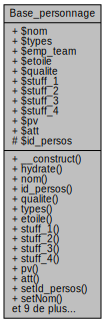
\includegraphics[width=177pt]{class_base__personnage__coll__graph}
\end{center}
\end{figure}
\subsection*{Fonctions membres publiques}
\begin{DoxyCompactItemize}
\item 
\mbox{\hyperlink{class_base__personnage_adc8ce28bfa1d2fffd9e568fbb25a0104}{\+\_\+\+\_\+construct}} (\$valeurs=array())
\item 
\mbox{\hyperlink{class_base__personnage_a100783dd2f191636d3eab860a60c18f6}{hydrate}} (array \$donnees)
\item 
\mbox{\hyperlink{class_base__personnage_abd3b2c38016dc7f95b967225d4dfbd17}{nom}} ()
\item 
\mbox{\hyperlink{class_base__personnage_ab840c279a1234075b5598b6bc48c0288}{id\+\_\+persos}} ()
\item 
\mbox{\hyperlink{class_base__personnage_a77daa43282aa9b4653c70b4a97dc7948}{qualite}} ()
\item 
\mbox{\hyperlink{class_base__personnage_a24e406f1e1d2c35596ccd5a6627c5650}{types}} ()
\item 
\mbox{\hyperlink{class_base__personnage_a17546eb34101fa1d501e84309f3f806c}{etoile}} ()
\item 
\mbox{\hyperlink{class_base__personnage_aad70521301b01ab3918bea05bef7b54b}{stuff\+\_\+1}} ()
\item 
\mbox{\hyperlink{class_base__personnage_ae37a88e0e1535ff5f0d786c1007fbe1e}{stuff\+\_\+2}} ()
\item 
\mbox{\hyperlink{class_base__personnage_a901d3c830ec965886fcf9c57ff153675}{stuff\+\_\+3}} ()
\item 
\mbox{\hyperlink{class_base__personnage_afb797796a81d9bec991ede838c711bd6}{stuff\+\_\+4}} ()
\item 
\mbox{\hyperlink{class_base__personnage_a2b94389a8a3b5538c0b01e36f3ca55bf}{pv}} ()
\item 
\mbox{\hyperlink{class_base__personnage_ad09642245bba8747d0ebd3ab991c66b9}{att}} ()
\item 
\mbox{\hyperlink{class_base__personnage_a14498c5c6a7ced9420401351eacf2ecf}{set\+Id\+\_\+persos}} (\$\mbox{\hyperlink{class_base__personnage_ab840c279a1234075b5598b6bc48c0288}{id\+\_\+persos}})
\item 
\mbox{\hyperlink{class_base__personnage_a44eae499b82470a6c99e01b68a73a6d9}{set\+Nom}} (\$\mbox{\hyperlink{class_base__personnage_abd3b2c38016dc7f95b967225d4dfbd17}{nom}})
\item 
\mbox{\hyperlink{class_base__personnage_a05dbaa079c1220db181bd98a204ffead}{set\+Qualite}} (\$\mbox{\hyperlink{class_base__personnage_a77daa43282aa9b4653c70b4a97dc7948}{qualite}})
\item 
\mbox{\hyperlink{class_base__personnage_aa3d0dbf11be8d919e4faa6e7f110375e}{set\+Types}} (\$\mbox{\hyperlink{class_base__personnage_a24e406f1e1d2c35596ccd5a6627c5650}{types}})
\item 
\mbox{\hyperlink{class_base__personnage_aa16912b89559e2aa9c96e2d1b2cd9d4f}{set\+Pv}} (\$\mbox{\hyperlink{class_base__personnage_a2b94389a8a3b5538c0b01e36f3ca55bf}{pv}})
\item 
\mbox{\hyperlink{class_base__personnage_a4c64fc057282c154957efe45c601f551}{set\+Att}} (\$\mbox{\hyperlink{class_base__personnage_ad09642245bba8747d0ebd3ab991c66b9}{att}})
\item 
\mbox{\hyperlink{class_base__personnage_a8aeece8f59864d993f5a571bac2d4dd6}{set\+Emp\+\_\+team}} (\$emp\+\_\+team)
\item 
\mbox{\hyperlink{class_base__personnage_a1044ae4053449cbf15bad1700e47f05d}{set\+Stuff\+\_\+1}} (\$\mbox{\hyperlink{class_base__personnage_aad70521301b01ab3918bea05bef7b54b}{stuff\+\_\+1}})
\item 
\mbox{\hyperlink{class_base__personnage_abebf595054cb225477f869946d9ac1ae}{set\+Stuff\+\_\+2}} (\$\mbox{\hyperlink{class_base__personnage_ae37a88e0e1535ff5f0d786c1007fbe1e}{stuff\+\_\+2}})
\item 
\mbox{\hyperlink{class_base__personnage_a7a57cd139690c7a92bf886773171fe86}{set\+Stuff\+\_\+3}} (\$\mbox{\hyperlink{class_base__personnage_a901d3c830ec965886fcf9c57ff153675}{stuff\+\_\+3}})
\item 
\mbox{\hyperlink{class_base__personnage_a19983536bab7533d81e56f5ca2934f2c}{set\+Stuff\+\_\+4}} (\$\mbox{\hyperlink{class_base__personnage_afb797796a81d9bec991ede838c711bd6}{stuff\+\_\+4}})
\end{DoxyCompactItemize}
\subsection*{Champs de données}
\begin{DoxyCompactItemize}
\item 
\mbox{\hyperlink{class_base__personnage_afd27c4f68e90081ac017ad811ceecc13}{\$nom}}
\item 
\mbox{\hyperlink{class_base__personnage_a9b93bd32a21d0fbecdd136edc1b5d4e4}{\$types}}
\item 
\mbox{\hyperlink{class_base__personnage_a2c671bc973d3bb997ecce969fc120b5f}{\$emp\+\_\+team}}
\item 
\mbox{\hyperlink{class_base__personnage_ae3abe8ba29b0b4af469fc48af7350f25}{\$etoile}}
\item 
\mbox{\hyperlink{class_base__personnage_a740e0ca5d6d55c3d196c465749504e0d}{\$qualite}}
\item 
\mbox{\hyperlink{class_base__personnage_a15cf5869509ee2bad46d637b1ec3e7d0}{\$stuff\+\_\+1}}
\item 
\mbox{\hyperlink{class_base__personnage_a4e35acccaa1e6ef3a08f3c31f6a2dc4c}{\$stuff\+\_\+2}}
\item 
\mbox{\hyperlink{class_base__personnage_a3c2204adf2a89f3bfff1cab97f460292}{\$stuff\+\_\+3}}
\item 
\mbox{\hyperlink{class_base__personnage_a388da9ed289cf32963323619f228554b}{\$stuff\+\_\+4}}
\item 
\mbox{\hyperlink{class_base__personnage_aa052dcb8719da97edec439217353a80b}{\$pv}}
\item 
\mbox{\hyperlink{class_base__personnage_a95a0c782140918824dcb403e4fe83db4}{\$att}}
\end{DoxyCompactItemize}
\subsection*{Attributs protégés}
\begin{DoxyCompactItemize}
\item 
\mbox{\hyperlink{class_base__personnage_a806b0b0a15951b2415539bd9560b7808}{\$id\+\_\+persos}}
\end{DoxyCompactItemize}


\subsection{Description détaillée}


Définition à la ligne 13 du fichier Base\+\_\+personnage.\+php.



\subsection{Documentation des constructeurs et destructeur}
\mbox{\Hypertarget{class_base__personnage_adc8ce28bfa1d2fffd9e568fbb25a0104}\label{class_base__personnage_adc8ce28bfa1d2fffd9e568fbb25a0104}} 
\index{Base\+\_\+personnage@{Base\+\_\+personnage}!\+\_\+\+\_\+construct@{\+\_\+\+\_\+construct}}
\index{\+\_\+\+\_\+construct@{\+\_\+\+\_\+construct}!Base\+\_\+personnage@{Base\+\_\+personnage}}
\subsubsection{\texorpdfstring{\+\_\+\+\_\+construct()}{\_\_construct()}}
{\footnotesize\ttfamily Base\+\_\+personnage\+::\+\_\+\+\_\+construct (\begin{DoxyParamCaption}\item[{}]{\$valeurs = {\ttfamily array()} }\end{DoxyParamCaption})}



Définition à la ligne 27 du fichier Base\+\_\+personnage.\+php.

Voici le graphe d\textquotesingle{}appel pour cette fonction \+:\nopagebreak
\begin{figure}[H]
\begin{center}
\leavevmode
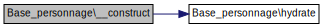
\includegraphics[width=350pt]{class_base__personnage_adc8ce28bfa1d2fffd9e568fbb25a0104_cgraph}
\end{center}
\end{figure}


\subsection{Documentation des fonctions membres}
\mbox{\Hypertarget{class_base__personnage_ad09642245bba8747d0ebd3ab991c66b9}\label{class_base__personnage_ad09642245bba8747d0ebd3ab991c66b9}} 
\index{Base\+\_\+personnage@{Base\+\_\+personnage}!att@{att}}
\index{att@{att}!Base\+\_\+personnage@{Base\+\_\+personnage}}
\subsubsection{\texorpdfstring{att()}{att()}}
{\footnotesize\ttfamily Base\+\_\+personnage\+::att (\begin{DoxyParamCaption}{ }\end{DoxyParamCaption})}



Définition à la ligne 63 du fichier Base\+\_\+personnage.\+php.

Voici le graphe des appelants de cette fonction \+:\nopagebreak
\begin{figure}[H]
\begin{center}
\leavevmode
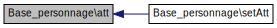
\includegraphics[width=350pt]{class_base__personnage_ad09642245bba8747d0ebd3ab991c66b9_icgraph}
\end{center}
\end{figure}
\mbox{\Hypertarget{class_base__personnage_a17546eb34101fa1d501e84309f3f806c}\label{class_base__personnage_a17546eb34101fa1d501e84309f3f806c}} 
\index{Base\+\_\+personnage@{Base\+\_\+personnage}!etoile@{etoile}}
\index{etoile@{etoile}!Base\+\_\+personnage@{Base\+\_\+personnage}}
\subsubsection{\texorpdfstring{etoile()}{etoile()}}
{\footnotesize\ttfamily Base\+\_\+personnage\+::etoile (\begin{DoxyParamCaption}{ }\end{DoxyParamCaption})}



Définition à la ligne 57 du fichier Base\+\_\+personnage.\+php.

\mbox{\Hypertarget{class_base__personnage_a100783dd2f191636d3eab860a60c18f6}\label{class_base__personnage_a100783dd2f191636d3eab860a60c18f6}} 
\index{Base\+\_\+personnage@{Base\+\_\+personnage}!hydrate@{hydrate}}
\index{hydrate@{hydrate}!Base\+\_\+personnage@{Base\+\_\+personnage}}
\subsubsection{\texorpdfstring{hydrate()}{hydrate()}}
{\footnotesize\ttfamily Base\+\_\+personnage\+::hydrate (\begin{DoxyParamCaption}\item[{array}]{\$donnees }\end{DoxyParamCaption})}



Définition à la ligne 35 du fichier Base\+\_\+personnage.\+php.

Voici le graphe des appelants de cette fonction \+:\nopagebreak
\begin{figure}[H]
\begin{center}
\leavevmode
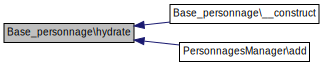
\includegraphics[width=350pt]{class_base__personnage_a100783dd2f191636d3eab860a60c18f6_icgraph}
\end{center}
\end{figure}
\mbox{\Hypertarget{class_base__personnage_ab840c279a1234075b5598b6bc48c0288}\label{class_base__personnage_ab840c279a1234075b5598b6bc48c0288}} 
\index{Base\+\_\+personnage@{Base\+\_\+personnage}!id\+\_\+persos@{id\+\_\+persos}}
\index{id\+\_\+persos@{id\+\_\+persos}!Base\+\_\+personnage@{Base\+\_\+personnage}}
\subsubsection{\texorpdfstring{id\+\_\+persos()}{id\_persos()}}
{\footnotesize\ttfamily Base\+\_\+personnage\+::id\+\_\+persos (\begin{DoxyParamCaption}{ }\end{DoxyParamCaption})}



Définition à la ligne 54 du fichier Base\+\_\+personnage.\+php.

Voici le graphe des appelants de cette fonction \+:\nopagebreak
\begin{figure}[H]
\begin{center}
\leavevmode
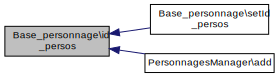
\includegraphics[width=345pt]{class_base__personnage_ab840c279a1234075b5598b6bc48c0288_icgraph}
\end{center}
\end{figure}
\mbox{\Hypertarget{class_base__personnage_abd3b2c38016dc7f95b967225d4dfbd17}\label{class_base__personnage_abd3b2c38016dc7f95b967225d4dfbd17}} 
\index{Base\+\_\+personnage@{Base\+\_\+personnage}!nom@{nom}}
\index{nom@{nom}!Base\+\_\+personnage@{Base\+\_\+personnage}}
\subsubsection{\texorpdfstring{nom()}{nom()}}
{\footnotesize\ttfamily Base\+\_\+personnage\+::nom (\begin{DoxyParamCaption}{ }\end{DoxyParamCaption})}



Définition à la ligne 53 du fichier Base\+\_\+personnage.\+php.

Voici le graphe des appelants de cette fonction \+:\nopagebreak
\begin{figure}[H]
\begin{center}
\leavevmode
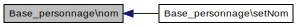
\includegraphics[width=350pt]{class_base__personnage_abd3b2c38016dc7f95b967225d4dfbd17_icgraph}
\end{center}
\end{figure}
\mbox{\Hypertarget{class_base__personnage_a2b94389a8a3b5538c0b01e36f3ca55bf}\label{class_base__personnage_a2b94389a8a3b5538c0b01e36f3ca55bf}} 
\index{Base\+\_\+personnage@{Base\+\_\+personnage}!pv@{pv}}
\index{pv@{pv}!Base\+\_\+personnage@{Base\+\_\+personnage}}
\subsubsection{\texorpdfstring{pv()}{pv()}}
{\footnotesize\ttfamily Base\+\_\+personnage\+::pv (\begin{DoxyParamCaption}{ }\end{DoxyParamCaption})}



Définition à la ligne 62 du fichier Base\+\_\+personnage.\+php.

Voici le graphe des appelants de cette fonction \+:\nopagebreak
\begin{figure}[H]
\begin{center}
\leavevmode
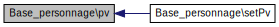
\includegraphics[width=350pt]{class_base__personnage_a2b94389a8a3b5538c0b01e36f3ca55bf_icgraph}
\end{center}
\end{figure}
\mbox{\Hypertarget{class_base__personnage_a77daa43282aa9b4653c70b4a97dc7948}\label{class_base__personnage_a77daa43282aa9b4653c70b4a97dc7948}} 
\index{Base\+\_\+personnage@{Base\+\_\+personnage}!qualite@{qualite}}
\index{qualite@{qualite}!Base\+\_\+personnage@{Base\+\_\+personnage}}
\subsubsection{\texorpdfstring{qualite()}{qualite()}}
{\footnotesize\ttfamily Base\+\_\+personnage\+::qualite (\begin{DoxyParamCaption}{ }\end{DoxyParamCaption})}



Définition à la ligne 55 du fichier Base\+\_\+personnage.\+php.

Voici le graphe des appelants de cette fonction \+:\nopagebreak
\begin{figure}[H]
\begin{center}
\leavevmode
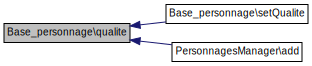
\includegraphics[width=350pt]{class_base__personnage_a77daa43282aa9b4653c70b4a97dc7948_icgraph}
\end{center}
\end{figure}
\mbox{\Hypertarget{class_base__personnage_a4c64fc057282c154957efe45c601f551}\label{class_base__personnage_a4c64fc057282c154957efe45c601f551}} 
\index{Base\+\_\+personnage@{Base\+\_\+personnage}!set\+Att@{set\+Att}}
\index{set\+Att@{set\+Att}!Base\+\_\+personnage@{Base\+\_\+personnage}}
\subsubsection{\texorpdfstring{set\+Att()}{setAtt()}}
{\footnotesize\ttfamily Base\+\_\+personnage\+::set\+Att (\begin{DoxyParamCaption}\item[{}]{\$att }\end{DoxyParamCaption})}



Définition à la ligne 114 du fichier Base\+\_\+personnage.\+php.

Voici le graphe d\textquotesingle{}appel pour cette fonction \+:\nopagebreak
\begin{figure}[H]
\begin{center}
\leavevmode
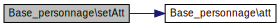
\includegraphics[width=350pt]{class_base__personnage_a4c64fc057282c154957efe45c601f551_cgraph}
\end{center}
\end{figure}
\mbox{\Hypertarget{class_base__personnage_a8aeece8f59864d993f5a571bac2d4dd6}\label{class_base__personnage_a8aeece8f59864d993f5a571bac2d4dd6}} 
\index{Base\+\_\+personnage@{Base\+\_\+personnage}!set\+Emp\+\_\+team@{set\+Emp\+\_\+team}}
\index{set\+Emp\+\_\+team@{set\+Emp\+\_\+team}!Base\+\_\+personnage@{Base\+\_\+personnage}}
\subsubsection{\texorpdfstring{set\+Emp\+\_\+team()}{setEmp\_team()}}
{\footnotesize\ttfamily Base\+\_\+personnage\+::set\+Emp\+\_\+team (\begin{DoxyParamCaption}\item[{}]{\$emp\+\_\+team }\end{DoxyParamCaption})}



Définition à la ligne 125 du fichier Base\+\_\+personnage.\+php.

\mbox{\Hypertarget{class_base__personnage_a14498c5c6a7ced9420401351eacf2ecf}\label{class_base__personnage_a14498c5c6a7ced9420401351eacf2ecf}} 
\index{Base\+\_\+personnage@{Base\+\_\+personnage}!set\+Id\+\_\+persos@{set\+Id\+\_\+persos}}
\index{set\+Id\+\_\+persos@{set\+Id\+\_\+persos}!Base\+\_\+personnage@{Base\+\_\+personnage}}
\subsubsection{\texorpdfstring{set\+Id\+\_\+persos()}{setId\_persos()}}
{\footnotesize\ttfamily Base\+\_\+personnage\+::set\+Id\+\_\+persos (\begin{DoxyParamCaption}\item[{}]{\$id\+\_\+persos }\end{DoxyParamCaption})}



Définition à la ligne 67 du fichier Base\+\_\+personnage.\+php.

Voici le graphe d\textquotesingle{}appel pour cette fonction \+:\nopagebreak
\begin{figure}[H]
\begin{center}
\leavevmode
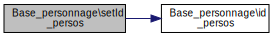
\includegraphics[width=345pt]{class_base__personnage_a14498c5c6a7ced9420401351eacf2ecf_cgraph}
\end{center}
\end{figure}
\mbox{\Hypertarget{class_base__personnage_a44eae499b82470a6c99e01b68a73a6d9}\label{class_base__personnage_a44eae499b82470a6c99e01b68a73a6d9}} 
\index{Base\+\_\+personnage@{Base\+\_\+personnage}!set\+Nom@{set\+Nom}}
\index{set\+Nom@{set\+Nom}!Base\+\_\+personnage@{Base\+\_\+personnage}}
\subsubsection{\texorpdfstring{set\+Nom()}{setNom()}}
{\footnotesize\ttfamily Base\+\_\+personnage\+::set\+Nom (\begin{DoxyParamCaption}\item[{}]{\$nom }\end{DoxyParamCaption})}



Définition à la ligne 73 du fichier Base\+\_\+personnage.\+php.

Voici le graphe d\textquotesingle{}appel pour cette fonction \+:\nopagebreak
\begin{figure}[H]
\begin{center}
\leavevmode
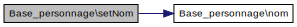
\includegraphics[width=350pt]{class_base__personnage_a44eae499b82470a6c99e01b68a73a6d9_cgraph}
\end{center}
\end{figure}
\mbox{\Hypertarget{class_base__personnage_aa16912b89559e2aa9c96e2d1b2cd9d4f}\label{class_base__personnage_aa16912b89559e2aa9c96e2d1b2cd9d4f}} 
\index{Base\+\_\+personnage@{Base\+\_\+personnage}!set\+Pv@{set\+Pv}}
\index{set\+Pv@{set\+Pv}!Base\+\_\+personnage@{Base\+\_\+personnage}}
\subsubsection{\texorpdfstring{set\+Pv()}{setPv()}}
{\footnotesize\ttfamily Base\+\_\+personnage\+::set\+Pv (\begin{DoxyParamCaption}\item[{}]{\$pv }\end{DoxyParamCaption})}



Définition à la ligne 103 du fichier Base\+\_\+personnage.\+php.

Voici le graphe d\textquotesingle{}appel pour cette fonction \+:\nopagebreak
\begin{figure}[H]
\begin{center}
\leavevmode
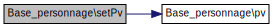
\includegraphics[width=350pt]{class_base__personnage_aa16912b89559e2aa9c96e2d1b2cd9d4f_cgraph}
\end{center}
\end{figure}
\mbox{\Hypertarget{class_base__personnage_a05dbaa079c1220db181bd98a204ffead}\label{class_base__personnage_a05dbaa079c1220db181bd98a204ffead}} 
\index{Base\+\_\+personnage@{Base\+\_\+personnage}!set\+Qualite@{set\+Qualite}}
\index{set\+Qualite@{set\+Qualite}!Base\+\_\+personnage@{Base\+\_\+personnage}}
\subsubsection{\texorpdfstring{set\+Qualite()}{setQualite()}}
{\footnotesize\ttfamily Base\+\_\+personnage\+::set\+Qualite (\begin{DoxyParamCaption}\item[{}]{\$qualite }\end{DoxyParamCaption})}



Définition à la ligne 83 du fichier Base\+\_\+personnage.\+php.

Voici le graphe d\textquotesingle{}appel pour cette fonction \+:\nopagebreak
\begin{figure}[H]
\begin{center}
\leavevmode
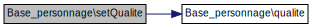
\includegraphics[width=350pt]{class_base__personnage_a05dbaa079c1220db181bd98a204ffead_cgraph}
\end{center}
\end{figure}
\mbox{\Hypertarget{class_base__personnage_a1044ae4053449cbf15bad1700e47f05d}\label{class_base__personnage_a1044ae4053449cbf15bad1700e47f05d}} 
\index{Base\+\_\+personnage@{Base\+\_\+personnage}!set\+Stuff\+\_\+1@{set\+Stuff\+\_\+1}}
\index{set\+Stuff\+\_\+1@{set\+Stuff\+\_\+1}!Base\+\_\+personnage@{Base\+\_\+personnage}}
\subsubsection{\texorpdfstring{set\+Stuff\+\_\+1()}{setStuff\_1()}}
{\footnotesize\ttfamily Base\+\_\+personnage\+::set\+Stuff\+\_\+1 (\begin{DoxyParamCaption}\item[{}]{\$stuff\+\_\+1 }\end{DoxyParamCaption})}



Définition à la ligne 136 du fichier Base\+\_\+personnage.\+php.

Voici le graphe d\textquotesingle{}appel pour cette fonction \+:\nopagebreak
\begin{figure}[H]
\begin{center}
\leavevmode
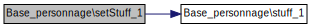
\includegraphics[width=350pt]{class_base__personnage_a1044ae4053449cbf15bad1700e47f05d_cgraph}
\end{center}
\end{figure}
\mbox{\Hypertarget{class_base__personnage_abebf595054cb225477f869946d9ac1ae}\label{class_base__personnage_abebf595054cb225477f869946d9ac1ae}} 
\index{Base\+\_\+personnage@{Base\+\_\+personnage}!set\+Stuff\+\_\+2@{set\+Stuff\+\_\+2}}
\index{set\+Stuff\+\_\+2@{set\+Stuff\+\_\+2}!Base\+\_\+personnage@{Base\+\_\+personnage}}
\subsubsection{\texorpdfstring{set\+Stuff\+\_\+2()}{setStuff\_2()}}
{\footnotesize\ttfamily Base\+\_\+personnage\+::set\+Stuff\+\_\+2 (\begin{DoxyParamCaption}\item[{}]{\$stuff\+\_\+2 }\end{DoxyParamCaption})}



Définition à la ligne 147 du fichier Base\+\_\+personnage.\+php.

Voici le graphe d\textquotesingle{}appel pour cette fonction \+:\nopagebreak
\begin{figure}[H]
\begin{center}
\leavevmode
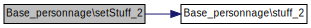
\includegraphics[width=350pt]{class_base__personnage_abebf595054cb225477f869946d9ac1ae_cgraph}
\end{center}
\end{figure}
\mbox{\Hypertarget{class_base__personnage_a7a57cd139690c7a92bf886773171fe86}\label{class_base__personnage_a7a57cd139690c7a92bf886773171fe86}} 
\index{Base\+\_\+personnage@{Base\+\_\+personnage}!set\+Stuff\+\_\+3@{set\+Stuff\+\_\+3}}
\index{set\+Stuff\+\_\+3@{set\+Stuff\+\_\+3}!Base\+\_\+personnage@{Base\+\_\+personnage}}
\subsubsection{\texorpdfstring{set\+Stuff\+\_\+3()}{setStuff\_3()}}
{\footnotesize\ttfamily Base\+\_\+personnage\+::set\+Stuff\+\_\+3 (\begin{DoxyParamCaption}\item[{}]{\$stuff\+\_\+3 }\end{DoxyParamCaption})}



Définition à la ligne 158 du fichier Base\+\_\+personnage.\+php.

Voici le graphe d\textquotesingle{}appel pour cette fonction \+:\nopagebreak
\begin{figure}[H]
\begin{center}
\leavevmode
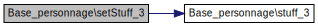
\includegraphics[width=350pt]{class_base__personnage_a7a57cd139690c7a92bf886773171fe86_cgraph}
\end{center}
\end{figure}
\mbox{\Hypertarget{class_base__personnage_a19983536bab7533d81e56f5ca2934f2c}\label{class_base__personnage_a19983536bab7533d81e56f5ca2934f2c}} 
\index{Base\+\_\+personnage@{Base\+\_\+personnage}!set\+Stuff\+\_\+4@{set\+Stuff\+\_\+4}}
\index{set\+Stuff\+\_\+4@{set\+Stuff\+\_\+4}!Base\+\_\+personnage@{Base\+\_\+personnage}}
\subsubsection{\texorpdfstring{set\+Stuff\+\_\+4()}{setStuff\_4()}}
{\footnotesize\ttfamily Base\+\_\+personnage\+::set\+Stuff\+\_\+4 (\begin{DoxyParamCaption}\item[{}]{\$stuff\+\_\+4 }\end{DoxyParamCaption})}



Définition à la ligne 169 du fichier Base\+\_\+personnage.\+php.

Voici le graphe d\textquotesingle{}appel pour cette fonction \+:\nopagebreak
\begin{figure}[H]
\begin{center}
\leavevmode
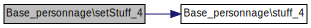
\includegraphics[width=350pt]{class_base__personnage_a19983536bab7533d81e56f5ca2934f2c_cgraph}
\end{center}
\end{figure}
\mbox{\Hypertarget{class_base__personnage_aa3d0dbf11be8d919e4faa6e7f110375e}\label{class_base__personnage_aa3d0dbf11be8d919e4faa6e7f110375e}} 
\index{Base\+\_\+personnage@{Base\+\_\+personnage}!set\+Types@{set\+Types}}
\index{set\+Types@{set\+Types}!Base\+\_\+personnage@{Base\+\_\+personnage}}
\subsubsection{\texorpdfstring{set\+Types()}{setTypes()}}
{\footnotesize\ttfamily Base\+\_\+personnage\+::set\+Types (\begin{DoxyParamCaption}\item[{}]{\$types }\end{DoxyParamCaption})}



Définition à la ligne 93 du fichier Base\+\_\+personnage.\+php.

Voici le graphe d\textquotesingle{}appel pour cette fonction \+:\nopagebreak
\begin{figure}[H]
\begin{center}
\leavevmode
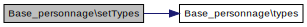
\includegraphics[width=350pt]{class_base__personnage_aa3d0dbf11be8d919e4faa6e7f110375e_cgraph}
\end{center}
\end{figure}
\mbox{\Hypertarget{class_base__personnage_aad70521301b01ab3918bea05bef7b54b}\label{class_base__personnage_aad70521301b01ab3918bea05bef7b54b}} 
\index{Base\+\_\+personnage@{Base\+\_\+personnage}!stuff\+\_\+1@{stuff\+\_\+1}}
\index{stuff\+\_\+1@{stuff\+\_\+1}!Base\+\_\+personnage@{Base\+\_\+personnage}}
\subsubsection{\texorpdfstring{stuff\+\_\+1()}{stuff\_1()}}
{\footnotesize\ttfamily Base\+\_\+personnage\+::stuff\+\_\+1 (\begin{DoxyParamCaption}{ }\end{DoxyParamCaption})}



Définition à la ligne 58 du fichier Base\+\_\+personnage.\+php.

Voici le graphe des appelants de cette fonction \+:\nopagebreak
\begin{figure}[H]
\begin{center}
\leavevmode
\includegraphics[width=350pt]{class_base__personnage_aad70521301b01ab3918bea05bef7b54b_icgraph}
\end{center}
\end{figure}
\mbox{\Hypertarget{class_base__personnage_ae37a88e0e1535ff5f0d786c1007fbe1e}\label{class_base__personnage_ae37a88e0e1535ff5f0d786c1007fbe1e}} 
\index{Base\+\_\+personnage@{Base\+\_\+personnage}!stuff\+\_\+2@{stuff\+\_\+2}}
\index{stuff\+\_\+2@{stuff\+\_\+2}!Base\+\_\+personnage@{Base\+\_\+personnage}}
\subsubsection{\texorpdfstring{stuff\+\_\+2()}{stuff\_2()}}
{\footnotesize\ttfamily Base\+\_\+personnage\+::stuff\+\_\+2 (\begin{DoxyParamCaption}{ }\end{DoxyParamCaption})}



Définition à la ligne 59 du fichier Base\+\_\+personnage.\+php.

Voici le graphe des appelants de cette fonction \+:\nopagebreak
\begin{figure}[H]
\begin{center}
\leavevmode
\includegraphics[width=350pt]{class_base__personnage_ae37a88e0e1535ff5f0d786c1007fbe1e_icgraph}
\end{center}
\end{figure}
\mbox{\Hypertarget{class_base__personnage_a901d3c830ec965886fcf9c57ff153675}\label{class_base__personnage_a901d3c830ec965886fcf9c57ff153675}} 
\index{Base\+\_\+personnage@{Base\+\_\+personnage}!stuff\+\_\+3@{stuff\+\_\+3}}
\index{stuff\+\_\+3@{stuff\+\_\+3}!Base\+\_\+personnage@{Base\+\_\+personnage}}
\subsubsection{\texorpdfstring{stuff\+\_\+3()}{stuff\_3()}}
{\footnotesize\ttfamily Base\+\_\+personnage\+::stuff\+\_\+3 (\begin{DoxyParamCaption}{ }\end{DoxyParamCaption})}



Définition à la ligne 60 du fichier Base\+\_\+personnage.\+php.

Voici le graphe des appelants de cette fonction \+:\nopagebreak
\begin{figure}[H]
\begin{center}
\leavevmode
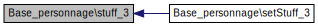
\includegraphics[width=350pt]{class_base__personnage_a901d3c830ec965886fcf9c57ff153675_icgraph}
\end{center}
\end{figure}
\mbox{\Hypertarget{class_base__personnage_afb797796a81d9bec991ede838c711bd6}\label{class_base__personnage_afb797796a81d9bec991ede838c711bd6}} 
\index{Base\+\_\+personnage@{Base\+\_\+personnage}!stuff\+\_\+4@{stuff\+\_\+4}}
\index{stuff\+\_\+4@{stuff\+\_\+4}!Base\+\_\+personnage@{Base\+\_\+personnage}}
\subsubsection{\texorpdfstring{stuff\+\_\+4()}{stuff\_4()}}
{\footnotesize\ttfamily Base\+\_\+personnage\+::stuff\+\_\+4 (\begin{DoxyParamCaption}{ }\end{DoxyParamCaption})}



Définition à la ligne 61 du fichier Base\+\_\+personnage.\+php.

Voici le graphe des appelants de cette fonction \+:\nopagebreak
\begin{figure}[H]
\begin{center}
\leavevmode
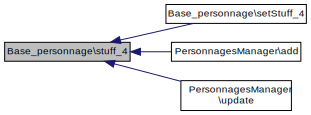
\includegraphics[width=350pt]{class_base__personnage_afb797796a81d9bec991ede838c711bd6_icgraph}
\end{center}
\end{figure}
\mbox{\Hypertarget{class_base__personnage_a24e406f1e1d2c35596ccd5a6627c5650}\label{class_base__personnage_a24e406f1e1d2c35596ccd5a6627c5650}} 
\index{Base\+\_\+personnage@{Base\+\_\+personnage}!types@{types}}
\index{types@{types}!Base\+\_\+personnage@{Base\+\_\+personnage}}
\subsubsection{\texorpdfstring{types()}{types()}}
{\footnotesize\ttfamily Base\+\_\+personnage\+::types (\begin{DoxyParamCaption}{ }\end{DoxyParamCaption})}



Définition à la ligne 56 du fichier Base\+\_\+personnage.\+php.

Voici le graphe des appelants de cette fonction \+:\nopagebreak
\begin{figure}[H]
\begin{center}
\leavevmode
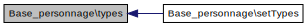
\includegraphics[width=350pt]{class_base__personnage_a24e406f1e1d2c35596ccd5a6627c5650_icgraph}
\end{center}
\end{figure}


\subsection{Documentation des champs}
\mbox{\Hypertarget{class_base__personnage_a95a0c782140918824dcb403e4fe83db4}\label{class_base__personnage_a95a0c782140918824dcb403e4fe83db4}} 
\index{Base\+\_\+personnage@{Base\+\_\+personnage}!\$att@{\$att}}
\index{\$att@{\$att}!Base\+\_\+personnage@{Base\+\_\+personnage}}
\subsubsection{\texorpdfstring{\$att}{$att}}
{\footnotesize\ttfamily Base\+\_\+personnage\+::\$att}

degat du personnage 

Définition à la ligne 14 du fichier Base\+\_\+personnage.\+php.

\mbox{\Hypertarget{class_base__personnage_a2c671bc973d3bb997ecce969fc120b5f}\label{class_base__personnage_a2c671bc973d3bb997ecce969fc120b5f}} 
\index{Base\+\_\+personnage@{Base\+\_\+personnage}!\$emp\+\_\+team@{\$emp\+\_\+team}}
\index{\$emp\+\_\+team@{\$emp\+\_\+team}!Base\+\_\+personnage@{Base\+\_\+personnage}}
\subsubsection{\texorpdfstring{\$emp\+\_\+team}{$emp\_team}}
{\footnotesize\ttfamily Base\+\_\+personnage\+::\$emp\+\_\+team}

emplacement si dans l\textquotesingle{}équipe 

Définition à la ligne 14 du fichier Base\+\_\+personnage.\+php.

\mbox{\Hypertarget{class_base__personnage_ae3abe8ba29b0b4af469fc48af7350f25}\label{class_base__personnage_ae3abe8ba29b0b4af469fc48af7350f25}} 
\index{Base\+\_\+personnage@{Base\+\_\+personnage}!\$etoile@{\$etoile}}
\index{\$etoile@{\$etoile}!Base\+\_\+personnage@{Base\+\_\+personnage}}
\subsubsection{\texorpdfstring{\$etoile}{$etoile}}
{\footnotesize\ttfamily Base\+\_\+personnage\+::\$etoile}

étoile du personnage 

Définition à la ligne 14 du fichier Base\+\_\+personnage.\+php.

\mbox{\Hypertarget{class_base__personnage_a806b0b0a15951b2415539bd9560b7808}\label{class_base__personnage_a806b0b0a15951b2415539bd9560b7808}} 
\index{Base\+\_\+personnage@{Base\+\_\+personnage}!\$id\+\_\+persos@{\$id\+\_\+persos}}
\index{\$id\+\_\+persos@{\$id\+\_\+persos}!Base\+\_\+personnage@{Base\+\_\+personnage}}
\subsubsection{\texorpdfstring{\$id\+\_\+persos}{$id\_persos}}
{\footnotesize\ttfamily Base\+\_\+personnage\+::\$id\+\_\+persos\hspace{0.3cm}{\ttfamily [protected]}}

id du personnage 

Définition à la ligne 14 du fichier Base\+\_\+personnage.\+php.

\mbox{\Hypertarget{class_base__personnage_afd27c4f68e90081ac017ad811ceecc13}\label{class_base__personnage_afd27c4f68e90081ac017ad811ceecc13}} 
\index{Base\+\_\+personnage@{Base\+\_\+personnage}!\$nom@{\$nom}}
\index{\$nom@{\$nom}!Base\+\_\+personnage@{Base\+\_\+personnage}}
\subsubsection{\texorpdfstring{\$nom}{$nom}}
{\footnotesize\ttfamily Base\+\_\+personnage\+::\$nom}

nom du personnage 

Définition à la ligne 14 du fichier Base\+\_\+personnage.\+php.

\mbox{\Hypertarget{class_base__personnage_aa052dcb8719da97edec439217353a80b}\label{class_base__personnage_aa052dcb8719da97edec439217353a80b}} 
\index{Base\+\_\+personnage@{Base\+\_\+personnage}!\$pv@{\$pv}}
\index{\$pv@{\$pv}!Base\+\_\+personnage@{Base\+\_\+personnage}}
\subsubsection{\texorpdfstring{\$pv}{$pv}}
{\footnotesize\ttfamily Base\+\_\+personnage\+::\$pv}

point de vie du personnage 

Définition à la ligne 14 du fichier Base\+\_\+personnage.\+php.

\mbox{\Hypertarget{class_base__personnage_a740e0ca5d6d55c3d196c465749504e0d}\label{class_base__personnage_a740e0ca5d6d55c3d196c465749504e0d}} 
\index{Base\+\_\+personnage@{Base\+\_\+personnage}!\$qualite@{\$qualite}}
\index{\$qualite@{\$qualite}!Base\+\_\+personnage@{Base\+\_\+personnage}}
\subsubsection{\texorpdfstring{\$qualite}{$qualite}}
{\footnotesize\ttfamily Base\+\_\+personnage\+::\$qualite}

qualité du personnage 

Définition à la ligne 14 du fichier Base\+\_\+personnage.\+php.

\mbox{\Hypertarget{class_base__personnage_a15cf5869509ee2bad46d637b1ec3e7d0}\label{class_base__personnage_a15cf5869509ee2bad46d637b1ec3e7d0}} 
\index{Base\+\_\+personnage@{Base\+\_\+personnage}!\$stuff\+\_\+1@{\$stuff\+\_\+1}}
\index{\$stuff\+\_\+1@{\$stuff\+\_\+1}!Base\+\_\+personnage@{Base\+\_\+personnage}}
\subsubsection{\texorpdfstring{\$stuff\+\_\+1}{$stuff\_1}}
{\footnotesize\ttfamily Base\+\_\+personnage\+::\$stuff\+\_\+1}

id de l\textquotesingle{}équipement n°1 

Définition à la ligne 14 du fichier Base\+\_\+personnage.\+php.

\mbox{\Hypertarget{class_base__personnage_a4e35acccaa1e6ef3a08f3c31f6a2dc4c}\label{class_base__personnage_a4e35acccaa1e6ef3a08f3c31f6a2dc4c}} 
\index{Base\+\_\+personnage@{Base\+\_\+personnage}!\$stuff\+\_\+2@{\$stuff\+\_\+2}}
\index{\$stuff\+\_\+2@{\$stuff\+\_\+2}!Base\+\_\+personnage@{Base\+\_\+personnage}}
\subsubsection{\texorpdfstring{\$stuff\+\_\+2}{$stuff\_2}}
{\footnotesize\ttfamily Base\+\_\+personnage\+::\$stuff\+\_\+2}

id de l\textquotesingle{}équipement n°2 

Définition à la ligne 14 du fichier Base\+\_\+personnage.\+php.

\mbox{\Hypertarget{class_base__personnage_a3c2204adf2a89f3bfff1cab97f460292}\label{class_base__personnage_a3c2204adf2a89f3bfff1cab97f460292}} 
\index{Base\+\_\+personnage@{Base\+\_\+personnage}!\$stuff\+\_\+3@{\$stuff\+\_\+3}}
\index{\$stuff\+\_\+3@{\$stuff\+\_\+3}!Base\+\_\+personnage@{Base\+\_\+personnage}}
\subsubsection{\texorpdfstring{\$stuff\+\_\+3}{$stuff\_3}}
{\footnotesize\ttfamily Base\+\_\+personnage\+::\$stuff\+\_\+3}

id de l\textquotesingle{}équipement n°3 

Définition à la ligne 14 du fichier Base\+\_\+personnage.\+php.

\mbox{\Hypertarget{class_base__personnage_a388da9ed289cf32963323619f228554b}\label{class_base__personnage_a388da9ed289cf32963323619f228554b}} 
\index{Base\+\_\+personnage@{Base\+\_\+personnage}!\$stuff\+\_\+4@{\$stuff\+\_\+4}}
\index{\$stuff\+\_\+4@{\$stuff\+\_\+4}!Base\+\_\+personnage@{Base\+\_\+personnage}}
\subsubsection{\texorpdfstring{\$stuff\+\_\+4}{$stuff\_4}}
{\footnotesize\ttfamily Base\+\_\+personnage\+::\$stuff\+\_\+4}

id de l\textquotesingle{}équipement n°4 , vide par default 

Définition à la ligne 14 du fichier Base\+\_\+personnage.\+php.

\mbox{\Hypertarget{class_base__personnage_a9b93bd32a21d0fbecdd136edc1b5d4e4}\label{class_base__personnage_a9b93bd32a21d0fbecdd136edc1b5d4e4}} 
\index{Base\+\_\+personnage@{Base\+\_\+personnage}!\$types@{\$types}}
\index{\$types@{\$types}!Base\+\_\+personnage@{Base\+\_\+personnage}}
\subsubsection{\texorpdfstring{\$types}{$types}}
{\footnotesize\ttfamily Base\+\_\+personnage\+::\$types}

type du personnage 

Définition à la ligne 14 du fichier Base\+\_\+personnage.\+php.



La documentation de cette classe a été générée à partir du fichier suivant \+:\begin{DoxyCompactItemize}
\item 
class/\mbox{\hyperlink{_base__personnage_8php}{Base\+\_\+personnage.\+php}}\end{DoxyCompactItemize}

\hypertarget{class_personnage}{}\section{Référence de la classe Personnage}
\label{class_personnage}\index{Personnage@{Personnage}}


{\ttfamily \#include \char`\"{}class/\+Personnage.\+php\char`\"{}}



Graphe d\textquotesingle{}héritage de Personnage\+:\nopagebreak
\begin{figure}[H]
\begin{center}
\leavevmode
\includegraphics[width=280pt]{class_personnage__inherit__graph}
\end{center}
\end{figure}


Graphe de collaboration de Personnage\+:\nopagebreak
\begin{figure}[H]
\begin{center}
\leavevmode
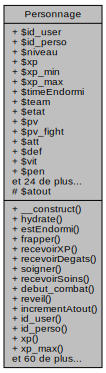
\includegraphics[width=179pt]{class_personnage__coll__graph}
\end{center}
\end{figure}
\subsection*{Fonctions membres publiques}
\begin{DoxyCompactItemize}
\item 
\mbox{\hyperlink{class_personnage_ad91c080e67c8a8487933af4a38ea46cb}{\+\_\+\+\_\+construct}} (\$valeurs=array())
\item 
\mbox{\hyperlink{class_personnage_ae95e51cac2f518a6a38d025f5580be3f}{hydrate}} (array \$donnees)
\item 
\mbox{\hyperlink{class_personnage_aabf0bcd80fcea089de16f33c029aae12}{est\+Endormi}} ()
\item 
\mbox{\hyperlink{class_personnage_a1deaeddff5bc8766d52da4fc2d0b8032}{frapper}} (\mbox{\hyperlink{class_personnage}{Personnage}} \$perso, \mbox{\hyperlink{class_personnage}{Personnage}} \$perso2)
\begin{DoxyCompactList}\small\item\em Fonction pour frapper. \end{DoxyCompactList}\item 
\mbox{\hyperlink{class_personnage_aa64edf7d4c080193213b12643eb05a5d}{recevoir\+XP}} (\$val)
\item 
\mbox{\hyperlink{class_personnage_a226affce78dca0151e0901896e58f14d}{recevoir\+Degats}} (\$perso2)
\item 
\mbox{\hyperlink{class_personnage_a1219171b9ddba0fecfa49995d7d71372}{soigner}} (\mbox{\hyperlink{class_personnage}{Personnage}} \$perso)
\item 
\mbox{\hyperlink{class_personnage_acadb61228a3ebdf18318771f954e2ae0}{recevoir\+Soins}} (\$perso)
\item 
\mbox{\hyperlink{class_personnage_a570935e88aa03fb191a3f06a41f5aec5}{debut\+\_\+combat}} ()
\item 
\mbox{\hyperlink{class_personnage_ab0503fe49e1a5403fe6d43d7d424e3ef}{reveil}} ()
\item 
\mbox{\hyperlink{class_personnage_a744674b144008a43e37036344accb378}{increment\+Atout}} ()
\item 
\mbox{\hyperlink{class_personnage_a83ccdd40630a166b7a1f5c84dd742e8c}{id\+\_\+user}} ()
\item 
\mbox{\hyperlink{class_personnage_aa34eed6a48eb3734596505b58497f2f1}{id\+\_\+perso}} ()
\item 
\mbox{\hyperlink{class_personnage_a60b2a6a44bc71517c063d87c062e0b87}{xp}} ()
\item 
\mbox{\hyperlink{class_personnage_aa5bc9f2bda281400fedbc1af1c19357d}{xp\+\_\+max}} ()
\item 
\mbox{\hyperlink{class_personnage_a061130b0c1c551d893ecffff2553cb93}{niveau}} ()
\item 
\mbox{\hyperlink{class_personnage_ae8daf1e07c298cf03a98b6b06d3adfd9}{qualite}} ()
\item 
\mbox{\hyperlink{class_personnage_ade67f55b78368cd7e3c92128bb7ae67d}{etoile}} ()
\item 
\mbox{\hyperlink{class_personnage_a54f0e416a628b1b7246f3c3a7c2081fa}{atout}} ()
\item 
\mbox{\hyperlink{class_personnage_a5fbe8f1f41e05e856ec6390bfb3e4f03}{time\+Endormi}} ()
\item 
\mbox{\hyperlink{class_personnage_a89e73f503d1184e71d703aba64eadea0}{types}} ()
\item 
\mbox{\hyperlink{class_personnage_a0d4c73464508133a5e83f3e53085572c}{team}} ()
\item 
\mbox{\hyperlink{class_personnage_adcc095fcc5f137e90860386b4b977817}{def}} ()
\item 
\mbox{\hyperlink{class_personnage_a2b3231199bcc4e3515dfada8efb24313}{vit}} ()
\item 
\mbox{\hyperlink{class_personnage_a4c3db78c974d2b3d0345a677e1370162}{pen}} ()
\item 
\mbox{\hyperlink{class_personnage_afa3847dccf10793b4512467e6fdb98fc}{arm}} ()
\item 
\mbox{\hyperlink{class_personnage_ae7675cda70f8e9488d1b4e28550a0871}{pre}} ()
\item 
\mbox{\hyperlink{class_personnage_aae5ecffa3c0802af6664ad0f3b396561}{esc}} ()
\item 
\mbox{\hyperlink{class_personnage_ae91b38c8dfaceca0eda40ae2ea66b99d}{crit}} ()
\item 
\mbox{\hyperlink{class_personnage_ad7dba2392c000b18cdf4545c4659e972}{ten}} ()
\item 
\mbox{\hyperlink{class_personnage_a389486b02c63dc7a404e873d21efa729}{soi}} ()
\item 
\mbox{\hyperlink{class_personnage_addeceec710baf3ae687f36151bc5def4}{etat}} ()
\item 
\mbox{\hyperlink{class_personnage_a236eb0f89c6676425ddfcc25967a527a}{nom}} ()
\item 
\mbox{\hyperlink{class_personnage_ab0fc8802437d3f7bbc0da720597d0393}{id\+\_\+persos}} ()
\item 
\mbox{\hyperlink{class_personnage_ac2301a97182f37929b2815d6718730ed}{stuff\+\_\+1}} ()
\item 
\mbox{\hyperlink{class_personnage_af4f0e9a0215cc8a99ccc3313380f51cd}{stuff\+\_\+2}} ()
\item 
\mbox{\hyperlink{class_personnage_a5bc1399ae3e6d8f280b5df47e2c74a30}{stuff\+\_\+3}} ()
\item 
\mbox{\hyperlink{class_personnage_a042a9e54be32c938eb10b6e69c5fd42f}{stuff\+\_\+4}} ()
\item 
\mbox{\hyperlink{class_personnage_ac33d3de759181a59960066291c8065a9}{pv}} ()
\item 
\mbox{\hyperlink{class_personnage_a6d94c6fd714c9e8ef344e386f16c671a}{att}} ()
\item 
\mbox{\hyperlink{class_personnage_a7c3150644dfeedeae54ca86e43bc29a0}{emp\+\_\+team}} ()
\item 
\mbox{\hyperlink{class_personnage_a3ba4e51f81e8d865675c1514332c0ac5}{set\+Atout}} (\$\mbox{\hyperlink{class_personnage_a54f0e416a628b1b7246f3c3a7c2081fa}{atout}})
\item 
\mbox{\hyperlink{class_personnage_abe08b8cf03683f5a0f577ff7f1ac88f2}{set\+Id\+\_\+user}} (\$\mbox{\hyperlink{class_personnage_a83ccdd40630a166b7a1f5c84dd742e8c}{id\+\_\+user}})
\item 
\mbox{\hyperlink{class_personnage_abcc3bdc5236dbfccd50c3dc5db1e8fce}{set\+Id\+\_\+perso}} (\$\mbox{\hyperlink{class_personnage_aa34eed6a48eb3734596505b58497f2f1}{id\+\_\+perso}})
\item 
\mbox{\hyperlink{class_personnage_ad45b2c2c30828e3f0e56d563c031235d}{set\+Etoile}} (\$\mbox{\hyperlink{class_personnage_ade67f55b78368cd7e3c92128bb7ae67d}{etoile}})
\item 
\mbox{\hyperlink{class_personnage_a3f0be4dea35c2bf12f7c5cb9bf7c2f9c}{set\+Xp}} (\$\mbox{\hyperlink{class_personnage_a60b2a6a44bc71517c063d87c062e0b87}{xp}})
\item 
\mbox{\hyperlink{class_personnage_a19b9b5a7408d7d8b707e278e24af358f}{set\+Xp\+\_\+max}} (\$\mbox{\hyperlink{class_personnage_aa5bc9f2bda281400fedbc1af1c19357d}{xp\+\_\+max}})
\item 
\mbox{\hyperlink{class_personnage_a85bad8be1af1855b0c736d84640ec820}{set\+Qualite}} (\$\mbox{\hyperlink{class_personnage_ae8daf1e07c298cf03a98b6b06d3adfd9}{qualite}})
\item 
\mbox{\hyperlink{class_personnage_a309bc50e0ac35a942d8ffceb5a4556a9}{set\+Niveau}} (\$\mbox{\hyperlink{class_personnage_a061130b0c1c551d893ecffff2553cb93}{niveau}})
\item 
\mbox{\hyperlink{class_personnage_a26cd731a784eaa1ba1e9873219612598}{set\+Time\+Endormi}} (\$time)
\item 
\mbox{\hyperlink{class_personnage_a8ba28978d3fbb538abfb055c0c301b26}{set\+Types}} (\$\mbox{\hyperlink{class_personnage_a89e73f503d1184e71d703aba64eadea0}{types}})
\item 
\mbox{\hyperlink{class_personnage_aaa13eb033ef4a4e116dc223942cc8e37}{set\+Team}} (\$\mbox{\hyperlink{class_personnage_a0d4c73464508133a5e83f3e53085572c}{team}})
\item 
\mbox{\hyperlink{class_personnage_abe66826f9e8f8764566fcebc25bdb080}{set\+Def}} (\$\mbox{\hyperlink{class_personnage_adcc095fcc5f137e90860386b4b977817}{def}})
\item 
\mbox{\hyperlink{class_personnage_a9092edaae21c2eaf48315a022cd5986c}{set\+Vit}} (\$\mbox{\hyperlink{class_personnage_a2b3231199bcc4e3515dfada8efb24313}{vit}})
\item 
\mbox{\hyperlink{class_personnage_aeb2ef67eccbeba4a3a296895b7570359}{set\+Pen}} (\$\mbox{\hyperlink{class_personnage_a4c3db78c974d2b3d0345a677e1370162}{pen}})
\item 
\mbox{\hyperlink{class_personnage_aed5fd24acaa0244d3bafd595b8492507}{set\+Arm}} (\$\mbox{\hyperlink{class_personnage_afa3847dccf10793b4512467e6fdb98fc}{arm}})
\item 
\mbox{\hyperlink{class_personnage_acf536edaa86c48b4385bd77841d5bc7c}{set\+Pre}} (\$\mbox{\hyperlink{class_personnage_ae7675cda70f8e9488d1b4e28550a0871}{pre}})
\item 
\mbox{\hyperlink{class_personnage_aefa2ea9bcc007c36688272ef5881e30a}{set\+Esc}} (\$\mbox{\hyperlink{class_personnage_aae5ecffa3c0802af6664ad0f3b396561}{esc}})
\item 
\mbox{\hyperlink{class_personnage_a5caf7c4c695a03b2d5ade3ec5963d749}{set\+Crit}} (\$\mbox{\hyperlink{class_personnage_ae91b38c8dfaceca0eda40ae2ea66b99d}{crit}})
\item 
\mbox{\hyperlink{class_personnage_a702ca446b0795d57cb94b11b249468f2}{set\+Ten}} (\$\mbox{\hyperlink{class_personnage_ad7dba2392c000b18cdf4545c4659e972}{ten}})
\item 
\mbox{\hyperlink{class_personnage_a9e07b4d56c5b54669cb6184b4b4a46c1}{set\+Soi}} (\$\mbox{\hyperlink{class_personnage_a389486b02c63dc7a404e873d21efa729}{soi}})
\item 
\mbox{\hyperlink{class_personnage_af368ea425266209c0dcf800bdfcf1b84}{set\+Etat}} (\$\mbox{\hyperlink{class_personnage_addeceec710baf3ae687f36151bc5def4}{etat}})
\item 
\mbox{\hyperlink{class_personnage_ac11963514b5d9911283b7ff61e094125}{set\+Id\+\_\+persos}} (\$\mbox{\hyperlink{class_personnage_ab0fc8802437d3f7bbc0da720597d0393}{id\+\_\+persos}})
\item 
\mbox{\hyperlink{class_personnage_adb31f60912f384e0de79497f9128d549}{set\+Nom}} (\$\mbox{\hyperlink{class_personnage_a236eb0f89c6676425ddfcc25967a527a}{nom}})
\item 
\mbox{\hyperlink{class_personnage_ab0106674504168da06bff966c9000ffb}{set\+Pv}} (\$\mbox{\hyperlink{class_personnage_ac33d3de759181a59960066291c8065a9}{pv}})
\item 
\mbox{\hyperlink{class_personnage_a7b007c31486eff8234acabe91d6d1244}{set\+Att}} (\$\mbox{\hyperlink{class_personnage_a6d94c6fd714c9e8ef344e386f16c671a}{att}})
\item 
\mbox{\hyperlink{class_personnage_aec0f318abc45dee8a4b011722efd74ed}{set\+Emp\+\_\+team}} (\$\mbox{\hyperlink{class_personnage_a7c3150644dfeedeae54ca86e43bc29a0}{emp\+\_\+team}})
\item 
\mbox{\hyperlink{class_personnage_a65802b0a0d09e0d4027861542464b966}{set\+Stuff\+\_\+1}} (\$\mbox{\hyperlink{class_personnage_ac2301a97182f37929b2815d6718730ed}{stuff\+\_\+1}})
\item 
\mbox{\hyperlink{class_personnage_abbfd017defe625b98830231b7bfa8f94}{set\+Stuff\+\_\+2}} (\$\mbox{\hyperlink{class_personnage_af4f0e9a0215cc8a99ccc3313380f51cd}{stuff\+\_\+2}})
\item 
\mbox{\hyperlink{class_personnage_a48859f66a778f1d3f594fb5b446895a3}{set\+Stuff\+\_\+3}} (\$\mbox{\hyperlink{class_personnage_a5bc1399ae3e6d8f280b5df47e2c74a30}{stuff\+\_\+3}})
\item 
\mbox{\hyperlink{class_personnage_a0bad1f23e4eb487d76ba19f3e9d019ba}{set\+Stuff\+\_\+4}} (\$\mbox{\hyperlink{class_personnage_a042a9e54be32c938eb10b6e69c5fd42f}{stuff\+\_\+4}})
\end{DoxyCompactItemize}
\subsection*{Champs de données}
\begin{DoxyCompactItemize}
\item 
\mbox{\hyperlink{class_personnage_a707cfcc2c9cd6a344a406862339d11f8}{\$id\+\_\+user}}
\item 
\mbox{\hyperlink{class_personnage_a51a9f0c75c8c5638498e97abfa57b9f8}{\$id\+\_\+perso}}
\item 
\mbox{\hyperlink{class_personnage_a3b7142756b0726ddcfbdf15f25e73013}{\$niveau}}
\item 
\mbox{\hyperlink{class_personnage_a61c48e5d8e8f292eae5ee25bdece2ea5}{\$xp}}
\item 
\mbox{\hyperlink{class_personnage_a5db9df67ee8e4db9cd102cd1e3c16d66}{\$xp\+\_\+max}}
\item 
\mbox{\hyperlink{class_personnage_aa65967577dc96f51e7ac97ad693db6ba}{\$time\+Endormi}}
\item 
\mbox{\hyperlink{class_personnage_a6ad71afaee95c8a74314ed4dbde996fa}{\$team}}
\item 
\mbox{\hyperlink{class_personnage_a6bff6f7c83483c4a8a14ec15435789fb}{\$etat}}
\item 
\mbox{\hyperlink{class_personnage_a141c51268500c29e5d32388a715385c4}{\$pv}}
\item 
\mbox{\hyperlink{class_personnage_af656014aa0bcdb218dda521175b7ca7d}{\$att}}
\item 
\mbox{\hyperlink{class_personnage_a73553ab3389a0ae13b6fb74e95ffb678}{\$def}}
\item 
\mbox{\hyperlink{class_personnage_a0ea966627267856b8a91ddd9d8d8bbee}{\$vit}}
\item 
\mbox{\hyperlink{class_personnage_a0755ccfa96194e0b53a52145e064a6f4}{\$pen}}
\item 
\mbox{\hyperlink{class_personnage_a317df061881238833410018536fc7e89}{\$arm}}
\item 
\mbox{\hyperlink{class_personnage_a5c9dd55c9904cff076c586782ab9e4bc}{\$pre}}
\item 
\mbox{\hyperlink{class_personnage_aeb1f5caf10f25a71673d677ab3f93bfa}{\$esc}}
\item 
\mbox{\hyperlink{class_personnage_a4200ea4e8cf620cd02e67abd20bf4704}{\$crit}}
\item 
\mbox{\hyperlink{class_personnage_a8b582f85a6f349ca07ebf7bea833f2c0}{\$ten}}
\item 
\mbox{\hyperlink{class_personnage_af3cf1d157c89a87bc64735f8b67ea5e1}{\$soi}}
\item 
\mbox{\hyperlink{class_personnage_a15e336d84fae2056f9d6e2b4eda94268}{\$id\+\_\+persos}}
\item 
\mbox{\hyperlink{class_personnage_a52bdc2f86e26ee040520cb2fce00c016}{\$nom}}
\item 
\mbox{\hyperlink{class_personnage_a359e3877a58637216b1922083c037726}{\$types}}
\item 
\mbox{\hyperlink{class_personnage_ac7f1848ab8c0148418dd22cb2fd2b2cc}{\$emp\+\_\+team}}
\item 
\mbox{\hyperlink{class_personnage_a44e2ea5698d1fd4d0f82cbbf65d26aa8}{\$etoile}}
\item 
\mbox{\hyperlink{class_personnage_a02762eb4d5e56672d1cba97679661b49}{\$qualite}}
\item 
\mbox{\hyperlink{class_personnage_a42e6869532c1ab4ef22b184a32e7731c}{\$stuff\+\_\+1}}
\item 
\mbox{\hyperlink{class_personnage_a5d60aca8a94609c63fce087a54e1b514}{\$stuff\+\_\+2}}
\item 
\mbox{\hyperlink{class_personnage_ad52a4939f1ca8f91609a49c593062010}{\$stuff\+\_\+3}}
\item 
\mbox{\hyperlink{class_personnage_a322ac894cce887f9367f4a6db787c23c}{\$stuff\+\_\+4}}
\item 
const \mbox{\hyperlink{class_personnage_ad046fb632492522d4ba4ec576886af4c}{C\+E\+S\+T\+\_\+\+M\+OI}} = 1
\item 
const \mbox{\hyperlink{class_personnage_ae654e11146b60710874ae7ddd8e0f9af}{P\+E\+R\+S\+O\+N\+N\+A\+G\+E\+\_\+\+T\+UE}} = 2
\item 
const \mbox{\hyperlink{class_personnage_a2e38e0c1c4678aa41c5c70415dc9f055}{P\+E\+R\+S\+O\+N\+N\+A\+G\+E\+\_\+\+F\+R\+A\+P\+PE}} = 3
\item 
const \mbox{\hyperlink{class_personnage_a3e00a0b7df1869a6a7bfe06aff0ca8ae}{P\+E\+R\+S\+O\+N\+N\+A\+G\+E\+\_\+\+E\+N\+S\+O\+R\+C\+E\+LE}} = 4
\item 
const \mbox{\hyperlink{class_personnage_af787cf8c787c7e07dda043c15f9bde35}{P\+A\+S\+\_\+\+D\+E\+\_\+\+M\+A\+G\+IE}} = 5
\item 
const \mbox{\hyperlink{class_personnage_af0cacca8d3367d4df844e24d456f6ab5}{P\+E\+R\+S\+O\+\_\+\+E\+N\+D\+O\+R\+MI}} = 6
\item 
const \mbox{\hyperlink{class_personnage_a8af7b48a38eda95264d46bd5b742a360}{P\+E\+R\+S\+O\+N\+N\+A\+G\+E\+\_\+\+S\+O\+I\+G\+NE}} = 7
\item 
const \mbox{\hyperlink{class_personnage_a47535a4f21f4edf5835d8fea36814f6a}{P\+E\+R\+S\+O\+\_\+\+F\+U\+L\+L\+\_\+\+L\+I\+FE}} = 8
\end{DoxyCompactItemize}
\subsection*{Attributs protégés}
\begin{DoxyCompactItemize}
\item 
\mbox{\hyperlink{class_personnage_a8f907b4e3eddc4042ca7b0a30a7df51c}{\$atout}}
\end{DoxyCompactItemize}


\subsection{Description détaillée}


Définition à la ligne 13 du fichier Personnage.\+php.



\subsection{Documentation des constructeurs et destructeur}
\mbox{\Hypertarget{class_personnage_ad91c080e67c8a8487933af4a38ea46cb}\label{class_personnage_ad91c080e67c8a8487933af4a38ea46cb}} 
\index{Personnage@{Personnage}!\+\_\+\+\_\+construct@{\+\_\+\+\_\+construct}}
\index{\+\_\+\+\_\+construct@{\+\_\+\+\_\+construct}!Personnage@{Personnage}}
\subsubsection{\texorpdfstring{\+\_\+\+\_\+construct()}{\_\_construct()}}
{\footnotesize\ttfamily Personnage\+::\+\_\+\+\_\+construct (\begin{DoxyParamCaption}\item[{}]{\$valeurs = {\ttfamily array()} }\end{DoxyParamCaption})}



Définition à la ligne 56 du fichier Personnage.\+php.

Voici le graphe d\textquotesingle{}appel pour cette fonction \+:\nopagebreak
\begin{figure}[H]
\begin{center}
\leavevmode
\includegraphics[width=346pt]{class_personnage_ad91c080e67c8a8487933af4a38ea46cb_cgraph}
\end{center}
\end{figure}


\subsection{Documentation des fonctions membres}
\mbox{\Hypertarget{class_personnage_afa3847dccf10793b4512467e6fdb98fc}\label{class_personnage_afa3847dccf10793b4512467e6fdb98fc}} 
\index{Personnage@{Personnage}!arm@{arm}}
\index{arm@{arm}!Personnage@{Personnage}}
\subsubsection{\texorpdfstring{arm()}{arm()}}
{\footnotesize\ttfamily Personnage\+::arm (\begin{DoxyParamCaption}{ }\end{DoxyParamCaption})}



Définition à la ligne 202 du fichier Personnage.\+php.

Voici le graphe des appelants de cette fonction \+:\nopagebreak
\begin{figure}[H]
\begin{center}
\leavevmode
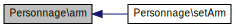
\includegraphics[width=310pt]{class_personnage_afa3847dccf10793b4512467e6fdb98fc_icgraph}
\end{center}
\end{figure}
\mbox{\Hypertarget{class_personnage_a54f0e416a628b1b7246f3c3a7c2081fa}\label{class_personnage_a54f0e416a628b1b7246f3c3a7c2081fa}} 
\index{Personnage@{Personnage}!atout@{atout}}
\index{atout@{atout}!Personnage@{Personnage}}
\subsubsection{\texorpdfstring{atout()}{atout()}}
{\footnotesize\ttfamily Personnage\+::atout (\begin{DoxyParamCaption}{ }\end{DoxyParamCaption})}



Définition à la ligne 195 du fichier Personnage.\+php.

Voici le graphe des appelants de cette fonction \+:\nopagebreak
\begin{figure}[H]
\begin{center}
\leavevmode
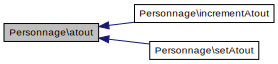
\includegraphics[width=350pt]{class_personnage_a54f0e416a628b1b7246f3c3a7c2081fa_icgraph}
\end{center}
\end{figure}
\mbox{\Hypertarget{class_personnage_a6d94c6fd714c9e8ef344e386f16c671a}\label{class_personnage_a6d94c6fd714c9e8ef344e386f16c671a}} 
\index{Personnage@{Personnage}!att@{att}}
\index{att@{att}!Personnage@{Personnage}}
\subsubsection{\texorpdfstring{att()}{att()}}
{\footnotesize\ttfamily Personnage\+::att (\begin{DoxyParamCaption}{ }\end{DoxyParamCaption})}



Définition à la ligne 216 du fichier Personnage.\+php.

Voici le graphe des appelants de cette fonction \+:\nopagebreak
\begin{figure}[H]
\begin{center}
\leavevmode
\includegraphics[width=298pt]{class_personnage_a6d94c6fd714c9e8ef344e386f16c671a_icgraph}
\end{center}
\end{figure}
\mbox{\Hypertarget{class_personnage_ae91b38c8dfaceca0eda40ae2ea66b99d}\label{class_personnage_ae91b38c8dfaceca0eda40ae2ea66b99d}} 
\index{Personnage@{Personnage}!crit@{crit}}
\index{crit@{crit}!Personnage@{Personnage}}
\subsubsection{\texorpdfstring{crit()}{crit()}}
{\footnotesize\ttfamily Personnage\+::crit (\begin{DoxyParamCaption}{ }\end{DoxyParamCaption})}



Définition à la ligne 205 du fichier Personnage.\+php.

Voici le graphe des appelants de cette fonction \+:\nopagebreak
\begin{figure}[H]
\begin{center}
\leavevmode
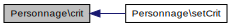
\includegraphics[width=304pt]{class_personnage_ae91b38c8dfaceca0eda40ae2ea66b99d_icgraph}
\end{center}
\end{figure}
\mbox{\Hypertarget{class_personnage_a570935e88aa03fb191a3f06a41f5aec5}\label{class_personnage_a570935e88aa03fb191a3f06a41f5aec5}} 
\index{Personnage@{Personnage}!debut\+\_\+combat@{debut\+\_\+combat}}
\index{debut\+\_\+combat@{debut\+\_\+combat}!Personnage@{Personnage}}
\subsubsection{\texorpdfstring{debut\+\_\+combat()}{debut\_combat()}}
{\footnotesize\ttfamily Personnage\+::debut\+\_\+combat (\begin{DoxyParamCaption}{ }\end{DoxyParamCaption})}



Définition à la ligne 163 du fichier Personnage.\+php.

Voici le graphe d\textquotesingle{}appel pour cette fonction \+:\nopagebreak
\begin{figure}[H]
\begin{center}
\leavevmode
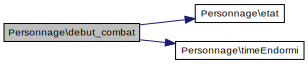
\includegraphics[width=350pt]{class_personnage_a570935e88aa03fb191a3f06a41f5aec5_cgraph}
\end{center}
\end{figure}
\mbox{\Hypertarget{class_personnage_adcc095fcc5f137e90860386b4b977817}\label{class_personnage_adcc095fcc5f137e90860386b4b977817}} 
\index{Personnage@{Personnage}!def@{def}}
\index{def@{def}!Personnage@{Personnage}}
\subsubsection{\texorpdfstring{def()}{def()}}
{\footnotesize\ttfamily Personnage\+::def (\begin{DoxyParamCaption}{ }\end{DoxyParamCaption})}



Définition à la ligne 199 du fichier Personnage.\+php.

Voici le graphe des appelants de cette fonction \+:\nopagebreak
\begin{figure}[H]
\begin{center}
\leavevmode
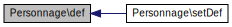
\includegraphics[width=304pt]{class_personnage_adcc095fcc5f137e90860386b4b977817_icgraph}
\end{center}
\end{figure}
\mbox{\Hypertarget{class_personnage_a7c3150644dfeedeae54ca86e43bc29a0}\label{class_personnage_a7c3150644dfeedeae54ca86e43bc29a0}} 
\index{Personnage@{Personnage}!emp\+\_\+team@{emp\+\_\+team}}
\index{emp\+\_\+team@{emp\+\_\+team}!Personnage@{Personnage}}
\subsubsection{\texorpdfstring{emp\+\_\+team()}{emp\_team()}}
{\footnotesize\ttfamily Personnage\+::emp\+\_\+team (\begin{DoxyParamCaption}{ }\end{DoxyParamCaption})}



Définition à la ligne 217 du fichier Personnage.\+php.

Voici le graphe des appelants de cette fonction \+:\nopagebreak
\begin{figure}[H]
\begin{center}
\leavevmode
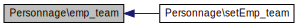
\includegraphics[width=350pt]{class_personnage_a7c3150644dfeedeae54ca86e43bc29a0_icgraph}
\end{center}
\end{figure}
\mbox{\Hypertarget{class_personnage_aae5ecffa3c0802af6664ad0f3b396561}\label{class_personnage_aae5ecffa3c0802af6664ad0f3b396561}} 
\index{Personnage@{Personnage}!esc@{esc}}
\index{esc@{esc}!Personnage@{Personnage}}
\subsubsection{\texorpdfstring{esc()}{esc()}}
{\footnotesize\ttfamily Personnage\+::esc (\begin{DoxyParamCaption}{ }\end{DoxyParamCaption})}



Définition à la ligne 204 du fichier Personnage.\+php.

Voici le graphe des appelants de cette fonction \+:\nopagebreak
\begin{figure}[H]
\begin{center}
\leavevmode
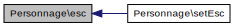
\includegraphics[width=307pt]{class_personnage_aae5ecffa3c0802af6664ad0f3b396561_icgraph}
\end{center}
\end{figure}
\mbox{\Hypertarget{class_personnage_aabf0bcd80fcea089de16f33c029aae12}\label{class_personnage_aabf0bcd80fcea089de16f33c029aae12}} 
\index{Personnage@{Personnage}!est\+Endormi@{est\+Endormi}}
\index{est\+Endormi@{est\+Endormi}!Personnage@{Personnage}}
\subsubsection{\texorpdfstring{est\+Endormi()}{estEndormi()}}
{\footnotesize\ttfamily Personnage\+::est\+Endormi (\begin{DoxyParamCaption}{ }\end{DoxyParamCaption})}



Définition à la ligne 80 du fichier Personnage.\+php.

Voici le graphe d\textquotesingle{}appel pour cette fonction \+:\nopagebreak
\begin{figure}[H]
\begin{center}
\leavevmode
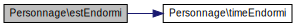
\includegraphics[width=350pt]{class_personnage_aabf0bcd80fcea089de16f33c029aae12_cgraph}
\end{center}
\end{figure}
Voici le graphe des appelants de cette fonction \+:\nopagebreak
\begin{figure}[H]
\begin{center}
\leavevmode
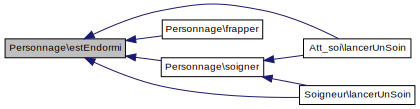
\includegraphics[width=350pt]{class_personnage_aabf0bcd80fcea089de16f33c029aae12_icgraph}
\end{center}
\end{figure}
\mbox{\Hypertarget{class_personnage_addeceec710baf3ae687f36151bc5def4}\label{class_personnage_addeceec710baf3ae687f36151bc5def4}} 
\index{Personnage@{Personnage}!etat@{etat}}
\index{etat@{etat}!Personnage@{Personnage}}
\subsubsection{\texorpdfstring{etat()}{etat()}}
{\footnotesize\ttfamily Personnage\+::etat (\begin{DoxyParamCaption}{ }\end{DoxyParamCaption})}



Définition à la ligne 208 du fichier Personnage.\+php.

Voici le graphe des appelants de cette fonction \+:\nopagebreak
\begin{figure}[H]
\begin{center}
\leavevmode
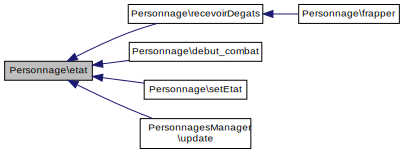
\includegraphics[width=350pt]{class_personnage_addeceec710baf3ae687f36151bc5def4_icgraph}
\end{center}
\end{figure}
\mbox{\Hypertarget{class_personnage_ade67f55b78368cd7e3c92128bb7ae67d}\label{class_personnage_ade67f55b78368cd7e3c92128bb7ae67d}} 
\index{Personnage@{Personnage}!etoile@{etoile}}
\index{etoile@{etoile}!Personnage@{Personnage}}
\subsubsection{\texorpdfstring{etoile()}{etoile()}}
{\footnotesize\ttfamily Personnage\+::etoile (\begin{DoxyParamCaption}{ }\end{DoxyParamCaption})}



Définition à la ligne 194 du fichier Personnage.\+php.

Voici le graphe des appelants de cette fonction \+:\nopagebreak
\begin{figure}[H]
\begin{center}
\leavevmode
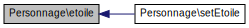
\includegraphics[width=324pt]{class_personnage_ade67f55b78368cd7e3c92128bb7ae67d_icgraph}
\end{center}
\end{figure}
\mbox{\Hypertarget{class_personnage_a1deaeddff5bc8766d52da4fc2d0b8032}\label{class_personnage_a1deaeddff5bc8766d52da4fc2d0b8032}} 
\index{Personnage@{Personnage}!frapper@{frapper}}
\index{frapper@{frapper}!Personnage@{Personnage}}
\subsubsection{\texorpdfstring{frapper()}{frapper()}}
{\footnotesize\ttfamily Personnage\+::frapper (\begin{DoxyParamCaption}\item[{\mbox{\hyperlink{class_personnage}{Personnage}}}]{\$perso,  }\item[{\mbox{\hyperlink{class_personnage}{Personnage}}}]{\$perso2 }\end{DoxyParamCaption})}



Fonction pour frapper. 

Fonction permettant à un personnage de frapper un autre personnage. S\textquotesingle{}il est sa propre cible ou s\textquotesingle{}il est endormit, il ne pourra pas frapper 
\begin{DoxyParams}[1]{Paramètres}
\mbox{\hyperlink{class_personnage}{Personnage}} & {\em \$perso} & Perso qui se fait frapper. \\
\hline
\mbox{\hyperlink{class_personnage}{Personnage}} & {\em \$perso2} & Person qui frappe. \\
\hline
\end{DoxyParams}
\begin{DoxyReturn}{Renvoie}
Renvoie à la fonction qui permet de recevoir des dégats (\char`\"{}recevoir\+Degats()\char`\"{}). 
\end{DoxyReturn}


Définition à la ligne 93 du fichier Personnage.\+php.

Voici le graphe d\textquotesingle{}appel pour cette fonction \+:\nopagebreak
\begin{figure}[H]
\begin{center}
\leavevmode
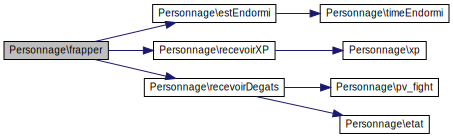
\includegraphics[width=350pt]{class_personnage_a1deaeddff5bc8766d52da4fc2d0b8032_cgraph}
\end{center}
\end{figure}
\mbox{\Hypertarget{class_personnage_ae95e51cac2f518a6a38d025f5580be3f}\label{class_personnage_ae95e51cac2f518a6a38d025f5580be3f}} 
\index{Personnage@{Personnage}!hydrate@{hydrate}}
\index{hydrate@{hydrate}!Personnage@{Personnage}}
\subsubsection{\texorpdfstring{hydrate()}{hydrate()}}
{\footnotesize\ttfamily Personnage\+::hydrate (\begin{DoxyParamCaption}\item[{array}]{\$donnees }\end{DoxyParamCaption})}



Définition à la ligne 64 du fichier Personnage.\+php.

Voici le graphe des appelants de cette fonction \+:\nopagebreak
\begin{figure}[H]
\begin{center}
\leavevmode
\includegraphics[width=346pt]{class_personnage_ae95e51cac2f518a6a38d025f5580be3f_icgraph}
\end{center}
\end{figure}
\mbox{\Hypertarget{class_personnage_aa34eed6a48eb3734596505b58497f2f1}\label{class_personnage_aa34eed6a48eb3734596505b58497f2f1}} 
\index{Personnage@{Personnage}!id\+\_\+perso@{id\+\_\+perso}}
\index{id\+\_\+perso@{id\+\_\+perso}!Personnage@{Personnage}}
\subsubsection{\texorpdfstring{id\+\_\+perso()}{id\_perso()}}
{\footnotesize\ttfamily Personnage\+::id\+\_\+perso (\begin{DoxyParamCaption}{ }\end{DoxyParamCaption})}



Définition à la ligne 189 du fichier Personnage.\+php.

Voici le graphe des appelants de cette fonction \+:\nopagebreak
\begin{figure}[H]
\begin{center}
\leavevmode
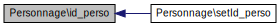
\includegraphics[width=350pt]{class_personnage_aa34eed6a48eb3734596505b58497f2f1_icgraph}
\end{center}
\end{figure}
\mbox{\Hypertarget{class_personnage_ab0fc8802437d3f7bbc0da720597d0393}\label{class_personnage_ab0fc8802437d3f7bbc0da720597d0393}} 
\index{Personnage@{Personnage}!id\+\_\+persos@{id\+\_\+persos}}
\index{id\+\_\+persos@{id\+\_\+persos}!Personnage@{Personnage}}
\subsubsection{\texorpdfstring{id\+\_\+persos()}{id\_persos()}}
{\footnotesize\ttfamily Personnage\+::id\+\_\+persos (\begin{DoxyParamCaption}{ }\end{DoxyParamCaption})}



Définition à la ligne 210 du fichier Personnage.\+php.

Voici le graphe des appelants de cette fonction \+:\nopagebreak
\begin{figure}[H]
\begin{center}
\leavevmode
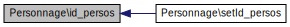
\includegraphics[width=350pt]{class_personnage_ab0fc8802437d3f7bbc0da720597d0393_icgraph}
\end{center}
\end{figure}
\mbox{\Hypertarget{class_personnage_a83ccdd40630a166b7a1f5c84dd742e8c}\label{class_personnage_a83ccdd40630a166b7a1f5c84dd742e8c}} 
\index{Personnage@{Personnage}!id\+\_\+user@{id\+\_\+user}}
\index{id\+\_\+user@{id\+\_\+user}!Personnage@{Personnage}}
\subsubsection{\texorpdfstring{id\+\_\+user()}{id\_user()}}
{\footnotesize\ttfamily Personnage\+::id\+\_\+user (\begin{DoxyParamCaption}{ }\end{DoxyParamCaption})}



Définition à la ligne 188 du fichier Personnage.\+php.

Voici le graphe des appelants de cette fonction \+:\nopagebreak
\begin{figure}[H]
\begin{center}
\leavevmode
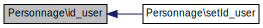
\includegraphics[width=341pt]{class_personnage_a83ccdd40630a166b7a1f5c84dd742e8c_icgraph}
\end{center}
\end{figure}
\mbox{\Hypertarget{class_personnage_a744674b144008a43e37036344accb378}\label{class_personnage_a744674b144008a43e37036344accb378}} 
\index{Personnage@{Personnage}!increment\+Atout@{increment\+Atout}}
\index{increment\+Atout@{increment\+Atout}!Personnage@{Personnage}}
\subsubsection{\texorpdfstring{increment\+Atout()}{incrementAtout()}}
{\footnotesize\ttfamily Personnage\+::increment\+Atout (\begin{DoxyParamCaption}{ }\end{DoxyParamCaption})}



Définition à la ligne 175 du fichier Personnage.\+php.

Voici le graphe d\textquotesingle{}appel pour cette fonction \+:\nopagebreak
\begin{figure}[H]
\begin{center}
\leavevmode
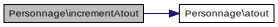
\includegraphics[width=350pt]{class_personnage_a744674b144008a43e37036344accb378_cgraph}
\end{center}
\end{figure}
\mbox{\Hypertarget{class_personnage_a061130b0c1c551d893ecffff2553cb93}\label{class_personnage_a061130b0c1c551d893ecffff2553cb93}} 
\index{Personnage@{Personnage}!niveau@{niveau}}
\index{niveau@{niveau}!Personnage@{Personnage}}
\subsubsection{\texorpdfstring{niveau()}{niveau()}}
{\footnotesize\ttfamily Personnage\+::niveau (\begin{DoxyParamCaption}{ }\end{DoxyParamCaption})}



Définition à la ligne 192 du fichier Personnage.\+php.

Voici le graphe des appelants de cette fonction \+:\nopagebreak
\begin{figure}[H]
\begin{center}
\leavevmode
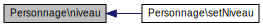
\includegraphics[width=350pt]{class_personnage_a061130b0c1c551d893ecffff2553cb93_icgraph}
\end{center}
\end{figure}
\mbox{\Hypertarget{class_personnage_a236eb0f89c6676425ddfcc25967a527a}\label{class_personnage_a236eb0f89c6676425ddfcc25967a527a}} 
\index{Personnage@{Personnage}!nom@{nom}}
\index{nom@{nom}!Personnage@{Personnage}}
\subsubsection{\texorpdfstring{nom()}{nom()}}
{\footnotesize\ttfamily Personnage\+::nom (\begin{DoxyParamCaption}{ }\end{DoxyParamCaption})}



Définition à la ligne 209 du fichier Personnage.\+php.

Voici le graphe des appelants de cette fonction \+:\nopagebreak
\begin{figure}[H]
\begin{center}
\leavevmode
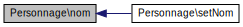
\includegraphics[width=315pt]{class_personnage_a236eb0f89c6676425ddfcc25967a527a_icgraph}
\end{center}
\end{figure}
\mbox{\Hypertarget{class_personnage_a4c3db78c974d2b3d0345a677e1370162}\label{class_personnage_a4c3db78c974d2b3d0345a677e1370162}} 
\index{Personnage@{Personnage}!pen@{pen}}
\index{pen@{pen}!Personnage@{Personnage}}
\subsubsection{\texorpdfstring{pen()}{pen()}}
{\footnotesize\ttfamily Personnage\+::pen (\begin{DoxyParamCaption}{ }\end{DoxyParamCaption})}



Définition à la ligne 201 du fichier Personnage.\+php.

Voici le graphe des appelants de cette fonction \+:\nopagebreak
\begin{figure}[H]
\begin{center}
\leavevmode
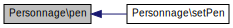
\includegraphics[width=309pt]{class_personnage_a4c3db78c974d2b3d0345a677e1370162_icgraph}
\end{center}
\end{figure}
\mbox{\Hypertarget{class_personnage_ae7675cda70f8e9488d1b4e28550a0871}\label{class_personnage_ae7675cda70f8e9488d1b4e28550a0871}} 
\index{Personnage@{Personnage}!pre@{pre}}
\index{pre@{pre}!Personnage@{Personnage}}
\subsubsection{\texorpdfstring{pre()}{pre()}}
{\footnotesize\ttfamily Personnage\+::pre (\begin{DoxyParamCaption}{ }\end{DoxyParamCaption})}



Définition à la ligne 203 du fichier Personnage.\+php.

Voici le graphe des appelants de cette fonction \+:\nopagebreak
\begin{figure}[H]
\begin{center}
\leavevmode
\includegraphics[width=305pt]{class_personnage_ae7675cda70f8e9488d1b4e28550a0871_icgraph}
\end{center}
\end{figure}
\mbox{\Hypertarget{class_personnage_ac33d3de759181a59960066291c8065a9}\label{class_personnage_ac33d3de759181a59960066291c8065a9}} 
\index{Personnage@{Personnage}!pv@{pv}}
\index{pv@{pv}!Personnage@{Personnage}}
\subsubsection{\texorpdfstring{pv()}{pv()}}
{\footnotesize\ttfamily Personnage\+::pv (\begin{DoxyParamCaption}{ }\end{DoxyParamCaption})}



Définition à la ligne 215 du fichier Personnage.\+php.

Voici le graphe des appelants de cette fonction \+:\nopagebreak
\begin{figure}[H]
\begin{center}
\leavevmode
\includegraphics[width=297pt]{class_personnage_ac33d3de759181a59960066291c8065a9_icgraph}
\end{center}
\end{figure}
\mbox{\Hypertarget{class_personnage_ae8daf1e07c298cf03a98b6b06d3adfd9}\label{class_personnage_ae8daf1e07c298cf03a98b6b06d3adfd9}} 
\index{Personnage@{Personnage}!qualite@{qualite}}
\index{qualite@{qualite}!Personnage@{Personnage}}
\subsubsection{\texorpdfstring{qualite()}{qualite()}}
{\footnotesize\ttfamily Personnage\+::qualite (\begin{DoxyParamCaption}{ }\end{DoxyParamCaption})}



Définition à la ligne 193 du fichier Personnage.\+php.

Voici le graphe des appelants de cette fonction \+:\nopagebreak
\begin{figure}[H]
\begin{center}
\leavevmode
\includegraphics[width=336pt]{class_personnage_ae8daf1e07c298cf03a98b6b06d3adfd9_icgraph}
\end{center}
\end{figure}
\mbox{\Hypertarget{class_personnage_a226affce78dca0151e0901896e58f14d}\label{class_personnage_a226affce78dca0151e0901896e58f14d}} 
\index{Personnage@{Personnage}!recevoir\+Degats@{recevoir\+Degats}}
\index{recevoir\+Degats@{recevoir\+Degats}!Personnage@{Personnage}}
\subsubsection{\texorpdfstring{recevoir\+Degats()}{recevoirDegats()}}
{\footnotesize\ttfamily Personnage\+::recevoir\+Degats (\begin{DoxyParamCaption}\item[{}]{\$perso2 }\end{DoxyParamCaption})}



Définition à la ligne 123 du fichier Personnage.\+php.

Voici le graphe d\textquotesingle{}appel pour cette fonction \+:\nopagebreak
\begin{figure}[H]
\begin{center}
\leavevmode
\includegraphics[width=345pt]{class_personnage_a226affce78dca0151e0901896e58f14d_cgraph}
\end{center}
\end{figure}
Voici le graphe des appelants de cette fonction \+:\nopagebreak
\begin{figure}[H]
\begin{center}
\leavevmode
\includegraphics[width=350pt]{class_personnage_a226affce78dca0151e0901896e58f14d_icgraph}
\end{center}
\end{figure}
\mbox{\Hypertarget{class_personnage_acadb61228a3ebdf18318771f954e2ae0}\label{class_personnage_acadb61228a3ebdf18318771f954e2ae0}} 
\index{Personnage@{Personnage}!recevoir\+Soins@{recevoir\+Soins}}
\index{recevoir\+Soins@{recevoir\+Soins}!Personnage@{Personnage}}
\subsubsection{\texorpdfstring{recevoir\+Soins()}{recevoirSoins()}}
{\footnotesize\ttfamily Personnage\+::recevoir\+Soins (\begin{DoxyParamCaption}\item[{}]{\$perso }\end{DoxyParamCaption})}



Définition à la ligne 152 du fichier Personnage.\+php.

\mbox{\Hypertarget{class_personnage_aa64edf7d4c080193213b12643eb05a5d}\label{class_personnage_aa64edf7d4c080193213b12643eb05a5d}} 
\index{Personnage@{Personnage}!recevoir\+XP@{recevoir\+XP}}
\index{recevoir\+XP@{recevoir\+XP}!Personnage@{Personnage}}
\subsubsection{\texorpdfstring{recevoir\+X\+P()}{recevoirXP()}}
{\footnotesize\ttfamily Personnage\+::recevoir\+XP (\begin{DoxyParamCaption}\item[{}]{\$val }\end{DoxyParamCaption})}



Définition à la ligne 111 du fichier Personnage.\+php.

Voici le graphe d\textquotesingle{}appel pour cette fonction \+:\nopagebreak
\begin{figure}[H]
\begin{center}
\leavevmode
\includegraphics[width=345pt]{class_personnage_aa64edf7d4c080193213b12643eb05a5d_cgraph}
\end{center}
\end{figure}
Voici le graphe des appelants de cette fonction \+:\nopagebreak
\begin{figure}[H]
\begin{center}
\leavevmode
\includegraphics[width=350pt]{class_personnage_aa64edf7d4c080193213b12643eb05a5d_icgraph}
\end{center}
\end{figure}
\mbox{\Hypertarget{class_personnage_ab0503fe49e1a5403fe6d43d7d424e3ef}\label{class_personnage_ab0503fe49e1a5403fe6d43d7d424e3ef}} 
\index{Personnage@{Personnage}!reveil@{reveil}}
\index{reveil@{reveil}!Personnage@{Personnage}}
\subsubsection{\texorpdfstring{reveil()}{reveil()}}
{\footnotesize\ttfamily Personnage\+::reveil (\begin{DoxyParamCaption}{ }\end{DoxyParamCaption})}



Définition à la ligne 170 du fichier Personnage.\+php.

Voici le graphe d\textquotesingle{}appel pour cette fonction \+:\nopagebreak
\begin{figure}[H]
\begin{center}
\leavevmode
\includegraphics[width=341pt]{class_personnage_ab0503fe49e1a5403fe6d43d7d424e3ef_cgraph}
\end{center}
\end{figure}
\mbox{\Hypertarget{class_personnage_aed5fd24acaa0244d3bafd595b8492507}\label{class_personnage_aed5fd24acaa0244d3bafd595b8492507}} 
\index{Personnage@{Personnage}!set\+Arm@{set\+Arm}}
\index{set\+Arm@{set\+Arm}!Personnage@{Personnage}}
\subsubsection{\texorpdfstring{set\+Arm()}{setArm()}}
{\footnotesize\ttfamily Personnage\+::set\+Arm (\begin{DoxyParamCaption}\item[{}]{\$arm }\end{DoxyParamCaption})}



Définition à la ligne 343 du fichier Personnage.\+php.

Voici le graphe d\textquotesingle{}appel pour cette fonction \+:\nopagebreak
\begin{figure}[H]
\begin{center}
\leavevmode
\includegraphics[width=310pt]{class_personnage_aed5fd24acaa0244d3bafd595b8492507_cgraph}
\end{center}
\end{figure}
\mbox{\Hypertarget{class_personnage_a3ba4e51f81e8d865675c1514332c0ac5}\label{class_personnage_a3ba4e51f81e8d865675c1514332c0ac5}} 
\index{Personnage@{Personnage}!set\+Atout@{set\+Atout}}
\index{set\+Atout@{set\+Atout}!Personnage@{Personnage}}
\subsubsection{\texorpdfstring{set\+Atout()}{setAtout()}}
{\footnotesize\ttfamily Personnage\+::set\+Atout (\begin{DoxyParamCaption}\item[{}]{\$atout }\end{DoxyParamCaption})}



Définition à la ligne 219 du fichier Personnage.\+php.

Voici le graphe d\textquotesingle{}appel pour cette fonction \+:\nopagebreak
\begin{figure}[H]
\begin{center}
\leavevmode
\includegraphics[width=320pt]{class_personnage_a3ba4e51f81e8d865675c1514332c0ac5_cgraph}
\end{center}
\end{figure}
\mbox{\Hypertarget{class_personnage_a7b007c31486eff8234acabe91d6d1244}\label{class_personnage_a7b007c31486eff8234acabe91d6d1244}} 
\index{Personnage@{Personnage}!set\+Att@{set\+Att}}
\index{set\+Att@{set\+Att}!Personnage@{Personnage}}
\subsubsection{\texorpdfstring{set\+Att()}{setAtt()}}
{\footnotesize\ttfamily Personnage\+::set\+Att (\begin{DoxyParamCaption}\item[{}]{\$att }\end{DoxyParamCaption})}



Définition à la ligne 441 du fichier Personnage.\+php.

Voici le graphe d\textquotesingle{}appel pour cette fonction \+:\nopagebreak
\begin{figure}[H]
\begin{center}
\leavevmode
\includegraphics[width=298pt]{class_personnage_a7b007c31486eff8234acabe91d6d1244_cgraph}
\end{center}
\end{figure}
\mbox{\Hypertarget{class_personnage_a5caf7c4c695a03b2d5ade3ec5963d749}\label{class_personnage_a5caf7c4c695a03b2d5ade3ec5963d749}} 
\index{Personnage@{Personnage}!set\+Crit@{set\+Crit}}
\index{set\+Crit@{set\+Crit}!Personnage@{Personnage}}
\subsubsection{\texorpdfstring{set\+Crit()}{setCrit()}}
{\footnotesize\ttfamily Personnage\+::set\+Crit (\begin{DoxyParamCaption}\item[{}]{\$crit }\end{DoxyParamCaption})}



Définition à la ligne 376 du fichier Personnage.\+php.

Voici le graphe d\textquotesingle{}appel pour cette fonction \+:\nopagebreak
\begin{figure}[H]
\begin{center}
\leavevmode
\includegraphics[width=304pt]{class_personnage_a5caf7c4c695a03b2d5ade3ec5963d749_cgraph}
\end{center}
\end{figure}
\mbox{\Hypertarget{class_personnage_abe66826f9e8f8764566fcebc25bdb080}\label{class_personnage_abe66826f9e8f8764566fcebc25bdb080}} 
\index{Personnage@{Personnage}!set\+Def@{set\+Def}}
\index{set\+Def@{set\+Def}!Personnage@{Personnage}}
\subsubsection{\texorpdfstring{set\+Def()}{setDef()}}
{\footnotesize\ttfamily Personnage\+::set\+Def (\begin{DoxyParamCaption}\item[{}]{\$def }\end{DoxyParamCaption})}



Définition à la ligne 310 du fichier Personnage.\+php.

Voici le graphe d\textquotesingle{}appel pour cette fonction \+:\nopagebreak
\begin{figure}[H]
\begin{center}
\leavevmode
\includegraphics[width=304pt]{class_personnage_abe66826f9e8f8764566fcebc25bdb080_cgraph}
\end{center}
\end{figure}
\mbox{\Hypertarget{class_personnage_aec0f318abc45dee8a4b011722efd74ed}\label{class_personnage_aec0f318abc45dee8a4b011722efd74ed}} 
\index{Personnage@{Personnage}!set\+Emp\+\_\+team@{set\+Emp\+\_\+team}}
\index{set\+Emp\+\_\+team@{set\+Emp\+\_\+team}!Personnage@{Personnage}}
\subsubsection{\texorpdfstring{set\+Emp\+\_\+team()}{setEmp\_team()}}
{\footnotesize\ttfamily Personnage\+::set\+Emp\+\_\+team (\begin{DoxyParamCaption}\item[{}]{\$emp\+\_\+team }\end{DoxyParamCaption})}



Définition à la ligne 452 du fichier Personnage.\+php.

Voici le graphe d\textquotesingle{}appel pour cette fonction \+:\nopagebreak
\begin{figure}[H]
\begin{center}
\leavevmode
\includegraphics[width=350pt]{class_personnage_aec0f318abc45dee8a4b011722efd74ed_cgraph}
\end{center}
\end{figure}
\mbox{\Hypertarget{class_personnage_aefa2ea9bcc007c36688272ef5881e30a}\label{class_personnage_aefa2ea9bcc007c36688272ef5881e30a}} 
\index{Personnage@{Personnage}!set\+Esc@{set\+Esc}}
\index{set\+Esc@{set\+Esc}!Personnage@{Personnage}}
\subsubsection{\texorpdfstring{set\+Esc()}{setEsc()}}
{\footnotesize\ttfamily Personnage\+::set\+Esc (\begin{DoxyParamCaption}\item[{}]{\$esc }\end{DoxyParamCaption})}



Définition à la ligne 365 du fichier Personnage.\+php.

Voici le graphe d\textquotesingle{}appel pour cette fonction \+:\nopagebreak
\begin{figure}[H]
\begin{center}
\leavevmode
\includegraphics[width=307pt]{class_personnage_aefa2ea9bcc007c36688272ef5881e30a_cgraph}
\end{center}
\end{figure}
\mbox{\Hypertarget{class_personnage_af368ea425266209c0dcf800bdfcf1b84}\label{class_personnage_af368ea425266209c0dcf800bdfcf1b84}} 
\index{Personnage@{Personnage}!set\+Etat@{set\+Etat}}
\index{set\+Etat@{set\+Etat}!Personnage@{Personnage}}
\subsubsection{\texorpdfstring{set\+Etat()}{setEtat()}}
{\footnotesize\ttfamily Personnage\+::set\+Etat (\begin{DoxyParamCaption}\item[{}]{\$etat }\end{DoxyParamCaption})}



Définition à la ligne 409 du fichier Personnage.\+php.

Voici le graphe d\textquotesingle{}appel pour cette fonction \+:\nopagebreak
\begin{figure}[H]
\begin{center}
\leavevmode
\includegraphics[width=309pt]{class_personnage_af368ea425266209c0dcf800bdfcf1b84_cgraph}
\end{center}
\end{figure}
\mbox{\Hypertarget{class_personnage_ad45b2c2c30828e3f0e56d563c031235d}\label{class_personnage_ad45b2c2c30828e3f0e56d563c031235d}} 
\index{Personnage@{Personnage}!set\+Etoile@{set\+Etoile}}
\index{set\+Etoile@{set\+Etoile}!Personnage@{Personnage}}
\subsubsection{\texorpdfstring{set\+Etoile()}{setEtoile()}}
{\footnotesize\ttfamily Personnage\+::set\+Etoile (\begin{DoxyParamCaption}\item[{}]{\$etoile }\end{DoxyParamCaption})}



Définition à la ligne 241 du fichier Personnage.\+php.

Voici le graphe d\textquotesingle{}appel pour cette fonction \+:\nopagebreak
\begin{figure}[H]
\begin{center}
\leavevmode
\includegraphics[width=324pt]{class_personnage_ad45b2c2c30828e3f0e56d563c031235d_cgraph}
\end{center}
\end{figure}
\mbox{\Hypertarget{class_personnage_abcc3bdc5236dbfccd50c3dc5db1e8fce}\label{class_personnage_abcc3bdc5236dbfccd50c3dc5db1e8fce}} 
\index{Personnage@{Personnage}!set\+Id\+\_\+perso@{set\+Id\+\_\+perso}}
\index{set\+Id\+\_\+perso@{set\+Id\+\_\+perso}!Personnage@{Personnage}}
\subsubsection{\texorpdfstring{set\+Id\+\_\+perso()}{setId\_perso()}}
{\footnotesize\ttfamily Personnage\+::set\+Id\+\_\+perso (\begin{DoxyParamCaption}\item[{}]{\$id\+\_\+perso }\end{DoxyParamCaption})}



Définition à la ligne 235 du fichier Personnage.\+php.

Voici le graphe d\textquotesingle{}appel pour cette fonction \+:\nopagebreak
\begin{figure}[H]
\begin{center}
\leavevmode
\includegraphics[width=350pt]{class_personnage_abcc3bdc5236dbfccd50c3dc5db1e8fce_cgraph}
\end{center}
\end{figure}
\mbox{\Hypertarget{class_personnage_ac11963514b5d9911283b7ff61e094125}\label{class_personnage_ac11963514b5d9911283b7ff61e094125}} 
\index{Personnage@{Personnage}!set\+Id\+\_\+persos@{set\+Id\+\_\+persos}}
\index{set\+Id\+\_\+persos@{set\+Id\+\_\+persos}!Personnage@{Personnage}}
\subsubsection{\texorpdfstring{set\+Id\+\_\+persos()}{setId\_persos()}}
{\footnotesize\ttfamily Personnage\+::set\+Id\+\_\+persos (\begin{DoxyParamCaption}\item[{}]{\$id\+\_\+persos }\end{DoxyParamCaption})}



Définition à la ligne 414 du fichier Personnage.\+php.

Voici le graphe d\textquotesingle{}appel pour cette fonction \+:\nopagebreak
\begin{figure}[H]
\begin{center}
\leavevmode
\includegraphics[width=350pt]{class_personnage_ac11963514b5d9911283b7ff61e094125_cgraph}
\end{center}
\end{figure}
\mbox{\Hypertarget{class_personnage_abe08b8cf03683f5a0f577ff7f1ac88f2}\label{class_personnage_abe08b8cf03683f5a0f577ff7f1ac88f2}} 
\index{Personnage@{Personnage}!set\+Id\+\_\+user@{set\+Id\+\_\+user}}
\index{set\+Id\+\_\+user@{set\+Id\+\_\+user}!Personnage@{Personnage}}
\subsubsection{\texorpdfstring{set\+Id\+\_\+user()}{setId\_user()}}
{\footnotesize\ttfamily Personnage\+::set\+Id\+\_\+user (\begin{DoxyParamCaption}\item[{}]{\$id\+\_\+user }\end{DoxyParamCaption})}



Définition à la ligne 229 du fichier Personnage.\+php.

Voici le graphe d\textquotesingle{}appel pour cette fonction \+:\nopagebreak
\begin{figure}[H]
\begin{center}
\leavevmode
\includegraphics[width=341pt]{class_personnage_abe08b8cf03683f5a0f577ff7f1ac88f2_cgraph}
\end{center}
\end{figure}
\mbox{\Hypertarget{class_personnage_a309bc50e0ac35a942d8ffceb5a4556a9}\label{class_personnage_a309bc50e0ac35a942d8ffceb5a4556a9}} 
\index{Personnage@{Personnage}!set\+Niveau@{set\+Niveau}}
\index{set\+Niveau@{set\+Niveau}!Personnage@{Personnage}}
\subsubsection{\texorpdfstring{set\+Niveau()}{setNiveau()}}
{\footnotesize\ttfamily Personnage\+::set\+Niveau (\begin{DoxyParamCaption}\item[{}]{\$niveau }\end{DoxyParamCaption})}



Définition à la ligne 275 du fichier Personnage.\+php.

Voici le graphe d\textquotesingle{}appel pour cette fonction \+:\nopagebreak
\begin{figure}[H]
\begin{center}
\leavevmode
\includegraphics[width=335pt]{class_personnage_a309bc50e0ac35a942d8ffceb5a4556a9_cgraph}
\end{center}
\end{figure}
\mbox{\Hypertarget{class_personnage_adb31f60912f384e0de79497f9128d549}\label{class_personnage_adb31f60912f384e0de79497f9128d549}} 
\index{Personnage@{Personnage}!set\+Nom@{set\+Nom}}
\index{set\+Nom@{set\+Nom}!Personnage@{Personnage}}
\subsubsection{\texorpdfstring{set\+Nom()}{setNom()}}
{\footnotesize\ttfamily Personnage\+::set\+Nom (\begin{DoxyParamCaption}\item[{}]{\$nom }\end{DoxyParamCaption})}



Définition à la ligne 420 du fichier Personnage.\+php.

Voici le graphe d\textquotesingle{}appel pour cette fonction \+:\nopagebreak
\begin{figure}[H]
\begin{center}
\leavevmode
\includegraphics[width=315pt]{class_personnage_adb31f60912f384e0de79497f9128d549_cgraph}
\end{center}
\end{figure}
\mbox{\Hypertarget{class_personnage_aeb2ef67eccbeba4a3a296895b7570359}\label{class_personnage_aeb2ef67eccbeba4a3a296895b7570359}} 
\index{Personnage@{Personnage}!set\+Pen@{set\+Pen}}
\index{set\+Pen@{set\+Pen}!Personnage@{Personnage}}
\subsubsection{\texorpdfstring{set\+Pen()}{setPen()}}
{\footnotesize\ttfamily Personnage\+::set\+Pen (\begin{DoxyParamCaption}\item[{}]{\$pen }\end{DoxyParamCaption})}



Définition à la ligne 332 du fichier Personnage.\+php.

Voici le graphe d\textquotesingle{}appel pour cette fonction \+:\nopagebreak
\begin{figure}[H]
\begin{center}
\leavevmode
\includegraphics[width=309pt]{class_personnage_aeb2ef67eccbeba4a3a296895b7570359_cgraph}
\end{center}
\end{figure}
\mbox{\Hypertarget{class_personnage_acf536edaa86c48b4385bd77841d5bc7c}\label{class_personnage_acf536edaa86c48b4385bd77841d5bc7c}} 
\index{Personnage@{Personnage}!set\+Pre@{set\+Pre}}
\index{set\+Pre@{set\+Pre}!Personnage@{Personnage}}
\subsubsection{\texorpdfstring{set\+Pre()}{setPre()}}
{\footnotesize\ttfamily Personnage\+::set\+Pre (\begin{DoxyParamCaption}\item[{}]{\$pre }\end{DoxyParamCaption})}



Définition à la ligne 354 du fichier Personnage.\+php.

Voici le graphe d\textquotesingle{}appel pour cette fonction \+:\nopagebreak
\begin{figure}[H]
\begin{center}
\leavevmode
\includegraphics[width=305pt]{class_personnage_acf536edaa86c48b4385bd77841d5bc7c_cgraph}
\end{center}
\end{figure}
\mbox{\Hypertarget{class_personnage_ab0106674504168da06bff966c9000ffb}\label{class_personnage_ab0106674504168da06bff966c9000ffb}} 
\index{Personnage@{Personnage}!set\+Pv@{set\+Pv}}
\index{set\+Pv@{set\+Pv}!Personnage@{Personnage}}
\subsubsection{\texorpdfstring{set\+Pv()}{setPv()}}
{\footnotesize\ttfamily Personnage\+::set\+Pv (\begin{DoxyParamCaption}\item[{}]{\$pv }\end{DoxyParamCaption})}



Définition à la ligne 430 du fichier Personnage.\+php.

Voici le graphe d\textquotesingle{}appel pour cette fonction \+:\nopagebreak
\begin{figure}[H]
\begin{center}
\leavevmode
\includegraphics[width=297pt]{class_personnage_ab0106674504168da06bff966c9000ffb_cgraph}
\end{center}
\end{figure}
\mbox{\Hypertarget{class_personnage_a85bad8be1af1855b0c736d84640ec820}\label{class_personnage_a85bad8be1af1855b0c736d84640ec820}} 
\index{Personnage@{Personnage}!set\+Qualite@{set\+Qualite}}
\index{set\+Qualite@{set\+Qualite}!Personnage@{Personnage}}
\subsubsection{\texorpdfstring{set\+Qualite()}{setQualite()}}
{\footnotesize\ttfamily Personnage\+::set\+Qualite (\begin{DoxyParamCaption}\item[{}]{\$qualite }\end{DoxyParamCaption})}



Définition à la ligne 265 du fichier Personnage.\+php.

Voici le graphe d\textquotesingle{}appel pour cette fonction \+:\nopagebreak
\begin{figure}[H]
\begin{center}
\leavevmode
\includegraphics[width=336pt]{class_personnage_a85bad8be1af1855b0c736d84640ec820_cgraph}
\end{center}
\end{figure}
\mbox{\Hypertarget{class_personnage_a9e07b4d56c5b54669cb6184b4b4a46c1}\label{class_personnage_a9e07b4d56c5b54669cb6184b4b4a46c1}} 
\index{Personnage@{Personnage}!set\+Soi@{set\+Soi}}
\index{set\+Soi@{set\+Soi}!Personnage@{Personnage}}
\subsubsection{\texorpdfstring{set\+Soi()}{setSoi()}}
{\footnotesize\ttfamily Personnage\+::set\+Soi (\begin{DoxyParamCaption}\item[{}]{\$soi }\end{DoxyParamCaption})}



Définition à la ligne 398 du fichier Personnage.\+php.

Voici le graphe d\textquotesingle{}appel pour cette fonction \+:\nopagebreak
\begin{figure}[H]
\begin{center}
\leavevmode
\includegraphics[width=302pt]{class_personnage_a9e07b4d56c5b54669cb6184b4b4a46c1_cgraph}
\end{center}
\end{figure}
\mbox{\Hypertarget{class_personnage_a65802b0a0d09e0d4027861542464b966}\label{class_personnage_a65802b0a0d09e0d4027861542464b966}} 
\index{Personnage@{Personnage}!set\+Stuff\+\_\+1@{set\+Stuff\+\_\+1}}
\index{set\+Stuff\+\_\+1@{set\+Stuff\+\_\+1}!Personnage@{Personnage}}
\subsubsection{\texorpdfstring{set\+Stuff\+\_\+1()}{setStuff\_1()}}
{\footnotesize\ttfamily Personnage\+::set\+Stuff\+\_\+1 (\begin{DoxyParamCaption}\item[{}]{\$stuff\+\_\+1 }\end{DoxyParamCaption})}



Définition à la ligne 463 du fichier Personnage.\+php.

Voici le graphe d\textquotesingle{}appel pour cette fonction \+:\nopagebreak
\begin{figure}[H]
\begin{center}
\leavevmode
\includegraphics[width=336pt]{class_personnage_a65802b0a0d09e0d4027861542464b966_cgraph}
\end{center}
\end{figure}
\mbox{\Hypertarget{class_personnage_abbfd017defe625b98830231b7bfa8f94}\label{class_personnage_abbfd017defe625b98830231b7bfa8f94}} 
\index{Personnage@{Personnage}!set\+Stuff\+\_\+2@{set\+Stuff\+\_\+2}}
\index{set\+Stuff\+\_\+2@{set\+Stuff\+\_\+2}!Personnage@{Personnage}}
\subsubsection{\texorpdfstring{set\+Stuff\+\_\+2()}{setStuff\_2()}}
{\footnotesize\ttfamily Personnage\+::set\+Stuff\+\_\+2 (\begin{DoxyParamCaption}\item[{}]{\$stuff\+\_\+2 }\end{DoxyParamCaption})}



Définition à la ligne 474 du fichier Personnage.\+php.

Voici le graphe d\textquotesingle{}appel pour cette fonction \+:\nopagebreak
\begin{figure}[H]
\begin{center}
\leavevmode
\includegraphics[width=336pt]{class_personnage_abbfd017defe625b98830231b7bfa8f94_cgraph}
\end{center}
\end{figure}
\mbox{\Hypertarget{class_personnage_a48859f66a778f1d3f594fb5b446895a3}\label{class_personnage_a48859f66a778f1d3f594fb5b446895a3}} 
\index{Personnage@{Personnage}!set\+Stuff\+\_\+3@{set\+Stuff\+\_\+3}}
\index{set\+Stuff\+\_\+3@{set\+Stuff\+\_\+3}!Personnage@{Personnage}}
\subsubsection{\texorpdfstring{set\+Stuff\+\_\+3()}{setStuff\_3()}}
{\footnotesize\ttfamily Personnage\+::set\+Stuff\+\_\+3 (\begin{DoxyParamCaption}\item[{}]{\$stuff\+\_\+3 }\end{DoxyParamCaption})}



Définition à la ligne 485 du fichier Personnage.\+php.

Voici le graphe d\textquotesingle{}appel pour cette fonction \+:\nopagebreak
\begin{figure}[H]
\begin{center}
\leavevmode
\includegraphics[width=336pt]{class_personnage_a48859f66a778f1d3f594fb5b446895a3_cgraph}
\end{center}
\end{figure}
\mbox{\Hypertarget{class_personnage_a0bad1f23e4eb487d76ba19f3e9d019ba}\label{class_personnage_a0bad1f23e4eb487d76ba19f3e9d019ba}} 
\index{Personnage@{Personnage}!set\+Stuff\+\_\+4@{set\+Stuff\+\_\+4}}
\index{set\+Stuff\+\_\+4@{set\+Stuff\+\_\+4}!Personnage@{Personnage}}
\subsubsection{\texorpdfstring{set\+Stuff\+\_\+4()}{setStuff\_4()}}
{\footnotesize\ttfamily Personnage\+::set\+Stuff\+\_\+4 (\begin{DoxyParamCaption}\item[{}]{\$stuff\+\_\+4 }\end{DoxyParamCaption})}



Définition à la ligne 496 du fichier Personnage.\+php.

Voici le graphe d\textquotesingle{}appel pour cette fonction \+:\nopagebreak
\begin{figure}[H]
\begin{center}
\leavevmode
\includegraphics[width=336pt]{class_personnage_a0bad1f23e4eb487d76ba19f3e9d019ba_cgraph}
\end{center}
\end{figure}
\mbox{\Hypertarget{class_personnage_aaa13eb033ef4a4e116dc223942cc8e37}\label{class_personnage_aaa13eb033ef4a4e116dc223942cc8e37}} 
\index{Personnage@{Personnage}!set\+Team@{set\+Team}}
\index{set\+Team@{set\+Team}!Personnage@{Personnage}}
\subsubsection{\texorpdfstring{set\+Team()}{setTeam()}}
{\footnotesize\ttfamily Personnage\+::set\+Team (\begin{DoxyParamCaption}\item[{}]{\$team }\end{DoxyParamCaption})}



Définition à la ligne 301 du fichier Personnage.\+php.

Voici le graphe d\textquotesingle{}appel pour cette fonction \+:\nopagebreak
\begin{figure}[H]
\begin{center}
\leavevmode
\includegraphics[width=321pt]{class_personnage_aaa13eb033ef4a4e116dc223942cc8e37_cgraph}
\end{center}
\end{figure}
\mbox{\Hypertarget{class_personnage_a702ca446b0795d57cb94b11b249468f2}\label{class_personnage_a702ca446b0795d57cb94b11b249468f2}} 
\index{Personnage@{Personnage}!set\+Ten@{set\+Ten}}
\index{set\+Ten@{set\+Ten}!Personnage@{Personnage}}
\subsubsection{\texorpdfstring{set\+Ten()}{setTen()}}
{\footnotesize\ttfamily Personnage\+::set\+Ten (\begin{DoxyParamCaption}\item[{}]{\$ten }\end{DoxyParamCaption})}



Définition à la ligne 387 du fichier Personnage.\+php.

Voici le graphe d\textquotesingle{}appel pour cette fonction \+:\nopagebreak
\begin{figure}[H]
\begin{center}
\leavevmode
\includegraphics[width=305pt]{class_personnage_a702ca446b0795d57cb94b11b249468f2_cgraph}
\end{center}
\end{figure}
\mbox{\Hypertarget{class_personnage_a26cd731a784eaa1ba1e9873219612598}\label{class_personnage_a26cd731a784eaa1ba1e9873219612598}} 
\index{Personnage@{Personnage}!set\+Time\+Endormi@{set\+Time\+Endormi}}
\index{set\+Time\+Endormi@{set\+Time\+Endormi}!Personnage@{Personnage}}
\subsubsection{\texorpdfstring{set\+Time\+Endormi()}{setTimeEndormi()}}
{\footnotesize\ttfamily Personnage\+::set\+Time\+Endormi (\begin{DoxyParamCaption}\item[{}]{\$time }\end{DoxyParamCaption})}



Définition à la ligne 286 du fichier Personnage.\+php.

Voici le graphe d\textquotesingle{}appel pour cette fonction \+:\nopagebreak
\begin{figure}[H]
\begin{center}
\leavevmode
\includegraphics[width=350pt]{class_personnage_a26cd731a784eaa1ba1e9873219612598_cgraph}
\end{center}
\end{figure}
\mbox{\Hypertarget{class_personnage_a8ba28978d3fbb538abfb055c0c301b26}\label{class_personnage_a8ba28978d3fbb538abfb055c0c301b26}} 
\index{Personnage@{Personnage}!set\+Types@{set\+Types}}
\index{set\+Types@{set\+Types}!Personnage@{Personnage}}
\subsubsection{\texorpdfstring{set\+Types()}{setTypes()}}
{\footnotesize\ttfamily Personnage\+::set\+Types (\begin{DoxyParamCaption}\item[{}]{\$types }\end{DoxyParamCaption})}



Définition à la ligne 291 du fichier Personnage.\+php.

Voici le graphe d\textquotesingle{}appel pour cette fonction \+:\nopagebreak
\begin{figure}[H]
\begin{center}
\leavevmode
\includegraphics[width=325pt]{class_personnage_a8ba28978d3fbb538abfb055c0c301b26_cgraph}
\end{center}
\end{figure}
\mbox{\Hypertarget{class_personnage_a9092edaae21c2eaf48315a022cd5986c}\label{class_personnage_a9092edaae21c2eaf48315a022cd5986c}} 
\index{Personnage@{Personnage}!set\+Vit@{set\+Vit}}
\index{set\+Vit@{set\+Vit}!Personnage@{Personnage}}
\subsubsection{\texorpdfstring{set\+Vit()}{setVit()}}
{\footnotesize\ttfamily Personnage\+::set\+Vit (\begin{DoxyParamCaption}\item[{}]{\$vit }\end{DoxyParamCaption})}



Définition à la ligne 321 du fichier Personnage.\+php.

Voici le graphe d\textquotesingle{}appel pour cette fonction \+:\nopagebreak
\begin{figure}[H]
\begin{center}
\leavevmode
\includegraphics[width=296pt]{class_personnage_a9092edaae21c2eaf48315a022cd5986c_cgraph}
\end{center}
\end{figure}
\mbox{\Hypertarget{class_personnage_a3f0be4dea35c2bf12f7c5cb9bf7c2f9c}\label{class_personnage_a3f0be4dea35c2bf12f7c5cb9bf7c2f9c}} 
\index{Personnage@{Personnage}!set\+Xp@{set\+Xp}}
\index{set\+Xp@{set\+Xp}!Personnage@{Personnage}}
\subsubsection{\texorpdfstring{set\+Xp()}{setXp()}}
{\footnotesize\ttfamily Personnage\+::set\+Xp (\begin{DoxyParamCaption}\item[{}]{\$xp }\end{DoxyParamCaption})}



Définition à la ligne 251 du fichier Personnage.\+php.

Voici le graphe d\textquotesingle{}appel pour cette fonction \+:\nopagebreak
\begin{figure}[H]
\begin{center}
\leavevmode
\includegraphics[width=298pt]{class_personnage_a3f0be4dea35c2bf12f7c5cb9bf7c2f9c_cgraph}
\end{center}
\end{figure}
\mbox{\Hypertarget{class_personnage_a19b9b5a7408d7d8b707e278e24af358f}\label{class_personnage_a19b9b5a7408d7d8b707e278e24af358f}} 
\index{Personnage@{Personnage}!set\+Xp\+\_\+max@{set\+Xp\+\_\+max}}
\index{set\+Xp\+\_\+max@{set\+Xp\+\_\+max}!Personnage@{Personnage}}
\subsubsection{\texorpdfstring{set\+Xp\+\_\+max()}{setXp\_max()}}
{\footnotesize\ttfamily Personnage\+::set\+Xp\+\_\+max (\begin{DoxyParamCaption}\item[{}]{\$xp\+\_\+max }\end{DoxyParamCaption})}



Définition à la ligne 258 du fichier Personnage.\+php.

Voici le graphe d\textquotesingle{}appel pour cette fonction \+:\nopagebreak
\begin{figure}[H]
\begin{center}
\leavevmode
\includegraphics[width=346pt]{class_personnage_a19b9b5a7408d7d8b707e278e24af358f_cgraph}
\end{center}
\end{figure}
\mbox{\Hypertarget{class_personnage_a389486b02c63dc7a404e873d21efa729}\label{class_personnage_a389486b02c63dc7a404e873d21efa729}} 
\index{Personnage@{Personnage}!soi@{soi}}
\index{soi@{soi}!Personnage@{Personnage}}
\subsubsection{\texorpdfstring{soi()}{soi()}}
{\footnotesize\ttfamily Personnage\+::soi (\begin{DoxyParamCaption}{ }\end{DoxyParamCaption})}



Définition à la ligne 207 du fichier Personnage.\+php.

Voici le graphe des appelants de cette fonction \+:\nopagebreak
\begin{figure}[H]
\begin{center}
\leavevmode
\includegraphics[width=302pt]{class_personnage_a389486b02c63dc7a404e873d21efa729_icgraph}
\end{center}
\end{figure}
\mbox{\Hypertarget{class_personnage_a1219171b9ddba0fecfa49995d7d71372}\label{class_personnage_a1219171b9ddba0fecfa49995d7d71372}} 
\index{Personnage@{Personnage}!soigner@{soigner}}
\index{soigner@{soigner}!Personnage@{Personnage}}
\subsubsection{\texorpdfstring{soigner()}{soigner()}}
{\footnotesize\ttfamily Personnage\+::soigner (\begin{DoxyParamCaption}\item[{\mbox{\hyperlink{class_personnage}{Personnage}}}]{\$perso }\end{DoxyParamCaption})}



Définition à la ligne 139 du fichier Personnage.\+php.

Voici le graphe d\textquotesingle{}appel pour cette fonction \+:\nopagebreak
\begin{figure}[H]
\begin{center}
\leavevmode
\includegraphics[width=350pt]{class_personnage_a1219171b9ddba0fecfa49995d7d71372_cgraph}
\end{center}
\end{figure}
Voici le graphe des appelants de cette fonction \+:\nopagebreak
\begin{figure}[H]
\begin{center}
\leavevmode
\includegraphics[width=340pt]{class_personnage_a1219171b9ddba0fecfa49995d7d71372_icgraph}
\end{center}
\end{figure}
\mbox{\Hypertarget{class_personnage_ac2301a97182f37929b2815d6718730ed}\label{class_personnage_ac2301a97182f37929b2815d6718730ed}} 
\index{Personnage@{Personnage}!stuff\+\_\+1@{stuff\+\_\+1}}
\index{stuff\+\_\+1@{stuff\+\_\+1}!Personnage@{Personnage}}
\subsubsection{\texorpdfstring{stuff\+\_\+1()}{stuff\_1()}}
{\footnotesize\ttfamily Personnage\+::stuff\+\_\+1 (\begin{DoxyParamCaption}{ }\end{DoxyParamCaption})}



Définition à la ligne 211 du fichier Personnage.\+php.

Voici le graphe des appelants de cette fonction \+:\nopagebreak
\begin{figure}[H]
\begin{center}
\leavevmode
\includegraphics[width=336pt]{class_personnage_ac2301a97182f37929b2815d6718730ed_icgraph}
\end{center}
\end{figure}
\mbox{\Hypertarget{class_personnage_af4f0e9a0215cc8a99ccc3313380f51cd}\label{class_personnage_af4f0e9a0215cc8a99ccc3313380f51cd}} 
\index{Personnage@{Personnage}!stuff\+\_\+2@{stuff\+\_\+2}}
\index{stuff\+\_\+2@{stuff\+\_\+2}!Personnage@{Personnage}}
\subsubsection{\texorpdfstring{stuff\+\_\+2()}{stuff\_2()}}
{\footnotesize\ttfamily Personnage\+::stuff\+\_\+2 (\begin{DoxyParamCaption}{ }\end{DoxyParamCaption})}



Définition à la ligne 212 du fichier Personnage.\+php.

Voici le graphe des appelants de cette fonction \+:\nopagebreak
\begin{figure}[H]
\begin{center}
\leavevmode
\includegraphics[width=336pt]{class_personnage_af4f0e9a0215cc8a99ccc3313380f51cd_icgraph}
\end{center}
\end{figure}
\mbox{\Hypertarget{class_personnage_a5bc1399ae3e6d8f280b5df47e2c74a30}\label{class_personnage_a5bc1399ae3e6d8f280b5df47e2c74a30}} 
\index{Personnage@{Personnage}!stuff\+\_\+3@{stuff\+\_\+3}}
\index{stuff\+\_\+3@{stuff\+\_\+3}!Personnage@{Personnage}}
\subsubsection{\texorpdfstring{stuff\+\_\+3()}{stuff\_3()}}
{\footnotesize\ttfamily Personnage\+::stuff\+\_\+3 (\begin{DoxyParamCaption}{ }\end{DoxyParamCaption})}



Définition à la ligne 213 du fichier Personnage.\+php.

Voici le graphe des appelants de cette fonction \+:\nopagebreak
\begin{figure}[H]
\begin{center}
\leavevmode
\includegraphics[width=336pt]{class_personnage_a5bc1399ae3e6d8f280b5df47e2c74a30_icgraph}
\end{center}
\end{figure}
\mbox{\Hypertarget{class_personnage_a042a9e54be32c938eb10b6e69c5fd42f}\label{class_personnage_a042a9e54be32c938eb10b6e69c5fd42f}} 
\index{Personnage@{Personnage}!stuff\+\_\+4@{stuff\+\_\+4}}
\index{stuff\+\_\+4@{stuff\+\_\+4}!Personnage@{Personnage}}
\subsubsection{\texorpdfstring{stuff\+\_\+4()}{stuff\_4()}}
{\footnotesize\ttfamily Personnage\+::stuff\+\_\+4 (\begin{DoxyParamCaption}{ }\end{DoxyParamCaption})}



Définition à la ligne 214 du fichier Personnage.\+php.

Voici le graphe des appelants de cette fonction \+:\nopagebreak
\begin{figure}[H]
\begin{center}
\leavevmode
\includegraphics[width=336pt]{class_personnage_a042a9e54be32c938eb10b6e69c5fd42f_icgraph}
\end{center}
\end{figure}
\mbox{\Hypertarget{class_personnage_a0d4c73464508133a5e83f3e53085572c}\label{class_personnage_a0d4c73464508133a5e83f3e53085572c}} 
\index{Personnage@{Personnage}!team@{team}}
\index{team@{team}!Personnage@{Personnage}}
\subsubsection{\texorpdfstring{team()}{team()}}
{\footnotesize\ttfamily Personnage\+::team (\begin{DoxyParamCaption}{ }\end{DoxyParamCaption})}



Définition à la ligne 198 du fichier Personnage.\+php.

Voici le graphe des appelants de cette fonction \+:\nopagebreak
\begin{figure}[H]
\begin{center}
\leavevmode
\includegraphics[width=321pt]{class_personnage_a0d4c73464508133a5e83f3e53085572c_icgraph}
\end{center}
\end{figure}
\mbox{\Hypertarget{class_personnage_ad7dba2392c000b18cdf4545c4659e972}\label{class_personnage_ad7dba2392c000b18cdf4545c4659e972}} 
\index{Personnage@{Personnage}!ten@{ten}}
\index{ten@{ten}!Personnage@{Personnage}}
\subsubsection{\texorpdfstring{ten()}{ten()}}
{\footnotesize\ttfamily Personnage\+::ten (\begin{DoxyParamCaption}{ }\end{DoxyParamCaption})}



Définition à la ligne 206 du fichier Personnage.\+php.

Voici le graphe des appelants de cette fonction \+:\nopagebreak
\begin{figure}[H]
\begin{center}
\leavevmode
\includegraphics[width=305pt]{class_personnage_ad7dba2392c000b18cdf4545c4659e972_icgraph}
\end{center}
\end{figure}
\mbox{\Hypertarget{class_personnage_a5fbe8f1f41e05e856ec6390bfb3e4f03}\label{class_personnage_a5fbe8f1f41e05e856ec6390bfb3e4f03}} 
\index{Personnage@{Personnage}!time\+Endormi@{time\+Endormi}}
\index{time\+Endormi@{time\+Endormi}!Personnage@{Personnage}}
\subsubsection{\texorpdfstring{time\+Endormi()}{timeEndormi()}}
{\footnotesize\ttfamily Personnage\+::time\+Endormi (\begin{DoxyParamCaption}{ }\end{DoxyParamCaption})}



Définition à la ligne 196 du fichier Personnage.\+php.

Voici le graphe des appelants de cette fonction \+:\nopagebreak
\begin{figure}[H]
\begin{center}
\leavevmode
\includegraphics[width=350pt]{class_personnage_a5fbe8f1f41e05e856ec6390bfb3e4f03_icgraph}
\end{center}
\end{figure}
\mbox{\Hypertarget{class_personnage_a89e73f503d1184e71d703aba64eadea0}\label{class_personnage_a89e73f503d1184e71d703aba64eadea0}} 
\index{Personnage@{Personnage}!types@{types}}
\index{types@{types}!Personnage@{Personnage}}
\subsubsection{\texorpdfstring{types()}{types()}}
{\footnotesize\ttfamily Personnage\+::types (\begin{DoxyParamCaption}{ }\end{DoxyParamCaption})}



Définition à la ligne 197 du fichier Personnage.\+php.

Voici le graphe des appelants de cette fonction \+:\nopagebreak
\begin{figure}[H]
\begin{center}
\leavevmode
\includegraphics[width=325pt]{class_personnage_a89e73f503d1184e71d703aba64eadea0_icgraph}
\end{center}
\end{figure}
\mbox{\Hypertarget{class_personnage_a2b3231199bcc4e3515dfada8efb24313}\label{class_personnage_a2b3231199bcc4e3515dfada8efb24313}} 
\index{Personnage@{Personnage}!vit@{vit}}
\index{vit@{vit}!Personnage@{Personnage}}
\subsubsection{\texorpdfstring{vit()}{vit()}}
{\footnotesize\ttfamily Personnage\+::vit (\begin{DoxyParamCaption}{ }\end{DoxyParamCaption})}



Définition à la ligne 200 du fichier Personnage.\+php.

Voici le graphe des appelants de cette fonction \+:\nopagebreak
\begin{figure}[H]
\begin{center}
\leavevmode
\includegraphics[width=296pt]{class_personnage_a2b3231199bcc4e3515dfada8efb24313_icgraph}
\end{center}
\end{figure}
\mbox{\Hypertarget{class_personnage_a60b2a6a44bc71517c063d87c062e0b87}\label{class_personnage_a60b2a6a44bc71517c063d87c062e0b87}} 
\index{Personnage@{Personnage}!xp@{xp}}
\index{xp@{xp}!Personnage@{Personnage}}
\subsubsection{\texorpdfstring{xp()}{xp()}}
{\footnotesize\ttfamily Personnage\+::xp (\begin{DoxyParamCaption}{ }\end{DoxyParamCaption})}



Définition à la ligne 190 du fichier Personnage.\+php.

Voici le graphe des appelants de cette fonction \+:\nopagebreak
\begin{figure}[H]
\begin{center}
\leavevmode
\includegraphics[width=350pt]{class_personnage_a60b2a6a44bc71517c063d87c062e0b87_icgraph}
\end{center}
\end{figure}
\mbox{\Hypertarget{class_personnage_aa5bc9f2bda281400fedbc1af1c19357d}\label{class_personnage_aa5bc9f2bda281400fedbc1af1c19357d}} 
\index{Personnage@{Personnage}!xp\+\_\+max@{xp\+\_\+max}}
\index{xp\+\_\+max@{xp\+\_\+max}!Personnage@{Personnage}}
\subsubsection{\texorpdfstring{xp\+\_\+max()}{xp\_max()}}
{\footnotesize\ttfamily Personnage\+::xp\+\_\+max (\begin{DoxyParamCaption}{ }\end{DoxyParamCaption})}



Définition à la ligne 191 du fichier Personnage.\+php.

Voici le graphe des appelants de cette fonction \+:\nopagebreak
\begin{figure}[H]
\begin{center}
\leavevmode
\includegraphics[width=350pt]{class_personnage_aa5bc9f2bda281400fedbc1af1c19357d_icgraph}
\end{center}
\end{figure}


\subsection{Documentation des champs}
\mbox{\Hypertarget{class_personnage_a317df061881238833410018536fc7e89}\label{class_personnage_a317df061881238833410018536fc7e89}} 
\index{Personnage@{Personnage}!\$arm@{\$arm}}
\index{\$arm@{\$arm}!Personnage@{Personnage}}
\subsubsection{\texorpdfstring{\$arm}{$arm}}
{\footnotesize\ttfamily Personnage\+::\$arm}



Définition à la ligne 15 du fichier Personnage.\+php.

\mbox{\Hypertarget{class_personnage_a8f907b4e3eddc4042ca7b0a30a7df51c}\label{class_personnage_a8f907b4e3eddc4042ca7b0a30a7df51c}} 
\index{Personnage@{Personnage}!\$atout@{\$atout}}
\index{\$atout@{\$atout}!Personnage@{Personnage}}
\subsubsection{\texorpdfstring{\$atout}{$atout}}
{\footnotesize\ttfamily Personnage\+::\$atout\hspace{0.3cm}{\ttfamily [protected]}}



Définition à la ligne 15 du fichier Personnage.\+php.

\mbox{\Hypertarget{class_personnage_af656014aa0bcdb218dda521175b7ca7d}\label{class_personnage_af656014aa0bcdb218dda521175b7ca7d}} 
\index{Personnage@{Personnage}!\$att@{\$att}}
\index{\$att@{\$att}!Personnage@{Personnage}}
\subsubsection{\texorpdfstring{\$att}{$att}}
{\footnotesize\ttfamily Personnage\+::\$att}



Définition à la ligne 15 du fichier Personnage.\+php.

\mbox{\Hypertarget{class_personnage_a4200ea4e8cf620cd02e67abd20bf4704}\label{class_personnage_a4200ea4e8cf620cd02e67abd20bf4704}} 
\index{Personnage@{Personnage}!\$crit@{\$crit}}
\index{\$crit@{\$crit}!Personnage@{Personnage}}
\subsubsection{\texorpdfstring{\$crit}{$crit}}
{\footnotesize\ttfamily Personnage\+::\$crit}



Définition à la ligne 15 du fichier Personnage.\+php.

\mbox{\Hypertarget{class_personnage_a73553ab3389a0ae13b6fb74e95ffb678}\label{class_personnage_a73553ab3389a0ae13b6fb74e95ffb678}} 
\index{Personnage@{Personnage}!\$def@{\$def}}
\index{\$def@{\$def}!Personnage@{Personnage}}
\subsubsection{\texorpdfstring{\$def}{$def}}
{\footnotesize\ttfamily Personnage\+::\$def}

degat du personnage 

Définition à la ligne 15 du fichier Personnage.\+php.

\mbox{\Hypertarget{class_personnage_ac7f1848ab8c0148418dd22cb2fd2b2cc}\label{class_personnage_ac7f1848ab8c0148418dd22cb2fd2b2cc}} 
\index{Personnage@{Personnage}!\$emp\+\_\+team@{\$emp\+\_\+team}}
\index{\$emp\+\_\+team@{\$emp\+\_\+team}!Personnage@{Personnage}}
\subsubsection{\texorpdfstring{\$emp\+\_\+team}{$emp\_team}}
{\footnotesize\ttfamily Personnage\+::\$emp\+\_\+team}

emplacement si dans l\textquotesingle{}équipe 

Définition à la ligne 15 du fichier Personnage.\+php.

\mbox{\Hypertarget{class_personnage_aeb1f5caf10f25a71673d677ab3f93bfa}\label{class_personnage_aeb1f5caf10f25a71673d677ab3f93bfa}} 
\index{Personnage@{Personnage}!\$esc@{\$esc}}
\index{\$esc@{\$esc}!Personnage@{Personnage}}
\subsubsection{\texorpdfstring{\$esc}{$esc}}
{\footnotesize\ttfamily Personnage\+::\$esc}



Définition à la ligne 15 du fichier Personnage.\+php.

\mbox{\Hypertarget{class_personnage_a6bff6f7c83483c4a8a14ec15435789fb}\label{class_personnage_a6bff6f7c83483c4a8a14ec15435789fb}} 
\index{Personnage@{Personnage}!\$etat@{\$etat}}
\index{\$etat@{\$etat}!Personnage@{Personnage}}
\subsubsection{\texorpdfstring{\$etat}{$etat}}
{\footnotesize\ttfamily Personnage\+::\$etat}



Définition à la ligne 15 du fichier Personnage.\+php.

\mbox{\Hypertarget{class_personnage_a44e2ea5698d1fd4d0f82cbbf65d26aa8}\label{class_personnage_a44e2ea5698d1fd4d0f82cbbf65d26aa8}} 
\index{Personnage@{Personnage}!\$etoile@{\$etoile}}
\index{\$etoile@{\$etoile}!Personnage@{Personnage}}
\subsubsection{\texorpdfstring{\$etoile}{$etoile}}
{\footnotesize\ttfamily Personnage\+::\$etoile}

étoile du personnage 

Définition à la ligne 15 du fichier Personnage.\+php.

\mbox{\Hypertarget{class_personnage_a51a9f0c75c8c5638498e97abfa57b9f8}\label{class_personnage_a51a9f0c75c8c5638498e97abfa57b9f8}} 
\index{Personnage@{Personnage}!\$id\+\_\+perso@{\$id\+\_\+perso}}
\index{\$id\+\_\+perso@{\$id\+\_\+perso}!Personnage@{Personnage}}
\subsubsection{\texorpdfstring{\$id\+\_\+perso}{$id\_perso}}
{\footnotesize\ttfamily Personnage\+::\$id\+\_\+perso}



Définition à la ligne 15 du fichier Personnage.\+php.

\mbox{\Hypertarget{class_personnage_a15e336d84fae2056f9d6e2b4eda94268}\label{class_personnage_a15e336d84fae2056f9d6e2b4eda94268}} 
\index{Personnage@{Personnage}!\$id\+\_\+persos@{\$id\+\_\+persos}}
\index{\$id\+\_\+persos@{\$id\+\_\+persos}!Personnage@{Personnage}}
\subsubsection{\texorpdfstring{\$id\+\_\+persos}{$id\_persos}}
{\footnotesize\ttfamily Personnage\+::\$id\+\_\+persos}

id du personnage 

Définition à la ligne 15 du fichier Personnage.\+php.

\mbox{\Hypertarget{class_personnage_a707cfcc2c9cd6a344a406862339d11f8}\label{class_personnage_a707cfcc2c9cd6a344a406862339d11f8}} 
\index{Personnage@{Personnage}!\$id\+\_\+user@{\$id\+\_\+user}}
\index{\$id\+\_\+user@{\$id\+\_\+user}!Personnage@{Personnage}}
\subsubsection{\texorpdfstring{\$id\+\_\+user}{$id\_user}}
{\footnotesize\ttfamily Personnage\+::\$id\+\_\+user}



Définition à la ligne 15 du fichier Personnage.\+php.

\mbox{\Hypertarget{class_personnage_a3b7142756b0726ddcfbdf15f25e73013}\label{class_personnage_a3b7142756b0726ddcfbdf15f25e73013}} 
\index{Personnage@{Personnage}!\$niveau@{\$niveau}}
\index{\$niveau@{\$niveau}!Personnage@{Personnage}}
\subsubsection{\texorpdfstring{\$niveau}{$niveau}}
{\footnotesize\ttfamily Personnage\+::\$niveau}



Définition à la ligne 15 du fichier Personnage.\+php.

\mbox{\Hypertarget{class_personnage_a52bdc2f86e26ee040520cb2fce00c016}\label{class_personnage_a52bdc2f86e26ee040520cb2fce00c016}} 
\index{Personnage@{Personnage}!\$nom@{\$nom}}
\index{\$nom@{\$nom}!Personnage@{Personnage}}
\subsubsection{\texorpdfstring{\$nom}{$nom}}
{\footnotesize\ttfamily Personnage\+::\$nom}

nom du personnage 

Définition à la ligne 15 du fichier Personnage.\+php.

\mbox{\Hypertarget{class_personnage_a0755ccfa96194e0b53a52145e064a6f4}\label{class_personnage_a0755ccfa96194e0b53a52145e064a6f4}} 
\index{Personnage@{Personnage}!\$pen@{\$pen}}
\index{\$pen@{\$pen}!Personnage@{Personnage}}
\subsubsection{\texorpdfstring{\$pen}{$pen}}
{\footnotesize\ttfamily Personnage\+::\$pen}



Définition à la ligne 15 du fichier Personnage.\+php.

\mbox{\Hypertarget{class_personnage_a5c9dd55c9904cff076c586782ab9e4bc}\label{class_personnage_a5c9dd55c9904cff076c586782ab9e4bc}} 
\index{Personnage@{Personnage}!\$pre@{\$pre}}
\index{\$pre@{\$pre}!Personnage@{Personnage}}
\subsubsection{\texorpdfstring{\$pre}{$pre}}
{\footnotesize\ttfamily Personnage\+::\$pre}



Définition à la ligne 15 du fichier Personnage.\+php.

\mbox{\Hypertarget{class_personnage_a141c51268500c29e5d32388a715385c4}\label{class_personnage_a141c51268500c29e5d32388a715385c4}} 
\index{Personnage@{Personnage}!\$pv@{\$pv}}
\index{\$pv@{\$pv}!Personnage@{Personnage}}
\subsubsection{\texorpdfstring{\$pv}{$pv}}
{\footnotesize\ttfamily Personnage\+::\$pv}

point de vie du personnage 

Définition à la ligne 15 du fichier Personnage.\+php.

\mbox{\Hypertarget{class_personnage_a02762eb4d5e56672d1cba97679661b49}\label{class_personnage_a02762eb4d5e56672d1cba97679661b49}} 
\index{Personnage@{Personnage}!\$qualite@{\$qualite}}
\index{\$qualite@{\$qualite}!Personnage@{Personnage}}
\subsubsection{\texorpdfstring{\$qualite}{$qualite}}
{\footnotesize\ttfamily Personnage\+::\$qualite}

qualité du personnage 

Définition à la ligne 15 du fichier Personnage.\+php.

\mbox{\Hypertarget{class_personnage_af3cf1d157c89a87bc64735f8b67ea5e1}\label{class_personnage_af3cf1d157c89a87bc64735f8b67ea5e1}} 
\index{Personnage@{Personnage}!\$soi@{\$soi}}
\index{\$soi@{\$soi}!Personnage@{Personnage}}
\subsubsection{\texorpdfstring{\$soi}{$soi}}
{\footnotesize\ttfamily Personnage\+::\$soi}



Définition à la ligne 15 du fichier Personnage.\+php.

\mbox{\Hypertarget{class_personnage_a42e6869532c1ab4ef22b184a32e7731c}\label{class_personnage_a42e6869532c1ab4ef22b184a32e7731c}} 
\index{Personnage@{Personnage}!\$stuff\+\_\+1@{\$stuff\+\_\+1}}
\index{\$stuff\+\_\+1@{\$stuff\+\_\+1}!Personnage@{Personnage}}
\subsubsection{\texorpdfstring{\$stuff\+\_\+1}{$stuff\_1}}
{\footnotesize\ttfamily Personnage\+::\$stuff\+\_\+1}

id de l\textquotesingle{}équipement n°1 

Définition à la ligne 15 du fichier Personnage.\+php.

\mbox{\Hypertarget{class_personnage_a5d60aca8a94609c63fce087a54e1b514}\label{class_personnage_a5d60aca8a94609c63fce087a54e1b514}} 
\index{Personnage@{Personnage}!\$stuff\+\_\+2@{\$stuff\+\_\+2}}
\index{\$stuff\+\_\+2@{\$stuff\+\_\+2}!Personnage@{Personnage}}
\subsubsection{\texorpdfstring{\$stuff\+\_\+2}{$stuff\_2}}
{\footnotesize\ttfamily Personnage\+::\$stuff\+\_\+2}

id de l\textquotesingle{}équipement n°2 

Définition à la ligne 15 du fichier Personnage.\+php.

\mbox{\Hypertarget{class_personnage_ad52a4939f1ca8f91609a49c593062010}\label{class_personnage_ad52a4939f1ca8f91609a49c593062010}} 
\index{Personnage@{Personnage}!\$stuff\+\_\+3@{\$stuff\+\_\+3}}
\index{\$stuff\+\_\+3@{\$stuff\+\_\+3}!Personnage@{Personnage}}
\subsubsection{\texorpdfstring{\$stuff\+\_\+3}{$stuff\_3}}
{\footnotesize\ttfamily Personnage\+::\$stuff\+\_\+3}

id de l\textquotesingle{}équipement n°3 

Définition à la ligne 15 du fichier Personnage.\+php.

\mbox{\Hypertarget{class_personnage_a322ac894cce887f9367f4a6db787c23c}\label{class_personnage_a322ac894cce887f9367f4a6db787c23c}} 
\index{Personnage@{Personnage}!\$stuff\+\_\+4@{\$stuff\+\_\+4}}
\index{\$stuff\+\_\+4@{\$stuff\+\_\+4}!Personnage@{Personnage}}
\subsubsection{\texorpdfstring{\$stuff\+\_\+4}{$stuff\_4}}
{\footnotesize\ttfamily Personnage\+::\$stuff\+\_\+4}

id de l\textquotesingle{}équipement n°4 , vide par default 

Définition à la ligne 15 du fichier Personnage.\+php.

\mbox{\Hypertarget{class_personnage_a6ad71afaee95c8a74314ed4dbde996fa}\label{class_personnage_a6ad71afaee95c8a74314ed4dbde996fa}} 
\index{Personnage@{Personnage}!\$team@{\$team}}
\index{\$team@{\$team}!Personnage@{Personnage}}
\subsubsection{\texorpdfstring{\$team}{$team}}
{\footnotesize\ttfamily Personnage\+::\$team}



Définition à la ligne 15 du fichier Personnage.\+php.

\mbox{\Hypertarget{class_personnage_a8b582f85a6f349ca07ebf7bea833f2c0}\label{class_personnage_a8b582f85a6f349ca07ebf7bea833f2c0}} 
\index{Personnage@{Personnage}!\$ten@{\$ten}}
\index{\$ten@{\$ten}!Personnage@{Personnage}}
\subsubsection{\texorpdfstring{\$ten}{$ten}}
{\footnotesize\ttfamily Personnage\+::\$ten}



Définition à la ligne 15 du fichier Personnage.\+php.

\mbox{\Hypertarget{class_personnage_aa65967577dc96f51e7ac97ad693db6ba}\label{class_personnage_aa65967577dc96f51e7ac97ad693db6ba}} 
\index{Personnage@{Personnage}!\$time\+Endormi@{\$time\+Endormi}}
\index{\$time\+Endormi@{\$time\+Endormi}!Personnage@{Personnage}}
\subsubsection{\texorpdfstring{\$time\+Endormi}{$timeEndormi}}
{\footnotesize\ttfamily Personnage\+::\$time\+Endormi}



Définition à la ligne 15 du fichier Personnage.\+php.

\mbox{\Hypertarget{class_personnage_a359e3877a58637216b1922083c037726}\label{class_personnage_a359e3877a58637216b1922083c037726}} 
\index{Personnage@{Personnage}!\$types@{\$types}}
\index{\$types@{\$types}!Personnage@{Personnage}}
\subsubsection{\texorpdfstring{\$types}{$types}}
{\footnotesize\ttfamily Personnage\+::\$types}

type du personnage 

Définition à la ligne 15 du fichier Personnage.\+php.

\mbox{\Hypertarget{class_personnage_a0ea966627267856b8a91ddd9d8d8bbee}\label{class_personnage_a0ea966627267856b8a91ddd9d8d8bbee}} 
\index{Personnage@{Personnage}!\$vit@{\$vit}}
\index{\$vit@{\$vit}!Personnage@{Personnage}}
\subsubsection{\texorpdfstring{\$vit}{$vit}}
{\footnotesize\ttfamily Personnage\+::\$vit}



Définition à la ligne 15 du fichier Personnage.\+php.

\mbox{\Hypertarget{class_personnage_a61c48e5d8e8f292eae5ee25bdece2ea5}\label{class_personnage_a61c48e5d8e8f292eae5ee25bdece2ea5}} 
\index{Personnage@{Personnage}!\$xp@{\$xp}}
\index{\$xp@{\$xp}!Personnage@{Personnage}}
\subsubsection{\texorpdfstring{\$xp}{$xp}}
{\footnotesize\ttfamily Personnage\+::\$xp}



Définition à la ligne 15 du fichier Personnage.\+php.

\mbox{\Hypertarget{class_personnage_a5db9df67ee8e4db9cd102cd1e3c16d66}\label{class_personnage_a5db9df67ee8e4db9cd102cd1e3c16d66}} 
\index{Personnage@{Personnage}!\$xp\+\_\+max@{\$xp\+\_\+max}}
\index{\$xp\+\_\+max@{\$xp\+\_\+max}!Personnage@{Personnage}}
\subsubsection{\texorpdfstring{\$xp\+\_\+max}{$xp\_max}}
{\footnotesize\ttfamily Personnage\+::\$xp\+\_\+max}



Définition à la ligne 15 du fichier Personnage.\+php.

\mbox{\Hypertarget{class_personnage_ad046fb632492522d4ba4ec576886af4c}\label{class_personnage_ad046fb632492522d4ba4ec576886af4c}} 
\index{Personnage@{Personnage}!C\+E\+S\+T\+\_\+\+M\+OI@{C\+E\+S\+T\+\_\+\+M\+OI}}
\index{C\+E\+S\+T\+\_\+\+M\+OI@{C\+E\+S\+T\+\_\+\+M\+OI}!Personnage@{Personnage}}
\subsubsection{\texorpdfstring{C\+E\+S\+T\+\_\+\+M\+OI}{CEST\_MOI}}
{\footnotesize\ttfamily const Personnage\+::\+C\+E\+S\+T\+\_\+\+M\+OI = 1}



Définition à la ligne 47 du fichier Personnage.\+php.

\mbox{\Hypertarget{class_personnage_af787cf8c787c7e07dda043c15f9bde35}\label{class_personnage_af787cf8c787c7e07dda043c15f9bde35}} 
\index{Personnage@{Personnage}!P\+A\+S\+\_\+\+D\+E\+\_\+\+M\+A\+G\+IE@{P\+A\+S\+\_\+\+D\+E\+\_\+\+M\+A\+G\+IE}}
\index{P\+A\+S\+\_\+\+D\+E\+\_\+\+M\+A\+G\+IE@{P\+A\+S\+\_\+\+D\+E\+\_\+\+M\+A\+G\+IE}!Personnage@{Personnage}}
\subsubsection{\texorpdfstring{P\+A\+S\+\_\+\+D\+E\+\_\+\+M\+A\+G\+IE}{PAS\_DE\_MAGIE}}
{\footnotesize\ttfamily const Personnage\+::\+P\+A\+S\+\_\+\+D\+E\+\_\+\+M\+A\+G\+IE = 5}



Définition à la ligne 51 du fichier Personnage.\+php.

\mbox{\Hypertarget{class_personnage_af0cacca8d3367d4df844e24d456f6ab5}\label{class_personnage_af0cacca8d3367d4df844e24d456f6ab5}} 
\index{Personnage@{Personnage}!P\+E\+R\+S\+O\+\_\+\+E\+N\+D\+O\+R\+MI@{P\+E\+R\+S\+O\+\_\+\+E\+N\+D\+O\+R\+MI}}
\index{P\+E\+R\+S\+O\+\_\+\+E\+N\+D\+O\+R\+MI@{P\+E\+R\+S\+O\+\_\+\+E\+N\+D\+O\+R\+MI}!Personnage@{Personnage}}
\subsubsection{\texorpdfstring{P\+E\+R\+S\+O\+\_\+\+E\+N\+D\+O\+R\+MI}{PERSO\_ENDORMI}}
{\footnotesize\ttfamily const Personnage\+::\+P\+E\+R\+S\+O\+\_\+\+E\+N\+D\+O\+R\+MI = 6}



Définition à la ligne 52 du fichier Personnage.\+php.

\mbox{\Hypertarget{class_personnage_a47535a4f21f4edf5835d8fea36814f6a}\label{class_personnage_a47535a4f21f4edf5835d8fea36814f6a}} 
\index{Personnage@{Personnage}!P\+E\+R\+S\+O\+\_\+\+F\+U\+L\+L\+\_\+\+L\+I\+FE@{P\+E\+R\+S\+O\+\_\+\+F\+U\+L\+L\+\_\+\+L\+I\+FE}}
\index{P\+E\+R\+S\+O\+\_\+\+F\+U\+L\+L\+\_\+\+L\+I\+FE@{P\+E\+R\+S\+O\+\_\+\+F\+U\+L\+L\+\_\+\+L\+I\+FE}!Personnage@{Personnage}}
\subsubsection{\texorpdfstring{P\+E\+R\+S\+O\+\_\+\+F\+U\+L\+L\+\_\+\+L\+I\+FE}{PERSO\_FULL\_LIFE}}
{\footnotesize\ttfamily const Personnage\+::\+P\+E\+R\+S\+O\+\_\+\+F\+U\+L\+L\+\_\+\+L\+I\+FE = 8}



Définition à la ligne 54 du fichier Personnage.\+php.

\mbox{\Hypertarget{class_personnage_a3e00a0b7df1869a6a7bfe06aff0ca8ae}\label{class_personnage_a3e00a0b7df1869a6a7bfe06aff0ca8ae}} 
\index{Personnage@{Personnage}!P\+E\+R\+S\+O\+N\+N\+A\+G\+E\+\_\+\+E\+N\+S\+O\+R\+C\+E\+LE@{P\+E\+R\+S\+O\+N\+N\+A\+G\+E\+\_\+\+E\+N\+S\+O\+R\+C\+E\+LE}}
\index{P\+E\+R\+S\+O\+N\+N\+A\+G\+E\+\_\+\+E\+N\+S\+O\+R\+C\+E\+LE@{P\+E\+R\+S\+O\+N\+N\+A\+G\+E\+\_\+\+E\+N\+S\+O\+R\+C\+E\+LE}!Personnage@{Personnage}}
\subsubsection{\texorpdfstring{P\+E\+R\+S\+O\+N\+N\+A\+G\+E\+\_\+\+E\+N\+S\+O\+R\+C\+E\+LE}{PERSONNAGE\_ENSORCELE}}
{\footnotesize\ttfamily const Personnage\+::\+P\+E\+R\+S\+O\+N\+N\+A\+G\+E\+\_\+\+E\+N\+S\+O\+R\+C\+E\+LE = 4}



Définition à la ligne 50 du fichier Personnage.\+php.

\mbox{\Hypertarget{class_personnage_a2e38e0c1c4678aa41c5c70415dc9f055}\label{class_personnage_a2e38e0c1c4678aa41c5c70415dc9f055}} 
\index{Personnage@{Personnage}!P\+E\+R\+S\+O\+N\+N\+A\+G\+E\+\_\+\+F\+R\+A\+P\+PE@{P\+E\+R\+S\+O\+N\+N\+A\+G\+E\+\_\+\+F\+R\+A\+P\+PE}}
\index{P\+E\+R\+S\+O\+N\+N\+A\+G\+E\+\_\+\+F\+R\+A\+P\+PE@{P\+E\+R\+S\+O\+N\+N\+A\+G\+E\+\_\+\+F\+R\+A\+P\+PE}!Personnage@{Personnage}}
\subsubsection{\texorpdfstring{P\+E\+R\+S\+O\+N\+N\+A\+G\+E\+\_\+\+F\+R\+A\+P\+PE}{PERSONNAGE\_FRAPPE}}
{\footnotesize\ttfamily const Personnage\+::\+P\+E\+R\+S\+O\+N\+N\+A\+G\+E\+\_\+\+F\+R\+A\+P\+PE = 3}



Définition à la ligne 49 du fichier Personnage.\+php.

\mbox{\Hypertarget{class_personnage_a8af7b48a38eda95264d46bd5b742a360}\label{class_personnage_a8af7b48a38eda95264d46bd5b742a360}} 
\index{Personnage@{Personnage}!P\+E\+R\+S\+O\+N\+N\+A\+G\+E\+\_\+\+S\+O\+I\+G\+NE@{P\+E\+R\+S\+O\+N\+N\+A\+G\+E\+\_\+\+S\+O\+I\+G\+NE}}
\index{P\+E\+R\+S\+O\+N\+N\+A\+G\+E\+\_\+\+S\+O\+I\+G\+NE@{P\+E\+R\+S\+O\+N\+N\+A\+G\+E\+\_\+\+S\+O\+I\+G\+NE}!Personnage@{Personnage}}
\subsubsection{\texorpdfstring{P\+E\+R\+S\+O\+N\+N\+A\+G\+E\+\_\+\+S\+O\+I\+G\+NE}{PERSONNAGE\_SOIGNE}}
{\footnotesize\ttfamily const Personnage\+::\+P\+E\+R\+S\+O\+N\+N\+A\+G\+E\+\_\+\+S\+O\+I\+G\+NE = 7}



Définition à la ligne 53 du fichier Personnage.\+php.

\mbox{\Hypertarget{class_personnage_ae654e11146b60710874ae7ddd8e0f9af}\label{class_personnage_ae654e11146b60710874ae7ddd8e0f9af}} 
\index{Personnage@{Personnage}!P\+E\+R\+S\+O\+N\+N\+A\+G\+E\+\_\+\+T\+UE@{P\+E\+R\+S\+O\+N\+N\+A\+G\+E\+\_\+\+T\+UE}}
\index{P\+E\+R\+S\+O\+N\+N\+A\+G\+E\+\_\+\+T\+UE@{P\+E\+R\+S\+O\+N\+N\+A\+G\+E\+\_\+\+T\+UE}!Personnage@{Personnage}}
\subsubsection{\texorpdfstring{P\+E\+R\+S\+O\+N\+N\+A\+G\+E\+\_\+\+T\+UE}{PERSONNAGE\_TUE}}
{\footnotesize\ttfamily const Personnage\+::\+P\+E\+R\+S\+O\+N\+N\+A\+G\+E\+\_\+\+T\+UE = 2}



Définition à la ligne 48 du fichier Personnage.\+php.



La documentation de cette classe a été générée à partir du fichier suivant \+:\begin{DoxyCompactItemize}
\item 
class/\mbox{\hyperlink{_personnage_8php}{Personnage.\+php}}\end{DoxyCompactItemize}

\hypertarget{class_personnages_manager}{}\section{Référence de la classe Personnages\+Manager}
\label{class_personnages_manager}\index{Personnages\+Manager@{Personnages\+Manager}}


Graphe de collaboration de Personnages\+Manager\+:\nopagebreak
\begin{figure}[H]
\begin{center}
\leavevmode
\includegraphics[width=194pt]{class_personnages_manager__coll__graph}
\end{center}
\end{figure}
\subsection*{Fonctions membres publiques}
\begin{DoxyCompactItemize}
\item 
\mbox{\hyperlink{class_personnages_manager_a7d278f81159b0faf52c83338147f4e40}{\+\_\+\+\_\+construct}} (\$db)
\item 
\mbox{\hyperlink{class_personnages_manager_a3ce7c5751a3faedb4f639a009ff0243e}{add}} (\mbox{\hyperlink{class_base__personnage}{Base\+\_\+personnage}} \$perso, \mbox{\hyperlink{class_user}{User}} \$user, \mbox{\hyperlink{class_stuff_manager}{Stuff\+Manager}} \$manager\+Stuff)
\item 
\mbox{\hyperlink{class_personnages_manager_a8f6dfe7defa71cebda7abe39c6aecf83}{count}} ()
\item 
\mbox{\hyperlink{class_personnages_manager_ac6a8e85041681ee0e6c32ade99529273}{exists}} (\$info)
\item 
\mbox{\hyperlink{class_personnages_manager_a31cfc4ec0c66e7c885aabd6cd021bc39}{get\+\_\+id\+\_\+team}} (\$info, \$user)
\item 
\mbox{\hyperlink{class_personnages_manager_af1c8198c1c5179b5d1f86fd56e7187e2}{get}} (\$info)
\item 
\mbox{\hyperlink{class_personnages_manager_abe85df761fe398c2d711bdcdb4375a5a}{get\+\_\+base\+\_\+perso}} (\$id)
\item 
\mbox{\hyperlink{class_personnages_manager_ac8ff12b20aab3b59b50efaeb851d8845}{get\+List\+Cheat}} ()
\item 
\mbox{\hyperlink{class_personnages_manager_add99175d706a1b0909c8c8857561ea41}{get\+List}} (\mbox{\hyperlink{class_user}{User}} \$user)
\item 
\mbox{\hyperlink{class_personnages_manager_a3453160024d09fb70cb0a16e4de14ffe}{get\+List\+\_\+up}} (\mbox{\hyperlink{class_user}{User}} \$user, \mbox{\hyperlink{class_personnage}{Personnage}} \$perso)
\item 
\mbox{\hyperlink{class_personnages_manager_a2c8f754617cbf40ff851a1c91fb7ea9b}{delete}} (\mbox{\hyperlink{class_personnage}{Personnage}} \$perso)
\item 
\mbox{\hyperlink{class_personnages_manager_abae7db357c0730386a2804f1716d26f2}{sup\+\_\+team}} ()
\item 
\mbox{\hyperlink{class_personnages_manager_a1847a27412e7325761f5866f584e3b22}{update\+\_\+team}} (\$team, \$id\+\_\+perso)
\item 
\mbox{\hyperlink{class_personnages_manager_a21d75e552a085ee6178544d71f72b31c}{update}} (\mbox{\hyperlink{class_personnage}{Personnage}} \$perso)
\item 
\mbox{\hyperlink{class_personnages_manager_ad34d7d8f0716d1261437eff3eb7af7d0}{set\+Db}} (\$db)
\end{DoxyCompactItemize}


\subsection{Description détaillée}


Définition à la ligne 3 du fichier Personnages\+Manager.\+php.



\subsection{Documentation des constructeurs et destructeur}
\mbox{\Hypertarget{class_personnages_manager_a7d278f81159b0faf52c83338147f4e40}\label{class_personnages_manager_a7d278f81159b0faf52c83338147f4e40}} 
\index{Personnages\+Manager@{Personnages\+Manager}!\+\_\+\+\_\+construct@{\+\_\+\+\_\+construct}}
\index{\+\_\+\+\_\+construct@{\+\_\+\+\_\+construct}!Personnages\+Manager@{Personnages\+Manager}}
\subsubsection{\texorpdfstring{\+\_\+\+\_\+construct()}{\_\_construct()}}
{\footnotesize\ttfamily Personnages\+Manager\+::\+\_\+\+\_\+construct (\begin{DoxyParamCaption}\item[{}]{\$db }\end{DoxyParamCaption})}



Définition à la ligne 7 du fichier Personnages\+Manager.\+php.

Voici le graphe d\textquotesingle{}appel pour cette fonction \+:\nopagebreak
\begin{figure}[H]
\begin{center}
\leavevmode
\includegraphics[width=345pt]{class_personnages_manager_a7d278f81159b0faf52c83338147f4e40_cgraph}
\end{center}
\end{figure}


\subsection{Documentation des fonctions membres}
\mbox{\Hypertarget{class_personnages_manager_a3ce7c5751a3faedb4f639a009ff0243e}\label{class_personnages_manager_a3ce7c5751a3faedb4f639a009ff0243e}} 
\index{Personnages\+Manager@{Personnages\+Manager}!add@{add}}
\index{add@{add}!Personnages\+Manager@{Personnages\+Manager}}
\subsubsection{\texorpdfstring{add()}{add()}}
{\footnotesize\ttfamily Personnages\+Manager\+::add (\begin{DoxyParamCaption}\item[{\mbox{\hyperlink{class_base__personnage}{Base\+\_\+personnage}}}]{\$perso,  }\item[{\mbox{\hyperlink{class_user}{User}}}]{\$user,  }\item[{\mbox{\hyperlink{class_stuff_manager}{Stuff\+Manager}}}]{\$manager\+Stuff }\end{DoxyParamCaption})}



Définition à la ligne 12 du fichier Personnages\+Manager.\+php.

\mbox{\Hypertarget{class_personnages_manager_a8f6dfe7defa71cebda7abe39c6aecf83}\label{class_personnages_manager_a8f6dfe7defa71cebda7abe39c6aecf83}} 
\index{Personnages\+Manager@{Personnages\+Manager}!count@{count}}
\index{count@{count}!Personnages\+Manager@{Personnages\+Manager}}
\subsubsection{\texorpdfstring{count()}{count()}}
{\footnotesize\ttfamily Personnages\+Manager\+::count (\begin{DoxyParamCaption}{ }\end{DoxyParamCaption})}



Définition à la ligne 56 du fichier Personnages\+Manager.\+php.

\mbox{\Hypertarget{class_personnages_manager_a2c8f754617cbf40ff851a1c91fb7ea9b}\label{class_personnages_manager_a2c8f754617cbf40ff851a1c91fb7ea9b}} 
\index{Personnages\+Manager@{Personnages\+Manager}!delete@{delete}}
\index{delete@{delete}!Personnages\+Manager@{Personnages\+Manager}}
\subsubsection{\texorpdfstring{delete()}{delete()}}
{\footnotesize\ttfamily Personnages\+Manager\+::delete (\begin{DoxyParamCaption}\item[{\mbox{\hyperlink{class_personnage}{Personnage}}}]{\$perso }\end{DoxyParamCaption})}



Définition à la ligne 271 du fichier Personnages\+Manager.\+php.

\mbox{\Hypertarget{class_personnages_manager_ac6a8e85041681ee0e6c32ade99529273}\label{class_personnages_manager_ac6a8e85041681ee0e6c32ade99529273}} 
\index{Personnages\+Manager@{Personnages\+Manager}!exists@{exists}}
\index{exists@{exists}!Personnages\+Manager@{Personnages\+Manager}}
\subsubsection{\texorpdfstring{exists()}{exists()}}
{\footnotesize\ttfamily Personnages\+Manager\+::exists (\begin{DoxyParamCaption}\item[{}]{\$info }\end{DoxyParamCaption})}



Définition à la ligne 61 du fichier Personnages\+Manager.\+php.

\mbox{\Hypertarget{class_personnages_manager_af1c8198c1c5179b5d1f86fd56e7187e2}\label{class_personnages_manager_af1c8198c1c5179b5d1f86fd56e7187e2}} 
\index{Personnages\+Manager@{Personnages\+Manager}!get@{get}}
\index{get@{get}!Personnages\+Manager@{Personnages\+Manager}}
\subsubsection{\texorpdfstring{get()}{get()}}
{\footnotesize\ttfamily Personnages\+Manager\+::get (\begin{DoxyParamCaption}\item[{}]{\$info }\end{DoxyParamCaption})}



Définition à la ligne 86 du fichier Personnages\+Manager.\+php.

\mbox{\Hypertarget{class_personnages_manager_abe85df761fe398c2d711bdcdb4375a5a}\label{class_personnages_manager_abe85df761fe398c2d711bdcdb4375a5a}} 
\index{Personnages\+Manager@{Personnages\+Manager}!get\+\_\+base\+\_\+perso@{get\+\_\+base\+\_\+perso}}
\index{get\+\_\+base\+\_\+perso@{get\+\_\+base\+\_\+perso}!Personnages\+Manager@{Personnages\+Manager}}
\subsubsection{\texorpdfstring{get\+\_\+base\+\_\+perso()}{get\_base\_perso()}}
{\footnotesize\ttfamily Personnages\+Manager\+::get\+\_\+base\+\_\+perso (\begin{DoxyParamCaption}\item[{}]{\$id }\end{DoxyParamCaption})}



Définition à la ligne 127 du fichier Personnages\+Manager.\+php.

\mbox{\Hypertarget{class_personnages_manager_a31cfc4ec0c66e7c885aabd6cd021bc39}\label{class_personnages_manager_a31cfc4ec0c66e7c885aabd6cd021bc39}} 
\index{Personnages\+Manager@{Personnages\+Manager}!get\+\_\+id\+\_\+team@{get\+\_\+id\+\_\+team}}
\index{get\+\_\+id\+\_\+team@{get\+\_\+id\+\_\+team}!Personnages\+Manager@{Personnages\+Manager}}
\subsubsection{\texorpdfstring{get\+\_\+id\+\_\+team()}{get\_id\_team()}}
{\footnotesize\ttfamily Personnages\+Manager\+::get\+\_\+id\+\_\+team (\begin{DoxyParamCaption}\item[{}]{\$info,  }\item[{}]{\$user }\end{DoxyParamCaption})}



Définition à la ligne 69 du fichier Personnages\+Manager.\+php.

\mbox{\Hypertarget{class_personnages_manager_add99175d706a1b0909c8c8857561ea41}\label{class_personnages_manager_add99175d706a1b0909c8c8857561ea41}} 
\index{Personnages\+Manager@{Personnages\+Manager}!get\+List@{get\+List}}
\index{get\+List@{get\+List}!Personnages\+Manager@{Personnages\+Manager}}
\subsubsection{\texorpdfstring{get\+List()}{getList()}}
{\footnotesize\ttfamily Personnages\+Manager\+::get\+List (\begin{DoxyParamCaption}\item[{\mbox{\hyperlink{class_user}{User}}}]{\$user }\end{DoxyParamCaption})}



Définition à la ligne 176 du fichier Personnages\+Manager.\+php.

\mbox{\Hypertarget{class_personnages_manager_a3453160024d09fb70cb0a16e4de14ffe}\label{class_personnages_manager_a3453160024d09fb70cb0a16e4de14ffe}} 
\index{Personnages\+Manager@{Personnages\+Manager}!get\+List\+\_\+up@{get\+List\+\_\+up}}
\index{get\+List\+\_\+up@{get\+List\+\_\+up}!Personnages\+Manager@{Personnages\+Manager}}
\subsubsection{\texorpdfstring{get\+List\+\_\+up()}{getList\_up()}}
{\footnotesize\ttfamily Personnages\+Manager\+::get\+List\+\_\+up (\begin{DoxyParamCaption}\item[{\mbox{\hyperlink{class_user}{User}}}]{\$user,  }\item[{\mbox{\hyperlink{class_personnage}{Personnage}}}]{\$perso }\end{DoxyParamCaption})}



Définition à la ligne 221 du fichier Personnages\+Manager.\+php.

\mbox{\Hypertarget{class_personnages_manager_ac8ff12b20aab3b59b50efaeb851d8845}\label{class_personnages_manager_ac8ff12b20aab3b59b50efaeb851d8845}} 
\index{Personnages\+Manager@{Personnages\+Manager}!get\+List\+Cheat@{get\+List\+Cheat}}
\index{get\+List\+Cheat@{get\+List\+Cheat}!Personnages\+Manager@{Personnages\+Manager}}
\subsubsection{\texorpdfstring{get\+List\+Cheat()}{getListCheat()}}
{\footnotesize\ttfamily Personnages\+Manager\+::get\+List\+Cheat (\begin{DoxyParamCaption}{ }\end{DoxyParamCaption})}



Définition à la ligne 150 du fichier Personnages\+Manager.\+php.

\mbox{\Hypertarget{class_personnages_manager_ad34d7d8f0716d1261437eff3eb7af7d0}\label{class_personnages_manager_ad34d7d8f0716d1261437eff3eb7af7d0}} 
\index{Personnages\+Manager@{Personnages\+Manager}!set\+Db@{set\+Db}}
\index{set\+Db@{set\+Db}!Personnages\+Manager@{Personnages\+Manager}}
\subsubsection{\texorpdfstring{set\+Db()}{setDb()}}
{\footnotesize\ttfamily Personnages\+Manager\+::set\+Db (\begin{DoxyParamCaption}\item[{}]{\$db }\end{DoxyParamCaption})}



Définition à la ligne 321 du fichier Personnages\+Manager.\+php.

Voici le graphe des appelants de cette fonction \+:\nopagebreak
\begin{figure}[H]
\begin{center}
\leavevmode
\includegraphics[width=345pt]{class_personnages_manager_ad34d7d8f0716d1261437eff3eb7af7d0_icgraph}
\end{center}
\end{figure}
\mbox{\Hypertarget{class_personnages_manager_abae7db357c0730386a2804f1716d26f2}\label{class_personnages_manager_abae7db357c0730386a2804f1716d26f2}} 
\index{Personnages\+Manager@{Personnages\+Manager}!sup\+\_\+team@{sup\+\_\+team}}
\index{sup\+\_\+team@{sup\+\_\+team}!Personnages\+Manager@{Personnages\+Manager}}
\subsubsection{\texorpdfstring{sup\+\_\+team()}{sup\_team()}}
{\footnotesize\ttfamily Personnages\+Manager\+::sup\+\_\+team (\begin{DoxyParamCaption}{ }\end{DoxyParamCaption})}



Définition à la ligne 279 du fichier Personnages\+Manager.\+php.

\mbox{\Hypertarget{class_personnages_manager_a21d75e552a085ee6178544d71f72b31c}\label{class_personnages_manager_a21d75e552a085ee6178544d71f72b31c}} 
\index{Personnages\+Manager@{Personnages\+Manager}!update@{update}}
\index{update@{update}!Personnages\+Manager@{Personnages\+Manager}}
\subsubsection{\texorpdfstring{update()}{update()}}
{\footnotesize\ttfamily Personnages\+Manager\+::update (\begin{DoxyParamCaption}\item[{\mbox{\hyperlink{class_personnage}{Personnage}}}]{\$perso }\end{DoxyParamCaption})}



Définition à la ligne 299 du fichier Personnages\+Manager.\+php.

\mbox{\Hypertarget{class_personnages_manager_a1847a27412e7325761f5866f584e3b22}\label{class_personnages_manager_a1847a27412e7325761f5866f584e3b22}} 
\index{Personnages\+Manager@{Personnages\+Manager}!update\+\_\+team@{update\+\_\+team}}
\index{update\+\_\+team@{update\+\_\+team}!Personnages\+Manager@{Personnages\+Manager}}
\subsubsection{\texorpdfstring{update\+\_\+team()}{update\_team()}}
{\footnotesize\ttfamily Personnages\+Manager\+::update\+\_\+team (\begin{DoxyParamCaption}\item[{}]{\$team,  }\item[{}]{\$id\+\_\+perso }\end{DoxyParamCaption})}



Définition à la ligne 287 du fichier Personnages\+Manager.\+php.



La documentation de cette classe a été générée à partir du fichier suivant \+:\begin{DoxyCompactItemize}
\item 
class/\mbox{\hyperlink{_personnages_manager_8php}{Personnages\+Manager.\+php}}\end{DoxyCompactItemize}

\hypertarget{class_soigneur}{}\section{Référence de la classe Soigneur}
\label{class_soigneur}\index{Soigneur@{Soigneur}}


Graphe d\textquotesingle{}héritage de Soigneur\+:\nopagebreak
\begin{figure}[H]
\begin{center}
\leavevmode
\includegraphics[width=179pt]{class_soigneur__inherit__graph}
\end{center}
\end{figure}


Graphe de collaboration de Soigneur\+:\nopagebreak
\begin{figure}[H]
\begin{center}
\leavevmode
\includegraphics[width=179pt]{class_soigneur__coll__graph}
\end{center}
\end{figure}
\subsection*{Fonctions membres publiques}
\begin{DoxyCompactItemize}
\item 
\mbox{\hyperlink{class_soigneur_ac68dd65c897e55dc77d354e79e79a52c}{lancer\+Un\+Soin}} (\mbox{\hyperlink{class_personnage}{Personnage}} \$perso)
\end{DoxyCompactItemize}
\subsection*{Membres hérités additionnels}


\subsection{Description détaillée}


Définition à la ligne 3 du fichier Soigneur.\+php.



\subsection{Documentation des fonctions membres}
\mbox{\Hypertarget{class_soigneur_ac68dd65c897e55dc77d354e79e79a52c}\label{class_soigneur_ac68dd65c897e55dc77d354e79e79a52c}} 
\index{Soigneur@{Soigneur}!lancer\+Un\+Soin@{lancer\+Un\+Soin}}
\index{lancer\+Un\+Soin@{lancer\+Un\+Soin}!Soigneur@{Soigneur}}
\subsubsection{\texorpdfstring{lancer\+Un\+Soin()}{lancerUnSoin()}}
{\footnotesize\ttfamily Soigneur\+::lancer\+Un\+Soin (\begin{DoxyParamCaption}\item[{\mbox{\hyperlink{class_personnage}{Personnage}}}]{\$perso }\end{DoxyParamCaption})}



Définition à la ligne 5 du fichier Soigneur.\+php.

Voici le graphe d\textquotesingle{}appel pour cette fonction \+:\nopagebreak
\begin{figure}[H]
\begin{center}
\leavevmode
\includegraphics[width=350pt]{class_soigneur_ac68dd65c897e55dc77d354e79e79a52c_cgraph}
\end{center}
\end{figure}


La documentation de cette classe a été générée à partir du fichier suivant \+:\begin{DoxyCompactItemize}
\item 
class/\mbox{\hyperlink{_soigneur_8php}{Soigneur.\+php}}\end{DoxyCompactItemize}

\hypertarget{class_stuff}{}\section{Référence de la classe Stuff}
\label{class_stuff}\index{Stuff@{Stuff}}


Graphe de collaboration de Stuff\+:\nopagebreak
\begin{figure}[H]
\begin{center}
\leavevmode
\includegraphics[width=163pt]{class_stuff__coll__graph}
\end{center}
\end{figure}
\subsection*{Fonctions membres publiques}
\begin{DoxyCompactItemize}
\item 
\mbox{\hyperlink{class_stuff_a85fa1bd0e8d0c382a2860f32ae2dfb1d}{\+\_\+\+\_\+construct}} (\$valeurs=array())
\item 
\mbox{\hyperlink{class_stuff_af51c6e71896e65dd76820cd733b5f274}{hydrate}} (array \$donnees)
\item 
\mbox{\hyperlink{class_stuff_a58df203bb30ef856eab931a8b363ee69}{lvl\+Up}} (\mbox{\hyperlink{class_user}{User}} \$user, \$tab)
\item 
\mbox{\hyperlink{class_stuff_a38d4592ddc6ed1f09868ea5b7a82fdb9}{nom}} ()
\item 
\mbox{\hyperlink{class_stuff_afa98c482eb21f0fa990545bdb0b66dba}{id\+\_\+stuff}} ()
\item 
\mbox{\hyperlink{class_stuff_a3f05761c8833bcb9f25dac07605f54e8}{id\+\_\+base}} ()
\item 
\mbox{\hyperlink{class_stuff_a4d8664e6878c9661e0d0dcf46b1bd5d6}{niveau}} ()
\item 
\mbox{\hyperlink{class_stuff_a30e7d02611dc95bd7481781e503f575d}{qualite}} ()
\item 
\mbox{\hyperlink{class_stuff_a31db818ab10befbdba9c8d24d62dbb90}{types}} ()
\item 
\mbox{\hyperlink{class_stuff_a3a67cfe36aa054dfc42f99a6883bb408}{cout}} ()
\item 
\mbox{\hyperlink{class_stuff_a60e42cc89da2a51716a685ad1cbe8b44}{etoile}} ()
\item 
\mbox{\hyperlink{class_stuff_a4afe7d4f33396df453f6fdc9c0ba3aa5}{atr\+\_\+1}} ()
\item 
\mbox{\hyperlink{class_stuff_a1bb01959da153fe1aacf0b3fe5454756}{atr\+\_\+2}} ()
\item 
\mbox{\hyperlink{class_stuff_a1b91ba84e3eb06abc49dc61810f97454}{descr}} ()
\item 
\mbox{\hyperlink{class_stuff_ab06c44c241a0322978a44dffabac731d}{set\+Id\+\_\+stuff}} (\$\mbox{\hyperlink{class_stuff_afa98c482eb21f0fa990545bdb0b66dba}{id\+\_\+stuff}})
\item 
\mbox{\hyperlink{class_stuff_a47eed0620503b4e4aba2b445531b598a}{set\+Id\+\_\+base}} (\$\mbox{\hyperlink{class_stuff_a3f05761c8833bcb9f25dac07605f54e8}{id\+\_\+base}})
\item 
\mbox{\hyperlink{class_stuff_ad30226d936b128c511c6af7b542d8966}{set\+Niveau}} (\$\mbox{\hyperlink{class_stuff_a4d8664e6878c9661e0d0dcf46b1bd5d6}{niveau}})
\item 
\mbox{\hyperlink{class_stuff_ae2d819b501f4b8bd815e6318549f42fa}{set\+Cout}} (\$\mbox{\hyperlink{class_stuff_a3a67cfe36aa054dfc42f99a6883bb408}{cout}})
\item 
\mbox{\hyperlink{class_stuff_aa7fef5150533f454fcfed30206a31d45}{set\+Nom}} (\$\mbox{\hyperlink{class_stuff_a38d4592ddc6ed1f09868ea5b7a82fdb9}{nom}})
\item 
\mbox{\hyperlink{class_stuff_a7d2dbf87cc016d1131f7dd59210a279c}{set\+Qualite}} (\$\mbox{\hyperlink{class_stuff_a30e7d02611dc95bd7481781e503f575d}{qualite}})
\item 
\mbox{\hyperlink{class_stuff_ab1d52c190f51753afd58ef9b54060c94}{set\+Descr}} (\$\mbox{\hyperlink{class_stuff_a1b91ba84e3eb06abc49dc61810f97454}{descr}})
\item 
\mbox{\hyperlink{class_stuff_ae5e915d228462b653eeb32f277cd86d7}{set\+Types}} (\$\mbox{\hyperlink{class_stuff_a31db818ab10befbdba9c8d24d62dbb90}{types}})
\item 
\mbox{\hyperlink{class_stuff_a71d02dca0478b89b261d94cc53cde5de}{set\+Etoile}} (\$\mbox{\hyperlink{class_stuff_a60e42cc89da2a51716a685ad1cbe8b44}{etoile}})
\item 
\mbox{\hyperlink{class_stuff_a87e45b3acdcbf5190778daefa47d877e}{set\+Atr\+\_\+1}} (\$\mbox{\hyperlink{class_stuff_a4afe7d4f33396df453f6fdc9c0ba3aa5}{atr\+\_\+1}})
\item 
\mbox{\hyperlink{class_stuff_acdb2a46068bf1f19aca527a971667cbe}{set\+Atr\+\_\+2}} (\$\mbox{\hyperlink{class_stuff_a1bb01959da153fe1aacf0b3fe5454756}{atr\+\_\+2}})
\end{DoxyCompactItemize}
\subsection*{Champs de données}
\begin{DoxyCompactItemize}
\item 
\mbox{\hyperlink{class_stuff_a483af054953bae13906012fae9cb1c0e}{\$nom}}
\item 
\mbox{\hyperlink{class_stuff_a1c7a83697898f22a8ef9ccdcb296d9ca}{\$types}}
\item 
\mbox{\hyperlink{class_stuff_a73bdc82076db4b6966704f0ca381bb27}{\$cout}}
\item 
\mbox{\hyperlink{class_stuff_a6b908457466c4c186e8ed78f8f011f18}{\$etoile}}
\item 
\mbox{\hyperlink{class_stuff_a0a814c87c774e0edc5dca84f127d2844}{\$niveau}}
\item 
\mbox{\hyperlink{class_stuff_a928b6a9a6bd623efbcfd4ba2f9e51d59}{\$qualite}}
\item 
\mbox{\hyperlink{class_stuff_a1d53fb4decffa46e91d7d97af818ed11}{\$atr\+\_\+1}}
\item 
\mbox{\hyperlink{class_stuff_ae58100a21fb46de944460d1e5599d68e}{\$atr\+\_\+2}}
\item 
\mbox{\hyperlink{class_stuff_a02fb472295a6c81fccbf38123d83b9e1}{\$id\+\_\+base}}
\item 
\mbox{\hyperlink{class_stuff_aa018e85da25ab059d71d7b1d28ec8b2d}{\$descr}}
\end{DoxyCompactItemize}
\subsection*{Attributs protégés}
\begin{DoxyCompactItemize}
\item 
\mbox{\hyperlink{class_stuff_ace04f41811a75400a1f84183035179f2}{\$id\+\_\+stuff}}
\end{DoxyCompactItemize}


\subsection{Description détaillée}


Définition à la ligne 3 du fichier Stuff.\+php.



\subsection{Documentation des constructeurs et destructeur}
\mbox{\Hypertarget{class_stuff_a85fa1bd0e8d0c382a2860f32ae2dfb1d}\label{class_stuff_a85fa1bd0e8d0c382a2860f32ae2dfb1d}} 
\index{Stuff@{Stuff}!\+\_\+\+\_\+construct@{\+\_\+\+\_\+construct}}
\index{\+\_\+\+\_\+construct@{\+\_\+\+\_\+construct}!Stuff@{Stuff}}
\subsubsection{\texorpdfstring{\+\_\+\+\_\+construct()}{\_\_construct()}}
{\footnotesize\ttfamily Stuff\+::\+\_\+\+\_\+construct (\begin{DoxyParamCaption}\item[{}]{\$valeurs = {\ttfamily array()} }\end{DoxyParamCaption})}



Définition à la ligne 17 du fichier Stuff.\+php.

Voici le graphe d\textquotesingle{}appel pour cette fonction \+:\nopagebreak
\begin{figure}[H]
\begin{center}
\leavevmode
\includegraphics[width=279pt]{class_stuff_a85fa1bd0e8d0c382a2860f32ae2dfb1d_cgraph}
\end{center}
\end{figure}


\subsection{Documentation des fonctions membres}
\mbox{\Hypertarget{class_stuff_a4afe7d4f33396df453f6fdc9c0ba3aa5}\label{class_stuff_a4afe7d4f33396df453f6fdc9c0ba3aa5}} 
\index{Stuff@{Stuff}!atr\+\_\+1@{atr\+\_\+1}}
\index{atr\+\_\+1@{atr\+\_\+1}!Stuff@{Stuff}}
\subsubsection{\texorpdfstring{atr\+\_\+1()}{atr\_1()}}
{\footnotesize\ttfamily Stuff\+::atr\+\_\+1 (\begin{DoxyParamCaption}{ }\end{DoxyParamCaption})}



Définition à la ligne 66 du fichier Stuff.\+php.

Voici le graphe des appelants de cette fonction \+:\nopagebreak
\begin{figure}[H]
\begin{center}
\leavevmode
\includegraphics[width=254pt]{class_stuff_a4afe7d4f33396df453f6fdc9c0ba3aa5_icgraph}
\end{center}
\end{figure}
\mbox{\Hypertarget{class_stuff_a1bb01959da153fe1aacf0b3fe5454756}\label{class_stuff_a1bb01959da153fe1aacf0b3fe5454756}} 
\index{Stuff@{Stuff}!atr\+\_\+2@{atr\+\_\+2}}
\index{atr\+\_\+2@{atr\+\_\+2}!Stuff@{Stuff}}
\subsubsection{\texorpdfstring{atr\+\_\+2()}{atr\_2()}}
{\footnotesize\ttfamily Stuff\+::atr\+\_\+2 (\begin{DoxyParamCaption}{ }\end{DoxyParamCaption})}



Définition à la ligne 67 du fichier Stuff.\+php.

Voici le graphe des appelants de cette fonction \+:\nopagebreak
\begin{figure}[H]
\begin{center}
\leavevmode
\includegraphics[width=254pt]{class_stuff_a1bb01959da153fe1aacf0b3fe5454756_icgraph}
\end{center}
\end{figure}
\mbox{\Hypertarget{class_stuff_a3a67cfe36aa054dfc42f99a6883bb408}\label{class_stuff_a3a67cfe36aa054dfc42f99a6883bb408}} 
\index{Stuff@{Stuff}!cout@{cout}}
\index{cout@{cout}!Stuff@{Stuff}}
\subsubsection{\texorpdfstring{cout()}{cout()}}
{\footnotesize\ttfamily Stuff\+::cout (\begin{DoxyParamCaption}{ }\end{DoxyParamCaption})}



Définition à la ligne 64 du fichier Stuff.\+php.

Voici le graphe des appelants de cette fonction \+:\nopagebreak
\begin{figure}[H]
\begin{center}
\leavevmode
\includegraphics[width=248pt]{class_stuff_a3a67cfe36aa054dfc42f99a6883bb408_icgraph}
\end{center}
\end{figure}
\mbox{\Hypertarget{class_stuff_a1b91ba84e3eb06abc49dc61810f97454}\label{class_stuff_a1b91ba84e3eb06abc49dc61810f97454}} 
\index{Stuff@{Stuff}!descr@{descr}}
\index{descr@{descr}!Stuff@{Stuff}}
\subsubsection{\texorpdfstring{descr()}{descr()}}
{\footnotesize\ttfamily Stuff\+::descr (\begin{DoxyParamCaption}{ }\end{DoxyParamCaption})}



Définition à la ligne 68 du fichier Stuff.\+php.

Voici le graphe des appelants de cette fonction \+:\nopagebreak
\begin{figure}[H]
\begin{center}
\leavevmode
\includegraphics[width=258pt]{class_stuff_a1b91ba84e3eb06abc49dc61810f97454_icgraph}
\end{center}
\end{figure}
\mbox{\Hypertarget{class_stuff_a60e42cc89da2a51716a685ad1cbe8b44}\label{class_stuff_a60e42cc89da2a51716a685ad1cbe8b44}} 
\index{Stuff@{Stuff}!etoile@{etoile}}
\index{etoile@{etoile}!Stuff@{Stuff}}
\subsubsection{\texorpdfstring{etoile()}{etoile()}}
{\footnotesize\ttfamily Stuff\+::etoile (\begin{DoxyParamCaption}{ }\end{DoxyParamCaption})}



Définition à la ligne 65 du fichier Stuff.\+php.

Voici le graphe des appelants de cette fonction \+:\nopagebreak
\begin{figure}[H]
\begin{center}
\leavevmode
\includegraphics[width=257pt]{class_stuff_a60e42cc89da2a51716a685ad1cbe8b44_icgraph}
\end{center}
\end{figure}
\mbox{\Hypertarget{class_stuff_af51c6e71896e65dd76820cd733b5f274}\label{class_stuff_af51c6e71896e65dd76820cd733b5f274}} 
\index{Stuff@{Stuff}!hydrate@{hydrate}}
\index{hydrate@{hydrate}!Stuff@{Stuff}}
\subsubsection{\texorpdfstring{hydrate()}{hydrate()}}
{\footnotesize\ttfamily Stuff\+::hydrate (\begin{DoxyParamCaption}\item[{array}]{\$donnees }\end{DoxyParamCaption})}



Définition à la ligne 25 du fichier Stuff.\+php.

Voici le graphe des appelants de cette fonction \+:\nopagebreak
\begin{figure}[H]
\begin{center}
\leavevmode
\includegraphics[width=279pt]{class_stuff_af51c6e71896e65dd76820cd733b5f274_icgraph}
\end{center}
\end{figure}
\mbox{\Hypertarget{class_stuff_a3f05761c8833bcb9f25dac07605f54e8}\label{class_stuff_a3f05761c8833bcb9f25dac07605f54e8}} 
\index{Stuff@{Stuff}!id\+\_\+base@{id\+\_\+base}}
\index{id\+\_\+base@{id\+\_\+base}!Stuff@{Stuff}}
\subsubsection{\texorpdfstring{id\+\_\+base()}{id\_base()}}
{\footnotesize\ttfamily Stuff\+::id\+\_\+base (\begin{DoxyParamCaption}{ }\end{DoxyParamCaption})}



Définition à la ligne 60 du fichier Stuff.\+php.

Voici le graphe des appelants de cette fonction \+:\nopagebreak
\begin{figure}[H]
\begin{center}
\leavevmode
\includegraphics[width=278pt]{class_stuff_a3f05761c8833bcb9f25dac07605f54e8_icgraph}
\end{center}
\end{figure}
\mbox{\Hypertarget{class_stuff_afa98c482eb21f0fa990545bdb0b66dba}\label{class_stuff_afa98c482eb21f0fa990545bdb0b66dba}} 
\index{Stuff@{Stuff}!id\+\_\+stuff@{id\+\_\+stuff}}
\index{id\+\_\+stuff@{id\+\_\+stuff}!Stuff@{Stuff}}
\subsubsection{\texorpdfstring{id\+\_\+stuff()}{id\_stuff()}}
{\footnotesize\ttfamily Stuff\+::id\+\_\+stuff (\begin{DoxyParamCaption}{ }\end{DoxyParamCaption})}



Définition à la ligne 59 du fichier Stuff.\+php.

Voici le graphe des appelants de cette fonction \+:\nopagebreak
\begin{figure}[H]
\begin{center}
\leavevmode
\includegraphics[width=272pt]{class_stuff_afa98c482eb21f0fa990545bdb0b66dba_icgraph}
\end{center}
\end{figure}
\mbox{\Hypertarget{class_stuff_a58df203bb30ef856eab931a8b363ee69}\label{class_stuff_a58df203bb30ef856eab931a8b363ee69}} 
\index{Stuff@{Stuff}!lvl\+Up@{lvl\+Up}}
\index{lvl\+Up@{lvl\+Up}!Stuff@{Stuff}}
\subsubsection{\texorpdfstring{lvl\+Up()}{lvlUp()}}
{\footnotesize\ttfamily Stuff\+::lvl\+Up (\begin{DoxyParamCaption}\item[{\mbox{\hyperlink{class_user}{User}}}]{\$user,  }\item[{}]{\$tab }\end{DoxyParamCaption})}



Définition à la ligne 41 du fichier Stuff.\+php.

Voici le graphe d\textquotesingle{}appel pour cette fonction \+:\nopagebreak
\begin{figure}[H]
\begin{center}
\leavevmode
\includegraphics[width=246pt]{class_stuff_a58df203bb30ef856eab931a8b363ee69_cgraph}
\end{center}
\end{figure}
\mbox{\Hypertarget{class_stuff_a4d8664e6878c9661e0d0dcf46b1bd5d6}\label{class_stuff_a4d8664e6878c9661e0d0dcf46b1bd5d6}} 
\index{Stuff@{Stuff}!niveau@{niveau}}
\index{niveau@{niveau}!Stuff@{Stuff}}
\subsubsection{\texorpdfstring{niveau()}{niveau()}}
{\footnotesize\ttfamily Stuff\+::niveau (\begin{DoxyParamCaption}{ }\end{DoxyParamCaption})}



Définition à la ligne 61 du fichier Stuff.\+php.

Voici le graphe des appelants de cette fonction \+:\nopagebreak
\begin{figure}[H]
\begin{center}
\leavevmode
\includegraphics[width=268pt]{class_stuff_a4d8664e6878c9661e0d0dcf46b1bd5d6_icgraph}
\end{center}
\end{figure}
\mbox{\Hypertarget{class_stuff_a38d4592ddc6ed1f09868ea5b7a82fdb9}\label{class_stuff_a38d4592ddc6ed1f09868ea5b7a82fdb9}} 
\index{Stuff@{Stuff}!nom@{nom}}
\index{nom@{nom}!Stuff@{Stuff}}
\subsubsection{\texorpdfstring{nom()}{nom()}}
{\footnotesize\ttfamily Stuff\+::nom (\begin{DoxyParamCaption}{ }\end{DoxyParamCaption})}



Définition à la ligne 58 du fichier Stuff.\+php.

Voici le graphe des appelants de cette fonction \+:\nopagebreak
\begin{figure}[H]
\begin{center}
\leavevmode
\includegraphics[width=248pt]{class_stuff_a38d4592ddc6ed1f09868ea5b7a82fdb9_icgraph}
\end{center}
\end{figure}
\mbox{\Hypertarget{class_stuff_a30e7d02611dc95bd7481781e503f575d}\label{class_stuff_a30e7d02611dc95bd7481781e503f575d}} 
\index{Stuff@{Stuff}!qualite@{qualite}}
\index{qualite@{qualite}!Stuff@{Stuff}}
\subsubsection{\texorpdfstring{qualite()}{qualite()}}
{\footnotesize\ttfamily Stuff\+::qualite (\begin{DoxyParamCaption}{ }\end{DoxyParamCaption})}



Définition à la ligne 62 du fichier Stuff.\+php.

Voici le graphe des appelants de cette fonction \+:\nopagebreak
\begin{figure}[H]
\begin{center}
\leavevmode
\includegraphics[width=269pt]{class_stuff_a30e7d02611dc95bd7481781e503f575d_icgraph}
\end{center}
\end{figure}
\mbox{\Hypertarget{class_stuff_a87e45b3acdcbf5190778daefa47d877e}\label{class_stuff_a87e45b3acdcbf5190778daefa47d877e}} 
\index{Stuff@{Stuff}!set\+Atr\+\_\+1@{set\+Atr\+\_\+1}}
\index{set\+Atr\+\_\+1@{set\+Atr\+\_\+1}!Stuff@{Stuff}}
\subsubsection{\texorpdfstring{set\+Atr\+\_\+1()}{setAtr\_1()}}
{\footnotesize\ttfamily Stuff\+::set\+Atr\+\_\+1 (\begin{DoxyParamCaption}\item[{}]{\$atr\+\_\+1 }\end{DoxyParamCaption})}



Définition à la ligne 146 du fichier Stuff.\+php.

Voici le graphe d\textquotesingle{}appel pour cette fonction \+:\nopagebreak
\begin{figure}[H]
\begin{center}
\leavevmode
\includegraphics[width=254pt]{class_stuff_a87e45b3acdcbf5190778daefa47d877e_cgraph}
\end{center}
\end{figure}
\mbox{\Hypertarget{class_stuff_acdb2a46068bf1f19aca527a971667cbe}\label{class_stuff_acdb2a46068bf1f19aca527a971667cbe}} 
\index{Stuff@{Stuff}!set\+Atr\+\_\+2@{set\+Atr\+\_\+2}}
\index{set\+Atr\+\_\+2@{set\+Atr\+\_\+2}!Stuff@{Stuff}}
\subsubsection{\texorpdfstring{set\+Atr\+\_\+2()}{setAtr\_2()}}
{\footnotesize\ttfamily Stuff\+::set\+Atr\+\_\+2 (\begin{DoxyParamCaption}\item[{}]{\$atr\+\_\+2 }\end{DoxyParamCaption})}



Définition à la ligne 157 du fichier Stuff.\+php.

Voici le graphe d\textquotesingle{}appel pour cette fonction \+:\nopagebreak
\begin{figure}[H]
\begin{center}
\leavevmode
\includegraphics[width=254pt]{class_stuff_acdb2a46068bf1f19aca527a971667cbe_cgraph}
\end{center}
\end{figure}
\mbox{\Hypertarget{class_stuff_ae2d819b501f4b8bd815e6318549f42fa}\label{class_stuff_ae2d819b501f4b8bd815e6318549f42fa}} 
\index{Stuff@{Stuff}!set\+Cout@{set\+Cout}}
\index{set\+Cout@{set\+Cout}!Stuff@{Stuff}}
\subsubsection{\texorpdfstring{set\+Cout()}{setCout()}}
{\footnotesize\ttfamily Stuff\+::set\+Cout (\begin{DoxyParamCaption}\item[{}]{\$cout }\end{DoxyParamCaption})}



Définition à la ligne 90 du fichier Stuff.\+php.

Voici le graphe d\textquotesingle{}appel pour cette fonction \+:\nopagebreak
\begin{figure}[H]
\begin{center}
\leavevmode
\includegraphics[width=248pt]{class_stuff_ae2d819b501f4b8bd815e6318549f42fa_cgraph}
\end{center}
\end{figure}
\mbox{\Hypertarget{class_stuff_ab1d52c190f51753afd58ef9b54060c94}\label{class_stuff_ab1d52c190f51753afd58ef9b54060c94}} 
\index{Stuff@{Stuff}!set\+Descr@{set\+Descr}}
\index{set\+Descr@{set\+Descr}!Stuff@{Stuff}}
\subsubsection{\texorpdfstring{set\+Descr()}{setDescr()}}
{\footnotesize\ttfamily Stuff\+::set\+Descr (\begin{DoxyParamCaption}\item[{}]{\$descr }\end{DoxyParamCaption})}



Définition à la ligne 116 du fichier Stuff.\+php.

Voici le graphe d\textquotesingle{}appel pour cette fonction \+:\nopagebreak
\begin{figure}[H]
\begin{center}
\leavevmode
\includegraphics[width=258pt]{class_stuff_ab1d52c190f51753afd58ef9b54060c94_cgraph}
\end{center}
\end{figure}
\mbox{\Hypertarget{class_stuff_a71d02dca0478b89b261d94cc53cde5de}\label{class_stuff_a71d02dca0478b89b261d94cc53cde5de}} 
\index{Stuff@{Stuff}!set\+Etoile@{set\+Etoile}}
\index{set\+Etoile@{set\+Etoile}!Stuff@{Stuff}}
\subsubsection{\texorpdfstring{set\+Etoile()}{setEtoile()}}
{\footnotesize\ttfamily Stuff\+::set\+Etoile (\begin{DoxyParamCaption}\item[{}]{\$etoile }\end{DoxyParamCaption})}



Définition à la ligne 136 du fichier Stuff.\+php.

Voici le graphe d\textquotesingle{}appel pour cette fonction \+:\nopagebreak
\begin{figure}[H]
\begin{center}
\leavevmode
\includegraphics[width=257pt]{class_stuff_a71d02dca0478b89b261d94cc53cde5de_cgraph}
\end{center}
\end{figure}
\mbox{\Hypertarget{class_stuff_a47eed0620503b4e4aba2b445531b598a}\label{class_stuff_a47eed0620503b4e4aba2b445531b598a}} 
\index{Stuff@{Stuff}!set\+Id\+\_\+base@{set\+Id\+\_\+base}}
\index{set\+Id\+\_\+base@{set\+Id\+\_\+base}!Stuff@{Stuff}}
\subsubsection{\texorpdfstring{set\+Id\+\_\+base()}{setId\_base()}}
{\footnotesize\ttfamily Stuff\+::set\+Id\+\_\+base (\begin{DoxyParamCaption}\item[{}]{\$id\+\_\+base }\end{DoxyParamCaption})}



Définition à la ligne 78 du fichier Stuff.\+php.

Voici le graphe d\textquotesingle{}appel pour cette fonction \+:\nopagebreak
\begin{figure}[H]
\begin{center}
\leavevmode
\includegraphics[width=278pt]{class_stuff_a47eed0620503b4e4aba2b445531b598a_cgraph}
\end{center}
\end{figure}
\mbox{\Hypertarget{class_stuff_ab06c44c241a0322978a44dffabac731d}\label{class_stuff_ab06c44c241a0322978a44dffabac731d}} 
\index{Stuff@{Stuff}!set\+Id\+\_\+stuff@{set\+Id\+\_\+stuff}}
\index{set\+Id\+\_\+stuff@{set\+Id\+\_\+stuff}!Stuff@{Stuff}}
\subsubsection{\texorpdfstring{set\+Id\+\_\+stuff()}{setId\_stuff()}}
{\footnotesize\ttfamily Stuff\+::set\+Id\+\_\+stuff (\begin{DoxyParamCaption}\item[{}]{\$id\+\_\+stuff }\end{DoxyParamCaption})}



Définition à la ligne 72 du fichier Stuff.\+php.

Voici le graphe d\textquotesingle{}appel pour cette fonction \+:\nopagebreak
\begin{figure}[H]
\begin{center}
\leavevmode
\includegraphics[width=272pt]{class_stuff_ab06c44c241a0322978a44dffabac731d_cgraph}
\end{center}
\end{figure}
\mbox{\Hypertarget{class_stuff_ad30226d936b128c511c6af7b542d8966}\label{class_stuff_ad30226d936b128c511c6af7b542d8966}} 
\index{Stuff@{Stuff}!set\+Niveau@{set\+Niveau}}
\index{set\+Niveau@{set\+Niveau}!Stuff@{Stuff}}
\subsubsection{\texorpdfstring{set\+Niveau()}{setNiveau()}}
{\footnotesize\ttfamily Stuff\+::set\+Niveau (\begin{DoxyParamCaption}\item[{}]{\$niveau }\end{DoxyParamCaption})}



Définition à la ligne 84 du fichier Stuff.\+php.

Voici le graphe d\textquotesingle{}appel pour cette fonction \+:\nopagebreak
\begin{figure}[H]
\begin{center}
\leavevmode
\includegraphics[width=268pt]{class_stuff_ad30226d936b128c511c6af7b542d8966_cgraph}
\end{center}
\end{figure}
\mbox{\Hypertarget{class_stuff_aa7fef5150533f454fcfed30206a31d45}\label{class_stuff_aa7fef5150533f454fcfed30206a31d45}} 
\index{Stuff@{Stuff}!set\+Nom@{set\+Nom}}
\index{set\+Nom@{set\+Nom}!Stuff@{Stuff}}
\subsubsection{\texorpdfstring{set\+Nom()}{setNom()}}
{\footnotesize\ttfamily Stuff\+::set\+Nom (\begin{DoxyParamCaption}\item[{}]{\$nom }\end{DoxyParamCaption})}



Définition à la ligne 96 du fichier Stuff.\+php.

Voici le graphe d\textquotesingle{}appel pour cette fonction \+:\nopagebreak
\begin{figure}[H]
\begin{center}
\leavevmode
\includegraphics[width=248pt]{class_stuff_aa7fef5150533f454fcfed30206a31d45_cgraph}
\end{center}
\end{figure}
\mbox{\Hypertarget{class_stuff_a7d2dbf87cc016d1131f7dd59210a279c}\label{class_stuff_a7d2dbf87cc016d1131f7dd59210a279c}} 
\index{Stuff@{Stuff}!set\+Qualite@{set\+Qualite}}
\index{set\+Qualite@{set\+Qualite}!Stuff@{Stuff}}
\subsubsection{\texorpdfstring{set\+Qualite()}{setQualite()}}
{\footnotesize\ttfamily Stuff\+::set\+Qualite (\begin{DoxyParamCaption}\item[{}]{\$qualite }\end{DoxyParamCaption})}



Définition à la ligne 106 du fichier Stuff.\+php.

Voici le graphe d\textquotesingle{}appel pour cette fonction \+:\nopagebreak
\begin{figure}[H]
\begin{center}
\leavevmode
\includegraphics[width=269pt]{class_stuff_a7d2dbf87cc016d1131f7dd59210a279c_cgraph}
\end{center}
\end{figure}
\mbox{\Hypertarget{class_stuff_ae5e915d228462b653eeb32f277cd86d7}\label{class_stuff_ae5e915d228462b653eeb32f277cd86d7}} 
\index{Stuff@{Stuff}!set\+Types@{set\+Types}}
\index{set\+Types@{set\+Types}!Stuff@{Stuff}}
\subsubsection{\texorpdfstring{set\+Types()}{setTypes()}}
{\footnotesize\ttfamily Stuff\+::set\+Types (\begin{DoxyParamCaption}\item[{}]{\$types }\end{DoxyParamCaption})}



Définition à la ligne 126 du fichier Stuff.\+php.

Voici le graphe d\textquotesingle{}appel pour cette fonction \+:\nopagebreak
\begin{figure}[H]
\begin{center}
\leavevmode
\includegraphics[width=258pt]{class_stuff_ae5e915d228462b653eeb32f277cd86d7_cgraph}
\end{center}
\end{figure}
\mbox{\Hypertarget{class_stuff_a31db818ab10befbdba9c8d24d62dbb90}\label{class_stuff_a31db818ab10befbdba9c8d24d62dbb90}} 
\index{Stuff@{Stuff}!types@{types}}
\index{types@{types}!Stuff@{Stuff}}
\subsubsection{\texorpdfstring{types()}{types()}}
{\footnotesize\ttfamily Stuff\+::types (\begin{DoxyParamCaption}{ }\end{DoxyParamCaption})}



Définition à la ligne 63 du fichier Stuff.\+php.

Voici le graphe des appelants de cette fonction \+:\nopagebreak
\begin{figure}[H]
\begin{center}
\leavevmode
\includegraphics[width=258pt]{class_stuff_a31db818ab10befbdba9c8d24d62dbb90_icgraph}
\end{center}
\end{figure}


\subsection{Documentation des champs}
\mbox{\Hypertarget{class_stuff_a1d53fb4decffa46e91d7d97af818ed11}\label{class_stuff_a1d53fb4decffa46e91d7d97af818ed11}} 
\index{Stuff@{Stuff}!\$atr\+\_\+1@{\$atr\+\_\+1}}
\index{\$atr\+\_\+1@{\$atr\+\_\+1}!Stuff@{Stuff}}
\subsubsection{\texorpdfstring{\$atr\+\_\+1}{$atr\_1}}
{\footnotesize\ttfamily Stuff\+::\$atr\+\_\+1}



Définition à la ligne 5 du fichier Stuff.\+php.

\mbox{\Hypertarget{class_stuff_ae58100a21fb46de944460d1e5599d68e}\label{class_stuff_ae58100a21fb46de944460d1e5599d68e}} 
\index{Stuff@{Stuff}!\$atr\+\_\+2@{\$atr\+\_\+2}}
\index{\$atr\+\_\+2@{\$atr\+\_\+2}!Stuff@{Stuff}}
\subsubsection{\texorpdfstring{\$atr\+\_\+2}{$atr\_2}}
{\footnotesize\ttfamily Stuff\+::\$atr\+\_\+2}



Définition à la ligne 5 du fichier Stuff.\+php.

\mbox{\Hypertarget{class_stuff_a73bdc82076db4b6966704f0ca381bb27}\label{class_stuff_a73bdc82076db4b6966704f0ca381bb27}} 
\index{Stuff@{Stuff}!\$cout@{\$cout}}
\index{\$cout@{\$cout}!Stuff@{Stuff}}
\subsubsection{\texorpdfstring{\$cout}{$cout}}
{\footnotesize\ttfamily Stuff\+::\$cout}



Définition à la ligne 5 du fichier Stuff.\+php.

\mbox{\Hypertarget{class_stuff_aa018e85da25ab059d71d7b1d28ec8b2d}\label{class_stuff_aa018e85da25ab059d71d7b1d28ec8b2d}} 
\index{Stuff@{Stuff}!\$descr@{\$descr}}
\index{\$descr@{\$descr}!Stuff@{Stuff}}
\subsubsection{\texorpdfstring{\$descr}{$descr}}
{\footnotesize\ttfamily Stuff\+::\$descr}



Définition à la ligne 5 du fichier Stuff.\+php.

\mbox{\Hypertarget{class_stuff_a6b908457466c4c186e8ed78f8f011f18}\label{class_stuff_a6b908457466c4c186e8ed78f8f011f18}} 
\index{Stuff@{Stuff}!\$etoile@{\$etoile}}
\index{\$etoile@{\$etoile}!Stuff@{Stuff}}
\subsubsection{\texorpdfstring{\$etoile}{$etoile}}
{\footnotesize\ttfamily Stuff\+::\$etoile}



Définition à la ligne 5 du fichier Stuff.\+php.

\mbox{\Hypertarget{class_stuff_a02fb472295a6c81fccbf38123d83b9e1}\label{class_stuff_a02fb472295a6c81fccbf38123d83b9e1}} 
\index{Stuff@{Stuff}!\$id\+\_\+base@{\$id\+\_\+base}}
\index{\$id\+\_\+base@{\$id\+\_\+base}!Stuff@{Stuff}}
\subsubsection{\texorpdfstring{\$id\+\_\+base}{$id\_base}}
{\footnotesize\ttfamily Stuff\+::\$id\+\_\+base}



Définition à la ligne 5 du fichier Stuff.\+php.

\mbox{\Hypertarget{class_stuff_ace04f41811a75400a1f84183035179f2}\label{class_stuff_ace04f41811a75400a1f84183035179f2}} 
\index{Stuff@{Stuff}!\$id\+\_\+stuff@{\$id\+\_\+stuff}}
\index{\$id\+\_\+stuff@{\$id\+\_\+stuff}!Stuff@{Stuff}}
\subsubsection{\texorpdfstring{\$id\+\_\+stuff}{$id\_stuff}}
{\footnotesize\ttfamily Stuff\+::\$id\+\_\+stuff\hspace{0.3cm}{\ttfamily [protected]}}



Définition à la ligne 5 du fichier Stuff.\+php.

\mbox{\Hypertarget{class_stuff_a0a814c87c774e0edc5dca84f127d2844}\label{class_stuff_a0a814c87c774e0edc5dca84f127d2844}} 
\index{Stuff@{Stuff}!\$niveau@{\$niveau}}
\index{\$niveau@{\$niveau}!Stuff@{Stuff}}
\subsubsection{\texorpdfstring{\$niveau}{$niveau}}
{\footnotesize\ttfamily Stuff\+::\$niveau}



Définition à la ligne 5 du fichier Stuff.\+php.

\mbox{\Hypertarget{class_stuff_a483af054953bae13906012fae9cb1c0e}\label{class_stuff_a483af054953bae13906012fae9cb1c0e}} 
\index{Stuff@{Stuff}!\$nom@{\$nom}}
\index{\$nom@{\$nom}!Stuff@{Stuff}}
\subsubsection{\texorpdfstring{\$nom}{$nom}}
{\footnotesize\ttfamily Stuff\+::\$nom}



Définition à la ligne 5 du fichier Stuff.\+php.

\mbox{\Hypertarget{class_stuff_a928b6a9a6bd623efbcfd4ba2f9e51d59}\label{class_stuff_a928b6a9a6bd623efbcfd4ba2f9e51d59}} 
\index{Stuff@{Stuff}!\$qualite@{\$qualite}}
\index{\$qualite@{\$qualite}!Stuff@{Stuff}}
\subsubsection{\texorpdfstring{\$qualite}{$qualite}}
{\footnotesize\ttfamily Stuff\+::\$qualite}



Définition à la ligne 5 du fichier Stuff.\+php.

\mbox{\Hypertarget{class_stuff_a1c7a83697898f22a8ef9ccdcb296d9ca}\label{class_stuff_a1c7a83697898f22a8ef9ccdcb296d9ca}} 
\index{Stuff@{Stuff}!\$types@{\$types}}
\index{\$types@{\$types}!Stuff@{Stuff}}
\subsubsection{\texorpdfstring{\$types}{$types}}
{\footnotesize\ttfamily Stuff\+::\$types}



Définition à la ligne 5 du fichier Stuff.\+php.



La documentation de cette classe a été générée à partir du fichier suivant \+:\begin{DoxyCompactItemize}
\item 
class/\mbox{\hyperlink{class_2_stuff_8php}{Stuff.\+php}}\end{DoxyCompactItemize}

\hypertarget{class_stuff_manager}{}\section{Référence de la classe Stuff\+Manager}
\label{class_stuff_manager}\index{Stuff\+Manager@{Stuff\+Manager}}


Graphe de collaboration de Stuff\+Manager\+:\nopagebreak
\begin{figure}[H]
\begin{center}
\leavevmode
\includegraphics[width=183pt]{class_stuff_manager__coll__graph}
\end{center}
\end{figure}
\subsection*{Fonctions membres publiques}
\begin{DoxyCompactItemize}
\item 
\mbox{\hyperlink{class_stuff_manager_af5fbc1b8f8a8c6cb0463af793f97c807}{\+\_\+\+\_\+construct}} (\$db)
\item 
\mbox{\hyperlink{class_stuff_manager_ab754f0d8b6625898735779a852268223}{add}} (\mbox{\hyperlink{class_stuff}{Stuff}} \$stuff)
\item 
\mbox{\hyperlink{class_stuff_manager_a140ab5d594414d8a71b0c8cee976b8de}{count}} ()
\item 
\mbox{\hyperlink{class_stuff_manager_afc4490f2f57a541012ca5f66863b05fd}{exists}} (\$info)
\item 
\mbox{\hyperlink{class_stuff_manager_a399af828a28e5a36c7255ce7d8671f26}{get\+\_\+niveau\+\_\+sup}} (\$info)
\item 
\mbox{\hyperlink{class_stuff_manager_a4475df7ca91c484fb5140888b9d88b46}{get}} (\$info)
\item 
\mbox{\hyperlink{class_stuff_manager_a3cf88e6685c20da28e89ae03dd76943a}{get\+\_\+base\+\_\+perso}} (\$id)
\item 
\mbox{\hyperlink{class_stuff_manager_aa9af4cbbb54d6df257b5c61c9204d4bf}{get\+List\+Cheat}} ()
\item 
\mbox{\hyperlink{class_stuff_manager_a24643ff2a965eaf63cf467fb00107266}{get\+List}} (\mbox{\hyperlink{class_user}{User}} \$user)
\item 
\mbox{\hyperlink{class_stuff_manager_a22e7e650bbf0cdb20d1c0c0871c9613f}{delete}} (\mbox{\hyperlink{class_personnage}{Personnage}} \$perso)
\item 
\mbox{\hyperlink{class_stuff_manager_a157cb09a4f11da9cbf2ddf552a73f1b9}{sup\+\_\+team}} ()
\item 
\mbox{\hyperlink{class_stuff_manager_a4ec8aecb8d0e81fc8cb0409e290b95c5}{update\+\_\+team}} (\$team, \$id\+\_\+perso)
\item 
\mbox{\hyperlink{class_stuff_manager_a45dc81b0ddbbd804960d197d7a1cad69}{update}} (\mbox{\hyperlink{class_stuff}{Stuff}} \$stuff)
\item 
\mbox{\hyperlink{class_stuff_manager_a647de5fc08c6606300ca30937b7dde9e}{set\+Db}} (\$db)
\end{DoxyCompactItemize}


\subsection{Description détaillée}


Définition à la ligne 3 du fichier Stuff\+Manager.\+php.



\subsection{Documentation des constructeurs et destructeur}
\mbox{\Hypertarget{class_stuff_manager_af5fbc1b8f8a8c6cb0463af793f97c807}\label{class_stuff_manager_af5fbc1b8f8a8c6cb0463af793f97c807}} 
\index{Stuff\+Manager@{Stuff\+Manager}!\+\_\+\+\_\+construct@{\+\_\+\+\_\+construct}}
\index{\+\_\+\+\_\+construct@{\+\_\+\+\_\+construct}!Stuff\+Manager@{Stuff\+Manager}}
\subsubsection{\texorpdfstring{\+\_\+\+\_\+construct()}{\_\_construct()}}
{\footnotesize\ttfamily Stuff\+Manager\+::\+\_\+\+\_\+construct (\begin{DoxyParamCaption}\item[{}]{\$db }\end{DoxyParamCaption})}



Définition à la ligne 7 du fichier Stuff\+Manager.\+php.

Voici le graphe d\textquotesingle{}appel pour cette fonction \+:\nopagebreak
\begin{figure}[H]
\begin{center}
\leavevmode
\includegraphics[width=350pt]{class_stuff_manager_af5fbc1b8f8a8c6cb0463af793f97c807_cgraph}
\end{center}
\end{figure}


\subsection{Documentation des fonctions membres}
\mbox{\Hypertarget{class_stuff_manager_ab754f0d8b6625898735779a852268223}\label{class_stuff_manager_ab754f0d8b6625898735779a852268223}} 
\index{Stuff\+Manager@{Stuff\+Manager}!add@{add}}
\index{add@{add}!Stuff\+Manager@{Stuff\+Manager}}
\subsubsection{\texorpdfstring{add()}{add()}}
{\footnotesize\ttfamily Stuff\+Manager\+::add (\begin{DoxyParamCaption}\item[{\mbox{\hyperlink{class_stuff}{Stuff}}}]{\$stuff }\end{DoxyParamCaption})}



Définition à la ligne 12 du fichier Stuff\+Manager.\+php.

\mbox{\Hypertarget{class_stuff_manager_a140ab5d594414d8a71b0c8cee976b8de}\label{class_stuff_manager_a140ab5d594414d8a71b0c8cee976b8de}} 
\index{Stuff\+Manager@{Stuff\+Manager}!count@{count}}
\index{count@{count}!Stuff\+Manager@{Stuff\+Manager}}
\subsubsection{\texorpdfstring{count()}{count()}}
{\footnotesize\ttfamily Stuff\+Manager\+::count (\begin{DoxyParamCaption}{ }\end{DoxyParamCaption})}



Définition à la ligne 45 du fichier Stuff\+Manager.\+php.

\mbox{\Hypertarget{class_stuff_manager_a22e7e650bbf0cdb20d1c0c0871c9613f}\label{class_stuff_manager_a22e7e650bbf0cdb20d1c0c0871c9613f}} 
\index{Stuff\+Manager@{Stuff\+Manager}!delete@{delete}}
\index{delete@{delete}!Stuff\+Manager@{Stuff\+Manager}}
\subsubsection{\texorpdfstring{delete()}{delete()}}
{\footnotesize\ttfamily Stuff\+Manager\+::delete (\begin{DoxyParamCaption}\item[{\mbox{\hyperlink{class_personnage}{Personnage}}}]{\$perso }\end{DoxyParamCaption})}



Définition à la ligne 189 du fichier Stuff\+Manager.\+php.

\mbox{\Hypertarget{class_stuff_manager_afc4490f2f57a541012ca5f66863b05fd}\label{class_stuff_manager_afc4490f2f57a541012ca5f66863b05fd}} 
\index{Stuff\+Manager@{Stuff\+Manager}!exists@{exists}}
\index{exists@{exists}!Stuff\+Manager@{Stuff\+Manager}}
\subsubsection{\texorpdfstring{exists()}{exists()}}
{\footnotesize\ttfamily Stuff\+Manager\+::exists (\begin{DoxyParamCaption}\item[{}]{\$info }\end{DoxyParamCaption})}



Définition à la ligne 50 du fichier Stuff\+Manager.\+php.

\mbox{\Hypertarget{class_stuff_manager_a4475df7ca91c484fb5140888b9d88b46}\label{class_stuff_manager_a4475df7ca91c484fb5140888b9d88b46}} 
\index{Stuff\+Manager@{Stuff\+Manager}!get@{get}}
\index{get@{get}!Stuff\+Manager@{Stuff\+Manager}}
\subsubsection{\texorpdfstring{get()}{get()}}
{\footnotesize\ttfamily Stuff\+Manager\+::get (\begin{DoxyParamCaption}\item[{}]{\$info }\end{DoxyParamCaption})}



Définition à la ligne 72 du fichier Stuff\+Manager.\+php.

\mbox{\Hypertarget{class_stuff_manager_a3cf88e6685c20da28e89ae03dd76943a}\label{class_stuff_manager_a3cf88e6685c20da28e89ae03dd76943a}} 
\index{Stuff\+Manager@{Stuff\+Manager}!get\+\_\+base\+\_\+perso@{get\+\_\+base\+\_\+perso}}
\index{get\+\_\+base\+\_\+perso@{get\+\_\+base\+\_\+perso}!Stuff\+Manager@{Stuff\+Manager}}
\subsubsection{\texorpdfstring{get\+\_\+base\+\_\+perso()}{get\_base\_perso()}}
{\footnotesize\ttfamily Stuff\+Manager\+::get\+\_\+base\+\_\+perso (\begin{DoxyParamCaption}\item[{}]{\$id }\end{DoxyParamCaption})}



Définition à la ligne 95 du fichier Stuff\+Manager.\+php.

\mbox{\Hypertarget{class_stuff_manager_a399af828a28e5a36c7255ce7d8671f26}\label{class_stuff_manager_a399af828a28e5a36c7255ce7d8671f26}} 
\index{Stuff\+Manager@{Stuff\+Manager}!get\+\_\+niveau\+\_\+sup@{get\+\_\+niveau\+\_\+sup}}
\index{get\+\_\+niveau\+\_\+sup@{get\+\_\+niveau\+\_\+sup}!Stuff\+Manager@{Stuff\+Manager}}
\subsubsection{\texorpdfstring{get\+\_\+niveau\+\_\+sup()}{get\_niveau\_sup()}}
{\footnotesize\ttfamily Stuff\+Manager\+::get\+\_\+niveau\+\_\+sup (\begin{DoxyParamCaption}\item[{}]{\$info }\end{DoxyParamCaption})}



Définition à la ligne 58 du fichier Stuff\+Manager.\+php.

\mbox{\Hypertarget{class_stuff_manager_a24643ff2a965eaf63cf467fb00107266}\label{class_stuff_manager_a24643ff2a965eaf63cf467fb00107266}} 
\index{Stuff\+Manager@{Stuff\+Manager}!get\+List@{get\+List}}
\index{get\+List@{get\+List}!Stuff\+Manager@{Stuff\+Manager}}
\subsubsection{\texorpdfstring{get\+List()}{getList()}}
{\footnotesize\ttfamily Stuff\+Manager\+::get\+List (\begin{DoxyParamCaption}\item[{\mbox{\hyperlink{class_user}{User}}}]{\$user }\end{DoxyParamCaption})}



Définition à la ligne 144 du fichier Stuff\+Manager.\+php.

\mbox{\Hypertarget{class_stuff_manager_aa9af4cbbb54d6df257b5c61c9204d4bf}\label{class_stuff_manager_aa9af4cbbb54d6df257b5c61c9204d4bf}} 
\index{Stuff\+Manager@{Stuff\+Manager}!get\+List\+Cheat@{get\+List\+Cheat}}
\index{get\+List\+Cheat@{get\+List\+Cheat}!Stuff\+Manager@{Stuff\+Manager}}
\subsubsection{\texorpdfstring{get\+List\+Cheat()}{getListCheat()}}
{\footnotesize\ttfamily Stuff\+Manager\+::get\+List\+Cheat (\begin{DoxyParamCaption}{ }\end{DoxyParamCaption})}



Définition à la ligne 118 du fichier Stuff\+Manager.\+php.

\mbox{\Hypertarget{class_stuff_manager_a647de5fc08c6606300ca30937b7dde9e}\label{class_stuff_manager_a647de5fc08c6606300ca30937b7dde9e}} 
\index{Stuff\+Manager@{Stuff\+Manager}!set\+Db@{set\+Db}}
\index{set\+Db@{set\+Db}!Stuff\+Manager@{Stuff\+Manager}}
\subsubsection{\texorpdfstring{set\+Db()}{setDb()}}
{\footnotesize\ttfamily Stuff\+Manager\+::set\+Db (\begin{DoxyParamCaption}\item[{}]{\$db }\end{DoxyParamCaption})}



Définition à la ligne 229 du fichier Stuff\+Manager.\+php.

Voici le graphe des appelants de cette fonction \+:\nopagebreak
\begin{figure}[H]
\begin{center}
\leavevmode
\includegraphics[width=350pt]{class_stuff_manager_a647de5fc08c6606300ca30937b7dde9e_icgraph}
\end{center}
\end{figure}
\mbox{\Hypertarget{class_stuff_manager_a157cb09a4f11da9cbf2ddf552a73f1b9}\label{class_stuff_manager_a157cb09a4f11da9cbf2ddf552a73f1b9}} 
\index{Stuff\+Manager@{Stuff\+Manager}!sup\+\_\+team@{sup\+\_\+team}}
\index{sup\+\_\+team@{sup\+\_\+team}!Stuff\+Manager@{Stuff\+Manager}}
\subsubsection{\texorpdfstring{sup\+\_\+team()}{sup\_team()}}
{\footnotesize\ttfamily Stuff\+Manager\+::sup\+\_\+team (\begin{DoxyParamCaption}{ }\end{DoxyParamCaption})}



Définition à la ligne 194 du fichier Stuff\+Manager.\+php.

\mbox{\Hypertarget{class_stuff_manager_a45dc81b0ddbbd804960d197d7a1cad69}\label{class_stuff_manager_a45dc81b0ddbbd804960d197d7a1cad69}} 
\index{Stuff\+Manager@{Stuff\+Manager}!update@{update}}
\index{update@{update}!Stuff\+Manager@{Stuff\+Manager}}
\subsubsection{\texorpdfstring{update()}{update()}}
{\footnotesize\ttfamily Stuff\+Manager\+::update (\begin{DoxyParamCaption}\item[{\mbox{\hyperlink{class_stuff}{Stuff}}}]{\$stuff }\end{DoxyParamCaption})}



Définition à la ligne 214 du fichier Stuff\+Manager.\+php.

\mbox{\Hypertarget{class_stuff_manager_a4ec8aecb8d0e81fc8cb0409e290b95c5}\label{class_stuff_manager_a4ec8aecb8d0e81fc8cb0409e290b95c5}} 
\index{Stuff\+Manager@{Stuff\+Manager}!update\+\_\+team@{update\+\_\+team}}
\index{update\+\_\+team@{update\+\_\+team}!Stuff\+Manager@{Stuff\+Manager}}
\subsubsection{\texorpdfstring{update\+\_\+team()}{update\_team()}}
{\footnotesize\ttfamily Stuff\+Manager\+::update\+\_\+team (\begin{DoxyParamCaption}\item[{}]{\$team,  }\item[{}]{\$id\+\_\+perso }\end{DoxyParamCaption})}



Définition à la ligne 202 du fichier Stuff\+Manager.\+php.



La documentation de cette classe a été générée à partir du fichier suivant \+:\begin{DoxyCompactItemize}
\item 
class/\mbox{\hyperlink{_stuff_manager_8php}{Stuff\+Manager.\+php}}\end{DoxyCompactItemize}

\hypertarget{class_user}{}\section{Référence de la classe User}
\label{class_user}\index{User@{User}}


Graphe de collaboration de User\+:\nopagebreak
\begin{figure}[H]
\begin{center}
\leavevmode
\includegraphics[width=183pt]{class_user__coll__graph}
\end{center}
\end{figure}
\subsection*{Fonctions membres publiques}
\begin{DoxyCompactItemize}
\item 
\mbox{\hyperlink{class_user_ae07b9dba276956c8b8f89c8c46ff6af5}{\+\_\+\+\_\+construct}} (\$valeurs=array())
\item 
\mbox{\hyperlink{class_user_a6a8c32b1e008d4bbda256614aea7e21b}{hydrate}} (array \$donnees)
\item 
\mbox{\hyperlink{class_user_ad1c97f448cd6d5258f4b1ab9f36172ed}{payer\+\_\+argent}} (\$somme)
\item 
\mbox{\hyperlink{class_user_acca0b7b0795d518d884a25505add943c}{id\+\_\+user}} ()
\item 
\mbox{\hyperlink{class_user_a5589abfe412eaa4755f3c984729802b7}{pseudo}} ()
\item 
\mbox{\hyperlink{class_user_aa7ae3e562d611c4cf112a618db183660}{endu}} ()
\item 
\mbox{\hyperlink{class_user_a3c4f83665c4b093ac23cb1ef8c962b4e}{endu\+\_\+\+Max}} ()
\item 
\mbox{\hyperlink{class_user_a11525bb64e691e68ccb43856433f5e71}{mdp}} ()
\item 
\mbox{\hyperlink{class_user_ab341c8493decd7ed8ad872544a3b3332}{niveau}} ()
\item 
\mbox{\hyperlink{class_user_afffcb74b0fe718305661fb57d5fdfde0}{email}} ()
\item 
\mbox{\hyperlink{class_user_abc7ddb8ce5c319d13e15734bee03075b}{xp}} ()
\item 
\mbox{\hyperlink{class_user_a2826726689d756f84814487cf2823040}{xp\+\_\+\+Max}} ()
\item 
\mbox{\hyperlink{class_user_a1323f270a1285588987ef21bf704975c}{or\+\_\+}} ()
\item 
\mbox{\hyperlink{class_user_a2a6a97a5e1ddb08da30802aec1b0eb0a}{argent}} ()
\item 
\mbox{\hyperlink{class_user_aa4d14a670efb836bee049266a044d818}{emp\+\_\+team\+\_\+max}} ()
\item 
\mbox{\hyperlink{class_user_a786a3c86445a30cddb0e1d4b73f133ec}{nom\+Valide}} ()
\item 
\mbox{\hyperlink{class_user_ab72d9e4455c1813e3be5a8d422b2812d}{set\+Id\+\_\+user}} (\$\mbox{\hyperlink{class_user_acca0b7b0795d518d884a25505add943c}{id\+\_\+user}})
\item 
\mbox{\hyperlink{class_user_afa0f13589eb9cdaca9a8192d245fd75f}{set\+Pseudo}} (\$\mbox{\hyperlink{class_user_a5589abfe412eaa4755f3c984729802b7}{pseudo}})
\item 
\mbox{\hyperlink{class_user_a8e226641b5743164054123f3dbe3a341}{set\+Mdp}} (\$\mbox{\hyperlink{class_user_a11525bb64e691e68ccb43856433f5e71}{mdp}})
\item 
\mbox{\hyperlink{class_user_a84973efb146fe894e77bee5fe3b08f75}{set\+Niveau}} (\$\mbox{\hyperlink{class_user_ab341c8493decd7ed8ad872544a3b3332}{niveau}})
\item 
\mbox{\hyperlink{class_user_a84e2a4262b3229d9bdd3f5a56a2c5606}{set\+Xp}} (\$\mbox{\hyperlink{class_user_abc7ddb8ce5c319d13e15734bee03075b}{xp}})
\item 
\mbox{\hyperlink{class_user_af20c5c334c10fbacbf8204963f7c588a}{set\+Xp\+\_\+\+Max}} (\$\mbox{\hyperlink{class_user_a2826726689d756f84814487cf2823040}{xp\+\_\+\+Max}})
\item 
\mbox{\hyperlink{class_user_a08df42bf36aae3eb166e208ad689c814}{set\+Endu}} (\$\mbox{\hyperlink{class_user_aa7ae3e562d611c4cf112a618db183660}{endu}})
\item 
\mbox{\hyperlink{class_user_a91e7269dbfaf44b1cd2266d892f01a5a}{set\+Endu\+\_\+\+Max}} (\$\mbox{\hyperlink{class_user_a3c4f83665c4b093ac23cb1ef8c962b4e}{endu\+\_\+\+Max}})
\item 
\mbox{\hyperlink{class_user_ac5dfa43083d232944fa37624d190092e}{set\+Or\+\_\+}} (\$\mbox{\hyperlink{class_user_a1323f270a1285588987ef21bf704975c}{or\+\_\+}})
\item 
\mbox{\hyperlink{class_user_a1ec02d8692a7b6ae5e191f83c8e81659}{set\+Argent}} (\$\mbox{\hyperlink{class_user_a2a6a97a5e1ddb08da30802aec1b0eb0a}{argent}})
\item 
\mbox{\hyperlink{class_user_a018ae17e436e09134922835cdd3235a7}{set\+Email}} (\$\mbox{\hyperlink{class_user_afffcb74b0fe718305661fb57d5fdfde0}{email}})
\item 
\mbox{\hyperlink{class_user_a35862bf973a7ba7c0d3b84e834156e10}{set\+Emp\+\_\+team\+\_\+max}} (\$\mbox{\hyperlink{class_user_aa4d14a670efb836bee049266a044d818}{emp\+\_\+team\+\_\+max}})
\end{DoxyCompactItemize}
\subsection*{Champs de données}
\begin{DoxyCompactItemize}
\item 
\mbox{\hyperlink{class_user_afef83346eacede41ce6c2450a64de7a8}{\$pseudo}}
\item 
\mbox{\hyperlink{class_user_a3bef7b70689d1e56cafbf750ff6a4aed}{\$email}}
\item 
\mbox{\hyperlink{class_user_a1859346ac71910451896694bf682cd89}{\$mdp}}
\item 
\mbox{\hyperlink{class_user_ad6256c6f687a1dc86e7569f5862f86b4}{\$niveau}}
\item 
\mbox{\hyperlink{class_user_af074b3f75584864604427a86112de654}{\$or\+\_\+}}
\item 
\mbox{\hyperlink{class_user_a79520a8a5b3c4631fc9f92312fc90854}{\$argent}}
\item 
\mbox{\hyperlink{class_user_a063b57fc9f20bea915e12eb745149c32}{\$xp}}
\item 
\mbox{\hyperlink{class_user_ad47865919a843bb699e5f4773c66ae71}{\$\+Xp\+\_\+\+Max}}
\item 
\mbox{\hyperlink{class_user_a7d39126b1067745a0f427c213a7c58ed}{\$endu}}
\item 
\mbox{\hyperlink{class_user_a67474e45f562e193f624e33ca7ce29a6}{\$endu\+\_\+\+Max}}
\item 
\mbox{\hyperlink{class_user_aa2f1069b6a2b570839b3f6c025d7ee64}{\$emp\+\_\+team\+\_\+max}}
\end{DoxyCompactItemize}
\subsection*{Attributs protégés}
\begin{DoxyCompactItemize}
\item 
\mbox{\hyperlink{class_user_a11f48e6bd794663966ef813a3e325c60}{\$id\+\_\+user}}
\end{DoxyCompactItemize}


\subsection{Description détaillée}


Définition à la ligne 3 du fichier User.\+php.



\subsection{Documentation des constructeurs et destructeur}
\mbox{\Hypertarget{class_user_ae07b9dba276956c8b8f89c8c46ff6af5}\label{class_user_ae07b9dba276956c8b8f89c8c46ff6af5}} 
\index{User@{User}!\+\_\+\+\_\+construct@{\+\_\+\+\_\+construct}}
\index{\+\_\+\+\_\+construct@{\+\_\+\+\_\+construct}!User@{User}}
\subsubsection{\texorpdfstring{\+\_\+\+\_\+construct()}{\_\_construct()}}
{\footnotesize\ttfamily User\+::\+\_\+\+\_\+construct (\begin{DoxyParamCaption}\item[{}]{\$valeurs = {\ttfamily array()} }\end{DoxyParamCaption})}



Définition à la ligne 19 du fichier User.\+php.

Voici le graphe d\textquotesingle{}appel pour cette fonction \+:\nopagebreak
\begin{figure}[H]
\begin{center}
\leavevmode
\includegraphics[width=281pt]{class_user_ae07b9dba276956c8b8f89c8c46ff6af5_cgraph}
\end{center}
\end{figure}


\subsection{Documentation des fonctions membres}
\mbox{\Hypertarget{class_user_a2a6a97a5e1ddb08da30802aec1b0eb0a}\label{class_user_a2a6a97a5e1ddb08da30802aec1b0eb0a}} 
\index{User@{User}!argent@{argent}}
\index{argent@{argent}!User@{User}}
\subsubsection{\texorpdfstring{argent()}{argent()}}
{\footnotesize\ttfamily User\+::argent (\begin{DoxyParamCaption}{ }\end{DoxyParamCaption})}



Définition à la ligne 60 du fichier User.\+php.

Voici le graphe des appelants de cette fonction \+:\nopagebreak
\begin{figure}[H]
\begin{center}
\leavevmode
\includegraphics[width=283pt]{class_user_a2a6a97a5e1ddb08da30802aec1b0eb0a_icgraph}
\end{center}
\end{figure}
\mbox{\Hypertarget{class_user_afffcb74b0fe718305661fb57d5fdfde0}\label{class_user_afffcb74b0fe718305661fb57d5fdfde0}} 
\index{User@{User}!email@{email}}
\index{email@{email}!User@{User}}
\subsubsection{\texorpdfstring{email()}{email()}}
{\footnotesize\ttfamily User\+::email (\begin{DoxyParamCaption}{ }\end{DoxyParamCaption})}



Définition à la ligne 56 du fichier User.\+php.

Voici le graphe des appelants de cette fonction \+:\nopagebreak
\begin{figure}[H]
\begin{center}
\leavevmode
\includegraphics[width=258pt]{class_user_afffcb74b0fe718305661fb57d5fdfde0_icgraph}
\end{center}
\end{figure}
\mbox{\Hypertarget{class_user_aa4d14a670efb836bee049266a044d818}\label{class_user_aa4d14a670efb836bee049266a044d818}} 
\index{User@{User}!emp\+\_\+team\+\_\+max@{emp\+\_\+team\+\_\+max}}
\index{emp\+\_\+team\+\_\+max@{emp\+\_\+team\+\_\+max}!User@{User}}
\subsubsection{\texorpdfstring{emp\+\_\+team\+\_\+max()}{emp\_team\_max()}}
{\footnotesize\ttfamily User\+::emp\+\_\+team\+\_\+max (\begin{DoxyParamCaption}{ }\end{DoxyParamCaption})}



Définition à la ligne 61 du fichier User.\+php.

Voici le graphe des appelants de cette fonction \+:\nopagebreak
\begin{figure}[H]
\begin{center}
\leavevmode
\includegraphics[width=350pt]{class_user_aa4d14a670efb836bee049266a044d818_icgraph}
\end{center}
\end{figure}
\mbox{\Hypertarget{class_user_aa7ae3e562d611c4cf112a618db183660}\label{class_user_aa7ae3e562d611c4cf112a618db183660}} 
\index{User@{User}!endu@{endu}}
\index{endu@{endu}!User@{User}}
\subsubsection{\texorpdfstring{endu()}{endu()}}
{\footnotesize\ttfamily User\+::endu (\begin{DoxyParamCaption}{ }\end{DoxyParamCaption})}



Définition à la ligne 52 du fichier User.\+php.

Voici le graphe des appelants de cette fonction \+:\nopagebreak
\begin{figure}[H]
\begin{center}
\leavevmode
\includegraphics[width=255pt]{class_user_aa7ae3e562d611c4cf112a618db183660_icgraph}
\end{center}
\end{figure}
\mbox{\Hypertarget{class_user_a3c4f83665c4b093ac23cb1ef8c962b4e}\label{class_user_a3c4f83665c4b093ac23cb1ef8c962b4e}} 
\index{User@{User}!endu\+\_\+\+Max@{endu\+\_\+\+Max}}
\index{endu\+\_\+\+Max@{endu\+\_\+\+Max}!User@{User}}
\subsubsection{\texorpdfstring{endu\+\_\+\+Max()}{endu\_Max()}}
{\footnotesize\ttfamily User\+::endu\+\_\+\+Max (\begin{DoxyParamCaption}{ }\end{DoxyParamCaption})}



Définition à la ligne 53 du fichier User.\+php.

Voici le graphe des appelants de cette fonction \+:\nopagebreak
\begin{figure}[H]
\begin{center}
\leavevmode
\includegraphics[width=304pt]{class_user_a3c4f83665c4b093ac23cb1ef8c962b4e_icgraph}
\end{center}
\end{figure}
\mbox{\Hypertarget{class_user_a6a8c32b1e008d4bbda256614aea7e21b}\label{class_user_a6a8c32b1e008d4bbda256614aea7e21b}} 
\index{User@{User}!hydrate@{hydrate}}
\index{hydrate@{hydrate}!User@{User}}
\subsubsection{\texorpdfstring{hydrate()}{hydrate()}}
{\footnotesize\ttfamily User\+::hydrate (\begin{DoxyParamCaption}\item[{array}]{\$donnees }\end{DoxyParamCaption})}



Définition à la ligne 27 du fichier User.\+php.

Voici le graphe des appelants de cette fonction \+:\nopagebreak
\begin{figure}[H]
\begin{center}
\leavevmode
\includegraphics[width=281pt]{class_user_a6a8c32b1e008d4bbda256614aea7e21b_icgraph}
\end{center}
\end{figure}
\mbox{\Hypertarget{class_user_acca0b7b0795d518d884a25505add943c}\label{class_user_acca0b7b0795d518d884a25505add943c}} 
\index{User@{User}!id\+\_\+user@{id\+\_\+user}}
\index{id\+\_\+user@{id\+\_\+user}!User@{User}}
\subsubsection{\texorpdfstring{id\+\_\+user()}{id\_user()}}
{\footnotesize\ttfamily User\+::id\+\_\+user (\begin{DoxyParamCaption}{ }\end{DoxyParamCaption})}



Définition à la ligne 50 du fichier User.\+php.

Voici le graphe des appelants de cette fonction \+:\nopagebreak
\begin{figure}[H]
\begin{center}
\leavevmode
\includegraphics[width=275pt]{class_user_acca0b7b0795d518d884a25505add943c_icgraph}
\end{center}
\end{figure}
\mbox{\Hypertarget{class_user_a11525bb64e691e68ccb43856433f5e71}\label{class_user_a11525bb64e691e68ccb43856433f5e71}} 
\index{User@{User}!mdp@{mdp}}
\index{mdp@{mdp}!User@{User}}
\subsubsection{\texorpdfstring{mdp()}{mdp()}}
{\footnotesize\ttfamily User\+::mdp (\begin{DoxyParamCaption}{ }\end{DoxyParamCaption})}



Définition à la ligne 54 du fichier User.\+php.

Voici le graphe des appelants de cette fonction \+:\nopagebreak
\begin{figure}[H]
\begin{center}
\leavevmode
\includegraphics[width=248pt]{class_user_a11525bb64e691e68ccb43856433f5e71_icgraph}
\end{center}
\end{figure}
\mbox{\Hypertarget{class_user_ab341c8493decd7ed8ad872544a3b3332}\label{class_user_ab341c8493decd7ed8ad872544a3b3332}} 
\index{User@{User}!niveau@{niveau}}
\index{niveau@{niveau}!User@{User}}
\subsubsection{\texorpdfstring{niveau()}{niveau()}}
{\footnotesize\ttfamily User\+::niveau (\begin{DoxyParamCaption}{ }\end{DoxyParamCaption})}



Définition à la ligne 55 du fichier User.\+php.

Voici le graphe des appelants de cette fonction \+:\nopagebreak
\begin{figure}[H]
\begin{center}
\leavevmode
\includegraphics[width=270pt]{class_user_ab341c8493decd7ed8ad872544a3b3332_icgraph}
\end{center}
\end{figure}
\mbox{\Hypertarget{class_user_a786a3c86445a30cddb0e1d4b73f133ec}\label{class_user_a786a3c86445a30cddb0e1d4b73f133ec}} 
\index{User@{User}!nom\+Valide@{nom\+Valide}}
\index{nom\+Valide@{nom\+Valide}!User@{User}}
\subsubsection{\texorpdfstring{nom\+Valide()}{nomValide()}}
{\footnotesize\ttfamily User\+::nom\+Valide (\begin{DoxyParamCaption}{ }\end{DoxyParamCaption})}



Définition à la ligne 63 du fichier User.\+php.

\mbox{\Hypertarget{class_user_a1323f270a1285588987ef21bf704975c}\label{class_user_a1323f270a1285588987ef21bf704975c}} 
\index{User@{User}!or\+\_\+@{or\+\_\+}}
\index{or\+\_\+@{or\+\_\+}!User@{User}}
\subsubsection{\texorpdfstring{or\+\_\+()}{or\_()}}
{\footnotesize\ttfamily User\+::or\+\_\+ (\begin{DoxyParamCaption}{ }\end{DoxyParamCaption})}



Définition à la ligne 59 du fichier User.\+php.

Voici le graphe des appelants de cette fonction \+:\nopagebreak
\begin{figure}[H]
\begin{center}
\leavevmode
\includegraphics[width=240pt]{class_user_a1323f270a1285588987ef21bf704975c_icgraph}
\end{center}
\end{figure}
\mbox{\Hypertarget{class_user_ad1c97f448cd6d5258f4b1ab9f36172ed}\label{class_user_ad1c97f448cd6d5258f4b1ab9f36172ed}} 
\index{User@{User}!payer\+\_\+argent@{payer\+\_\+argent}}
\index{payer\+\_\+argent@{payer\+\_\+argent}!User@{User}}
\subsubsection{\texorpdfstring{payer\+\_\+argent()}{payer\_argent()}}
{\footnotesize\ttfamily User\+::payer\+\_\+argent (\begin{DoxyParamCaption}\item[{}]{\$somme }\end{DoxyParamCaption})}



Définition à la ligne 43 du fichier User.\+php.

Voici le graphe d\textquotesingle{}appel pour cette fonction \+:\nopagebreak
\begin{figure}[H]
\begin{center}
\leavevmode
\includegraphics[width=283pt]{class_user_ad1c97f448cd6d5258f4b1ab9f36172ed_cgraph}
\end{center}
\end{figure}
\mbox{\Hypertarget{class_user_a5589abfe412eaa4755f3c984729802b7}\label{class_user_a5589abfe412eaa4755f3c984729802b7}} 
\index{User@{User}!pseudo@{pseudo}}
\index{pseudo@{pseudo}!User@{User}}
\subsubsection{\texorpdfstring{pseudo()}{pseudo()}}
{\footnotesize\ttfamily User\+::pseudo (\begin{DoxyParamCaption}{ }\end{DoxyParamCaption})}



Définition à la ligne 51 du fichier User.\+php.

Voici le graphe des appelants de cette fonction \+:\nopagebreak
\begin{figure}[H]
\begin{center}
\leavevmode
\includegraphics[width=276pt]{class_user_a5589abfe412eaa4755f3c984729802b7_icgraph}
\end{center}
\end{figure}
\mbox{\Hypertarget{class_user_a1ec02d8692a7b6ae5e191f83c8e81659}\label{class_user_a1ec02d8692a7b6ae5e191f83c8e81659}} 
\index{User@{User}!set\+Argent@{set\+Argent}}
\index{set\+Argent@{set\+Argent}!User@{User}}
\subsubsection{\texorpdfstring{set\+Argent()}{setArgent()}}
{\footnotesize\ttfamily User\+::set\+Argent (\begin{DoxyParamCaption}\item[{}]{\$argent }\end{DoxyParamCaption})}



Définition à la ligne 157 du fichier User.\+php.

Voici le graphe d\textquotesingle{}appel pour cette fonction \+:\nopagebreak
\begin{figure}[H]
\begin{center}
\leavevmode
\includegraphics[width=267pt]{class_user_a1ec02d8692a7b6ae5e191f83c8e81659_cgraph}
\end{center}
\end{figure}
\mbox{\Hypertarget{class_user_a018ae17e436e09134922835cdd3235a7}\label{class_user_a018ae17e436e09134922835cdd3235a7}} 
\index{User@{User}!set\+Email@{set\+Email}}
\index{set\+Email@{set\+Email}!User@{User}}
\subsubsection{\texorpdfstring{set\+Email()}{setEmail()}}
{\footnotesize\ttfamily User\+::set\+Email (\begin{DoxyParamCaption}\item[{}]{\$email }\end{DoxyParamCaption})}



Définition à la ligne 168 du fichier User.\+php.

Voici le graphe d\textquotesingle{}appel pour cette fonction \+:\nopagebreak
\begin{figure}[H]
\begin{center}
\leavevmode
\includegraphics[width=258pt]{class_user_a018ae17e436e09134922835cdd3235a7_cgraph}
\end{center}
\end{figure}
\mbox{\Hypertarget{class_user_a35862bf973a7ba7c0d3b84e834156e10}\label{class_user_a35862bf973a7ba7c0d3b84e834156e10}} 
\index{User@{User}!set\+Emp\+\_\+team\+\_\+max@{set\+Emp\+\_\+team\+\_\+max}}
\index{set\+Emp\+\_\+team\+\_\+max@{set\+Emp\+\_\+team\+\_\+max}!User@{User}}
\subsubsection{\texorpdfstring{set\+Emp\+\_\+team\+\_\+max()}{setEmp\_team\_max()}}
{\footnotesize\ttfamily User\+::set\+Emp\+\_\+team\+\_\+max (\begin{DoxyParamCaption}\item[{}]{\$emp\+\_\+team\+\_\+max }\end{DoxyParamCaption})}



Définition à la ligne 178 du fichier User.\+php.

Voici le graphe d\textquotesingle{}appel pour cette fonction \+:\nopagebreak
\begin{figure}[H]
\begin{center}
\leavevmode
\includegraphics[width=350pt]{class_user_a35862bf973a7ba7c0d3b84e834156e10_cgraph}
\end{center}
\end{figure}
\mbox{\Hypertarget{class_user_a08df42bf36aae3eb166e208ad689c814}\label{class_user_a08df42bf36aae3eb166e208ad689c814}} 
\index{User@{User}!set\+Endu@{set\+Endu}}
\index{set\+Endu@{set\+Endu}!User@{User}}
\subsubsection{\texorpdfstring{set\+Endu()}{setEndu()}}
{\footnotesize\ttfamily User\+::set\+Endu (\begin{DoxyParamCaption}\item[{}]{\$endu }\end{DoxyParamCaption})}



Définition à la ligne 127 du fichier User.\+php.

Voici le graphe d\textquotesingle{}appel pour cette fonction \+:\nopagebreak
\begin{figure}[H]
\begin{center}
\leavevmode
\includegraphics[width=255pt]{class_user_a08df42bf36aae3eb166e208ad689c814_cgraph}
\end{center}
\end{figure}
\mbox{\Hypertarget{class_user_a91e7269dbfaf44b1cd2266d892f01a5a}\label{class_user_a91e7269dbfaf44b1cd2266d892f01a5a}} 
\index{User@{User}!set\+Endu\+\_\+\+Max@{set\+Endu\+\_\+\+Max}}
\index{set\+Endu\+\_\+\+Max@{set\+Endu\+\_\+\+Max}!User@{User}}
\subsubsection{\texorpdfstring{set\+Endu\+\_\+\+Max()}{setEndu\_Max()}}
{\footnotesize\ttfamily User\+::set\+Endu\+\_\+\+Max (\begin{DoxyParamCaption}\item[{}]{\$endu\+\_\+\+Max }\end{DoxyParamCaption})}



Définition à la ligne 135 du fichier User.\+php.

Voici le graphe d\textquotesingle{}appel pour cette fonction \+:\nopagebreak
\begin{figure}[H]
\begin{center}
\leavevmode
\includegraphics[width=304pt]{class_user_a91e7269dbfaf44b1cd2266d892f01a5a_cgraph}
\end{center}
\end{figure}
\mbox{\Hypertarget{class_user_ab72d9e4455c1813e3be5a8d422b2812d}\label{class_user_ab72d9e4455c1813e3be5a8d422b2812d}} 
\index{User@{User}!set\+Id\+\_\+user@{set\+Id\+\_\+user}}
\index{set\+Id\+\_\+user@{set\+Id\+\_\+user}!User@{User}}
\subsubsection{\texorpdfstring{set\+Id\+\_\+user()}{setId\_user()}}
{\footnotesize\ttfamily User\+::set\+Id\+\_\+user (\begin{DoxyParamCaption}\item[{}]{\$id\+\_\+user }\end{DoxyParamCaption})}



Définition à la ligne 68 du fichier User.\+php.

Voici le graphe d\textquotesingle{}appel pour cette fonction \+:\nopagebreak
\begin{figure}[H]
\begin{center}
\leavevmode
\includegraphics[width=275pt]{class_user_ab72d9e4455c1813e3be5a8d422b2812d_cgraph}
\end{center}
\end{figure}
\mbox{\Hypertarget{class_user_a8e226641b5743164054123f3dbe3a341}\label{class_user_a8e226641b5743164054123f3dbe3a341}} 
\index{User@{User}!set\+Mdp@{set\+Mdp}}
\index{set\+Mdp@{set\+Mdp}!User@{User}}
\subsubsection{\texorpdfstring{set\+Mdp()}{setMdp()}}
{\footnotesize\ttfamily User\+::set\+Mdp (\begin{DoxyParamCaption}\item[{}]{\$mdp }\end{DoxyParamCaption})}



Définition à la ligne 84 du fichier User.\+php.

Voici le graphe d\textquotesingle{}appel pour cette fonction \+:\nopagebreak
\begin{figure}[H]
\begin{center}
\leavevmode
\includegraphics[width=248pt]{class_user_a8e226641b5743164054123f3dbe3a341_cgraph}
\end{center}
\end{figure}
\mbox{\Hypertarget{class_user_a84973efb146fe894e77bee5fe3b08f75}\label{class_user_a84973efb146fe894e77bee5fe3b08f75}} 
\index{User@{User}!set\+Niveau@{set\+Niveau}}
\index{set\+Niveau@{set\+Niveau}!User@{User}}
\subsubsection{\texorpdfstring{set\+Niveau()}{setNiveau()}}
{\footnotesize\ttfamily User\+::set\+Niveau (\begin{DoxyParamCaption}\item[{}]{\$niveau }\end{DoxyParamCaption})}



Définition à la ligne 94 du fichier User.\+php.

Voici le graphe d\textquotesingle{}appel pour cette fonction \+:\nopagebreak
\begin{figure}[H]
\begin{center}
\leavevmode
\includegraphics[width=270pt]{class_user_a84973efb146fe894e77bee5fe3b08f75_cgraph}
\end{center}
\end{figure}
\mbox{\Hypertarget{class_user_ac5dfa43083d232944fa37624d190092e}\label{class_user_ac5dfa43083d232944fa37624d190092e}} 
\index{User@{User}!set\+Or\+\_\+@{set\+Or\+\_\+}}
\index{set\+Or\+\_\+@{set\+Or\+\_\+}!User@{User}}
\subsubsection{\texorpdfstring{set\+Or\+\_\+()}{setOr\_()}}
{\footnotesize\ttfamily User\+::set\+Or\+\_\+ (\begin{DoxyParamCaption}\item[{}]{\$or\+\_\+ }\end{DoxyParamCaption})}



Définition à la ligne 146 du fichier User.\+php.

Voici le graphe d\textquotesingle{}appel pour cette fonction \+:\nopagebreak
\begin{figure}[H]
\begin{center}
\leavevmode
\includegraphics[width=240pt]{class_user_ac5dfa43083d232944fa37624d190092e_cgraph}
\end{center}
\end{figure}
\mbox{\Hypertarget{class_user_afa0f13589eb9cdaca9a8192d245fd75f}\label{class_user_afa0f13589eb9cdaca9a8192d245fd75f}} 
\index{User@{User}!set\+Pseudo@{set\+Pseudo}}
\index{set\+Pseudo@{set\+Pseudo}!User@{User}}
\subsubsection{\texorpdfstring{set\+Pseudo()}{setPseudo()}}
{\footnotesize\ttfamily User\+::set\+Pseudo (\begin{DoxyParamCaption}\item[{}]{\$pseudo }\end{DoxyParamCaption})}



Définition à la ligne 74 du fichier User.\+php.

Voici le graphe d\textquotesingle{}appel pour cette fonction \+:\nopagebreak
\begin{figure}[H]
\begin{center}
\leavevmode
\includegraphics[width=276pt]{class_user_afa0f13589eb9cdaca9a8192d245fd75f_cgraph}
\end{center}
\end{figure}
\mbox{\Hypertarget{class_user_a84e2a4262b3229d9bdd3f5a56a2c5606}\label{class_user_a84e2a4262b3229d9bdd3f5a56a2c5606}} 
\index{User@{User}!set\+Xp@{set\+Xp}}
\index{set\+Xp@{set\+Xp}!User@{User}}
\subsubsection{\texorpdfstring{set\+Xp()}{setXp()}}
{\footnotesize\ttfamily User\+::set\+Xp (\begin{DoxyParamCaption}\item[{}]{\$xp }\end{DoxyParamCaption})}



Définition à la ligne 105 du fichier User.\+php.

Voici le graphe d\textquotesingle{}appel pour cette fonction \+:\nopagebreak
\begin{figure}[H]
\begin{center}
\leavevmode
\includegraphics[width=232pt]{class_user_a84e2a4262b3229d9bdd3f5a56a2c5606_cgraph}
\end{center}
\end{figure}
\mbox{\Hypertarget{class_user_af20c5c334c10fbacbf8204963f7c588a}\label{class_user_af20c5c334c10fbacbf8204963f7c588a}} 
\index{User@{User}!set\+Xp\+\_\+\+Max@{set\+Xp\+\_\+\+Max}}
\index{set\+Xp\+\_\+\+Max@{set\+Xp\+\_\+\+Max}!User@{User}}
\subsubsection{\texorpdfstring{set\+Xp\+\_\+\+Max()}{setXp\_Max()}}
{\footnotesize\ttfamily User\+::set\+Xp\+\_\+\+Max (\begin{DoxyParamCaption}\item[{}]{\$xp\+\_\+\+Max }\end{DoxyParamCaption})}



Définition à la ligne 116 du fichier User.\+php.

\mbox{\Hypertarget{class_user_abc7ddb8ce5c319d13e15734bee03075b}\label{class_user_abc7ddb8ce5c319d13e15734bee03075b}} 
\index{User@{User}!xp@{xp}}
\index{xp@{xp}!User@{User}}
\subsubsection{\texorpdfstring{xp()}{xp()}}
{\footnotesize\ttfamily User\+::xp (\begin{DoxyParamCaption}{ }\end{DoxyParamCaption})}



Définition à la ligne 57 du fichier User.\+php.

Voici le graphe des appelants de cette fonction \+:\nopagebreak
\begin{figure}[H]
\begin{center}
\leavevmode
\includegraphics[width=232pt]{class_user_abc7ddb8ce5c319d13e15734bee03075b_icgraph}
\end{center}
\end{figure}
\mbox{\Hypertarget{class_user_a2826726689d756f84814487cf2823040}\label{class_user_a2826726689d756f84814487cf2823040}} 
\index{User@{User}!xp\+\_\+\+Max@{xp\+\_\+\+Max}}
\index{xp\+\_\+\+Max@{xp\+\_\+\+Max}!User@{User}}
\subsubsection{\texorpdfstring{xp\+\_\+\+Max()}{xp\_Max()}}
{\footnotesize\ttfamily User\+::xp\+\_\+\+Max (\begin{DoxyParamCaption}{ }\end{DoxyParamCaption})}



Définition à la ligne 58 du fichier User.\+php.



\subsection{Documentation des champs}
\mbox{\Hypertarget{class_user_a79520a8a5b3c4631fc9f92312fc90854}\label{class_user_a79520a8a5b3c4631fc9f92312fc90854}} 
\index{User@{User}!\$argent@{\$argent}}
\index{\$argent@{\$argent}!User@{User}}
\subsubsection{\texorpdfstring{\$argent}{$argent}}
{\footnotesize\ttfamily User\+::\$argent}



Définition à la ligne 5 du fichier User.\+php.

\mbox{\Hypertarget{class_user_a3bef7b70689d1e56cafbf750ff6a4aed}\label{class_user_a3bef7b70689d1e56cafbf750ff6a4aed}} 
\index{User@{User}!\$email@{\$email}}
\index{\$email@{\$email}!User@{User}}
\subsubsection{\texorpdfstring{\$email}{$email}}
{\footnotesize\ttfamily User\+::\$email}



Définition à la ligne 5 du fichier User.\+php.

\mbox{\Hypertarget{class_user_aa2f1069b6a2b570839b3f6c025d7ee64}\label{class_user_aa2f1069b6a2b570839b3f6c025d7ee64}} 
\index{User@{User}!\$emp\+\_\+team\+\_\+max@{\$emp\+\_\+team\+\_\+max}}
\index{\$emp\+\_\+team\+\_\+max@{\$emp\+\_\+team\+\_\+max}!User@{User}}
\subsubsection{\texorpdfstring{\$emp\+\_\+team\+\_\+max}{$emp\_team\_max}}
{\footnotesize\ttfamily User\+::\$emp\+\_\+team\+\_\+max}



Définition à la ligne 5 du fichier User.\+php.

\mbox{\Hypertarget{class_user_a7d39126b1067745a0f427c213a7c58ed}\label{class_user_a7d39126b1067745a0f427c213a7c58ed}} 
\index{User@{User}!\$endu@{\$endu}}
\index{\$endu@{\$endu}!User@{User}}
\subsubsection{\texorpdfstring{\$endu}{$endu}}
{\footnotesize\ttfamily User\+::\$endu}



Définition à la ligne 5 du fichier User.\+php.

\mbox{\Hypertarget{class_user_a67474e45f562e193f624e33ca7ce29a6}\label{class_user_a67474e45f562e193f624e33ca7ce29a6}} 
\index{User@{User}!\$endu\+\_\+\+Max@{\$endu\+\_\+\+Max}}
\index{\$endu\+\_\+\+Max@{\$endu\+\_\+\+Max}!User@{User}}
\subsubsection{\texorpdfstring{\$endu\+\_\+\+Max}{$endu\_Max}}
{\footnotesize\ttfamily User\+::\$endu\+\_\+\+Max}



Définition à la ligne 5 du fichier User.\+php.

\mbox{\Hypertarget{class_user_a11f48e6bd794663966ef813a3e325c60}\label{class_user_a11f48e6bd794663966ef813a3e325c60}} 
\index{User@{User}!\$id\+\_\+user@{\$id\+\_\+user}}
\index{\$id\+\_\+user@{\$id\+\_\+user}!User@{User}}
\subsubsection{\texorpdfstring{\$id\+\_\+user}{$id\_user}}
{\footnotesize\ttfamily User\+::\$id\+\_\+user\hspace{0.3cm}{\ttfamily [protected]}}



Définition à la ligne 5 du fichier User.\+php.

\mbox{\Hypertarget{class_user_a1859346ac71910451896694bf682cd89}\label{class_user_a1859346ac71910451896694bf682cd89}} 
\index{User@{User}!\$mdp@{\$mdp}}
\index{\$mdp@{\$mdp}!User@{User}}
\subsubsection{\texorpdfstring{\$mdp}{$mdp}}
{\footnotesize\ttfamily User\+::\$mdp}



Définition à la ligne 5 du fichier User.\+php.

\mbox{\Hypertarget{class_user_ad6256c6f687a1dc86e7569f5862f86b4}\label{class_user_ad6256c6f687a1dc86e7569f5862f86b4}} 
\index{User@{User}!\$niveau@{\$niveau}}
\index{\$niveau@{\$niveau}!User@{User}}
\subsubsection{\texorpdfstring{\$niveau}{$niveau}}
{\footnotesize\ttfamily User\+::\$niveau}



Définition à la ligne 5 du fichier User.\+php.

\mbox{\Hypertarget{class_user_af074b3f75584864604427a86112de654}\label{class_user_af074b3f75584864604427a86112de654}} 
\index{User@{User}!\$or\+\_\+@{\$or\+\_\+}}
\index{\$or\+\_\+@{\$or\+\_\+}!User@{User}}
\subsubsection{\texorpdfstring{\$or\+\_\+}{$or\_}}
{\footnotesize\ttfamily User\+::\$or\+\_\+}



Définition à la ligne 5 du fichier User.\+php.

\mbox{\Hypertarget{class_user_afef83346eacede41ce6c2450a64de7a8}\label{class_user_afef83346eacede41ce6c2450a64de7a8}} 
\index{User@{User}!\$pseudo@{\$pseudo}}
\index{\$pseudo@{\$pseudo}!User@{User}}
\subsubsection{\texorpdfstring{\$pseudo}{$pseudo}}
{\footnotesize\ttfamily User\+::\$pseudo}



Définition à la ligne 5 du fichier User.\+php.

\mbox{\Hypertarget{class_user_a063b57fc9f20bea915e12eb745149c32}\label{class_user_a063b57fc9f20bea915e12eb745149c32}} 
\index{User@{User}!\$xp@{\$xp}}
\index{\$xp@{\$xp}!User@{User}}
\subsubsection{\texorpdfstring{\$xp}{$xp}}
{\footnotesize\ttfamily User\+::\$xp}



Définition à la ligne 5 du fichier User.\+php.

\mbox{\Hypertarget{class_user_ad47865919a843bb699e5f4773c66ae71}\label{class_user_ad47865919a843bb699e5f4773c66ae71}} 
\index{User@{User}!\$\+Xp\+\_\+\+Max@{\$\+Xp\+\_\+\+Max}}
\index{\$\+Xp\+\_\+\+Max@{\$\+Xp\+\_\+\+Max}!User@{User}}
\subsubsection{\texorpdfstring{\$\+Xp\+\_\+\+Max}{$Xp\_Max}}
{\footnotesize\ttfamily User\+::\$\+Xp\+\_\+\+Max}



Définition à la ligne 5 du fichier User.\+php.



La documentation de cette classe a été générée à partir du fichier suivant \+:\begin{DoxyCompactItemize}
\item 
class/\mbox{\hyperlink{_user_8php}{User.\+php}}\end{DoxyCompactItemize}

\hypertarget{class_user_manager}{}\section{Référence de la classe User\+Manager}
\label{class_user_manager}\index{User\+Manager@{User\+Manager}}


Graphe de collaboration de User\+Manager\+:\nopagebreak
\begin{figure}[H]
\begin{center}
\leavevmode
\includegraphics[width=163pt]{class_user_manager__coll__graph}
\end{center}
\end{figure}
\subsection*{Fonctions membres publiques}
\begin{DoxyCompactItemize}
\item 
\mbox{\hyperlink{class_user_manager_aa48eb712a3ee85eaa253e55e130efb52}{\+\_\+\+\_\+construct}} (\$db)
\item 
\mbox{\hyperlink{class_user_manager_a7fb17bfd67135d7be043d59aeec1dcd4}{add}} (\mbox{\hyperlink{class_user}{User}} \$user)
\item 
\mbox{\hyperlink{class_user_manager_acc70ee4bbcbfcf4b0cd7b6733a46128a}{verif\+Mdp}} (\$pseudo, \$pass)
\item 
\mbox{\hyperlink{class_user_manager_a15eb546aadcee7b28426bacf0df7f340}{count}} ()
\item 
\mbox{\hyperlink{class_user_manager_a2314547a8d8203652065e73e485a5af4}{delete}} (\mbox{\hyperlink{class_user}{User}} \$user)
\item 
\mbox{\hyperlink{class_user_manager_a5ab80d63eb955da9e0ab01a9b1607437}{exists}} (\$info)
\item 
\mbox{\hyperlink{class_user_manager_abbd033634c759ebe6a16a98e27697f31}{get}} (\$info)
\item 
\mbox{\hyperlink{class_user_manager_ae5ecbbf0eaf09bf9f8b05208a5e858f4}{get\+List}} (\$pseudo)
\item 
\mbox{\hyperlink{class_user_manager_ad953740cf56464fdb81b8bc9654c5371}{update}} (\mbox{\hyperlink{class_user}{User}} \$user)
\item 
\mbox{\hyperlink{class_user_manager_a08370d99527bfd6b2fae2923a7c21acb}{set\+Db}} (\$db)
\end{DoxyCompactItemize}


\subsection{Description détaillée}


Définition à la ligne 3 du fichier User\+Manager.\+php.



\subsection{Documentation des constructeurs et destructeur}
\mbox{\Hypertarget{class_user_manager_aa48eb712a3ee85eaa253e55e130efb52}\label{class_user_manager_aa48eb712a3ee85eaa253e55e130efb52}} 
\index{User\+Manager@{User\+Manager}!\+\_\+\+\_\+construct@{\+\_\+\+\_\+construct}}
\index{\+\_\+\+\_\+construct@{\+\_\+\+\_\+construct}!User\+Manager@{User\+Manager}}
\subsubsection{\texorpdfstring{\+\_\+\+\_\+construct()}{\_\_construct()}}
{\footnotesize\ttfamily User\+Manager\+::\+\_\+\+\_\+construct (\begin{DoxyParamCaption}\item[{}]{\$db }\end{DoxyParamCaption})}



Définition à la ligne 7 du fichier User\+Manager.\+php.

Voici le graphe d\textquotesingle{}appel pour cette fonction \+:\nopagebreak
\begin{figure}[H]
\begin{center}
\leavevmode
\includegraphics[width=350pt]{class_user_manager_aa48eb712a3ee85eaa253e55e130efb52_cgraph}
\end{center}
\end{figure}


\subsection{Documentation des fonctions membres}
\mbox{\Hypertarget{class_user_manager_a7fb17bfd67135d7be043d59aeec1dcd4}\label{class_user_manager_a7fb17bfd67135d7be043d59aeec1dcd4}} 
\index{User\+Manager@{User\+Manager}!add@{add}}
\index{add@{add}!User\+Manager@{User\+Manager}}
\subsubsection{\texorpdfstring{add()}{add()}}
{\footnotesize\ttfamily User\+Manager\+::add (\begin{DoxyParamCaption}\item[{\mbox{\hyperlink{class_user}{User}}}]{\$user }\end{DoxyParamCaption})}



Définition à la ligne 12 du fichier User\+Manager.\+php.

\mbox{\Hypertarget{class_user_manager_a15eb546aadcee7b28426bacf0df7f340}\label{class_user_manager_a15eb546aadcee7b28426bacf0df7f340}} 
\index{User\+Manager@{User\+Manager}!count@{count}}
\index{count@{count}!User\+Manager@{User\+Manager}}
\subsubsection{\texorpdfstring{count()}{count()}}
{\footnotesize\ttfamily User\+Manager\+::count (\begin{DoxyParamCaption}{ }\end{DoxyParamCaption})}



Définition à la ligne 57 du fichier User\+Manager.\+php.

\mbox{\Hypertarget{class_user_manager_a2314547a8d8203652065e73e485a5af4}\label{class_user_manager_a2314547a8d8203652065e73e485a5af4}} 
\index{User\+Manager@{User\+Manager}!delete@{delete}}
\index{delete@{delete}!User\+Manager@{User\+Manager}}
\subsubsection{\texorpdfstring{delete()}{delete()}}
{\footnotesize\ttfamily User\+Manager\+::delete (\begin{DoxyParamCaption}\item[{\mbox{\hyperlink{class_user}{User}}}]{\$user }\end{DoxyParamCaption})}



Définition à la ligne 62 du fichier User\+Manager.\+php.

\mbox{\Hypertarget{class_user_manager_a5ab80d63eb955da9e0ab01a9b1607437}\label{class_user_manager_a5ab80d63eb955da9e0ab01a9b1607437}} 
\index{User\+Manager@{User\+Manager}!exists@{exists}}
\index{exists@{exists}!User\+Manager@{User\+Manager}}
\subsubsection{\texorpdfstring{exists()}{exists()}}
{\footnotesize\ttfamily User\+Manager\+::exists (\begin{DoxyParamCaption}\item[{}]{\$info }\end{DoxyParamCaption})}



Définition à la ligne 67 du fichier User\+Manager.\+php.

\mbox{\Hypertarget{class_user_manager_abbd033634c759ebe6a16a98e27697f31}\label{class_user_manager_abbd033634c759ebe6a16a98e27697f31}} 
\index{User\+Manager@{User\+Manager}!get@{get}}
\index{get@{get}!User\+Manager@{User\+Manager}}
\subsubsection{\texorpdfstring{get()}{get()}}
{\footnotesize\ttfamily User\+Manager\+::get (\begin{DoxyParamCaption}\item[{}]{\$info }\end{DoxyParamCaption})}



Définition à la ligne 82 du fichier User\+Manager.\+php.

\mbox{\Hypertarget{class_user_manager_ae5ecbbf0eaf09bf9f8b05208a5e858f4}\label{class_user_manager_ae5ecbbf0eaf09bf9f8b05208a5e858f4}} 
\index{User\+Manager@{User\+Manager}!get\+List@{get\+List}}
\index{get\+List@{get\+List}!User\+Manager@{User\+Manager}}
\subsubsection{\texorpdfstring{get\+List()}{getList()}}
{\footnotesize\ttfamily User\+Manager\+::get\+List (\begin{DoxyParamCaption}\item[{}]{\$pseudo }\end{DoxyParamCaption})}



Définition à la ligne 110 du fichier User\+Manager.\+php.

\mbox{\Hypertarget{class_user_manager_a08370d99527bfd6b2fae2923a7c21acb}\label{class_user_manager_a08370d99527bfd6b2fae2923a7c21acb}} 
\index{User\+Manager@{User\+Manager}!set\+Db@{set\+Db}}
\index{set\+Db@{set\+Db}!User\+Manager@{User\+Manager}}
\subsubsection{\texorpdfstring{set\+Db()}{setDb()}}
{\footnotesize\ttfamily User\+Manager\+::set\+Db (\begin{DoxyParamCaption}\item[{}]{\$db }\end{DoxyParamCaption})}



Définition à la ligne 143 du fichier User\+Manager.\+php.

Voici le graphe des appelants de cette fonction \+:\nopagebreak
\begin{figure}[H]
\begin{center}
\leavevmode
\includegraphics[width=350pt]{class_user_manager_a08370d99527bfd6b2fae2923a7c21acb_icgraph}
\end{center}
\end{figure}
\mbox{\Hypertarget{class_user_manager_ad953740cf56464fdb81b8bc9654c5371}\label{class_user_manager_ad953740cf56464fdb81b8bc9654c5371}} 
\index{User\+Manager@{User\+Manager}!update@{update}}
\index{update@{update}!User\+Manager@{User\+Manager}}
\subsubsection{\texorpdfstring{update()}{update()}}
{\footnotesize\ttfamily User\+Manager\+::update (\begin{DoxyParamCaption}\item[{\mbox{\hyperlink{class_user}{User}}}]{\$user }\end{DoxyParamCaption})}



Définition à la ligne 126 du fichier User\+Manager.\+php.

\mbox{\Hypertarget{class_user_manager_acc70ee4bbcbfcf4b0cd7b6733a46128a}\label{class_user_manager_acc70ee4bbcbfcf4b0cd7b6733a46128a}} 
\index{User\+Manager@{User\+Manager}!verif\+Mdp@{verif\+Mdp}}
\index{verif\+Mdp@{verif\+Mdp}!User\+Manager@{User\+Manager}}
\subsubsection{\texorpdfstring{verif\+Mdp()}{verifMdp()}}
{\footnotesize\ttfamily User\+Manager\+::verif\+Mdp (\begin{DoxyParamCaption}\item[{}]{\$pseudo,  }\item[{}]{\$pass }\end{DoxyParamCaption})}



Définition à la ligne 43 du fichier User\+Manager.\+php.



La documentation de cette classe a été générée à partir du fichier suivant \+:\begin{DoxyCompactItemize}
\item 
class/\mbox{\hyperlink{_user_manager_8php}{User\+Manager.\+php}}\end{DoxyCompactItemize}

\chapter{Documentation des fichiers}
\hypertarget{add__perso_8php}{}\section{Référence du fichier ajax/add\+\_\+perso.php}
\label{add__perso_8php}\index{ajax/add\+\_\+perso.\+php@{ajax/add\+\_\+perso.\+php}}
\subsection*{Fonctions}
\begin{DoxyCompactItemize}
\item 
\mbox{\hyperlink{add__perso_8php_a6bdbbd60a21fa5e8c1db3f7596a47013}{charger\+Classe}} (\$classe)
\end{DoxyCompactItemize}
\subsection*{Variables}
\begin{DoxyCompactItemize}
\item 
\mbox{\hyperlink{add__perso_8php_a4621b1cd69b1417c9fb966c825299de1}{\$manager}} = new \mbox{\hyperlink{class_personnages_manager}{Personnages\+Manager}}(\$db)
\item 
\mbox{\hyperlink{add__perso_8php_a1844abd2b7670cc866b055ad9d342102}{\$usermanager}} = new \mbox{\hyperlink{class_user_manager}{User\+Manager}}(\$db)
\item 
\mbox{\hyperlink{add__perso_8php_ad4b5aa6a9d6e4cad8f747fef1cf199cb}{\$manager\+Stuff}} = new \mbox{\hyperlink{class_stuff_manager}{Stuff\+Manager}}(\$db)
\item 
\mbox{\hyperlink{add__perso_8php_a648bcc9981df7cceb4b931a80064a6c5}{\$perso}} = \$manager-\/$>$get\+\_\+base\+\_\+perso((int) \$\+\_\+\+P\+O\+ST\mbox{[}\textquotesingle{}id\+\_\+perso\textquotesingle{}\mbox{]})
\item 
\mbox{\hyperlink{add__perso_8php_a598ca4e71b15a1313ec95f0df1027ca5}{\$user}} = \$usermanager-\/$>$get((int) \$\+\_\+\+P\+O\+ST\mbox{[}\textquotesingle{}id\+\_\+user\textquotesingle{}\mbox{]})
\end{DoxyCompactItemize}


\subsection{Documentation des fonctions}
\mbox{\Hypertarget{add__perso_8php_a6bdbbd60a21fa5e8c1db3f7596a47013}\label{add__perso_8php_a6bdbbd60a21fa5e8c1db3f7596a47013}} 
\index{add\+\_\+perso.\+php@{add\+\_\+perso.\+php}!charger\+Classe@{charger\+Classe}}
\index{charger\+Classe@{charger\+Classe}!add\+\_\+perso.\+php@{add\+\_\+perso.\+php}}
\subsubsection{\texorpdfstring{charger\+Classe()}{chargerClasse()}}
{\footnotesize\ttfamily charger\+Classe (\begin{DoxyParamCaption}\item[{}]{\$classe }\end{DoxyParamCaption})}



Définition à la ligne 3 du fichier add\+\_\+perso.\+php.



\subsection{Documentation des variables}
\mbox{\Hypertarget{add__perso_8php_a4621b1cd69b1417c9fb966c825299de1}\label{add__perso_8php_a4621b1cd69b1417c9fb966c825299de1}} 
\index{add\+\_\+perso.\+php@{add\+\_\+perso.\+php}!\$manager@{\$manager}}
\index{\$manager@{\$manager}!add\+\_\+perso.\+php@{add\+\_\+perso.\+php}}
\subsubsection{\texorpdfstring{\$manager}{$manager}}
{\footnotesize\ttfamily \$manager = new \mbox{\hyperlink{class_personnages_manager}{Personnages\+Manager}}(\$db)}



Définition à la ligne 13 du fichier add\+\_\+perso.\+php.

\mbox{\Hypertarget{add__perso_8php_ad4b5aa6a9d6e4cad8f747fef1cf199cb}\label{add__perso_8php_ad4b5aa6a9d6e4cad8f747fef1cf199cb}} 
\index{add\+\_\+perso.\+php@{add\+\_\+perso.\+php}!\$manager\+Stuff@{\$manager\+Stuff}}
\index{\$manager\+Stuff@{\$manager\+Stuff}!add\+\_\+perso.\+php@{add\+\_\+perso.\+php}}
\subsubsection{\texorpdfstring{\$manager\+Stuff}{$managerStuff}}
{\footnotesize\ttfamily \$manager\+Stuff = new \mbox{\hyperlink{class_stuff_manager}{Stuff\+Manager}}(\$db)}



Définition à la ligne 15 du fichier add\+\_\+perso.\+php.

\mbox{\Hypertarget{add__perso_8php_a648bcc9981df7cceb4b931a80064a6c5}\label{add__perso_8php_a648bcc9981df7cceb4b931a80064a6c5}} 
\index{add\+\_\+perso.\+php@{add\+\_\+perso.\+php}!\$perso@{\$perso}}
\index{\$perso@{\$perso}!add\+\_\+perso.\+php@{add\+\_\+perso.\+php}}
\subsubsection{\texorpdfstring{\$perso}{$perso}}
{\footnotesize\ttfamily \$perso = \$manager-\/$>$get\+\_\+base\+\_\+perso((int) \$\+\_\+\+P\+O\+ST\mbox{[}\textquotesingle{}id\+\_\+perso\textquotesingle{}\mbox{]})}



Définition à la ligne 17 du fichier add\+\_\+perso.\+php.

\mbox{\Hypertarget{add__perso_8php_a598ca4e71b15a1313ec95f0df1027ca5}\label{add__perso_8php_a598ca4e71b15a1313ec95f0df1027ca5}} 
\index{add\+\_\+perso.\+php@{add\+\_\+perso.\+php}!\$user@{\$user}}
\index{\$user@{\$user}!add\+\_\+perso.\+php@{add\+\_\+perso.\+php}}
\subsubsection{\texorpdfstring{\$user}{$user}}
{\footnotesize\ttfamily \$user = \$usermanager-\/$>$get((int) \$\+\_\+\+P\+O\+ST\mbox{[}\textquotesingle{}id\+\_\+user\textquotesingle{}\mbox{]})}



Définition à la ligne 19 du fichier add\+\_\+perso.\+php.

\mbox{\Hypertarget{add__perso_8php_a1844abd2b7670cc866b055ad9d342102}\label{add__perso_8php_a1844abd2b7670cc866b055ad9d342102}} 
\index{add\+\_\+perso.\+php@{add\+\_\+perso.\+php}!\$usermanager@{\$usermanager}}
\index{\$usermanager@{\$usermanager}!add\+\_\+perso.\+php@{add\+\_\+perso.\+php}}
\subsubsection{\texorpdfstring{\$usermanager}{$usermanager}}
{\footnotesize\ttfamily \$usermanager = new \mbox{\hyperlink{class_user_manager}{User\+Manager}}(\$db)}



Définition à la ligne 14 du fichier add\+\_\+perso.\+php.


\hypertarget{gestion__perso_8php}{}\section{Référence du fichier ajax/gestion\+\_\+perso.php}
\label{gestion__perso_8php}\index{ajax/gestion\+\_\+perso.\+php@{ajax/gestion\+\_\+perso.\+php}}
\subsection*{Variables}
\begin{DoxyCompactItemize}
\item 
if(isset(\$\+\_\+\+S\+E\+S\+S\+I\+ON\mbox{[}\textquotesingle{}tab\+\_\+perso\textquotesingle{}\mbox{]})) if(isset(\$\+\_\+\+P\+O\+ST\mbox{[}\char`\"{}tab\char`\"{}\mbox{]})) \mbox{\hyperlink{gestion__perso_8php_a467fb87dd181c3adef01f7b4a3797207}{else}}
\end{DoxyCompactItemize}


\subsection{Documentation des variables}
\mbox{\Hypertarget{gestion__perso_8php_a467fb87dd181c3adef01f7b4a3797207}\label{gestion__perso_8php_a467fb87dd181c3adef01f7b4a3797207}} 
\index{gestion\+\_\+perso.\+php@{gestion\+\_\+perso.\+php}!else@{else}}
\index{else@{else}!gestion\+\_\+perso.\+php@{gestion\+\_\+perso.\+php}}
\subsubsection{\texorpdfstring{else}{else}}
{\footnotesize\ttfamily if (isset( \$\+\_\+\+S\+E\+S\+S\+I\+ON\mbox{[} \textquotesingle{}tab\+\_\+perso\textquotesingle{}\mbox{]})) if (isset( \$\+\_\+\+P\+O\+ST\mbox{[}\char`\"{}tab\char`\"{}\mbox{]})) else}

{\bfseries Valeur initiale \+:}
\begin{DoxyCode}
\{
    $\_SESSION[\textcolor{stringliteral}{'tab\_perso'}] = []
\end{DoxyCode}


Définition à la ligne 9 du fichier gestion\+\_\+perso.\+php.


\hypertarget{gestion__stuff_8php}{}\section{Référence du fichier ajax/gestion\+\_\+stuff.php}
\label{gestion__stuff_8php}\index{ajax/gestion\+\_\+stuff.\+php@{ajax/gestion\+\_\+stuff.\+php}}
\subsection*{Fonctions}
\begin{DoxyCompactItemize}
\item 
\mbox{\hyperlink{gestion__stuff_8php_a6bdbbd60a21fa5e8c1db3f7596a47013}{charger\+Classe}} (\$classe)
\end{DoxyCompactItemize}
\subsection*{Variables}
\begin{DoxyCompactItemize}
\item 
\mbox{\hyperlink{gestion__stuff_8php_a4621b1cd69b1417c9fb966c825299de1}{\$manager}} = new \mbox{\hyperlink{class_personnages_manager}{Personnages\+Manager}}(\$db)
\item 
\mbox{\hyperlink{gestion__stuff_8php_a78fbdfc06cdd1bc6afd9b0f2a26eeb5c}{\$manager\+User}} = new \mbox{\hyperlink{class_user_manager}{User\+Manager}}(\$db)
\item 
\mbox{\hyperlink{gestion__stuff_8php_ad4b5aa6a9d6e4cad8f747fef1cf199cb}{\$manager\+Stuff}} = new \mbox{\hyperlink{class_stuff_manager}{Stuff\+Manager}}(\$db)
\item 
\mbox{\hyperlink{gestion__stuff_8php_a76bfc00f1cc8b5d6c8ee34bc94d5f3e7}{\$stuff}} = \$manager\+Stuff-\/$>$get(\$\+\_\+\+P\+O\+ST\mbox{[}\char`\"{}id\+\_\+stuff\char`\"{}\mbox{]})
\item 
\mbox{\hyperlink{gestion__stuff_8php_aab50d97eed7abd779caf1f2de48c1c5f}{\$tab}} = \$manager\+Stuff-\/$>$get\+\_\+niveau\+\_\+sup(\$stuff-\/$>$niveau())
\item 
\mbox{\hyperlink{gestion__stuff_8php_a648bcc9981df7cceb4b931a80064a6c5}{\$perso}} = \$manager-\/$>$get(\$\+\_\+\+P\+O\+ST\mbox{[}\char`\"{}id\+\_\+perso\char`\"{}\mbox{]})
\item 
if(\$stuff-\/$>$cout()$<$=\$\+\_\+\+S\+E\+S\+S\+I\+ON\mbox{[}\textquotesingle{}user\textquotesingle{}\mbox{]}-\/$>$argent()) \mbox{\hyperlink{gestion__stuff_8php_abfd6cdf9d11bd39db0c3babaafd3015e}{else}}
\end{DoxyCompactItemize}


\subsection{Documentation des fonctions}
\mbox{\Hypertarget{gestion__stuff_8php_a6bdbbd60a21fa5e8c1db3f7596a47013}\label{gestion__stuff_8php_a6bdbbd60a21fa5e8c1db3f7596a47013}} 
\index{gestion\+\_\+stuff.\+php@{gestion\+\_\+stuff.\+php}!charger\+Classe@{charger\+Classe}}
\index{charger\+Classe@{charger\+Classe}!gestion\+\_\+stuff.\+php@{gestion\+\_\+stuff.\+php}}
\subsubsection{\texorpdfstring{charger\+Classe()}{chargerClasse()}}
{\footnotesize\ttfamily charger\+Classe (\begin{DoxyParamCaption}\item[{}]{\$classe }\end{DoxyParamCaption})}



Définition à la ligne 2 du fichier gestion\+\_\+stuff.\+php.



\subsection{Documentation des variables}
\mbox{\Hypertarget{gestion__stuff_8php_a4621b1cd69b1417c9fb966c825299de1}\label{gestion__stuff_8php_a4621b1cd69b1417c9fb966c825299de1}} 
\index{gestion\+\_\+stuff.\+php@{gestion\+\_\+stuff.\+php}!\$manager@{\$manager}}
\index{\$manager@{\$manager}!gestion\+\_\+stuff.\+php@{gestion\+\_\+stuff.\+php}}
\subsubsection{\texorpdfstring{\$manager}{$manager}}
{\footnotesize\ttfamily \$manager = new \mbox{\hyperlink{class_personnages_manager}{Personnages\+Manager}}(\$db)}



Définition à la ligne 13 du fichier gestion\+\_\+stuff.\+php.

\mbox{\Hypertarget{gestion__stuff_8php_ad4b5aa6a9d6e4cad8f747fef1cf199cb}\label{gestion__stuff_8php_ad4b5aa6a9d6e4cad8f747fef1cf199cb}} 
\index{gestion\+\_\+stuff.\+php@{gestion\+\_\+stuff.\+php}!\$manager\+Stuff@{\$manager\+Stuff}}
\index{\$manager\+Stuff@{\$manager\+Stuff}!gestion\+\_\+stuff.\+php@{gestion\+\_\+stuff.\+php}}
\subsubsection{\texorpdfstring{\$manager\+Stuff}{$managerStuff}}
{\footnotesize\ttfamily \$manager\+Stuff = new \mbox{\hyperlink{class_stuff_manager}{Stuff\+Manager}}(\$db)}



Définition à la ligne 15 du fichier gestion\+\_\+stuff.\+php.

\mbox{\Hypertarget{gestion__stuff_8php_a78fbdfc06cdd1bc6afd9b0f2a26eeb5c}\label{gestion__stuff_8php_a78fbdfc06cdd1bc6afd9b0f2a26eeb5c}} 
\index{gestion\+\_\+stuff.\+php@{gestion\+\_\+stuff.\+php}!\$manager\+User@{\$manager\+User}}
\index{\$manager\+User@{\$manager\+User}!gestion\+\_\+stuff.\+php@{gestion\+\_\+stuff.\+php}}
\subsubsection{\texorpdfstring{\$manager\+User}{$managerUser}}
{\footnotesize\ttfamily \$manager\+User = new \mbox{\hyperlink{class_user_manager}{User\+Manager}}(\$db)}



Définition à la ligne 14 du fichier gestion\+\_\+stuff.\+php.

\mbox{\Hypertarget{gestion__stuff_8php_a648bcc9981df7cceb4b931a80064a6c5}\label{gestion__stuff_8php_a648bcc9981df7cceb4b931a80064a6c5}} 
\index{gestion\+\_\+stuff.\+php@{gestion\+\_\+stuff.\+php}!\$perso@{\$perso}}
\index{\$perso@{\$perso}!gestion\+\_\+stuff.\+php@{gestion\+\_\+stuff.\+php}}
\subsubsection{\texorpdfstring{\$perso}{$perso}}
{\footnotesize\ttfamily \$perso = \$manager-\/$>$get(\$\+\_\+\+P\+O\+ST\mbox{[}\char`\"{}id\+\_\+perso\char`\"{}\mbox{]})}



Définition à la ligne 18 du fichier gestion\+\_\+stuff.\+php.

\mbox{\Hypertarget{gestion__stuff_8php_a76bfc00f1cc8b5d6c8ee34bc94d5f3e7}\label{gestion__stuff_8php_a76bfc00f1cc8b5d6c8ee34bc94d5f3e7}} 
\index{gestion\+\_\+stuff.\+php@{gestion\+\_\+stuff.\+php}!\$stuff@{\$stuff}}
\index{\$stuff@{\$stuff}!gestion\+\_\+stuff.\+php@{gestion\+\_\+stuff.\+php}}
\subsubsection{\texorpdfstring{\$stuff}{$stuff}}
{\footnotesize\ttfamily \$stuff = \$manager\+Stuff-\/$>$get(\$\+\_\+\+P\+O\+ST\mbox{[}\char`\"{}id\+\_\+stuff\char`\"{}\mbox{]})}



Définition à la ligne 16 du fichier gestion\+\_\+stuff.\+php.

\mbox{\Hypertarget{gestion__stuff_8php_aab50d97eed7abd779caf1f2de48c1c5f}\label{gestion__stuff_8php_aab50d97eed7abd779caf1f2de48c1c5f}} 
\index{gestion\+\_\+stuff.\+php@{gestion\+\_\+stuff.\+php}!\$tab@{\$tab}}
\index{\$tab@{\$tab}!gestion\+\_\+stuff.\+php@{gestion\+\_\+stuff.\+php}}
\subsubsection{\texorpdfstring{\$tab}{$tab}}
{\footnotesize\ttfamily \$tab = \$manager\+Stuff-\/$>$get\+\_\+niveau\+\_\+sup(\$stuff-\/$>$niveau())}



Définition à la ligne 17 du fichier gestion\+\_\+stuff.\+php.

\mbox{\Hypertarget{gestion__stuff_8php_abfd6cdf9d11bd39db0c3babaafd3015e}\label{gestion__stuff_8php_abfd6cdf9d11bd39db0c3babaafd3015e}} 
\index{gestion\+\_\+stuff.\+php@{gestion\+\_\+stuff.\+php}!else@{else}}
\index{else@{else}!gestion\+\_\+stuff.\+php@{gestion\+\_\+stuff.\+php}}
\subsubsection{\texorpdfstring{else}{else}}
{\footnotesize\ttfamily if ( \$stuff-\/$>$cout()$<$=\$\+\_\+\+S\+E\+S\+S\+I\+ON\mbox{[} \textquotesingle{}user\textquotesingle{}\mbox{]}-\/$>$argent()) else}

{\bfseries Valeur initiale \+:}
\begin{DoxyCode}
\{
    echo \textcolor{stringliteral}{"Pas assez d'argent"}
\end{DoxyCode}


Définition à la ligne 56 du fichier gestion\+\_\+stuff.\+php.


\hypertarget{gestion__sup__tab_8php}{}\section{Référence du fichier ajax/gestion\+\_\+sup\+\_\+tab.php}
\label{gestion__sup__tab_8php}\index{ajax/gestion\+\_\+sup\+\_\+tab.\+php@{ajax/gestion\+\_\+sup\+\_\+tab.\+php}}

\hypertarget{gestion__up__perso_8php}{}\section{Référence du fichier ajax/gestion\+\_\+up\+\_\+perso.php}
\label{gestion__up__perso_8php}\index{ajax/gestion\+\_\+up\+\_\+perso.\+php@{ajax/gestion\+\_\+up\+\_\+perso.\+php}}
\subsection*{Fonctions}
\begin{DoxyCompactItemize}
\item 
\mbox{\hyperlink{gestion__up__perso_8php_a6bdbbd60a21fa5e8c1db3f7596a47013}{charger\+Classe}} (\$classe)
\end{DoxyCompactItemize}
\subsection*{Variables}
\begin{DoxyCompactItemize}
\item 
\mbox{\hyperlink{gestion__up__perso_8php_a4621b1cd69b1417c9fb966c825299de1}{\$manager}} = new \mbox{\hyperlink{class_personnages_manager}{Personnages\+Manager}}(\$db)
\item 
\mbox{\hyperlink{gestion__up__perso_8php_a648bcc9981df7cceb4b931a80064a6c5}{\$perso}} = \$manager-\/$>$get(\$\+\_\+\+P\+O\+ST\mbox{[}\char`\"{}btn\+\_\+valid\char`\"{}\mbox{]})
\item 
\mbox{\hyperlink{gestion__up__perso_8php_a5291dff564984cdb59d278ef6c471d80}{\$entry}}
\item 
\mbox{\hyperlink{gestion__up__perso_8php_add07af0ae9e1b5fc6710c22cf96fd24c}{\$json}} \mbox{[}0\mbox{]} = \$entry
\end{DoxyCompactItemize}


\subsection{Documentation des fonctions}
\mbox{\Hypertarget{gestion__up__perso_8php_a6bdbbd60a21fa5e8c1db3f7596a47013}\label{gestion__up__perso_8php_a6bdbbd60a21fa5e8c1db3f7596a47013}} 
\index{gestion\+\_\+up\+\_\+perso.\+php@{gestion\+\_\+up\+\_\+perso.\+php}!charger\+Classe@{charger\+Classe}}
\index{charger\+Classe@{charger\+Classe}!gestion\+\_\+up\+\_\+perso.\+php@{gestion\+\_\+up\+\_\+perso.\+php}}
\subsubsection{\texorpdfstring{charger\+Classe()}{chargerClasse()}}
{\footnotesize\ttfamily charger\+Classe (\begin{DoxyParamCaption}\item[{}]{\$classe }\end{DoxyParamCaption})}



Définition à la ligne 2 du fichier gestion\+\_\+up\+\_\+perso.\+php.



\subsection{Documentation des variables}
\mbox{\Hypertarget{gestion__up__perso_8php_a5291dff564984cdb59d278ef6c471d80}\label{gestion__up__perso_8php_a5291dff564984cdb59d278ef6c471d80}} 
\index{gestion\+\_\+up\+\_\+perso.\+php@{gestion\+\_\+up\+\_\+perso.\+php}!\$entry@{\$entry}}
\index{\$entry@{\$entry}!gestion\+\_\+up\+\_\+perso.\+php@{gestion\+\_\+up\+\_\+perso.\+php}}
\subsubsection{\texorpdfstring{\$entry}{$entry}}
{\footnotesize\ttfamily \$entry}

{\bfseries Valeur initiale \+:}
\begin{DoxyCode}
= array(
    \textcolor{stringliteral}{'result'} => \textcolor{stringliteral}{'lvl Up'},
    \textcolor{stringliteral}{'niveau'} => utf8\_encode(\mbox{\hyperlink{gestion__up__perso_8php_a648bcc9981df7cceb4b931a80064a6c5}{$perso}}->niveau()),
    \textcolor{stringliteral}{'id\_perso'} => utf8\_encode(\mbox{\hyperlink{gestion__up__perso_8php_a648bcc9981df7cceb4b931a80064a6c5}{$perso}}->id\_perso()),
    \textcolor{stringliteral}{'type'} => utf8\_encode(\mbox{\hyperlink{gestion__up__perso_8php_a648bcc9981df7cceb4b931a80064a6c5}{$perso}}->types()),
    \textcolor{stringliteral}{'perso\_pv'} => utf8\_encode(\mbox{\hyperlink{gestion__up__perso_8php_a648bcc9981df7cceb4b931a80064a6c5}{$perso}}->pv()),
    \textcolor{stringliteral}{'perso\_att'} => utf8\_encode(\mbox{\hyperlink{gestion__up__perso_8php_a648bcc9981df7cceb4b931a80064a6c5}{$perso}}->att()),
    \textcolor{stringliteral}{'perso\_def'} => utf8\_encode(\mbox{\hyperlink{gestion__up__perso_8php_a648bcc9981df7cceb4b931a80064a6c5}{$perso}}->def()),
    \textcolor{stringliteral}{'perso\_vit'} => utf8\_encode(\mbox{\hyperlink{gestion__up__perso_8php_a648bcc9981df7cceb4b931a80064a6c5}{$perso}}->vit()),
    \textcolor{stringliteral}{'perso\_pen'} => utf8\_encode(\mbox{\hyperlink{gestion__up__perso_8php_a648bcc9981df7cceb4b931a80064a6c5}{$perso}}->pen()),
    \textcolor{stringliteral}{'perso\_arm'} => utf8\_encode(\mbox{\hyperlink{gestion__up__perso_8php_a648bcc9981df7cceb4b931a80064a6c5}{$perso}}->arm()),
    \textcolor{stringliteral}{'perso\_pre'} => utf8\_encode(\mbox{\hyperlink{gestion__up__perso_8php_a648bcc9981df7cceb4b931a80064a6c5}{$perso}}->pre()),
    \textcolor{stringliteral}{'perso\_esc'} => utf8\_encode(\mbox{\hyperlink{gestion__up__perso_8php_a648bcc9981df7cceb4b931a80064a6c5}{$perso}}->esc()),
    \textcolor{stringliteral}{'perso\_crit'} => utf8\_encode(\mbox{\hyperlink{gestion__up__perso_8php_a648bcc9981df7cceb4b931a80064a6c5}{$perso}}->crit()),
    \textcolor{stringliteral}{'perso\_ten'} => utf8\_encode(\mbox{\hyperlink{gestion__up__perso_8php_a648bcc9981df7cceb4b931a80064a6c5}{$perso}}->ten()),
    \textcolor{stringliteral}{'perso\_soi'} => utf8\_encode(\mbox{\hyperlink{gestion__up__perso_8php_a648bcc9981df7cceb4b931a80064a6c5}{$perso}}->soi()),
    \textcolor{stringliteral}{'tab'} => $\_SESSION[\textcolor{stringliteral}{'tab\_perso'}]
)
\end{DoxyCode}


Définition à la ligne 28 du fichier gestion\+\_\+up\+\_\+perso.\+php.

\mbox{\Hypertarget{gestion__up__perso_8php_add07af0ae9e1b5fc6710c22cf96fd24c}\label{gestion__up__perso_8php_add07af0ae9e1b5fc6710c22cf96fd24c}} 
\index{gestion\+\_\+up\+\_\+perso.\+php@{gestion\+\_\+up\+\_\+perso.\+php}!\$json@{\$json}}
\index{\$json@{\$json}!gestion\+\_\+up\+\_\+perso.\+php@{gestion\+\_\+up\+\_\+perso.\+php}}
\subsubsection{\texorpdfstring{\$json}{$json}}
{\footnotesize\ttfamily \$json\mbox{[}0\mbox{]} = \$entry}



Définition à la ligne 47 du fichier gestion\+\_\+up\+\_\+perso.\+php.

\mbox{\Hypertarget{gestion__up__perso_8php_a4621b1cd69b1417c9fb966c825299de1}\label{gestion__up__perso_8php_a4621b1cd69b1417c9fb966c825299de1}} 
\index{gestion\+\_\+up\+\_\+perso.\+php@{gestion\+\_\+up\+\_\+perso.\+php}!\$manager@{\$manager}}
\index{\$manager@{\$manager}!gestion\+\_\+up\+\_\+perso.\+php@{gestion\+\_\+up\+\_\+perso.\+php}}
\subsubsection{\texorpdfstring{\$manager}{$manager}}
{\footnotesize\ttfamily \$manager = new \mbox{\hyperlink{class_personnages_manager}{Personnages\+Manager}}(\$db)}



Définition à la ligne 13 du fichier gestion\+\_\+up\+\_\+perso.\+php.

\mbox{\Hypertarget{gestion__up__perso_8php_a648bcc9981df7cceb4b931a80064a6c5}\label{gestion__up__perso_8php_a648bcc9981df7cceb4b931a80064a6c5}} 
\index{gestion\+\_\+up\+\_\+perso.\+php@{gestion\+\_\+up\+\_\+perso.\+php}!\$perso@{\$perso}}
\index{\$perso@{\$perso}!gestion\+\_\+up\+\_\+perso.\+php@{gestion\+\_\+up\+\_\+perso.\+php}}
\subsubsection{\texorpdfstring{\$perso}{$perso}}
{\footnotesize\ttfamily \$perso = \$manager-\/$>$get(\$\+\_\+\+P\+O\+ST\mbox{[}\char`\"{}btn\+\_\+valid\char`\"{}\mbox{]})}



Définition à la ligne 14 du fichier gestion\+\_\+up\+\_\+perso.\+php.


\hypertarget{sup__perso_8php}{}\section{Référence du fichier ajax/sup\+\_\+perso.php}
\label{sup__perso_8php}\index{ajax/sup\+\_\+perso.\+php@{ajax/sup\+\_\+perso.\+php}}
\subsection*{Fonctions}
\begin{DoxyCompactItemize}
\item 
\mbox{\hyperlink{sup__perso_8php_a6bdbbd60a21fa5e8c1db3f7596a47013}{charger\+Classe}} (\$classe)
\end{DoxyCompactItemize}
\subsection*{Variables}
\begin{DoxyCompactItemize}
\item 
\mbox{\hyperlink{sup__perso_8php_a4621b1cd69b1417c9fb966c825299de1}{\$manager}} = new \mbox{\hyperlink{class_personnages_manager}{Personnages\+Manager}}(\$db)
\item 
\mbox{\hyperlink{sup__perso_8php_a648bcc9981df7cceb4b931a80064a6c5}{\$perso}} = \$manager-\/$>$get((int) \$\+\_\+\+P\+O\+ST\mbox{[}\textquotesingle{}id\+\_\+perso\textquotesingle{}\mbox{]})
\end{DoxyCompactItemize}


\subsection{Documentation des fonctions}
\mbox{\Hypertarget{sup__perso_8php_a6bdbbd60a21fa5e8c1db3f7596a47013}\label{sup__perso_8php_a6bdbbd60a21fa5e8c1db3f7596a47013}} 
\index{sup\+\_\+perso.\+php@{sup\+\_\+perso.\+php}!charger\+Classe@{charger\+Classe}}
\index{charger\+Classe@{charger\+Classe}!sup\+\_\+perso.\+php@{sup\+\_\+perso.\+php}}
\subsubsection{\texorpdfstring{charger\+Classe()}{chargerClasse()}}
{\footnotesize\ttfamily charger\+Classe (\begin{DoxyParamCaption}\item[{}]{\$classe }\end{DoxyParamCaption})}



Définition à la ligne 3 du fichier sup\+\_\+perso.\+php.



\subsection{Documentation des variables}
\mbox{\Hypertarget{sup__perso_8php_a4621b1cd69b1417c9fb966c825299de1}\label{sup__perso_8php_a4621b1cd69b1417c9fb966c825299de1}} 
\index{sup\+\_\+perso.\+php@{sup\+\_\+perso.\+php}!\$manager@{\$manager}}
\index{\$manager@{\$manager}!sup\+\_\+perso.\+php@{sup\+\_\+perso.\+php}}
\subsubsection{\texorpdfstring{\$manager}{$manager}}
{\footnotesize\ttfamily \$manager = new \mbox{\hyperlink{class_personnages_manager}{Personnages\+Manager}}(\$db)}



Définition à la ligne 13 du fichier sup\+\_\+perso.\+php.

\mbox{\Hypertarget{sup__perso_8php_a648bcc9981df7cceb4b931a80064a6c5}\label{sup__perso_8php_a648bcc9981df7cceb4b931a80064a6c5}} 
\index{sup\+\_\+perso.\+php@{sup\+\_\+perso.\+php}!\$perso@{\$perso}}
\index{\$perso@{\$perso}!sup\+\_\+perso.\+php@{sup\+\_\+perso.\+php}}
\subsubsection{\texorpdfstring{\$perso}{$perso}}
{\footnotesize\ttfamily \$perso = \$manager-\/$>$get((int) \$\+\_\+\+P\+O\+ST\mbox{[}\textquotesingle{}id\+\_\+perso\textquotesingle{}\mbox{]})}



Définition à la ligne 15 du fichier sup\+\_\+perso.\+php.


\hypertarget{team__ajax_8php}{}\section{Référence du fichier ajax/team\+\_\+ajax.php}
\label{team__ajax_8php}\index{ajax/team\+\_\+ajax.\+php@{ajax/team\+\_\+ajax.\+php}}
\subsection*{Fonctions}
\begin{DoxyCompactItemize}
\item 
\mbox{\hyperlink{team__ajax_8php_a6bdbbd60a21fa5e8c1db3f7596a47013}{charger\+Classe}} (\$classe)
\end{DoxyCompactItemize}
\subsection*{Variables}
\begin{DoxyCompactItemize}
\item 
\mbox{\hyperlink{team__ajax_8php_a4621b1cd69b1417c9fb966c825299de1}{\$manager}} = new \mbox{\hyperlink{class_personnages_manager}{Personnages\+Manager}}(\$db)
\end{DoxyCompactItemize}


\subsection{Documentation des fonctions}
\mbox{\Hypertarget{team__ajax_8php_a6bdbbd60a21fa5e8c1db3f7596a47013}\label{team__ajax_8php_a6bdbbd60a21fa5e8c1db3f7596a47013}} 
\index{team\+\_\+ajax.\+php@{team\+\_\+ajax.\+php}!charger\+Classe@{charger\+Classe}}
\index{charger\+Classe@{charger\+Classe}!team\+\_\+ajax.\+php@{team\+\_\+ajax.\+php}}
\subsubsection{\texorpdfstring{charger\+Classe()}{chargerClasse()}}
{\footnotesize\ttfamily charger\+Classe (\begin{DoxyParamCaption}\item[{}]{\$classe }\end{DoxyParamCaption})}



Définition à la ligne 2 du fichier team\+\_\+ajax.\+php.



\subsection{Documentation des variables}
\mbox{\Hypertarget{team__ajax_8php_a4621b1cd69b1417c9fb966c825299de1}\label{team__ajax_8php_a4621b1cd69b1417c9fb966c825299de1}} 
\index{team\+\_\+ajax.\+php@{team\+\_\+ajax.\+php}!\$manager@{\$manager}}
\index{\$manager@{\$manager}!team\+\_\+ajax.\+php@{team\+\_\+ajax.\+php}}
\subsubsection{\texorpdfstring{\$manager}{$manager}}
{\footnotesize\ttfamily \$manager = new \mbox{\hyperlink{class_personnages_manager}{Personnages\+Manager}}(\$db)}



Définition à la ligne 12 du fichier team\+\_\+ajax.\+php.


\hypertarget{_att__soi_8php}{}\section{Référence du fichier class/\+Att\+\_\+soi.php}
\label{_att__soi_8php}\index{class/\+Att\+\_\+soi.\+php@{class/\+Att\+\_\+soi.\+php}}
\subsection*{Structures de données}
\begin{DoxyCompactItemize}
\item 
class \mbox{\hyperlink{class_att__soi}{Att\+\_\+soi}}
\end{DoxyCompactItemize}

\hypertarget{_base__personnage_8php}{}\section{Référence du fichier class/\+Base\+\_\+personnage.php}
\label{_base__personnage_8php}\index{class/\+Base\+\_\+personnage.\+php@{class/\+Base\+\_\+personnage.\+php}}


Class de base des personnages.  


\subsection*{Structures de données}
\begin{DoxyCompactItemize}
\item 
class \mbox{\hyperlink{class_base__personnage}{Base\+\_\+personnage}}
\end{DoxyCompactItemize}


\subsection{Description détaillée}
Class de base des personnages. 

\begin{DoxyAuthor}{Auteur}
Guillaume Nagiel 
\end{DoxyAuthor}
\begin{DoxyVersion}{Version}
1.\+0 
\end{DoxyVersion}
\begin{DoxyDate}{Date}
26 Janvier 2018
\end{DoxyDate}
Class de base des personnages. Elle définit les attributs et methodes inhérent à tous les personnages. 
\hypertarget{_personnage_8php}{}\section{Référence du fichier class/\+Personnage.php}
\label{_personnage_8php}\index{class/\+Personnage.\+php@{class/\+Personnage.\+php}}


Class des personnages.  


\subsection*{Structures de données}
\begin{DoxyCompactItemize}
\item 
class \mbox{\hyperlink{class_personnage}{Personnage}}
\end{DoxyCompactItemize}


\subsection{Description détaillée}
Class des personnages. 

\begin{DoxyAuthor}{Auteur}
Guillaume Nagiel 
\end{DoxyAuthor}
\begin{DoxyVersion}{Version}
1.\+0 
\end{DoxyVersion}
\begin{DoxyDate}{Date}
26 Janvier 2018
\end{DoxyDate}
Class des personnages. Elle définit les attributs et methodes des personnages. 
\hypertarget{_personnages_manager_8php}{}\section{Référence du fichier class/\+Personnages\+Manager.php}
\label{_personnages_manager_8php}\index{class/\+Personnages\+Manager.\+php@{class/\+Personnages\+Manager.\+php}}
\subsection*{Structures de données}
\begin{DoxyCompactItemize}
\item 
class \mbox{\hyperlink{class_personnages_manager}{Personnages\+Manager}}
\end{DoxyCompactItemize}

\hypertarget{_soigneur_8php}{}\section{Référence du fichier class/\+Soigneur.php}
\label{_soigneur_8php}\index{class/\+Soigneur.\+php@{class/\+Soigneur.\+php}}
\subsection*{Structures de données}
\begin{DoxyCompactItemize}
\item 
class \mbox{\hyperlink{class_soigneur}{Soigneur}}
\end{DoxyCompactItemize}

\hypertarget{class_2_stuff_8php}{}\section{Référence du fichier class/\+Stuff.php}
\label{class_2_stuff_8php}\index{class/\+Stuff.\+php@{class/\+Stuff.\+php}}
\subsection*{Structures de données}
\begin{DoxyCompactItemize}
\item 
class \mbox{\hyperlink{class_stuff}{Stuff}}
\end{DoxyCompactItemize}

\hypertarget{includes_2_stuff_8php}{}\section{Référence du fichier includes/stuff.php}
\label{includes_2_stuff_8php}\index{includes/stuff.\+php@{includes/stuff.\+php}}


Menu de gestion du stuff.  




\subsection{Description détaillée}
Menu de gestion du stuff. 

\begin{DoxyAuthor}{Auteur}
Guillaume Nagiel 
\end{DoxyAuthor}
\begin{DoxyVersion}{Version}
1.\+0 
\end{DoxyVersion}
\begin{DoxyDate}{Date}
26 Janvier 2018
\end{DoxyDate}
Ce fichier est le menu de gestion du stuff, il permet de gérer toutes les fonctionnalités concernant le stuff. 
\hypertarget{_stuff_manager_8php}{}\section{Référence du fichier class/\+Stuff\+Manager.php}
\label{_stuff_manager_8php}\index{class/\+Stuff\+Manager.\+php@{class/\+Stuff\+Manager.\+php}}
\subsection*{Structures de données}
\begin{DoxyCompactItemize}
\item 
class \mbox{\hyperlink{class_stuff_manager}{Stuff\+Manager}}
\end{DoxyCompactItemize}

\hypertarget{_user_8php}{}\section{Référence du fichier class/\+User.php}
\label{_user_8php}\index{class/\+User.\+php@{class/\+User.\+php}}
\subsection*{Structures de données}
\begin{DoxyCompactItemize}
\item 
class \mbox{\hyperlink{class_user}{User}}
\end{DoxyCompactItemize}

\hypertarget{_user_manager_8php}{}\section{Référence du fichier class/\+User\+Manager.php}
\label{_user_manager_8php}\index{class/\+User\+Manager.\+php@{class/\+User\+Manager.\+php}}
\subsection*{Structures de données}
\begin{DoxyCompactItemize}
\item 
class \mbox{\hyperlink{class_user_manager}{User\+Manager}}
\end{DoxyCompactItemize}

\hypertarget{cheat_8php}{}\section{Référence du fichier includes/cheat.php}
\label{cheat_8php}\index{includes/cheat.\+php@{includes/cheat.\+php}}


Menu cheat du jeu.  




\subsection{Description détaillée}
Menu cheat du jeu. 

\begin{DoxyAuthor}{Auteur}
Guillaume Nagiel 
\end{DoxyAuthor}
\begin{DoxyVersion}{Version}
1.\+0 
\end{DoxyVersion}
\begin{DoxyDate}{Date}
26 Janvier 2018
\end{DoxyDate}
Ce fichier est le menu cheat du jeu, ce menu permet de cheater afin de tester toutes les fonctionnalités du jeu. 
\hypertarget{modif__stuff_8php}{}\section{Référence du fichier includes/cheat/modif\+\_\+stuff.php}
\label{modif__stuff_8php}\index{includes/cheat/modif\+\_\+stuff.\+php@{includes/cheat/modif\+\_\+stuff.\+php}}


Menu cheat du stuff.  




\subsection{Description détaillée}
Menu cheat du stuff. 

\begin{DoxyAuthor}{Auteur}
Guillaume Nagiel 
\end{DoxyAuthor}
\begin{DoxyVersion}{Version}
1.\+0 
\end{DoxyVersion}
\begin{DoxyDate}{Date}
26 Janvier 2018 
\end{DoxyDate}
\begin{DoxyRefDesc}{A faire}
\item[\mbox{\hyperlink{todo__todo000001}{A faire}}]Finir l\textquotesingle{}interface \end{DoxyRefDesc}


Ce fichier est le menu cheat du stuff, ce menu permet de cheater afin de tester toutes les fonctionnalités concernant le stuff. 
\hypertarget{modif__team_8php}{}\section{Référence du fichier includes/cheat/modif\+\_\+team.php}
\label{modif__team_8php}\index{includes/cheat/modif\+\_\+team.\+php@{includes/cheat/modif\+\_\+team.\+php}}


Menu cheat de la team.  




\subsection{Description détaillée}
Menu cheat de la team. 

\begin{DoxyAuthor}{Auteur}
Guillaume Nagiel 
\end{DoxyAuthor}
\begin{DoxyVersion}{Version}
1.\+0 
\end{DoxyVersion}
\begin{DoxyDate}{Date}
26 Janvier 2018
\end{DoxyDate}
Ce fichier est le menu cheat de la team, ce menu permet de cheater afin de tester toutes les fonctionnalités concernant votre équipe. 
\hypertarget{eviter_message_avertissement_8php}{}\section{Référence du fichier includes/eviter\+Message\+Avertissement.php}
\label{eviter_message_avertissement_8php}\index{includes/eviter\+Message\+Avertissement.\+php@{includes/eviter\+Message\+Avertissement.\+php}}

\hypertarget{_function___attaque_8php}{}\section{Référence du fichier includes/\+Function\+\_\+\+Attaque.php}
\label{_function___attaque_8php}\index{includes/\+Function\+\_\+\+Attaque.\+php@{includes/\+Function\+\_\+\+Attaque.\+php}}


Définit les fonctions d\textquotesingle{}un combat.  




\subsection{Description détaillée}
Définit les fonctions d\textquotesingle{}un combat. 

\begin{DoxyAuthor}{Auteur}
Guillaume Nagiel 
\end{DoxyAuthor}
\begin{DoxyVersion}{Version}
1.\+0 
\end{DoxyVersion}
\begin{DoxyDate}{Date}
1 Mars 2018
\end{DoxyDate}
Ce fichier définit toutes les fonctions utilisées pour efectuer un combat. 
\hypertarget{_function___jeu_8php}{}\section{Référence du fichier includes/\+Function\+\_\+\+Jeu.php}
\label{_function___jeu_8php}\index{includes/\+Function\+\_\+\+Jeu.\+php@{includes/\+Function\+\_\+\+Jeu.\+php}}


Définit les fonctions du jeu.  


\subsection*{Fonctions}
\begin{DoxyCompactItemize}
\item 
\mbox{\hyperlink{_function___jeu_8php_a99d6d6774e3dfca9aa050319450c9799}{affiche\+Perso}} (\$perso)
\item 
\mbox{\hyperlink{_function___jeu_8php_a5a6fc05cddf49c4245e87a11976b09d4}{fonction\+Comparaison}} (\$a, \$b)
\end{DoxyCompactItemize}


\subsection{Description détaillée}
Définit les fonctions du jeu. 

\begin{DoxyAuthor}{Auteur}
Guillaume Nagiel 
\end{DoxyAuthor}
\begin{DoxyVersion}{Version}
1.\+0 
\end{DoxyVersion}
\begin{DoxyDate}{Date}
26 Janvier 2018
\end{DoxyDate}
Ce fichier définit toutes les fonctions utilisées pour initialiser le jeu. 

\subsection{Documentation des fonctions}
\mbox{\Hypertarget{_function___jeu_8php_a99d6d6774e3dfca9aa050319450c9799}\label{_function___jeu_8php_a99d6d6774e3dfca9aa050319450c9799}} 
\index{Function\+\_\+\+Jeu.\+php@{Function\+\_\+\+Jeu.\+php}!affiche\+Perso@{affiche\+Perso}}
\index{affiche\+Perso@{affiche\+Perso}!Function\+\_\+\+Jeu.\+php@{Function\+\_\+\+Jeu.\+php}}
\subsubsection{\texorpdfstring{affiche\+Perso()}{affichePerso()}}
{\footnotesize\ttfamily affiche\+Perso (\begin{DoxyParamCaption}\item[{}]{\$perso }\end{DoxyParamCaption})}

Afficher un personnage

Génère l\textquotesingle{}H\+T\+ML permettant d\textquotesingle{}afficher un personnage du jeu. (cf \mbox{\hyperlink{sup__perso_8php_a648bcc9981df7cceb4b931a80064a6c5}{\$perso}}) 
\begin{DoxyParams}{Paramètres}
{\em \$perso} & Perso à afficher. \\
\hline
\end{DoxyParams}
\begin{DoxyReturn}{Renvoie}
Un block H\+T\+ML.
\end{DoxyReturn}


Définition à la ligne 13 du fichier Function\+\_\+\+Jeu.\+php.

\mbox{\Hypertarget{_function___jeu_8php_a5a6fc05cddf49c4245e87a11976b09d4}\label{_function___jeu_8php_a5a6fc05cddf49c4245e87a11976b09d4}} 
\index{Function\+\_\+\+Jeu.\+php@{Function\+\_\+\+Jeu.\+php}!fonction\+Comparaison@{fonction\+Comparaison}}
\index{fonction\+Comparaison@{fonction\+Comparaison}!Function\+\_\+\+Jeu.\+php@{Function\+\_\+\+Jeu.\+php}}
\subsubsection{\texorpdfstring{fonction\+Comparaison()}{fonctionComparaison()}}
{\footnotesize\ttfamily fonction\+Comparaison (\begin{DoxyParamCaption}\item[{}]{\$a,  }\item[{}]{\$b }\end{DoxyParamCaption})}



Définition à la ligne 43 du fichier Function\+\_\+\+Jeu.\+php.


\hypertarget{identifiant_8php}{}\section{Référence du fichier includes/identifiant.php}
\label{identifiant_8php}\index{includes/identifiant.\+php@{includes/identifiant.\+php}}


Connexion P\+DO.  




\subsection{Description détaillée}
Connexion P\+DO. 

\begin{DoxyAuthor}{Auteur}
Guillaume Nagiel 
\end{DoxyAuthor}
\begin{DoxyVersion}{Version}
1.\+0 
\end{DoxyVersion}
\begin{DoxyDate}{Date}
29 Janvier 2018
\end{DoxyDate}
Ce fichier contient le code permettant d\textquotesingle{}instancier l\textquotesingle{}objet P\+DO afin de se connecter à la base de données. 
\hypertarget{stuff__modal_8php}{}\section{Référence du fichier includes/stuff\+\_\+modal.php}
\label{stuff__modal_8php}\index{includes/stuff\+\_\+modal.\+php@{includes/stuff\+\_\+modal.\+php}}


Modal de gestion d\textquotesingle{}un équipement.  




\subsection{Description détaillée}
Modal de gestion d\textquotesingle{}un équipement. 

\begin{DoxyAuthor}{Auteur}
Guillaume Nagiel 
\end{DoxyAuthor}
\begin{DoxyVersion}{Version}
1.\+0 
\end{DoxyVersion}
\begin{DoxyDate}{Date}
26 Janvier 2018 
\end{DoxyDate}
\begin{DoxyRefDesc}{A faire}
\item[\mbox{\hyperlink{todo__todo000002}{A faire}}]Implémenter la fonctionnalité pour up plusieurs niveaux \end{DoxyRefDesc}


Ce fichier est un modal gérant les fonctionnalités d\textquotesingle{}un équipement en particulier. Il est appelé par le fichier stuff.\+php. 
\hypertarget{team_01-_01save_8php}{}\section{Référence du fichier includes/team -\/ save.\+php}
\label{team_01-_01save_8php}\index{includes/team -\/ save.\+php@{includes/team -\/ save.\+php}}

\hypertarget{team_8php}{}\section{Référence du fichier includes/team.php}
\label{team_8php}\index{includes/team.\+php@{includes/team.\+php}}


Menu de gestion d\textquotesingle{}équipe.  


\subsection*{Fonctions}
\begin{DoxyCompactItemize}
\item 
\mbox{\hyperlink{team_8php_a374fad912a341fd7ef5773fc41273b5d}{cadre\+\_\+team}} (\$emp\+\_\+team, \$user, \$manager)
\begin{DoxyCompactList}\small\item\em Génération de l\textquotesingle{}équipe. \end{DoxyCompactList}\end{DoxyCompactItemize}


\subsection{Description détaillée}
Menu de gestion d\textquotesingle{}équipe. 

\begin{DoxyAuthor}{Auteur}
Guillaume Nagiel 
\end{DoxyAuthor}
\begin{DoxyVersion}{Version}
1.\+0 
\end{DoxyVersion}
\begin{DoxyDate}{Date}
26 Janvier 2018
\end{DoxyDate}
Ce menu permet de gérer son équipe. 

\subsection{Documentation des fonctions}
\mbox{\Hypertarget{team_8php_a374fad912a341fd7ef5773fc41273b5d}\label{team_8php_a374fad912a341fd7ef5773fc41273b5d}} 
\index{team.\+php@{team.\+php}!cadre\+\_\+team@{cadre\+\_\+team}}
\index{cadre\+\_\+team@{cadre\+\_\+team}!team.\+php@{team.\+php}}
\subsubsection{\texorpdfstring{cadre\+\_\+team()}{cadre\_team()}}
{\footnotesize\ttfamily cadre\+\_\+team (\begin{DoxyParamCaption}\item[{}]{\$emp\+\_\+team,  }\item[{}]{\$user,  }\item[{}]{\$manager }\end{DoxyParamCaption})}



Génération de l\textquotesingle{}équipe. 

Permet générer l\textquotesingle{}équipe existante, en implémentant les fonction de drag and drop. 
\begin{DoxyParams}{Paramètres}
{\em \$emp\+\_\+team} & Emplacement du personnage (de 1 à 6). \\
\hline
{\em \$user} & Class \mbox{\hyperlink{class_user}{User}}. \\
\hline
{\em \$manager} & Class \mbox{\hyperlink{class_personnages_manager}{Personnages\+Manager}}. \\
\hline
\end{DoxyParams}
\begin{DoxyReturn}{Renvoie}
un block html pour chaque personnage, définit ou non. 
\end{DoxyReturn}


Définition à la ligne 85 du fichier team.\+php.


\hypertarget{up__perso_8php}{}\section{Référence du fichier includes/up\+\_\+perso.php}
\label{up__perso_8php}\index{includes/up\+\_\+perso.\+php@{includes/up\+\_\+perso.\+php}}


Menu d\textquotesingle{}amélioreration des personnages.  




\subsection{Description détaillée}
Menu d\textquotesingle{}amélioreration des personnages. 

\begin{DoxyAuthor}{Auteur}
Guillaume Nagiel 
\end{DoxyAuthor}
\begin{DoxyVersion}{Version}
1.\+0 
\end{DoxyVersion}
\begin{DoxyDate}{Date}
26 Janvier 2018
\end{DoxyDate}
Ce menu permet d\textquotesingle{}améliorer ses personnages, en sacrifiant des persos inutiles. 
\hypertarget{up__perso__modal_8php}{}\section{Référence du fichier includes/up\+\_\+perso\+\_\+modal.php}
\label{up__perso__modal_8php}\index{includes/up\+\_\+perso\+\_\+modal.\+php@{includes/up\+\_\+perso\+\_\+modal.\+php}}


Modal permettant la selection des personnages à sacrifier pour en up un autre.  




\subsection{Description détaillée}
Modal permettant la selection des personnages à sacrifier pour en up un autre. 

\begin{DoxyAuthor}{Auteur}
Guillaume Nagiel 
\end{DoxyAuthor}
\begin{DoxyVersion}{Version}
1.\+0 
\end{DoxyVersion}
\begin{DoxyDate}{Date}
26 Janvier 2018
\end{DoxyDate}
Ce modal permet la selection des personnages à sacrifier pour en up un autre. Il est appelé par le fichier \mbox{\hyperlink{up__perso_8php}{up\+\_\+perso.\+php}}. 
\hypertarget{index_8php}{}\section{Référence du fichier index.\+php}
\label{index_8php}\index{index.\+php@{index.\+php}}


Page d\textquotesingle{}index du jeu.  


\subsection*{Fonctions}
\begin{DoxyCompactItemize}
\item 
\mbox{\hyperlink{index_8php_a63a7332e1e0eb5a63a528700d76383a2}{charger\+Class}} (\$class)
\begin{DoxyCompactList}\small\item\em Charger les class à la demande. \end{DoxyCompactList}\end{DoxyCompactItemize}


\subsection{Description détaillée}
Page d\textquotesingle{}index du jeu. 

\begin{DoxyAuthor}{Auteur}
Guillaume Nagiel 
\end{DoxyAuthor}
\begin{DoxyVersion}{Version}
1.\+0 
\end{DoxyVersion}
\begin{DoxyDate}{Date}
26 Janvier 2018
\end{DoxyDate}
Ce fichier est la base du jeu. \begin{DoxyRefDesc}{A faire}
\item[\mbox{\hyperlink{todo__todo000003}{A faire}}]Il reste à implémenter les scripts de combats P\+VE et P\+VP. \end{DoxyRefDesc}


\subsection{Documentation des fonctions}
\mbox{\Hypertarget{index_8php_a63a7332e1e0eb5a63a528700d76383a2}\label{index_8php_a63a7332e1e0eb5a63a528700d76383a2}} 
\index{index.\+php@{index.\+php}!charger\+Class@{charger\+Class}}
\index{charger\+Class@{charger\+Class}!index.\+php@{index.\+php}}
\subsubsection{\texorpdfstring{charger\+Class()}{chargerClass()}}
{\footnotesize\ttfamily charger\+Class (\begin{DoxyParamCaption}\item[{}]{\$class }\end{DoxyParamCaption})}



Charger les class à la demande. 

Permet de charger les class uniquement si elles sont utilisées via la fonction spl\+\_\+autoload\+\_\+register(\textquotesingle{}charger\+Class\textquotesingle{}). (cf \#\$classe) 
\begin{DoxyParams}{Paramètres}
{\em \$class} & Class à instancier. \\
\hline
\end{DoxyParams}
\begin{DoxyReturn}{Renvoie}
Rien. 
\end{DoxyReturn}


Définition à la ligne 30 du fichier index.\+php.


\hypertarget{add__perso_8js}{}\section{Référence du fichier J\+S/add\+\_\+perso.js}
\label{add__perso_8js}\index{J\+S/add\+\_\+perso.\+js@{J\+S/add\+\_\+perso.\+js}}


Ajax pour l\textquotesingle{}ajout\textquotesingle{} de personnage.  


\subsection*{Fonctions}
\begin{DoxyCompactItemize}
\item 
\mbox{\hyperlink{jquery_8modal_8js_af15824e9d460aa2a8934989c901ea797}{function}} \mbox{\hyperlink{add__perso_8js_aaba1cd0abfebf408ecb5c0b12cb5072c}{auto\+\_\+load}} ()
\begin{DoxyCompactList}\small\item\em Chargement automatique. \end{DoxyCompactList}\item 
document \mbox{\hyperlink{add__perso_8js_a8403e101b50431006cc87f39c690240c}{ready}} (\mbox{\hyperlink{jquery_8modal_8js_af15824e9d460aa2a8934989c901ea797}{function}}() \{ \$(\char`\"{}.add\+\_\+perso\char`\"{}).submit(\mbox{\hyperlink{jquery_8modal_8js_af15824e9d460aa2a8934989c901ea797}{function}}(event) \{ s=\$(this).serialize();\$.ajax(\{ type\+:\char`\"{}P\+O\+ST\char`\"{}, data\+:s, url\+:\textquotesingle{}ajax/add\+\_\+perso.\+php\textquotesingle{}, success\+:function(retour)\{ \mbox{\hyperlink{team_8js_a639711ad2253733a1f54081fd9e798b7}{auto\+\_\+load}}();\} \});return false;\});\})
\end{DoxyCompactItemize}


\subsection{Description détaillée}
Ajax pour l\textquotesingle{}ajout\textquotesingle{} de personnage. 

\begin{DoxyAuthor}{Auteur}
Guillaume Nagiel 
\end{DoxyAuthor}
\begin{DoxyVersion}{Version}
1.\+0 
\end{DoxyVersion}
\begin{DoxyDate}{Date}
5 Mars 2018
\end{DoxyDate}
Ce fichier js sert à ajouter un personnage dans son deck via une requete Ajax. 

\subsection{Documentation des fonctions}
\mbox{\Hypertarget{add__perso_8js_aaba1cd0abfebf408ecb5c0b12cb5072c}\label{add__perso_8js_aaba1cd0abfebf408ecb5c0b12cb5072c}} 
\index{add\+\_\+perso.\+js@{add\+\_\+perso.\+js}!auto\+\_\+load@{auto\+\_\+load}}
\index{auto\+\_\+load@{auto\+\_\+load}!add\+\_\+perso.\+js@{add\+\_\+perso.\+js}}
\subsubsection{\texorpdfstring{auto\+\_\+load()}{auto\_load()}}
{\footnotesize\ttfamily auto\+\_\+load (\begin{DoxyParamCaption}{ }\end{DoxyParamCaption})}



Chargement automatique. 

Permet de recharger automatiquement la page de gestion de l\textquotesingle{}équipe. 

Définition à la ligne 15 du fichier add\+\_\+perso.\+js.

\mbox{\Hypertarget{add__perso_8js_a8403e101b50431006cc87f39c690240c}\label{add__perso_8js_a8403e101b50431006cc87f39c690240c}} 
\index{add\+\_\+perso.\+js@{add\+\_\+perso.\+js}!ready@{ready}}
\index{ready@{ready}!add\+\_\+perso.\+js@{add\+\_\+perso.\+js}}
\subsubsection{\texorpdfstring{ready()}{ready()}}
{\footnotesize\ttfamily document ready (\begin{DoxyParamCaption}\item[{\mbox{\hyperlink{jquery_8modal_8js_af15824e9d460aa2a8934989c901ea797}{function}}() \{ \$(\char`\"{}.add\+\_\+perso\char`\"{}).submit(\mbox{\hyperlink{jquery_8modal_8js_af15824e9d460aa2a8934989c901ea797}{function}}(event) \{ s=\$(this).serialize();\$.ajax(\{ type\+:\char`\"{}P\+O\+ST\char`\"{}, data\+:s, url\+:\textquotesingle{}ajax/add\+\_\+perso.\+php\textquotesingle{}, success\+:function(retour)\{ \mbox{\hyperlink{team_8js_a639711ad2253733a1f54081fd9e798b7}{auto\+\_\+load}}();\} \});return false;\});\}}]{ }\end{DoxyParamCaption})}


\hypertarget{highlight_8pack_8js}{}\section{Référence du fichier J\+S/highlight/highlight.pack.\+js}
\label{highlight_8pack_8js}\index{J\+S/highlight/highlight.\+pack.\+js@{J\+S/highlight/highlight.\+pack.\+js}}
\subsection*{Variables}
\begin{DoxyCompactItemize}
\item 
var \mbox{\hyperlink{highlight_8pack_8js_a1c543686e0dae902af3bfa53233f1fd9}{hljs}} =new \mbox{\hyperlink{jquery_8modal_8js_af15824e9d460aa2a8934989c901ea797}{function}}()\{var q=\{\};var a=\{\};\mbox{\hyperlink{jquery_8modal_8js_af15824e9d460aa2a8934989c901ea797}{function}} o(c)\{return c.\+replace(/\&/gm,\char`\"{}\&amp;\char`\"{}).replace(/$<$/gm,\char`\"{}\&lt;\char`\"{}).replace(/$>$/gm,\char`\"{}\&gt;\char`\"{})\}function l(t,s)\{if(!t)\{return false\}for(var c=0;c$<$t.\+length;c++)\{if(t\mbox{[}c\mbox{]}==s)\{return true\}\}return false\}\mbox{\hyperlink{jquery_8modal_8js_af15824e9d460aa2a8934989c901ea797}{function}} e(t,s,c)\{var u=\char`\"{}m\char`\"{}+(t.\+cI?\char`\"{}i\char`\"{}\+:\char`\"{}\char`\"{})+(c?\char`\"{}g\char`\"{}\+:\char`\"{}\char`\"{});return new Reg\+Exp(s,u)\}\mbox{\hyperlink{jquery_8modal_8js_af15824e9d460aa2a8934989c901ea797}{function}} k(s)\{for(var c=0;c$<$s.\+child\+Nodes.\+length;c++)\{node=s.\+child\+Nodes\mbox{[}c\mbox{]};if(node.\+node\+Name==\char`\"{}C\+O\+DE\char`\"{})\{return node\}if(!(node.\+node\+Type==3\&\&node.\+node\+Value.\+match(/\textbackslash{}s+/)))\{return null\}\}\}\mbox{\hyperlink{jquery_8modal_8js_af15824e9d460aa2a8934989c901ea797}{function}} i(t)\{var s=\char`\"{}\char`\"{};for(var c=0;c$<$t.\+child\+Nodes.\+length;c++)\{if(t.\+child\+Nodes\mbox{[}c\mbox{]}.node\+Type==3)\{s+=t.\+child\+Nodes\mbox{[}c\mbox{]}.node\+Value\}\mbox{\hyperlink{gestion__stuff_8php_abfd6cdf9d11bd39db0c3babaafd3015e}{else}}\{if(t.\+child\+Nodes\mbox{[}c\mbox{]}.node\+Name==\char`\"{}BR\char`\"{})\{s+=\char`\"{}\textbackslash{}n\char`\"{}\}else\{s+=i(t.\+child\+Nodes\mbox{[}c\mbox{]})\}\}\}return s\}\mbox{\hyperlink{jquery_8modal_8js_af15824e9d460aa2a8934989c901ea797}{function}} b(u)\{var s=u.\+class\+Name.\+split(/\textbackslash{}s+/);s=s.\+concat(u.\+parent\+Node.\+class\+Name.\+split(/\textbackslash{}s+/));for(var c=0;c$<$s.\+length;c++)\{var t=s\mbox{[}c\mbox{]}.replace(/$^\wedge$language-\//,\char`\"{}\char`\"{});if(t==\char`\"{}no-\/highlight\char`\"{})\{throw\char`\"{}No highlight\char`\"{}\}if(q\mbox{[}t\mbox{]})\{return t\}\}\}\mbox{\hyperlink{jquery_8modal_8js_af15824e9d460aa2a8934989c901ea797}{function}} d(c)\{var s=\mbox{[}$\,$\mbox{]};(\mbox{\hyperlink{jquery_8modal_8js_af15824e9d460aa2a8934989c901ea797}{function}}(u,v)\{for(var t=0;t$<$u.\+child\+Nodes.\+length;t++)\{if(u.\+child\+Nodes\mbox{[}t\mbox{]}.node\+Type==3)\{v+=u.\+child\+Nodes\mbox{[}t\mbox{]}.node\+Value.\+length\}\mbox{\hyperlink{gestion__stuff_8php_abfd6cdf9d11bd39db0c3babaafd3015e}{else}}\{if(u.\+child\+Nodes\mbox{[}t\mbox{]}.node\+Name==\char`\"{}BR\char`\"{})\{v+=1\}\mbox{\hyperlink{gestion__stuff_8php_abfd6cdf9d11bd39db0c3babaafd3015e}{else}}\{s.\+push(\{event\+:\char`\"{}start\char`\"{},offset\+:v,node\+:u.\+child\+Nodes\mbox{[}t\mbox{]}\});v=arguments.\+callee(u.\+child\+Nodes\mbox{[}t\mbox{]},v);s.\+push(\{event\+:\char`\"{}stop\char`\"{},offset\+:v,node\+:u.\+child\+Nodes\mbox{[}t\mbox{]}\})\}\}\}return v\})(c,0);return s\}\mbox{\hyperlink{jquery_8modal_8js_af15824e9d460aa2a8934989c901ea797}{function}} n(A,B,z)\{var t=0;var y=\char`\"{}\char`\"{};var v=\mbox{[}$\,$\mbox{]};\mbox{\hyperlink{jquery_8modal_8js_af15824e9d460aa2a8934989c901ea797}{function}} w()\{if(A.\+length\&\&B.\+length)\{if(A\mbox{[}0\mbox{]}.offset!=B\mbox{[}0\mbox{]}.offset)\{return(A\mbox{[}0\mbox{]}.offset$<$B\mbox{[}0\mbox{]}.offset)?A\+:B\}\mbox{\hyperlink{gestion__stuff_8php_abfd6cdf9d11bd39db0c3babaafd3015e}{else}}\{return(A\mbox{[}0\mbox{]}.event==\char`\"{}start\char`\"{}\&\&B\mbox{[}0\mbox{]}.event==\char`\"{}stop\char`\"{})?B\+:A\}\}\mbox{\hyperlink{gestion__stuff_8php_abfd6cdf9d11bd39db0c3babaafd3015e}{else}}\{return A.\+length?A\+:B\}\}\mbox{\hyperlink{jquery_8modal_8js_af15824e9d460aa2a8934989c901ea797}{function}} u(F)\{var G=\char`\"{}$<$\char`\"{}+F.\+node\+Name.\+to\+Lower\+Case();for(var D=0;D$<$F.\+attributes.\+length;D++)\{var E=F.\+attributes\mbox{[}D\mbox{]};G+=\char`\"{} \char`\"{}+E.\+node\+Name.\+to\+Lower\+Case();if(E.\+node\+Value!=undefined)\{G+=\textquotesingle{}=\char`\"{}\textquotesingle{}+o(E.\+node\+Value)+\textquotesingle{}\char`\"{}\textquotesingle{}\}\}return G+\char`\"{}$>$\char`\"{}\}\mbox{\hyperlink{jquery_8modal_8js_af15824e9d460aa2a8934989c901ea797}{function}} C(D)\{return\char`\"{}$<$/\char`\"{}+D.\+node\+Name.\+to\+Lower\+Case()+\char`\"{}$>$\char`\"{}\}while(A.\+length$\vert$$\vert$B.\+length)\{var x=w().splice(0,1)\mbox{[}0\mbox{]};y+=o(z.\+substr(t,x.\+offset-\/t));t=x.\+offset;if(x.\+event==\char`\"{}start\char`\"{})\{y+=u(x.\+node);v.\+push(x.\+node)\}\mbox{\hyperlink{gestion__stuff_8php_abfd6cdf9d11bd39db0c3babaafd3015e}{else}}\{if(x.\+event==\char`\"{}stop\char`\"{})\{var s=v.\+length;do\{s-\/-\/;var c=v\mbox{[}s\mbox{]};y+=C(c)\}while(c!=x.\+node);v.\+splice(s,1);while(s$<$v.\+length)\{y+=u(v\mbox{[}s\mbox{]});s++\}\}\}\}y+=z.\+substr(t);return y\}\mbox{\hyperlink{jquery_8modal_8js_af15824e9d460aa2a8934989c901ea797}{function}} h(K,E)\{\mbox{\hyperlink{jquery_8modal_8js_af15824e9d460aa2a8934989c901ea797}{function}} L(Q,P)\{Q.\+sm=\mbox{[}$\,$\mbox{]};for(var O=0;O$<$Q.\+c.\+length;O++)\{for(var N=0;N$<$P.\+m.\+length;N++)\{if(P.\+m\mbox{[}N\mbox{]}.cN==Q.\+c\mbox{[}O\mbox{]})\{Q.\+sm\mbox{[}Q.\+sm.\+length\mbox{]}=P.\+m\mbox{[}N\mbox{]}\}\}\}\}\mbox{\hyperlink{jquery_8modal_8js_af15824e9d460aa2a8934989c901ea797}{function}} A(N,P)\{if(!P.\+c)\{return null\}if(!P.\+sm)\{L(P,I)\}for(var O=0;O$<$P.\+sm.\+length;O++)\{if(P.\+sm\mbox{[}O\mbox{]}.b\+R.\+test(N))\{return P.\+sm\mbox{[}O\mbox{]}\}\}return null\}\mbox{\hyperlink{jquery_8modal_8js_af15824e9d460aa2a8934989c901ea797}{function}} x(O,N)\{if(D\mbox{[}O\mbox{]}.e\&\&D\mbox{[}O\mbox{]}.e\+R.\+test(N))\{return 1\}if(D\mbox{[}O\mbox{]}.eW)\{var P=x(O-\/1,N);return P?P+1\+:0\}return 0\}\mbox{\hyperlink{jquery_8modal_8js_af15824e9d460aa2a8934989c901ea797}{function}} y(N,O)\{return O.\+iR\&\&O.\+i\+R.\+test(N)\}\mbox{\hyperlink{jquery_8modal_8js_af15824e9d460aa2a8934989c901ea797}{function}} B(T,R)\{var P=\mbox{[}$\,$\mbox{]};\mbox{\hyperlink{jquery_8modal_8js_af15824e9d460aa2a8934989c901ea797}{function}} S(U)\{if(!l(P,U))\{P\mbox{[}P.\+length\mbox{]}=U\}\}if(T.\+c)\{for(var O=0;O$<$R.\+m.\+length;O++)\{if(l(T.\+c,R.\+m\mbox{[}O\mbox{]}.cN))\{S(R.\+m\mbox{[}O\mbox{]}.b)\}\}\}var N=D.\+length-\/1;do\{if(D\mbox{[}N\mbox{]}.e)\{S(D\mbox{[}N\mbox{]}.e)\}N-\/-\/\}while(D\mbox{[}N+1\mbox{]}.eW);if(T.\+i)\{S(T.\+i)\}var Q=\char`\"{}(\char`\"{}+P\mbox{[}0\mbox{]};for(var O=0;O$<$P.\+length;O++)\{Q+=\char`\"{}$\vert$\char`\"{}+P\mbox{[}O\mbox{]}\}Q+=\char`\"{})\char`\"{};return e(R,Q)\}\mbox{\hyperlink{jquery_8modal_8js_af15824e9d460aa2a8934989c901ea797}{function}} t(P,O)\{var Q=D\mbox{[}D.\+length-\/1\mbox{]};if(!Q.\+t)\{Q.\+t=B(Q,I)\}P=P.\+substr(O);var N=Q.\+t.\+exec(P);if(!N)\{return\mbox{[}P,\char`\"{}\char`\"{},true\mbox{]}\}if(N.\+index==0)\{return\mbox{[}\char`\"{}\char`\"{},N\mbox{[}0\mbox{]},false\mbox{]}\}\mbox{\hyperlink{gestion__stuff_8php_abfd6cdf9d11bd39db0c3babaafd3015e}{else}}\{return\mbox{[}P.\+substr(0,N.\+index),N\mbox{[}0\mbox{]},false\mbox{]}\}\}\mbox{\hyperlink{jquery_8modal_8js_af15824e9d460aa2a8934989c901ea797}{function}} s(R,N)\{var O=I.\+cI?N\mbox{[}0\mbox{]}.to\+Lower\+Case()\+:N\mbox{[}0\mbox{]};for(var Q in R.\+keyword\+Groups)\{if(!R.\+keyword\+Groups.\+has\+Own\+Property(Q))\{continue\}var P=R.\+keyword\+Groups\mbox{[}Q\mbox{]}.has\+Own\+Property(O);if(P)\{return\mbox{[}Q,P\mbox{]}\}\}return false\}\mbox{\hyperlink{jquery_8modal_8js_af15824e9d460aa2a8934989c901ea797}{function}} G(Q,T)\{if(!T.\+k$\vert$$\vert$!T.\+l)\{return o(Q)\}if(!T.\+lR)\{var S=\char`\"{}(\char`\"{}+T.\+l\mbox{[}0\mbox{]};for(var P=1;P$<$T.\+l.\+length;P++)\{S+=\char`\"{}$\vert$\char`\"{}+T.\+l\mbox{[}P\mbox{]}\}S+=\char`\"{})\char`\"{};T.\+lR=e(I,S,true)\}var R=\char`\"{}\char`\"{};var U=0;T.\+l\+R.\+last\+Index=0;var O=T.\+l\+R.\+exec(Q);while(O)\{R+=o(Q.\+substr(U,O.\+index-\/U));var N=s(T,O);if(N)\{u+=N\mbox{[}1\mbox{]};R+=\textquotesingle{}$<$span class=\char`\"{}\textquotesingle{}+N\mbox{[}0\mbox{]}+\textquotesingle{}\char`\"{}$>$\textquotesingle{}+o(O\mbox{[}0\mbox{]})+\char`\"{}$<$/span$>$\char`\"{}\}else\{R+=o(O\mbox{[}0\mbox{]})\}U=T.\+l\+R.\+last\+Index;O=T.\+l\+R.\+exec(Q)\}R+=o(Q.\+substr(U,Q.\+length-\/U));return R\}\mbox{\hyperlink{jquery_8modal_8js_af15824e9d460aa2a8934989c901ea797}{function}} M(N,P)\{if(P.\+sub\+Language\&\&a\mbox{[}P.\+sub\+Language\mbox{]})\{var O=h(P.\+sub\+Language,N);u+=O.\+keyword\+\_\+count;C+=O.\+r;return O.\+value\}\mbox{\hyperlink{gestion__stuff_8php_abfd6cdf9d11bd39db0c3babaafd3015e}{else}}\{return G(N,P)\}\}\mbox{\hyperlink{jquery_8modal_8js_af15824e9d460aa2a8934989c901ea797}{function}} J(P,N)\{var O=P.\+nM?\char`\"{}\char`\"{}\+:\textquotesingle{}$<$span class=\char`\"{}\textquotesingle{}+P.\+display\+Class\+Name+\textquotesingle{}\char`\"{}$>$\textquotesingle{};if(P.\+rB)\{c+=O;P.\+buffer=\char`\"{}\char`\"{}\}\mbox{\hyperlink{gestion__stuff_8php_abfd6cdf9d11bd39db0c3babaafd3015e}{else}}\{if(P.\+eB)\{c+=o(N)+O;P.\+buffer=\char`\"{}\char`\"{}\}\mbox{\hyperlink{gestion__stuff_8php_abfd6cdf9d11bd39db0c3babaafd3015e}{else}}\{c+=O;P.\+buffer=N\}\}D\mbox{[}D.\+length\mbox{]}=P\}\mbox{\hyperlink{jquery_8modal_8js_af15824e9d460aa2a8934989c901ea797}{function}} F(S,O,T)\{var U=D\mbox{[}D.\+length-\/1\mbox{]};if(T)\{c+=M(U.\+buffer+S,U);return false\}var P=A(O,U);if(P)\{c+=M(U.\+buffer+S,U);J(P,O);C+=P.\+r;return P.\+rB\}var N=x(D.\+length-\/1,O);if(N)\{var R=U.\+nM?\char`\"{}\char`\"{}\+:\char`\"{}$<$/span$>$\char`\"{};if(U.\+rE)\{c+=M(U.\+buffer+S,U)+R\}\mbox{\hyperlink{gestion__stuff_8php_abfd6cdf9d11bd39db0c3babaafd3015e}{else}}\{if(U.\+eE)\{c+=M(U.\+buffer+S,U)+R+o(O)\}\mbox{\hyperlink{gestion__stuff_8php_abfd6cdf9d11bd39db0c3babaafd3015e}{else}}\{c+=M(U.\+buffer+S+O,U)+R\}\}while(N$>$1)\{R=D\mbox{[}D.\+length-\/2\mbox{]}.nM?\char`\"{}\char`\"{}\+:\char`\"{}$<$/span$>$\char`\"{};c+=R;N-\/-\/;D.\+length-\/-\/\}D.\+length-\/-\/;D\mbox{[}D.\+length-\/1\mbox{]}.buffer=\char`\"{}\char`\"{};if(U.\+starts)\{for(var Q=0;Q$<$I.\+m.\+length;Q++)\{if(I.\+m\mbox{[}Q\mbox{]}.cN==U.\+starts)\{J(I.\+m\mbox{[}Q\mbox{]},\char`\"{}\char`\"{});break\}\}\}return U.\+rE\}if(y(O,U))\{throw\char`\"{}Illegal\char`\"{}\}\}var I=q\mbox{[}K\mbox{]};var D=\mbox{[}I.\+dM\mbox{]};var C=0;var u=0;var c=\char`\"{}\char`\"{};try\{var w=0;I.\+d\+M.\+buffer=\char`\"{}\char`\"{};do\{var z=t(E,w);var v=F(z\mbox{[}0\mbox{]},z\mbox{[}1\mbox{]},z\mbox{[}2\mbox{]});w+=z\mbox{[}0\mbox{]}.length;if(!v)\{w+=z\mbox{[}1\mbox{]}.length\}\}while(!z\mbox{[}2\mbox{]});if(D.\+length$>$1)\{throw\char`\"{}Illegal\char`\"{}\}return\{r\+:C,keyword\+\_\+count\+:u,value\+:c\}\}catch(H)\{if(H==\char`\"{}Illegal\char`\"{})\{return\{r\+:0,keyword\+\_\+count\+:0,value\+:o(E)\}\}\mbox{\hyperlink{gestion__stuff_8php_abfd6cdf9d11bd39db0c3babaafd3015e}{else}}\{throw H\}\}\}\mbox{\hyperlink{jquery_8modal_8js_af15824e9d460aa2a8934989c901ea797}{function}} j()\{for(var s in q)\{if(!q.\+has\+Own\+Property(s))\{continue\}var t=q\mbox{[}s\mbox{]};for(var c=0;c$<$t.\+m.\+length;c++)\{var u=t.\+m\mbox{[}c\mbox{]};if(u.\+b)\{u.\+bR=e(t,\char`\"{}$^\wedge$\char`\"{}+u.\+b)\}if(u.\+e)\{u.\+eR=e(t,\char`\"{}$^\wedge$\char`\"{}+u.\+e)\}if(u.\+i)\{u.\+iR=e(t,\char`\"{}$^\wedge$(?\+:\char`\"{}+u.\+i+\char`\"{})\char`\"{})\}t.\+d\+M.\+iR=e(t,\char`\"{}$^\wedge$(?\+:\char`\"{}+t.\+d\+M.\+i+\char`\"{})\char`\"{});if(u.\+r==undefined)\{u.\+r=1\}if(!u.\+display\+Class\+Name)\{u.\+display\+Class\+Name=u.\+cN\}\}\}\}\mbox{\hyperlink{jquery_8modal_8js_af15824e9d460aa2a8934989c901ea797}{function}} g()\{\mbox{\hyperlink{jquery_8modal_8js_af15824e9d460aa2a8934989c901ea797}{function}} t(w)\{if(!w.\+keyword\+Groups)\{for(var v in w.\+k)\{if(!w.\+k.\+has\+Own\+Property(v))\{continue\}if(w.\+k\mbox{[}v\mbox{]} instanceof Object)\{w.\+keyword\+Groups=w.\+k\}\mbox{\hyperlink{gestion__stuff_8php_abfd6cdf9d11bd39db0c3babaafd3015e}{else}}\{w.\+keyword\+Groups=\{keyword\+:w.\+k\}\}break\}\}\}for(var s in q)\{if(!q.\+has\+Own\+Property(s))\{continue\}var u=q\mbox{[}s\mbox{]};t(u.\+dM);for(var c=0;c$<$u.\+m.\+length;c++)\{t(u.\+m\mbox{[}c\mbox{]})\}\}\}\mbox{\hyperlink{jquery_8modal_8js_af15824e9d460aa2a8934989c901ea797}{function}} f()\{if(f.\+called)\{return\}f.\+called=true;j();g();a=q\}\mbox{\hyperlink{jquery_8modal_8js_af15824e9d460aa2a8934989c901ea797}{function}} r(y,C)\{f();try\{var F=i(y);var v=b(y)\}catch(z)\{if(z==\char`\"{}No highlight\char`\"{})\{return\}\}if(v)\{var B=h(v,F).value\}\mbox{\hyperlink{gestion__stuff_8php_abfd6cdf9d11bd39db0c3babaafd3015e}{else}}\{var D=0;for(var E in a)\{if(!a.\+has\+Own\+Property(E))\{continue\}var t=h(E,F);var c=t.\+keyword\+\_\+count+t.\+r;if(c$>$D)\{D=c;var B=t.\+value;v=E\}\}\}if(B)\{var x=y.\+class\+Name;if(!x.\+match(v))\{x+=\char`\"{} \char`\"{}+v\}var s=d(y);if(s.\+length)\{var u=document.\+create\+Element(\char`\"{}pre\char`\"{});u.\+inner\+H\+T\+ML=B;B=n(s,d(u),F)\}if(C)\{B=B.\+replace(/$^\wedge$(($<$\mbox{[}$^\wedge$$>$\mbox{]}+$>$$\vert$\textbackslash{}t)+)/gm,\mbox{\hyperlink{jquery_8modal_8js_af15824e9d460aa2a8934989c901ea797}{function}}(G,J,I,H)\{return J.\+replace(/\textbackslash{}t/g,C)\})\}var A=document.\+create\+Element(\char`\"{}div\char`\"{});A.\+inner\+H\+T\+ML=\textquotesingle{}$<$pre$>$$<$code class=\char`\"{}\textquotesingle{}+x+\textquotesingle{}\char`\"{}$>$\textquotesingle{}+B+\char`\"{}$<$/code$>$$<$/pre$>$\char`\"{};var w=y.\+parent\+Node.\+parent\+Node;w.\+replace\+Child(A.\+first\+Child,y.\+parent\+Node)\}\}\mbox{\hyperlink{jquery_8modal_8js_af15824e9d460aa2a8934989c901ea797}{function}} m()\{if(m.\+called)\{return\}m.\+called=true;f();if(arguments.\+length)\{for(var c=0;c$<$arguments.\+length;c++)\{if(q\mbox{[}arguments\mbox{[}c\mbox{]}\mbox{]})\{a\mbox{[}arguments\mbox{[}c\mbox{]}\mbox{]}=q\mbox{[}arguments\mbox{[}c\mbox{]}\mbox{]}\}\}\}var t=document.\+get\+Elements\+By\+Tag\+Name(\char`\"{}pre\char`\"{});for(var c=0;c$<$t.\+length;c++)\{var s=k(t\mbox{[}c\mbox{]});if(s)\{r(s,hljs.\+tab\+Replace)\}\}\}\mbox{\hyperlink{jquery_8modal_8js_af15824e9d460aa2a8934989c901ea797}{function}} p()\{var c=arguments;var s=\mbox{\hyperlink{jquery_8modal_8js_af15824e9d460aa2a8934989c901ea797}{function}}()\{m.\+apply(null,c)\};if(window.\+add\+Event\+Listener)\{window.\+add\+Event\+Listener(\char`\"{}D\+O\+M\+Content\+Loaded\char`\"{},s,false);window.\+add\+Event\+Listener(\char`\"{}load\char`\"{},s,false)\}\mbox{\hyperlink{gestion__stuff_8php_abfd6cdf9d11bd39db0c3babaafd3015e}{else}}\{if(window.\+attach\+Event)\{window.\+attach\+Event(\char`\"{}onload\char`\"{},s)\}\mbox{\hyperlink{gestion__stuff_8php_abfd6cdf9d11bd39db0c3babaafd3015e}{else}}\{window.\+onload=s\}\}\}this.\+L\+A\+N\+G\+U\+A\+G\+ES=q;\mbox{\hyperlink{highlight_8pack_8js_a618051a93fd6706e4858f836a7a40b82}{this.\+init\+Highlighting\+On\+Load}}=p;this.\+highlight\+Block=r;this.\+init\+Highlighting=m;this.\+IR=\char`\"{}\mbox{[}a-\/zA-\/Z\mbox{]}\mbox{[}a-\/zA-\/Z0-\/9\+\_\+\mbox{]}$\ast$\char`\"{};this.\+U\+I\+R=\char`\"{}\mbox{[}a-\/z\+A-\/\+Z\+\_\+\mbox{]}\mbox{[}a-\/z\+A-\/\+Z0-\/9\+\_\+\mbox{]}$\ast$\char`\"{};this.\+N\+R=\char`\"{}\textbackslash{}\textbackslash{}b\textbackslash{}\textbackslash{}d+(\textbackslash{}\textbackslash{}.\textbackslash{}\textbackslash{}d+)?\char`\"{};this.\+C\+N\+R=\char`\"{}\textbackslash{}\textbackslash{}b(0x\mbox{[}\+A-\/\+Za-\/z0-\/9\mbox{]}+$\vert$\textbackslash{}\textbackslash{}d+(\textbackslash{}\textbackslash{}.\textbackslash{}\textbackslash{}d+)?)\char`\"{};this.\+R\+S\+R=\char`\"{}!$\vert$!=$\vert$!==$\vert$\%$\vert$\%=$\vert$\&$\vert$\&\&$\vert$\&=$\vert$\textbackslash{}\textbackslash{}$\ast$$\vert$\textbackslash{}\textbackslash{}$\ast$=$\vert$\textbackslash{}\textbackslash{}+$\vert$\textbackslash{}\textbackslash{}+=$\vert$,$\vert$\textbackslash{}\textbackslash{}.$\vert$-\/$\vert$-\/=$\vert$/$\vert$/=$\vert$\+:$\vert$;$\vert$$<$$\vert$$<$$<$$\vert$$<$$<$=$\vert$$<$=$\vert$=$\vert$==$\vert$===$\vert$$>$$\vert$$>$=$\vert$$>$$>$$\vert$$>$$>$=$\vert$$>$$>$$>$$\vert$$>$$>$$>$=$\vert$\textbackslash{}\textbackslash{}?$\vert$\textbackslash{}\textbackslash{}\mbox{[}$\vert$\textbackslash{}\textbackslash{}\{$\vert$\textbackslash{}\textbackslash{}($\vert$\textbackslash{}\textbackslash{}$^\wedge$$\vert$\textbackslash{}\textbackslash{}$^\wedge$=$\vert$\textbackslash{}\textbackslash{}$\vert$$\vert$\textbackslash{}\textbackslash{}$\vert$=$\vert$\textbackslash{}\textbackslash{}$\vert$\textbackslash{}\textbackslash{}$\vert$$\vert$$\sim$\char`\"{};this.\+A\+S\+M=\{c\+N\+:\char`\"{}string\char`\"{},b\+:\char`\"{}\textquotesingle{}\char`\"{},e\+:\char`\"{}\textquotesingle{}\char`\"{},i\+:\char`\"{}\textbackslash{}\textbackslash{}n\char`\"{},c\+:\mbox{[}\char`\"{}escape\char`\"{}\mbox{]},r\+:0\};this.\+Q\+S\+M=\{c\+N\+:\char`\"{}string\char`\"{},b\+:\textquotesingle{}\char`\"{}\textquotesingle{},e\+:\textquotesingle{}\char`\"{}\textquotesingle{},i\+:\char`\"{}\textbackslash{}\textbackslash{}n\char`\"{},c\+:\mbox{[}\char`\"{}escape\char`\"{}\mbox{]},r\+:0\};this.\+B\+E=\{c\+N\+:\char`\"{}escape\char`\"{},b\+:\char`\"{}\textbackslash{}\textbackslash{}\textbackslash{}\textbackslash{}.\char`\"{},e\+:\char`\"{}$^\wedge$\char`\"{},n\+M\+:true,r\+:0\};this.\+C\+L\+C\+M=\{c\+N\+:\char`\"{}comment\char`\"{},b\+:\char`\"{}//\char`\"{},e\+:\char`\"{}\$\char`\"{},r\+:0\};this.\+C\+B\+L\+C\+L\+M=\{c\+N\+:\char`\"{}comment\char`\"{},b\+:\char`\"{}/\textbackslash{}\textbackslash{}$\ast$\char`\"{},e\+:\char`\"{}\textbackslash{}\textbackslash{}$\ast$/\char`\"{}\};this.\+H\+C\+M=\{c\+N\+:\char`\"{}comment\char`\"{},b\+:\char`\"{}\#\char`\"{},e\+:\char`\"{}\$\char`\"{}\};this.\+C\+N\+M=\{c\+N\+:\char`\"{}number\char`\"{},b\+:this.\+C\+N\+R,e\+:\char`\"{}$^\wedge$\char`\"{},r\+:0\}\}()
\item 
var \mbox{\hyperlink{highlight_8pack_8js_a618051a93fd6706e4858f836a7a40b82}{init\+Highlighting\+On\+Load}} =hljs.\+init\+Highlighting\+On\+Load
\item 
\mbox{\hyperlink{highlight_8pack_8js_a1c543686e0dae902af3bfa53233f1fd9}{hljs}} \mbox{\hyperlink{highlight_8pack_8js_a608ed25df413579be103ea6eb4aafed6}{X\+M\+L\+\_\+\+C\+O\+M\+M\+E\+NT}} =\{c\+N\+:\char`\"{}comment\char`\"{},b\+:\char`\"{}$<$!-\/-\/\char`\"{},e\+:\char`\"{}-\/-\/$>$\char`\"{}\}
\item 
\mbox{\hyperlink{highlight_8pack_8js_a1c543686e0dae902af3bfa53233f1fd9}{hljs}} \mbox{\hyperlink{highlight_8pack_8js_a45e9d78fe1863fd0491c033db8e5adc6}{X\+M\+L\+\_\+\+A\+T\+TR}} =\{c\+N\+:\char`\"{}attribute\char`\"{},b\+:\char`\"{}\textbackslash{}\textbackslash{}s\mbox{[}A-\/Za-\/z0-\/9\textbackslash{}\textbackslash{}.\+\_\+\+:-\/\mbox{]}+=\char`\"{},e\+:\char`\"{}$^\wedge$\char`\"{},c\+:\mbox{[}\char`\"{}value\char`\"{}\mbox{]}\}
\item 
\mbox{\hyperlink{highlight_8pack_8js_a1c543686e0dae902af3bfa53233f1fd9}{hljs}} \mbox{\hyperlink{highlight_8pack_8js_a3cc92418744c87b558634a7df85f7dd6}{X\+M\+L\+\_\+\+V\+A\+L\+U\+E\+\_\+\+Q\+U\+OT}} =\{c\+N\+:\char`\"{}value\char`\"{},b\+:\textquotesingle{}\char`\"{}\textquotesingle{},e\+:\textquotesingle{}\char`\"{}\textquotesingle{}\}
\item 
\mbox{\hyperlink{highlight_8pack_8js_a1c543686e0dae902af3bfa53233f1fd9}{hljs}} \mbox{\hyperlink{highlight_8pack_8js_a5983cb50d0b98976e28ce89d3d3c7e61}{X\+M\+L\+\_\+\+V\+A\+L\+U\+E\+\_\+\+A\+P\+OS}} =\{c\+N\+:\char`\"{}value\char`\"{},b\+:\char`\"{}\textquotesingle{}\char`\"{},e\+:\char`\"{}\textquotesingle{}\char`\"{}\}
\item 
\mbox{\hyperlink{highlight_8pack_8js_a1c543686e0dae902af3bfa53233f1fd9}{hljs}} L\+A\+N\+G\+U\+A\+G\+ES \mbox{\hyperlink{highlight_8pack_8js_ae59f461231234dc8834c580a3283c8d7}{xml}} =\{d\+M\+:\{c\+:\mbox{[}\char`\"{}pi\char`\"{},\char`\"{}comment\char`\"{},\char`\"{}cdata\char`\"{},\char`\"{}tag\char`\"{}\mbox{]}\},c\+I\+:true,m\+:\mbox{[}\{c\+N\+:\char`\"{}pi\char`\"{},b\+:\char`\"{}$<$\textbackslash{}\textbackslash{}?\char`\"{},e\+:\char`\"{}\textbackslash{}\textbackslash{}?$>$\char`\"{},r\+:10\},\mbox{\hyperlink{highlight_8pack_8js_a608ed25df413579be103ea6eb4aafed6}{hljs.\+X\+M\+L\+\_\+\+C\+O\+M\+M\+E\+NT}},\{c\+N\+:\char`\"{}cdata\char`\"{},b\+:\char`\"{}$<$\textbackslash{}\textbackslash{}!\textbackslash{}\textbackslash{}\mbox{[}C\+D\+A\+T\+A\textbackslash{}\textbackslash{}\mbox{[}\char`\"{},e\+:\char`\"{}\textbackslash{}\textbackslash{}\mbox{]}\textbackslash{}\textbackslash{}\mbox{]}$>$\char`\"{}\},\{c\+N\+:\char`\"{}tag\char`\"{},b\+:\char`\"{}$<$/?\char`\"{},e\+:\char`\"{}$>$\char`\"{},c\+:\mbox{[}\char`\"{}title\char`\"{},\char`\"{}tag\+\_\+internal\char`\"{}\mbox{]},r\+:1.\+5\},\{c\+N\+:\char`\"{}title\char`\"{},b\+:\char`\"{}\mbox{[}A-\/Za-\/z0-\/9\textbackslash{}\textbackslash{}.\+\_\+\+:-\/\mbox{]}+\char`\"{},e\+:\char`\"{}$^\wedge$\char`\"{},r\+:0\},\{c\+N\+:\char`\"{}tag\+\_\+internal\char`\"{},b\+:\char`\"{}$^\wedge$\char`\"{},e\+W\+:true,n\+M\+:true,c\+:\mbox{[}\char`\"{}attribute\char`\"{}\mbox{]},r\+:0,i\+:\char`\"{}\mbox{[}\textbackslash{}\textbackslash{}+\textbackslash{}\textbackslash{}.\mbox{]}\char`\"{}\},\mbox{\hyperlink{highlight_8pack_8js_a45e9d78fe1863fd0491c033db8e5adc6}{hljs.\+X\+M\+L\+\_\+\+A\+T\+TR}},\mbox{\hyperlink{highlight_8pack_8js_a3cc92418744c87b558634a7df85f7dd6}{hljs.\+X\+M\+L\+\_\+\+V\+A\+L\+U\+E\+\_\+\+Q\+U\+OT}},\mbox{\hyperlink{highlight_8pack_8js_a5983cb50d0b98976e28ce89d3d3c7e61}{hljs.\+X\+M\+L\+\_\+\+V\+A\+L\+U\+E\+\_\+\+A\+P\+OS}}\mbox{]}\}
\item 
\mbox{\hyperlink{highlight_8pack_8js_a1c543686e0dae902af3bfa53233f1fd9}{hljs}} \mbox{\hyperlink{highlight_8pack_8js_a5851c17e80a94588322e8073ee1ee43c}{H\+T\+M\+L\+\_\+\+T\+A\+GS}} =\{code\+:1,kbd\+:1,font\+:1,noscript\+:1,style\+:1,img\+:1,title\+:1,menu\+:1,tt\+:1,tr\+:1,param\+:1,li\+:1,tfoot\+:1,th\+:1,input\+:1,td\+:1,dl\+:1,blockquote\+:1,fieldset\+:1,big\+:1,dd\+:1,abbr\+:1,optgroup\+:1,dt\+:1,button\+:1,isindex\+:1,p\+:1,small\+:1,div\+:1,dir\+:1,em\+:1,frame\+:1,meta\+:1,sub\+:1,bdo\+:1,label\+:1,acronym\+:1,sup\+:1,body\+:1,xml\+:1,basefont\+:1,base\+:1,br\+:1,address\+:1,strong\+:1,legend\+:1,ol\+:1,script\+:1,caption\+:1,s\+:1,col\+:1,h2\+:1,h3\+:1,h1\+:1,h6\+:1,h4\+:1,h5\+:1,table\+:1,select\+:1,noframes\+:1,span\+:1,area\+:1,dfn\+:1,strike\+:1,cite\+:1,thead\+:1,head\+:1,option\+:1,form\+:1,hr\+:1,\char`\"{}var\char`\"{}\+:1,link\+:1,b\+:1,colgroup\+:1,ul\+:1,applet\+:1,del\+:1,iframe\+:1,pre\+:1,frameset\+:1,ins\+:1,tbody\+:1,html\+:1,samp\+:1,map\+:1,object\+:1,a\+:1,xmlns\+:1,center\+:1,textarea\+:1,i\+:1,q\+:1,u\+:1\}
\item 
\mbox{\hyperlink{highlight_8pack_8js_a1c543686e0dae902af3bfa53233f1fd9}{hljs}} \mbox{\hyperlink{highlight_8pack_8js_a2e5ad00d48ae1f73d57f602c6042e4c2}{H\+T\+M\+L\+\_\+\+D\+O\+C\+T\+Y\+PE}} =\{c\+N\+:\char`\"{}doctype\char`\"{},b\+:\char`\"{}$<$!D\+O\+C\+T\+Y\+PE\char`\"{},e\+:\char`\"{}$>$\char`\"{},r\+:10\}
\item 
\mbox{\hyperlink{highlight_8pack_8js_a1c543686e0dae902af3bfa53233f1fd9}{hljs}} \mbox{\hyperlink{highlight_8pack_8js_ad6ebb57f6a2c9a116c9239c82848d934}{H\+T\+M\+L\+\_\+\+A\+T\+TR}} =\{c\+N\+:\char`\"{}attribute\char`\"{},b\+:\char`\"{}\textbackslash{}\textbackslash{}s\mbox{[}a-\/zA-\/Z\textbackslash{}\textbackslash{}\+:\+\_\+-\/\mbox{]}+=\char`\"{},e\+:\char`\"{}$^\wedge$\char`\"{},c\+:\mbox{[}\char`\"{}value\char`\"{}\mbox{]}\}
\item 
\mbox{\hyperlink{highlight_8pack_8js_a1c543686e0dae902af3bfa53233f1fd9}{hljs}} \mbox{\hyperlink{highlight_8pack_8js_a63d3554b6223acd2f2c96b8ff0df3dda}{H\+T\+M\+L\+\_\+\+S\+H\+O\+R\+T\+\_\+\+A\+T\+TR}} =\{c\+N\+:\char`\"{}attribute\char`\"{},b\+:\char`\"{} \mbox{[}a-\/zA-\/Z\mbox{]}+\char`\"{},e\+:\char`\"{}$^\wedge$\char`\"{}\}
\item 
\mbox{\hyperlink{highlight_8pack_8js_a1c543686e0dae902af3bfa53233f1fd9}{hljs}} \mbox{\hyperlink{highlight_8pack_8js_ac74f20a6bf63d3663fed137e1f9b0828}{H\+T\+M\+L\+\_\+\+V\+A\+L\+UE}} =\{c\+N\+:\char`\"{}value\char`\"{},b\+:\char`\"{}\mbox{[}a-\/zA-\/Z0-\/9\mbox{]}+\char`\"{},e\+:\char`\"{}$^\wedge$\char`\"{}\}
\item 
\mbox{\hyperlink{highlight_8pack_8js_a1c543686e0dae902af3bfa53233f1fd9}{hljs}} L\+A\+N\+G\+U\+A\+G\+ES \mbox{\hyperlink{highlight_8pack_8js_a7ef884a47bb6ae6702bcf81a734242fa}{html}} =\{d\+M\+:\{c\+:\mbox{[}\char`\"{}tag\char`\"{},\char`\"{}comment\char`\"{},\char`\"{}doctype\char`\"{},\char`\"{}vbscript\char`\"{}\mbox{]}\},c\+I\+:true,m\+:\mbox{[}\mbox{\hyperlink{highlight_8pack_8js_a608ed25df413579be103ea6eb4aafed6}{hljs.\+X\+M\+L\+\_\+\+C\+O\+M\+M\+E\+NT}},\mbox{\hyperlink{highlight_8pack_8js_a2e5ad00d48ae1f73d57f602c6042e4c2}{hljs.\+H\+T\+M\+L\+\_\+\+D\+O\+C\+T\+Y\+PE}},\{c\+N\+:\char`\"{}tag\char`\"{},l\+:\mbox{[}hljs.\+IR\mbox{]},\mbox{\hyperlink{highlight_8pack_8js_a5851c17e80a94588322e8073ee1ee43c}{k\+:hljs.\+H\+T\+M\+L\+\_\+\+T\+A\+GS}},b\+:\char`\"{}$<$style\char`\"{},e\+:\char`\"{}$>$\char`\"{},c\+:\mbox{[}\char`\"{}attribute\char`\"{}\mbox{]},i\+:\char`\"{}\mbox{[}\textbackslash{}\textbackslash{}+\textbackslash{}\textbackslash{}.\mbox{]}\char`\"{},starts\+:\char`\"{}css\char`\"{}\},\{c\+N\+:\char`\"{}tag\char`\"{},l\+:\mbox{[}hljs.\+IR\mbox{]},\mbox{\hyperlink{highlight_8pack_8js_a5851c17e80a94588322e8073ee1ee43c}{k\+:hljs.\+H\+T\+M\+L\+\_\+\+T\+A\+GS}},b\+:\char`\"{}$<$script\char`\"{},e\+:\char`\"{}$>$\char`\"{},c\+:\mbox{[}\char`\"{}attribute\char`\"{}\mbox{]},i\+:\char`\"{}\mbox{[}\textbackslash{}\textbackslash{}+\textbackslash{}\textbackslash{}.\mbox{]}\char`\"{},starts\+:\char`\"{}javascript\char`\"{}\},\{c\+N\+:\char`\"{}tag\char`\"{},l\+:\mbox{[}hljs.\+IR\mbox{]},\mbox{\hyperlink{highlight_8pack_8js_a5851c17e80a94588322e8073ee1ee43c}{k\+:hljs.\+H\+T\+M\+L\+\_\+\+T\+A\+GS}},b\+:\char`\"{}$<$\mbox{[}A-\/Za-\/z/\mbox{]}\char`\"{},e\+:\char`\"{}$>$\char`\"{},c\+:\mbox{[}\char`\"{}attribute\char`\"{}\mbox{]},i\+:\char`\"{}\mbox{[}\textbackslash{}\textbackslash{}+\textbackslash{}\textbackslash{}.\mbox{]}\char`\"{}\},\{c\+N\+:\char`\"{}css\char`\"{},e\+:\char`\"{}$<$/style$>$\char`\"{},r\+E\+:true,sub\+Language\+:\char`\"{}css\char`\"{}\},\{c\+N\+:\char`\"{}javascript\char`\"{},e\+:\char`\"{}$<$\textbackslash{}/script$>$\char`\"{},r\+E\+:true,sub\+Language\+:\char`\"{}javascript\char`\"{}\},hljs.\+H\+T\+M\+L\+\_\+\+A\+T\+TR,\mbox{\hyperlink{highlight_8pack_8js_a63d3554b6223acd2f2c96b8ff0df3dda}{hljs.\+H\+T\+M\+L\+\_\+\+S\+H\+O\+R\+T\+\_\+\+A\+T\+TR}},\mbox{\hyperlink{highlight_8pack_8js_a3cc92418744c87b558634a7df85f7dd6}{hljs.\+X\+M\+L\+\_\+\+V\+A\+L\+U\+E\+\_\+\+Q\+U\+OT}},\mbox{\hyperlink{highlight_8pack_8js_a5983cb50d0b98976e28ce89d3d3c7e61}{hljs.\+X\+M\+L\+\_\+\+V\+A\+L\+U\+E\+\_\+\+A\+P\+OS}},\mbox{\hyperlink{highlight_8pack_8js_ac74f20a6bf63d3663fed137e1f9b0828}{hljs.\+H\+T\+M\+L\+\_\+\+V\+A\+L\+UE}},\{c\+N\+:\char`\"{}vbscript\char`\"{},b\+:\char`\"{}$<$\%\char`\"{},e\+:\char`\"{}\%$>$\char`\"{},sub\+Language\+:\char`\"{}vbscript\char`\"{}\}\mbox{]}\}
\item 
\mbox{\hyperlink{highlight_8pack_8js_a1c543686e0dae902af3bfa53233f1fd9}{hljs}} L\+A\+N\+G\+U\+A\+G\+ES \mbox{\hyperlink{highlight_8pack_8js_a8821ca3b4c4f9885a3220488bd58f1f8}{javascript}} =\{d\+M\+:\{l\+:\mbox{[}hljs.\+U\+IR\mbox{]},c\+:\mbox{[}\char`\"{}string\char`\"{},\char`\"{}comment\char`\"{},\char`\"{}number\char`\"{},\char`\"{}regexp\+\_\+container\char`\"{},\char`\"{}\mbox{\hyperlink{jquery_8modal_8js_af15824e9d460aa2a8934989c901ea797}{function}}\char`\"{}\mbox{]},k\+:\{keyword\+:\{\char`\"{}in\char`\"{}\+:1,\char`\"{}if\char`\"{}\+:1,\char`\"{}for\char`\"{}\+:1,\char`\"{}while\char`\"{}\+:1,\char`\"{}finally\char`\"{}\+:1,\char`\"{}var\char`\"{}\+:1,\char`\"{}new\char`\"{}\+:1,\char`\"{}\mbox{\hyperlink{jquery_8modal_8js_af15824e9d460aa2a8934989c901ea797}{function}}\char`\"{}\+:1,\char`\"{}do\char`\"{}\+:1,\char`\"{}return\char`\"{}\+:1,\char`\"{}void\char`\"{}\+:1,\char`\"{}\mbox{\hyperlink{gestion__stuff_8php_abfd6cdf9d11bd39db0c3babaafd3015e}{else}}\char`\"{}\+:1,\char`\"{}break\char`\"{}\+:1,\char`\"{}catch\char`\"{}\+:1,\char`\"{}instanceof\char`\"{}\+:1,\char`\"{}with\char`\"{}\+:1,\char`\"{}throw\char`\"{}\+:1,\char`\"{}case\char`\"{}\+:1,\char`\"{}default\char`\"{}\+:1,\char`\"{}try\char`\"{}\+:1,\char`\"{}this\char`\"{}\+:1,\char`\"{}switch\char`\"{}\+:1,\char`\"{}continue\char`\"{}\+:1,\char`\"{}typeof\char`\"{}\+:1,\char`\"{}delete\char`\"{}\+:1\},literal\+:\{\char`\"{}true\char`\"{}\+:1,\char`\"{}false\char`\"{}\+:1,\char`\"{}null\char`\"{}\+:1\}\}\},m\+:\mbox{[}hljs.\+C\+L\+CM,hljs.\+C\+B\+L\+C\+LM,hljs.\+C\+NM,hljs.\+A\+SM,hljs.\+Q\+SM,hljs.\+BE,\{c\+N\+:\char`\"{}regexp\+\_\+container\char`\"{},b\+:\char`\"{}(\char`\"{}+hljs.\+R\+SR+\char`\"{}$\vert$case$\vert$return$\vert$throw)\textbackslash{}\textbackslash{}s$\ast$\char`\"{},e\+:\char`\"{}$^\wedge$\char`\"{},n\+M\+:true,l\+:\mbox{[}hljs.\+IR\mbox{]},k\+:\{\char`\"{}return\char`\"{}\+:1,\char`\"{}throw\char`\"{}\+:1,\char`\"{}case\char`\"{}\+:1\},c\+:\mbox{[}\char`\"{}comment\char`\"{},\char`\"{}regexp\char`\"{}\mbox{]},r\+:0\},\{c\+N\+:\char`\"{}regexp\char`\"{},b\+:\char`\"{}/.$\ast$?\mbox{[}$^\wedge$\textbackslash{}\textbackslash{}\textbackslash{}\textbackslash{}/\mbox{]}/\mbox{[}gim\mbox{]}$\ast$\char`\"{},e\+:\char`\"{}$^\wedge$\char`\"{}\},\{c\+N\+:\char`\"{}function\char`\"{},b\+:\char`\"{}\textbackslash{}\textbackslash{}bfunction\textbackslash{}\textbackslash{}b\char`\"{},e\+:\char`\"{}\{\char`\"{},l\+:\mbox{[}hljs.\+U\+IR\mbox{]},k\+:\{\char`\"{}function\char`\"{}\+:1\},c\+:\mbox{[}\char`\"{}title\char`\"{},\char`\"{}params\char`\"{}\mbox{]}\},\{c\+N\+:\char`\"{}title\char`\"{},b\+:\char`\"{}\mbox{[}A-\/Za-\/z\$\+\_\+\mbox{]}\mbox{[}0-\/9\+A-\/\+Za-\/z\$\+\_\+\mbox{]}$\ast$\char`\"{},e\+:\char`\"{}$^\wedge$\char`\"{}\},\{c\+N\+:\char`\"{}params\char`\"{},b\+:\char`\"{}\textbackslash{}\textbackslash{}(\char`\"{},e\+:\char`\"{}\textbackslash{}\textbackslash{})\char`\"{},c\+:\mbox{[}\char`\"{}string\char`\"{},\char`\"{}comment\char`\"{}\mbox{]}\}\mbox{]}\}
\item 
\mbox{\hyperlink{highlight_8pack_8js_a1c543686e0dae902af3bfa53233f1fd9}{hljs}} L\+A\+N\+G\+U\+A\+G\+ES \mbox{\hyperlink{highlight_8pack_8js_a55ee87c5bafc3d7f23189e79f9106312}{css}} =\{d\+M\+:\{c\+:\mbox{[}\char`\"{}at\+\_\+rule\char`\"{},\char`\"{}id\char`\"{},\char`\"{}class\char`\"{},\char`\"{}attr\+\_\+selector\char`\"{},\char`\"{}pseudo\char`\"{},\char`\"{}rules\char`\"{},\char`\"{}comment\char`\"{}\mbox{]},k\+:hljs.\+H\+T\+M\+L\+\_\+\+T\+A\+GS,l\+:\mbox{[}hljs.\+IR\mbox{]},i\+:\char`\"{}=\char`\"{}\},c\+I\+:true,m\+:\mbox{[}\{c\+N\+:\char`\"{}at\+\_\+rule\char`\"{},b\+:\char`\"{}@\char`\"{},e\+:\char`\"{}\mbox{[}\{;\mbox{]}\char`\"{},e\+E\+:true,l\+:\mbox{[}hljs.\+IR\mbox{]},k\+:\{\char`\"{}import\char`\"{}\+:1,page\+:1,media\+:1,charset\+:1,\char`\"{}font-\/face\char`\"{}\+:1\},c\+:\mbox{[}\char`\"{}function\char`\"{},\char`\"{}string\char`\"{},\char`\"{}number\char`\"{},\char`\"{}pseudo\char`\"{}\mbox{]}\},\{c\+N\+:\char`\"{}id\char`\"{},b\+:\char`\"{}\textbackslash{}\textbackslash{}\#\mbox{[}A-\/Za-\/z0-\/9\+\_\+-\/\mbox{]}+\char`\"{},e\+:\char`\"{}$^\wedge$\char`\"{}\},\{c\+N\+:\char`\"{}class\char`\"{},b\+:\char`\"{}\textbackslash{}\textbackslash{}.\mbox{[}\+A-\/\+Za-\/z0-\/9\+\_\+-\/\mbox{]}+\char`\"{},e\+:\char`\"{}$^\wedge$\char`\"{},r\+:0\},\{c\+N\+:\char`\"{}attr\+\_\+selector\char`\"{},b\+:\char`\"{}\textbackslash{}\textbackslash{}\mbox{[}\char`\"{},e\+:\char`\"{}\textbackslash{}\textbackslash{}\mbox{]}\char`\"{},i\+:\char`\"{}\$\char`\"{}\},\{c\+N\+:\char`\"{}pseudo\char`\"{},b\+:\char`\"{}\+:(\+:)?\mbox{[}a-\/z\+A-\/\+Z0-\/9\textbackslash{}\textbackslash{}\+\_\+\textbackslash{}\textbackslash{}-\/\textbackslash{}\textbackslash{}+\textbackslash{}\textbackslash{}(\textbackslash{}\textbackslash{})\textbackslash{}\textbackslash{}\textbackslash{}\char`\"{}\textbackslash{}\textbackslash{}\textquotesingle{}\mbox{]}+\char`\"{},e\+:\char`\"{}$^\wedge$\char`\"{}\},\{c\+N\+:\char`\"{}rules\char`\"{},b\+:\char`\"{}\{\char`\"{},e\+:\char`\"{}\}\char`\"{},c\+:\mbox{[}\char`\"{}rule\char`\"{},\char`\"{}comment\char`\"{}\mbox{]},i\+:\char`\"{}\mbox{[}$^\wedge$\textbackslash{}\textbackslash{}s\mbox{]}\char`\"{}\},\{c\+N\+:\char`\"{}rule\char`\"{},b\+:\char`\"{}\mbox{[}\+A-\/\+Z\textbackslash{}\textbackslash{}\+\_\+\textbackslash{}\textbackslash{}.\textbackslash{}\textbackslash{}-\/\mbox{]}+\textbackslash{}\textbackslash{}s$\ast$\+:\char`\"{},e\+:\char`\"{};\char`\"{},e\+W\+:true,l\+:\mbox{[}\char`\"{}\mbox{[}\+A-\/\+Za-\/z-\/\mbox{]}+\char`\"{}\mbox{]},k\+:\{\char`\"{}play-\/during\char`\"{}\+:1,\char`\"{}counter-\/reset\char`\"{}\+:1,\char`\"{}counter-\/increment\char`\"{}\+:1,\char`\"{}min-\/height\char`\"{}\+:1,quotes\+:1,\char`\"{}border-\/top\char`\"{}\+:1,pitch\+:1,font\+:1,pause\+:1,\char`\"{}list-\/style-\/image\char`\"{}\+:1,\char`\"{}border-\/width\char`\"{}\+:1,cue\+:1,\char`\"{}outline-\/width\char`\"{}\+:1,\char`\"{}border-\/left\char`\"{}\+:1,elevation\+:1,richness\+:1,\char`\"{}speech-\/rate\char`\"{}\+:1,\char`\"{}border-\/bottom\char`\"{}\+:1,\char`\"{}border-\/spacing\char`\"{}\+:1,background\+:1,\char`\"{}list-\/style-\/type\char`\"{}\+:1,\char`\"{}text-\/align\char`\"{}\+:1,\char`\"{}page-\/break-\/inside\char`\"{}\+:1,orphans\+:1,\char`\"{}page-\/break-\/before\char`\"{}\+:1,\char`\"{}text-\/transform\char`\"{}\+:1,\char`\"{}line-\/height\char`\"{}\+:1,\char`\"{}padding-\/left\char`\"{}\+:1,\char`\"{}font-\/size\char`\"{}\+:1,right\+:1,\char`\"{}word-\/spacing\char`\"{}\+:1,\char`\"{}padding-\/top\char`\"{}\+:1,\char`\"{}outline-\/style\char`\"{}\+:1,bottom\+:1,content\+:1,\char`\"{}border-\/right-\/style\char`\"{}\+:1,\char`\"{}padding-\/right\char`\"{}\+:1,\char`\"{}border-\/left-\/style\char`\"{}\+:1,\char`\"{}voice-\/family\char`\"{}\+:1,\char`\"{}background-\/color\char`\"{}\+:1,\char`\"{}border-\/bottom-\/color\char`\"{}\+:1,\char`\"{}outline-\/color\char`\"{}\+:1,\char`\"{}unicode-\/bidi\char`\"{}\+:1,\char`\"{}max-\/width\char`\"{}\+:1,\char`\"{}font-\/family\char`\"{}\+:1,\char`\"{}caption-\/side\char`\"{}\+:1,\char`\"{}border-\/right-\/width\char`\"{}\+:1,\char`\"{}pause-\/before\char`\"{}\+:1,\char`\"{}border-\/top-\/style\char`\"{}\+:1,color\+:1,\char`\"{}border-\/collapse\char`\"{}\+:1,\char`\"{}border-\/bottom-\/width\char`\"{}\+:1,\char`\"{}float\char`\"{}\+:1,height\+:1,\char`\"{}max-\/height\char`\"{}\+:1,\char`\"{}margin-\/right\char`\"{}\+:1,\char`\"{}border-\/top-\/width\char`\"{}\+:1,speak\+:1,\char`\"{}speak-\/header\char`\"{}\+:1,top\+:1,\char`\"{}cue-\/before\char`\"{}\+:1,\char`\"{}min-\/width\char`\"{}\+:1,width\+:1,\char`\"{}font-\/variant\char`\"{}\+:1,\char`\"{}border-\/top-\/color\char`\"{}\+:1,\char`\"{}background-\/position\char`\"{}\+:1,\char`\"{}empty-\/cells\char`\"{}\+:1,direction\+:1,\char`\"{}border-\/right\char`\"{}\+:1,visibility\+:1,padding\+:1,\char`\"{}border-\/style\char`\"{}\+:1,\char`\"{}background-\/attachment\char`\"{}\+:1,overflow\+:1,\char`\"{}border-\/bottom-\/style\char`\"{}\+:1,cursor\+:1,margin\+:1,display\+:1,\char`\"{}border-\/left-\/width\char`\"{}\+:1,\char`\"{}letter-\/spacing\char`\"{}\+:1,\char`\"{}vertical-\/align\char`\"{}\+:1,clip\+:1,\char`\"{}border-\/color\char`\"{}\+:1,\char`\"{}list-\/style\char`\"{}\+:1,\char`\"{}padding-\/bottom\char`\"{}\+:1,\char`\"{}pause-\/after\char`\"{}\+:1,\char`\"{}speak-\/numeral\char`\"{}\+:1,\char`\"{}margin-\/left\char`\"{}\+:1,widows\+:1,border\+:1,\char`\"{}font-\/style\char`\"{}\+:1,\char`\"{}border-\/left-\/color\char`\"{}\+:1,\char`\"{}pitch-\/range\char`\"{}\+:1,\char`\"{}background-\/repeat\char`\"{}\+:1,\char`\"{}table-\/layout\char`\"{}\+:1,\char`\"{}margin-\/bottom\char`\"{}\+:1,\char`\"{}speak-\/punctuation\char`\"{}\+:1,\char`\"{}font-\/weight\char`\"{}\+:1,\char`\"{}border-\/right-\/color\char`\"{}\+:1,\char`\"{}page-\/break-\/after\char`\"{}\+:1,position\+:1,\char`\"{}white-\/space\char`\"{}\+:1,\char`\"{}text-\/indent\char`\"{}\+:1,\char`\"{}background-\/image\char`\"{}\+:1,volume\+:1,stress\+:1,outline\+:1,clear\+:1,\char`\"{}z-\/index\char`\"{}\+:1,\char`\"{}text-\/decoration\char`\"{}\+:1,\char`\"{}margin-\/top\char`\"{}\+:1,azimuth\+:1,\char`\"{}cue-\/after\char`\"{}\+:1,left\+:1,\char`\"{}list-\/style-\/position\char`\"{}\+:1\},c\+:\mbox{[}\char`\"{}value\char`\"{}\mbox{]}\},hljs.\+C\+B\+L\+C\+L\+M,\{c\+N\+:\char`\"{}value\char`\"{},b\+:\char`\"{}$^\wedge$\char`\"{},e\+W\+:true,e\+E\+:true,c\+:\mbox{[}\char`\"{}function\char`\"{},\char`\"{}number\char`\"{},\char`\"{}hexcolor\char`\"{},\char`\"{}string\char`\"{},\char`\"{}important\char`\"{},\char`\"{}comment\char`\"{}\mbox{]}\},\{c\+N\+:\char`\"{}number\char`\"{},b\+:hljs.\+N\+R,e\+:\char`\"{}$^\wedge$\char`\"{}\},\{c\+N\+:\char`\"{}hexcolor\char`\"{},b\+:\char`\"{}\textbackslash{}\textbackslash{}\#\mbox{[}0-\/9\+A-\/\+F\mbox{]}+\char`\"{},e\+:\char`\"{}$^\wedge$\char`\"{}\},\{c\+N\+:\char`\"{}function\char`\"{},b\+:hljs.\+I\+R+\char`\"{}\textbackslash{}\textbackslash{}(\char`\"{},e\+:\char`\"{}\textbackslash{}\textbackslash{})\char`\"{},c\+:\mbox{[}\char`\"{}params\char`\"{}\mbox{]}\},\{c\+N\+:\char`\"{}params\char`\"{},b\+:\char`\"{}$^\wedge$\char`\"{},e\+W\+:true,e\+E\+:true,c\+:\mbox{[}\char`\"{}number\char`\"{},\char`\"{}string\char`\"{}\mbox{]}\},\{c\+N\+:\char`\"{}important\char`\"{},b\+:\char`\"{}!important\char`\"{},e\+:\char`\"{}$^\wedge$\char`\"{}\},hljs.\+A\+S\+M,hljs.\+Q\+S\+M\mbox{]}\}
\end{DoxyCompactItemize}


\subsection{Documentation des variables}
\mbox{\Hypertarget{highlight_8pack_8js_a55ee87c5bafc3d7f23189e79f9106312}\label{highlight_8pack_8js_a55ee87c5bafc3d7f23189e79f9106312}} 
\index{highlight.\+pack.\+js@{highlight.\+pack.\+js}!css@{css}}
\index{css@{css}!highlight.\+pack.\+js@{highlight.\+pack.\+js}}
\subsubsection{\texorpdfstring{css}{css}}
{\footnotesize\ttfamily \mbox{\hyperlink{highlight_8pack_8js_a1c543686e0dae902af3bfa53233f1fd9}{hljs}} L\+A\+N\+G\+U\+A\+G\+ES css =\{d\+M\+:\{c\+:\mbox{[}\char`\"{}at\+\_\+rule\char`\"{},\char`\"{}id\char`\"{},\char`\"{}class\char`\"{},\char`\"{}attr\+\_\+selector\char`\"{},\char`\"{}pseudo\char`\"{},\char`\"{}rules\char`\"{},\char`\"{}comment\char`\"{}\mbox{]},k\+:hljs.\+H\+T\+M\+L\+\_\+\+T\+A\+GS,l\+:\mbox{[}hljs.\+IR\mbox{]},i\+:\char`\"{}=\char`\"{}\},c\+I\+:true,m\+:\mbox{[}\{c\+N\+:\char`\"{}at\+\_\+rule\char`\"{},b\+:\char`\"{}@\char`\"{},e\+:\char`\"{}\mbox{[}\{;\mbox{]}\char`\"{},e\+E\+:true,l\+:\mbox{[}hljs.\+IR\mbox{]},k\+:\{\char`\"{}import\char`\"{}\+:1,page\+:1,media\+:1,charset\+:1,\char`\"{}font-\/face\char`\"{}\+:1\},c\+:\mbox{[}\char`\"{}function\char`\"{},\char`\"{}string\char`\"{},\char`\"{}number\char`\"{},\char`\"{}pseudo\char`\"{}\mbox{]}\},\{c\+N\+:\char`\"{}id\char`\"{},b\+:\char`\"{}\textbackslash{}\textbackslash{}\#\mbox{[}A-\/Za-\/z0-\/9\+\_\+-\/\mbox{]}+\char`\"{},e\+:\char`\"{}$^\wedge$\char`\"{}\},\{c\+N\+:\char`\"{}class\char`\"{},b\+:\char`\"{}\textbackslash{}\textbackslash{}.\mbox{[}\+A-\/\+Za-\/z0-\/9\+\_\+-\/\mbox{]}+\char`\"{},e\+:\char`\"{}$^\wedge$\char`\"{},r\+:0\},\{c\+N\+:\char`\"{}attr\+\_\+selector\char`\"{},b\+:\char`\"{}\textbackslash{}\textbackslash{}\mbox{[}\char`\"{},e\+:\char`\"{}\textbackslash{}\textbackslash{}\mbox{]}\char`\"{},i\+:\char`\"{}\$\char`\"{}\},\{c\+N\+:\char`\"{}pseudo\char`\"{},b\+:\char`\"{}\+:(\+:)?\mbox{[}a-\/z\+A-\/\+Z0-\/9\textbackslash{}\textbackslash{}\+\_\+\textbackslash{}\textbackslash{}-\/\textbackslash{}\textbackslash{}+\textbackslash{}\textbackslash{}(\textbackslash{}\textbackslash{})\textbackslash{}\textbackslash{}\textbackslash{}\char`\"{}\textbackslash{}\textbackslash{}\textquotesingle{}\mbox{]}+\char`\"{},e\+:\char`\"{}$^\wedge$\char`\"{}\},\{c\+N\+:\char`\"{}rules\char`\"{},b\+:\char`\"{}\{\char`\"{},e\+:\char`\"{}\}\char`\"{},c\+:\mbox{[}\char`\"{}rule\char`\"{},\char`\"{}comment\char`\"{}\mbox{]},i\+:\char`\"{}\mbox{[}$^\wedge$\textbackslash{}\textbackslash{}s\mbox{]}\char`\"{}\},\{c\+N\+:\char`\"{}rule\char`\"{},b\+:\char`\"{}\mbox{[}\+A-\/\+Z\textbackslash{}\textbackslash{}\+\_\+\textbackslash{}\textbackslash{}.\textbackslash{}\textbackslash{}-\/\mbox{]}+\textbackslash{}\textbackslash{}s$\ast$\+:\char`\"{},e\+:\char`\"{};\char`\"{},e\+W\+:true,l\+:\mbox{[}\char`\"{}\mbox{[}\+A-\/\+Za-\/z-\/\mbox{]}+\char`\"{}\mbox{]},k\+:\{\char`\"{}play-\/during\char`\"{}\+:1,\char`\"{}counter-\/reset\char`\"{}\+:1,\char`\"{}counter-\/increment\char`\"{}\+:1,\char`\"{}min-\/height\char`\"{}\+:1,quotes\+:1,\char`\"{}border-\/top\char`\"{}\+:1,pitch\+:1,font\+:1,pause\+:1,\char`\"{}list-\/style-\/image\char`\"{}\+:1,\char`\"{}border-\/width\char`\"{}\+:1,cue\+:1,\char`\"{}outline-\/width\char`\"{}\+:1,\char`\"{}border-\/left\char`\"{}\+:1,elevation\+:1,richness\+:1,\char`\"{}speech-\/rate\char`\"{}\+:1,\char`\"{}border-\/bottom\char`\"{}\+:1,\char`\"{}border-\/spacing\char`\"{}\+:1,background\+:1,\char`\"{}list-\/style-\/type\char`\"{}\+:1,\char`\"{}text-\/align\char`\"{}\+:1,\char`\"{}page-\/break-\/inside\char`\"{}\+:1,orphans\+:1,\char`\"{}page-\/break-\/before\char`\"{}\+:1,\char`\"{}text-\/transform\char`\"{}\+:1,\char`\"{}line-\/height\char`\"{}\+:1,\char`\"{}padding-\/left\char`\"{}\+:1,\char`\"{}font-\/size\char`\"{}\+:1,right\+:1,\char`\"{}word-\/spacing\char`\"{}\+:1,\char`\"{}padding-\/top\char`\"{}\+:1,\char`\"{}outline-\/style\char`\"{}\+:1,bottom\+:1,content\+:1,\char`\"{}border-\/right-\/style\char`\"{}\+:1,\char`\"{}padding-\/right\char`\"{}\+:1,\char`\"{}border-\/left-\/style\char`\"{}\+:1,\char`\"{}voice-\/family\char`\"{}\+:1,\char`\"{}background-\/color\char`\"{}\+:1,\char`\"{}border-\/bottom-\/color\char`\"{}\+:1,\char`\"{}outline-\/color\char`\"{}\+:1,\char`\"{}unicode-\/bidi\char`\"{}\+:1,\char`\"{}max-\/width\char`\"{}\+:1,\char`\"{}font-\/family\char`\"{}\+:1,\char`\"{}caption-\/side\char`\"{}\+:1,\char`\"{}border-\/right-\/width\char`\"{}\+:1,\char`\"{}pause-\/before\char`\"{}\+:1,\char`\"{}border-\/top-\/style\char`\"{}\+:1,color\+:1,\char`\"{}border-\/collapse\char`\"{}\+:1,\char`\"{}border-\/bottom-\/width\char`\"{}\+:1,\char`\"{}float\char`\"{}\+:1,height\+:1,\char`\"{}max-\/height\char`\"{}\+:1,\char`\"{}margin-\/right\char`\"{}\+:1,\char`\"{}border-\/top-\/width\char`\"{}\+:1,speak\+:1,\char`\"{}speak-\/header\char`\"{}\+:1,top\+:1,\char`\"{}cue-\/before\char`\"{}\+:1,\char`\"{}min-\/width\char`\"{}\+:1,width\+:1,\char`\"{}font-\/variant\char`\"{}\+:1,\char`\"{}border-\/top-\/color\char`\"{}\+:1,\char`\"{}background-\/position\char`\"{}\+:1,\char`\"{}empty-\/cells\char`\"{}\+:1,direction\+:1,\char`\"{}border-\/right\char`\"{}\+:1,visibility\+:1,padding\+:1,\char`\"{}border-\/style\char`\"{}\+:1,\char`\"{}background-\/attachment\char`\"{}\+:1,overflow\+:1,\char`\"{}border-\/bottom-\/style\char`\"{}\+:1,cursor\+:1,margin\+:1,display\+:1,\char`\"{}border-\/left-\/width\char`\"{}\+:1,\char`\"{}letter-\/spacing\char`\"{}\+:1,\char`\"{}vertical-\/align\char`\"{}\+:1,clip\+:1,\char`\"{}border-\/color\char`\"{}\+:1,\char`\"{}list-\/style\char`\"{}\+:1,\char`\"{}padding-\/bottom\char`\"{}\+:1,\char`\"{}pause-\/after\char`\"{}\+:1,\char`\"{}speak-\/numeral\char`\"{}\+:1,\char`\"{}margin-\/left\char`\"{}\+:1,widows\+:1,border\+:1,\char`\"{}font-\/style\char`\"{}\+:1,\char`\"{}border-\/left-\/color\char`\"{}\+:1,\char`\"{}pitch-\/range\char`\"{}\+:1,\char`\"{}background-\/repeat\char`\"{}\+:1,\char`\"{}table-\/layout\char`\"{}\+:1,\char`\"{}margin-\/bottom\char`\"{}\+:1,\char`\"{}speak-\/punctuation\char`\"{}\+:1,\char`\"{}font-\/weight\char`\"{}\+:1,\char`\"{}border-\/right-\/color\char`\"{}\+:1,\char`\"{}page-\/break-\/after\char`\"{}\+:1,position\+:1,\char`\"{}white-\/space\char`\"{}\+:1,\char`\"{}text-\/indent\char`\"{}\+:1,\char`\"{}background-\/image\char`\"{}\+:1,volume\+:1,stress\+:1,outline\+:1,clear\+:1,\char`\"{}z-\/index\char`\"{}\+:1,\char`\"{}text-\/decoration\char`\"{}\+:1,\char`\"{}margin-\/top\char`\"{}\+:1,azimuth\+:1,\char`\"{}cue-\/after\char`\"{}\+:1,left\+:1,\char`\"{}list-\/style-\/position\char`\"{}\+:1\},c\+:\mbox{[}\char`\"{}value\char`\"{}\mbox{]}\},hljs.\+C\+B\+L\+C\+L\+M,\{c\+N\+:\char`\"{}value\char`\"{},b\+:\char`\"{}$^\wedge$\char`\"{},e\+W\+:true,e\+E\+:true,c\+:\mbox{[}\char`\"{}function\char`\"{},\char`\"{}number\char`\"{},\char`\"{}hexcolor\char`\"{},\char`\"{}string\char`\"{},\char`\"{}important\char`\"{},\char`\"{}comment\char`\"{}\mbox{]}\},\{c\+N\+:\char`\"{}number\char`\"{},b\+:hljs.\+N\+R,e\+:\char`\"{}$^\wedge$\char`\"{}\},\{c\+N\+:\char`\"{}hexcolor\char`\"{},b\+:\char`\"{}\textbackslash{}\textbackslash{}\#\mbox{[}0-\/9\+A-\/\+F\mbox{]}+\char`\"{},e\+:\char`\"{}$^\wedge$\char`\"{}\},\{c\+N\+:\char`\"{}function\char`\"{},b\+:hljs.\+I\+R+\char`\"{}\textbackslash{}\textbackslash{}(\char`\"{},e\+:\char`\"{}\textbackslash{}\textbackslash{})\char`\"{},c\+:\mbox{[}\char`\"{}params\char`\"{}\mbox{]}\},\{c\+N\+:\char`\"{}params\char`\"{},b\+:\char`\"{}$^\wedge$\char`\"{},e\+W\+:true,e\+E\+:true,c\+:\mbox{[}\char`\"{}number\char`\"{},\char`\"{}string\char`\"{}\mbox{]}\},\{c\+N\+:\char`\"{}important\char`\"{},b\+:\char`\"{}!important\char`\"{},e\+:\char`\"{}$^\wedge$\char`\"{}\},hljs.\+A\+S\+M,hljs.\+Q\+S\+M\mbox{]}\}}



Définition à la ligne 1 du fichier highlight.\+pack.\+js.

\mbox{\Hypertarget{highlight_8pack_8js_a1c543686e0dae902af3bfa53233f1fd9}\label{highlight_8pack_8js_a1c543686e0dae902af3bfa53233f1fd9}} 
\index{highlight.\+pack.\+js@{highlight.\+pack.\+js}!hljs@{hljs}}
\index{hljs@{hljs}!highlight.\+pack.\+js@{highlight.\+pack.\+js}}
\subsubsection{\texorpdfstring{hljs}{hljs}}
{\footnotesize\ttfamily var hljs =new \mbox{\hyperlink{jquery_8modal_8js_af15824e9d460aa2a8934989c901ea797}{function}}()\{var q=\{\};var a=\{\};\mbox{\hyperlink{jquery_8modal_8js_af15824e9d460aa2a8934989c901ea797}{function}} o(c)\{return c.\+replace(/\&/gm,\char`\"{}\&amp;\char`\"{}).replace(/$<$/gm,\char`\"{}\&lt;\char`\"{}).replace(/$>$/gm,\char`\"{}\&gt;\char`\"{})\}function l(t,s)\{if(!t)\{return false\}for(var c=0;c$<$t.\+length;c++)\{if(t\mbox{[}c\mbox{]}==s)\{return true\}\}return false\}\mbox{\hyperlink{jquery_8modal_8js_af15824e9d460aa2a8934989c901ea797}{function}} e(t,s,c)\{var u=\char`\"{}m\char`\"{}+(t.\+cI?\char`\"{}i\char`\"{}\+:\char`\"{}\char`\"{})+(c?\char`\"{}g\char`\"{}\+:\char`\"{}\char`\"{});return new Reg\+Exp(s,u)\}\mbox{\hyperlink{jquery_8modal_8js_af15824e9d460aa2a8934989c901ea797}{function}} k(s)\{for(var c=0;c$<$s.\+child\+Nodes.\+length;c++)\{node=s.\+child\+Nodes\mbox{[}c\mbox{]};if(node.\+node\+Name==\char`\"{}C\+O\+DE\char`\"{})\{return node\}if(!(node.\+node\+Type==3\&\&node.\+node\+Value.\+match(/\textbackslash{}s+/)))\{return null\}\}\}\mbox{\hyperlink{jquery_8modal_8js_af15824e9d460aa2a8934989c901ea797}{function}} i(t)\{var s=\char`\"{}\char`\"{};for(var c=0;c$<$t.\+child\+Nodes.\+length;c++)\{if(t.\+child\+Nodes\mbox{[}c\mbox{]}.node\+Type==3)\{s+=t.\+child\+Nodes\mbox{[}c\mbox{]}.node\+Value\}\mbox{\hyperlink{gestion__stuff_8php_abfd6cdf9d11bd39db0c3babaafd3015e}{else}}\{if(t.\+child\+Nodes\mbox{[}c\mbox{]}.node\+Name==\char`\"{}BR\char`\"{})\{s+=\char`\"{}\textbackslash{}n\char`\"{}\}else\{s+=i(t.\+child\+Nodes\mbox{[}c\mbox{]})\}\}\}return s\}\mbox{\hyperlink{jquery_8modal_8js_af15824e9d460aa2a8934989c901ea797}{function}} b(u)\{var s=u.\+class\+Name.\+split(/\textbackslash{}s+/);s=s.\+concat(u.\+parent\+Node.\+class\+Name.\+split(/\textbackslash{}s+/));for(var c=0;c$<$s.\+length;c++)\{var t=s\mbox{[}c\mbox{]}.replace(/$^\wedge$language-\//,\char`\"{}\char`\"{});if(t==\char`\"{}no-\/highlight\char`\"{})\{throw\char`\"{}No highlight\char`\"{}\}if(q\mbox{[}t\mbox{]})\{return t\}\}\}\mbox{\hyperlink{jquery_8modal_8js_af15824e9d460aa2a8934989c901ea797}{function}} d(c)\{var s=\mbox{[}$\,$\mbox{]};(\mbox{\hyperlink{jquery_8modal_8js_af15824e9d460aa2a8934989c901ea797}{function}}(u,v)\{for(var t=0;t$<$u.\+child\+Nodes.\+length;t++)\{if(u.\+child\+Nodes\mbox{[}t\mbox{]}.node\+Type==3)\{v+=u.\+child\+Nodes\mbox{[}t\mbox{]}.node\+Value.\+length\}\mbox{\hyperlink{gestion__stuff_8php_abfd6cdf9d11bd39db0c3babaafd3015e}{else}}\{if(u.\+child\+Nodes\mbox{[}t\mbox{]}.node\+Name==\char`\"{}BR\char`\"{})\{v+=1\}\mbox{\hyperlink{gestion__stuff_8php_abfd6cdf9d11bd39db0c3babaafd3015e}{else}}\{s.\+push(\{event\+:\char`\"{}start\char`\"{},offset\+:v,node\+:u.\+child\+Nodes\mbox{[}t\mbox{]}\});v=arguments.\+callee(u.\+child\+Nodes\mbox{[}t\mbox{]},v);s.\+push(\{event\+:\char`\"{}stop\char`\"{},offset\+:v,node\+:u.\+child\+Nodes\mbox{[}t\mbox{]}\})\}\}\}return v\})(c,0);return s\}\mbox{\hyperlink{jquery_8modal_8js_af15824e9d460aa2a8934989c901ea797}{function}} n(A,B,z)\{var t=0;var y=\char`\"{}\char`\"{};var v=\mbox{[}$\,$\mbox{]};\mbox{\hyperlink{jquery_8modal_8js_af15824e9d460aa2a8934989c901ea797}{function}} w()\{if(A.\+length\&\&B.\+length)\{if(A\mbox{[}0\mbox{]}.offset!=B\mbox{[}0\mbox{]}.offset)\{return(A\mbox{[}0\mbox{]}.offset$<$B\mbox{[}0\mbox{]}.offset)?A\+:B\}\mbox{\hyperlink{gestion__stuff_8php_abfd6cdf9d11bd39db0c3babaafd3015e}{else}}\{return(A\mbox{[}0\mbox{]}.event==\char`\"{}start\char`\"{}\&\&B\mbox{[}0\mbox{]}.event==\char`\"{}stop\char`\"{})?B\+:A\}\}\mbox{\hyperlink{gestion__stuff_8php_abfd6cdf9d11bd39db0c3babaafd3015e}{else}}\{return A.\+length?A\+:B\}\}\mbox{\hyperlink{jquery_8modal_8js_af15824e9d460aa2a8934989c901ea797}{function}} u(F)\{var G=\char`\"{}$<$\char`\"{}+F.\+node\+Name.\+to\+Lower\+Case();for(var D=0;D$<$F.\+attributes.\+length;D++)\{var E=F.\+attributes\mbox{[}D\mbox{]};G+=\char`\"{} \char`\"{}+E.\+node\+Name.\+to\+Lower\+Case();if(E.\+node\+Value!=undefined)\{G+=\textquotesingle{}=\char`\"{}\textquotesingle{}+o(E.\+node\+Value)+\textquotesingle{}\char`\"{}\textquotesingle{}\}\}return G+\char`\"{}$>$\char`\"{}\}\mbox{\hyperlink{jquery_8modal_8js_af15824e9d460aa2a8934989c901ea797}{function}} C(D)\{return\char`\"{}$<$/\char`\"{}+D.\+node\+Name.\+to\+Lower\+Case()+\char`\"{}$>$\char`\"{}\}while(A.\+length$\vert$$\vert$B.\+length)\{var x=w().splice(0,1)\mbox{[}0\mbox{]};y+=o(z.\+substr(t,x.\+offset-\/t));t=x.\+offset;if(x.\+event==\char`\"{}start\char`\"{})\{y+=u(x.\+node);v.\+push(x.\+node)\}\mbox{\hyperlink{gestion__stuff_8php_abfd6cdf9d11bd39db0c3babaafd3015e}{else}}\{if(x.\+event==\char`\"{}stop\char`\"{})\{var s=v.\+length;do\{s-\/-\/;var c=v\mbox{[}s\mbox{]};y+=C(c)\}while(c!=x.\+node);v.\+splice(s,1);while(s$<$v.\+length)\{y+=u(v\mbox{[}s\mbox{]});s++\}\}\}\}y+=z.\+substr(t);return y\}\mbox{\hyperlink{jquery_8modal_8js_af15824e9d460aa2a8934989c901ea797}{function}} h(K,E)\{\mbox{\hyperlink{jquery_8modal_8js_af15824e9d460aa2a8934989c901ea797}{function}} L(Q,P)\{Q.\+sm=\mbox{[}$\,$\mbox{]};for(var O=0;O$<$Q.\+c.\+length;O++)\{for(var N=0;N$<$P.\+m.\+length;N++)\{if(P.\+m\mbox{[}N\mbox{]}.cN==Q.\+c\mbox{[}O\mbox{]})\{Q.\+sm\mbox{[}Q.\+sm.\+length\mbox{]}=P.\+m\mbox{[}N\mbox{]}\}\}\}\}\mbox{\hyperlink{jquery_8modal_8js_af15824e9d460aa2a8934989c901ea797}{function}} A(N,P)\{if(!P.\+c)\{return null\}if(!P.\+sm)\{L(P,I)\}for(var O=0;O$<$P.\+sm.\+length;O++)\{if(P.\+sm\mbox{[}O\mbox{]}.b\+R.\+test(N))\{return P.\+sm\mbox{[}O\mbox{]}\}\}return null\}\mbox{\hyperlink{jquery_8modal_8js_af15824e9d460aa2a8934989c901ea797}{function}} x(O,N)\{if(D\mbox{[}O\mbox{]}.e\&\&D\mbox{[}O\mbox{]}.e\+R.\+test(N))\{return 1\}if(D\mbox{[}O\mbox{]}.eW)\{var P=x(O-\/1,N);return P?P+1\+:0\}return 0\}\mbox{\hyperlink{jquery_8modal_8js_af15824e9d460aa2a8934989c901ea797}{function}} y(N,O)\{return O.\+iR\&\&O.\+i\+R.\+test(N)\}\mbox{\hyperlink{jquery_8modal_8js_af15824e9d460aa2a8934989c901ea797}{function}} B(T,R)\{var P=\mbox{[}$\,$\mbox{]};\mbox{\hyperlink{jquery_8modal_8js_af15824e9d460aa2a8934989c901ea797}{function}} S(U)\{if(!l(P,U))\{P\mbox{[}P.\+length\mbox{]}=U\}\}if(T.\+c)\{for(var O=0;O$<$R.\+m.\+length;O++)\{if(l(T.\+c,R.\+m\mbox{[}O\mbox{]}.cN))\{S(R.\+m\mbox{[}O\mbox{]}.b)\}\}\}var N=D.\+length-\/1;do\{if(D\mbox{[}N\mbox{]}.e)\{S(D\mbox{[}N\mbox{]}.e)\}N-\/-\/\}while(D\mbox{[}N+1\mbox{]}.eW);if(T.\+i)\{S(T.\+i)\}var Q=\char`\"{}(\char`\"{}+P\mbox{[}0\mbox{]};for(var O=0;O$<$P.\+length;O++)\{Q+=\char`\"{}$\vert$\char`\"{}+P\mbox{[}O\mbox{]}\}Q+=\char`\"{})\char`\"{};return e(R,Q)\}\mbox{\hyperlink{jquery_8modal_8js_af15824e9d460aa2a8934989c901ea797}{function}} t(P,O)\{var Q=D\mbox{[}D.\+length-\/1\mbox{]};if(!Q.\+t)\{Q.\+t=B(Q,I)\}P=P.\+substr(O);var N=Q.\+t.\+exec(P);if(!N)\{return\mbox{[}P,\char`\"{}\char`\"{},true\mbox{]}\}if(N.\+index==0)\{return\mbox{[}\char`\"{}\char`\"{},N\mbox{[}0\mbox{]},false\mbox{]}\}\mbox{\hyperlink{gestion__stuff_8php_abfd6cdf9d11bd39db0c3babaafd3015e}{else}}\{return\mbox{[}P.\+substr(0,N.\+index),N\mbox{[}0\mbox{]},false\mbox{]}\}\}\mbox{\hyperlink{jquery_8modal_8js_af15824e9d460aa2a8934989c901ea797}{function}} s(R,N)\{var O=I.\+cI?N\mbox{[}0\mbox{]}.to\+Lower\+Case()\+:N\mbox{[}0\mbox{]};for(var Q in R.\+keyword\+Groups)\{if(!R.\+keyword\+Groups.\+has\+Own\+Property(Q))\{continue\}var P=R.\+keyword\+Groups\mbox{[}Q\mbox{]}.has\+Own\+Property(O);if(P)\{return\mbox{[}Q,P\mbox{]}\}\}return false\}\mbox{\hyperlink{jquery_8modal_8js_af15824e9d460aa2a8934989c901ea797}{function}} G(Q,T)\{if(!T.\+k$\vert$$\vert$!T.\+l)\{return o(Q)\}if(!T.\+lR)\{var S=\char`\"{}(\char`\"{}+T.\+l\mbox{[}0\mbox{]};for(var P=1;P$<$T.\+l.\+length;P++)\{S+=\char`\"{}$\vert$\char`\"{}+T.\+l\mbox{[}P\mbox{]}\}S+=\char`\"{})\char`\"{};T.\+lR=e(I,S,true)\}var R=\char`\"{}\char`\"{};var U=0;T.\+l\+R.\+last\+Index=0;var O=T.\+l\+R.\+exec(Q);while(O)\{R+=o(Q.\+substr(U,O.\+index-\/U));var N=s(T,O);if(N)\{u+=N\mbox{[}1\mbox{]};R+=\textquotesingle{}$<$span class=\char`\"{}\textquotesingle{}+N\mbox{[}0\mbox{]}+\textquotesingle{}\char`\"{}$>$\textquotesingle{}+o(O\mbox{[}0\mbox{]})+\char`\"{}$<$/span$>$\char`\"{}\}else\{R+=o(O\mbox{[}0\mbox{]})\}U=T.\+l\+R.\+last\+Index;O=T.\+l\+R.\+exec(Q)\}R+=o(Q.\+substr(U,Q.\+length-\/U));return R\}\mbox{\hyperlink{jquery_8modal_8js_af15824e9d460aa2a8934989c901ea797}{function}} M(N,P)\{if(P.\+sub\+Language\&\&a\mbox{[}P.\+sub\+Language\mbox{]})\{var O=h(P.\+sub\+Language,N);u+=O.\+keyword\+\_\+count;C+=O.\+r;return O.\+value\}\mbox{\hyperlink{gestion__stuff_8php_abfd6cdf9d11bd39db0c3babaafd3015e}{else}}\{return G(N,P)\}\}\mbox{\hyperlink{jquery_8modal_8js_af15824e9d460aa2a8934989c901ea797}{function}} J(P,N)\{var O=P.\+nM?\char`\"{}\char`\"{}\+:\textquotesingle{}$<$span class=\char`\"{}\textquotesingle{}+P.\+display\+Class\+Name+\textquotesingle{}\char`\"{}$>$\textquotesingle{};if(P.\+rB)\{c+=O;P.\+buffer=\char`\"{}\char`\"{}\}\mbox{\hyperlink{gestion__stuff_8php_abfd6cdf9d11bd39db0c3babaafd3015e}{else}}\{if(P.\+eB)\{c+=o(N)+O;P.\+buffer=\char`\"{}\char`\"{}\}\mbox{\hyperlink{gestion__stuff_8php_abfd6cdf9d11bd39db0c3babaafd3015e}{else}}\{c+=O;P.\+buffer=N\}\}D\mbox{[}D.\+length\mbox{]}=P\}\mbox{\hyperlink{jquery_8modal_8js_af15824e9d460aa2a8934989c901ea797}{function}} F(S,O,T)\{var U=D\mbox{[}D.\+length-\/1\mbox{]};if(T)\{c+=M(U.\+buffer+S,U);return false\}var P=A(O,U);if(P)\{c+=M(U.\+buffer+S,U);J(P,O);C+=P.\+r;return P.\+rB\}var N=x(D.\+length-\/1,O);if(N)\{var R=U.\+nM?\char`\"{}\char`\"{}\+:\char`\"{}$<$/span$>$\char`\"{};if(U.\+rE)\{c+=M(U.\+buffer+S,U)+R\}\mbox{\hyperlink{gestion__stuff_8php_abfd6cdf9d11bd39db0c3babaafd3015e}{else}}\{if(U.\+eE)\{c+=M(U.\+buffer+S,U)+R+o(O)\}\mbox{\hyperlink{gestion__stuff_8php_abfd6cdf9d11bd39db0c3babaafd3015e}{else}}\{c+=M(U.\+buffer+S+O,U)+R\}\}while(N$>$1)\{R=D\mbox{[}D.\+length-\/2\mbox{]}.nM?\char`\"{}\char`\"{}\+:\char`\"{}$<$/span$>$\char`\"{};c+=R;N-\/-\/;D.\+length-\/-\/\}D.\+length-\/-\/;D\mbox{[}D.\+length-\/1\mbox{]}.buffer=\char`\"{}\char`\"{};if(U.\+starts)\{for(var Q=0;Q$<$I.\+m.\+length;Q++)\{if(I.\+m\mbox{[}Q\mbox{]}.cN==U.\+starts)\{J(I.\+m\mbox{[}Q\mbox{]},\char`\"{}\char`\"{});break\}\}\}return U.\+rE\}if(y(O,U))\{throw\char`\"{}Illegal\char`\"{}\}\}var I=q\mbox{[}K\mbox{]};var D=\mbox{[}I.\+dM\mbox{]};var C=0;var u=0;var c=\char`\"{}\char`\"{};try\{var w=0;I.\+d\+M.\+buffer=\char`\"{}\char`\"{};do\{var z=t(E,w);var v=F(z\mbox{[}0\mbox{]},z\mbox{[}1\mbox{]},z\mbox{[}2\mbox{]});w+=z\mbox{[}0\mbox{]}.length;if(!v)\{w+=z\mbox{[}1\mbox{]}.length\}\}while(!z\mbox{[}2\mbox{]});if(D.\+length$>$1)\{throw\char`\"{}Illegal\char`\"{}\}return\{r\+:C,keyword\+\_\+count\+:u,value\+:c\}\}catch(H)\{if(H==\char`\"{}Illegal\char`\"{})\{return\{r\+:0,keyword\+\_\+count\+:0,value\+:o(E)\}\}\mbox{\hyperlink{gestion__stuff_8php_abfd6cdf9d11bd39db0c3babaafd3015e}{else}}\{throw H\}\}\}\mbox{\hyperlink{jquery_8modal_8js_af15824e9d460aa2a8934989c901ea797}{function}} j()\{for(var s in q)\{if(!q.\+has\+Own\+Property(s))\{continue\}var t=q\mbox{[}s\mbox{]};for(var c=0;c$<$t.\+m.\+length;c++)\{var u=t.\+m\mbox{[}c\mbox{]};if(u.\+b)\{u.\+bR=e(t,\char`\"{}$^\wedge$\char`\"{}+u.\+b)\}if(u.\+e)\{u.\+eR=e(t,\char`\"{}$^\wedge$\char`\"{}+u.\+e)\}if(u.\+i)\{u.\+iR=e(t,\char`\"{}$^\wedge$(?\+:\char`\"{}+u.\+i+\char`\"{})\char`\"{})\}t.\+d\+M.\+iR=e(t,\char`\"{}$^\wedge$(?\+:\char`\"{}+t.\+d\+M.\+i+\char`\"{})\char`\"{});if(u.\+r==undefined)\{u.\+r=1\}if(!u.\+display\+Class\+Name)\{u.\+display\+Class\+Name=u.\+cN\}\}\}\}\mbox{\hyperlink{jquery_8modal_8js_af15824e9d460aa2a8934989c901ea797}{function}} g()\{\mbox{\hyperlink{jquery_8modal_8js_af15824e9d460aa2a8934989c901ea797}{function}} t(w)\{if(!w.\+keyword\+Groups)\{for(var v in w.\+k)\{if(!w.\+k.\+has\+Own\+Property(v))\{continue\}if(w.\+k\mbox{[}v\mbox{]} instanceof Object)\{w.\+keyword\+Groups=w.\+k\}\mbox{\hyperlink{gestion__stuff_8php_abfd6cdf9d11bd39db0c3babaafd3015e}{else}}\{w.\+keyword\+Groups=\{keyword\+:w.\+k\}\}break\}\}\}for(var s in q)\{if(!q.\+has\+Own\+Property(s))\{continue\}var u=q\mbox{[}s\mbox{]};t(u.\+dM);for(var c=0;c$<$u.\+m.\+length;c++)\{t(u.\+m\mbox{[}c\mbox{]})\}\}\}\mbox{\hyperlink{jquery_8modal_8js_af15824e9d460aa2a8934989c901ea797}{function}} f()\{if(f.\+called)\{return\}f.\+called=true;j();g();a=q\}\mbox{\hyperlink{jquery_8modal_8js_af15824e9d460aa2a8934989c901ea797}{function}} r(y,C)\{f();try\{var F=i(y);var v=b(y)\}catch(z)\{if(z==\char`\"{}No highlight\char`\"{})\{return\}\}if(v)\{var B=h(v,F).value\}\mbox{\hyperlink{gestion__stuff_8php_abfd6cdf9d11bd39db0c3babaafd3015e}{else}}\{var D=0;for(var E in a)\{if(!a.\+has\+Own\+Property(E))\{continue\}var t=h(E,F);var c=t.\+keyword\+\_\+count+t.\+r;if(c$>$D)\{D=c;var B=t.\+value;v=E\}\}\}if(B)\{var x=y.\+class\+Name;if(!x.\+match(v))\{x+=\char`\"{} \char`\"{}+v\}var s=d(y);if(s.\+length)\{var u=document.\+create\+Element(\char`\"{}pre\char`\"{});u.\+inner\+H\+T\+ML=B;B=n(s,d(u),F)\}if(C)\{B=B.\+replace(/$^\wedge$(($<$\mbox{[}$^\wedge$$>$\mbox{]}+$>$$\vert$\textbackslash{}t)+)/gm,\mbox{\hyperlink{jquery_8modal_8js_af15824e9d460aa2a8934989c901ea797}{function}}(G,J,I,H)\{return J.\+replace(/\textbackslash{}t/g,C)\})\}var A=document.\+create\+Element(\char`\"{}div\char`\"{});A.\+inner\+H\+T\+ML=\textquotesingle{}$<$pre$>$$<$code class=\char`\"{}\textquotesingle{}+x+\textquotesingle{}\char`\"{}$>$\textquotesingle{}+B+\char`\"{}$<$/code$>$$<$/pre$>$\char`\"{};var w=y.\+parent\+Node.\+parent\+Node;w.\+replace\+Child(A.\+first\+Child,y.\+parent\+Node)\}\}\mbox{\hyperlink{jquery_8modal_8js_af15824e9d460aa2a8934989c901ea797}{function}} m()\{if(m.\+called)\{return\}m.\+called=true;f();if(arguments.\+length)\{for(var c=0;c$<$arguments.\+length;c++)\{if(q\mbox{[}arguments\mbox{[}c\mbox{]}\mbox{]})\{a\mbox{[}arguments\mbox{[}c\mbox{]}\mbox{]}=q\mbox{[}arguments\mbox{[}c\mbox{]}\mbox{]}\}\}\}var t=document.\+get\+Elements\+By\+Tag\+Name(\char`\"{}pre\char`\"{});for(var c=0;c$<$t.\+length;c++)\{var s=k(t\mbox{[}c\mbox{]});if(s)\{r(s,hljs.\+tab\+Replace)\}\}\}\mbox{\hyperlink{jquery_8modal_8js_af15824e9d460aa2a8934989c901ea797}{function}} p()\{var c=arguments;var s=\mbox{\hyperlink{jquery_8modal_8js_af15824e9d460aa2a8934989c901ea797}{function}}()\{m.\+apply(null,c)\};if(window.\+add\+Event\+Listener)\{window.\+add\+Event\+Listener(\char`\"{}D\+O\+M\+Content\+Loaded\char`\"{},s,false);window.\+add\+Event\+Listener(\char`\"{}load\char`\"{},s,false)\}\mbox{\hyperlink{gestion__stuff_8php_abfd6cdf9d11bd39db0c3babaafd3015e}{else}}\{if(window.\+attach\+Event)\{window.\+attach\+Event(\char`\"{}onload\char`\"{},s)\}\mbox{\hyperlink{gestion__stuff_8php_abfd6cdf9d11bd39db0c3babaafd3015e}{else}}\{window.\+onload=s\}\}\}this.\+L\+A\+N\+G\+U\+A\+G\+ES=q;\mbox{\hyperlink{highlight_8pack_8js_a618051a93fd6706e4858f836a7a40b82}{this.\+init\+Highlighting\+On\+Load}}=p;this.\+highlight\+Block=r;this.\+init\+Highlighting=m;this.\+IR=\char`\"{}\mbox{[}a-\/zA-\/Z\mbox{]}\mbox{[}a-\/zA-\/Z0-\/9\+\_\+\mbox{]}$\ast$\char`\"{};this.\+U\+I\+R=\char`\"{}\mbox{[}a-\/z\+A-\/\+Z\+\_\+\mbox{]}\mbox{[}a-\/z\+A-\/\+Z0-\/9\+\_\+\mbox{]}$\ast$\char`\"{};this.\+N\+R=\char`\"{}\textbackslash{}\textbackslash{}b\textbackslash{}\textbackslash{}d+(\textbackslash{}\textbackslash{}.\textbackslash{}\textbackslash{}d+)?\char`\"{};this.\+C\+N\+R=\char`\"{}\textbackslash{}\textbackslash{}b(0x\mbox{[}\+A-\/\+Za-\/z0-\/9\mbox{]}+$\vert$\textbackslash{}\textbackslash{}d+(\textbackslash{}\textbackslash{}.\textbackslash{}\textbackslash{}d+)?)\char`\"{};this.\+R\+S\+R=\char`\"{}!$\vert$!=$\vert$!==$\vert$\%$\vert$\%=$\vert$\&$\vert$\&\&$\vert$\&=$\vert$\textbackslash{}\textbackslash{}$\ast$$\vert$\textbackslash{}\textbackslash{}$\ast$=$\vert$\textbackslash{}\textbackslash{}+$\vert$\textbackslash{}\textbackslash{}+=$\vert$,$\vert$\textbackslash{}\textbackslash{}.$\vert$-\/$\vert$-\/=$\vert$/$\vert$/=$\vert$\+:$\vert$;$\vert$$<$$\vert$$<$$<$$\vert$$<$$<$=$\vert$$<$=$\vert$=$\vert$==$\vert$===$\vert$$>$$\vert$$>$=$\vert$$>$$>$$\vert$$>$$>$=$\vert$$>$$>$$>$$\vert$$>$$>$$>$=$\vert$\textbackslash{}\textbackslash{}?$\vert$\textbackslash{}\textbackslash{}\mbox{[}$\vert$\textbackslash{}\textbackslash{}\{$\vert$\textbackslash{}\textbackslash{}($\vert$\textbackslash{}\textbackslash{}$^\wedge$$\vert$\textbackslash{}\textbackslash{}$^\wedge$=$\vert$\textbackslash{}\textbackslash{}$\vert$$\vert$\textbackslash{}\textbackslash{}$\vert$=$\vert$\textbackslash{}\textbackslash{}$\vert$\textbackslash{}\textbackslash{}$\vert$$\vert$$\sim$\char`\"{};this.\+A\+S\+M=\{c\+N\+:\char`\"{}string\char`\"{},b\+:\char`\"{}\textquotesingle{}\char`\"{},e\+:\char`\"{}\textquotesingle{}\char`\"{},i\+:\char`\"{}\textbackslash{}\textbackslash{}n\char`\"{},c\+:\mbox{[}\char`\"{}escape\char`\"{}\mbox{]},r\+:0\};this.\+Q\+S\+M=\{c\+N\+:\char`\"{}string\char`\"{},b\+:\textquotesingle{}\char`\"{}\textquotesingle{},e\+:\textquotesingle{}\char`\"{}\textquotesingle{},i\+:\char`\"{}\textbackslash{}\textbackslash{}n\char`\"{},c\+:\mbox{[}\char`\"{}escape\char`\"{}\mbox{]},r\+:0\};this.\+B\+E=\{c\+N\+:\char`\"{}escape\char`\"{},b\+:\char`\"{}\textbackslash{}\textbackslash{}\textbackslash{}\textbackslash{}.\char`\"{},e\+:\char`\"{}$^\wedge$\char`\"{},n\+M\+:true,r\+:0\};this.\+C\+L\+C\+M=\{c\+N\+:\char`\"{}comment\char`\"{},b\+:\char`\"{}//\char`\"{},e\+:\char`\"{}\$\char`\"{},r\+:0\};this.\+C\+B\+L\+C\+L\+M=\{c\+N\+:\char`\"{}comment\char`\"{},b\+:\char`\"{}/\textbackslash{}\textbackslash{}$\ast$\char`\"{},e\+:\char`\"{}\textbackslash{}\textbackslash{}$\ast$/\char`\"{}\};this.\+H\+C\+M=\{c\+N\+:\char`\"{}comment\char`\"{},b\+:\char`\"{}\#\char`\"{},e\+:\char`\"{}\$\char`\"{}\};this.\+C\+N\+M=\{c\+N\+:\char`\"{}number\char`\"{},b\+:this.\+C\+N\+R,e\+:\char`\"{}$^\wedge$\char`\"{},r\+:0\}\}()}



Définition à la ligne 1 du fichier highlight.\+pack.\+js.

\mbox{\Hypertarget{highlight_8pack_8js_a7ef884a47bb6ae6702bcf81a734242fa}\label{highlight_8pack_8js_a7ef884a47bb6ae6702bcf81a734242fa}} 
\index{highlight.\+pack.\+js@{highlight.\+pack.\+js}!html@{html}}
\index{html@{html}!highlight.\+pack.\+js@{highlight.\+pack.\+js}}
\subsubsection{\texorpdfstring{html}{html}}
{\footnotesize\ttfamily \mbox{\hyperlink{highlight_8pack_8js_a1c543686e0dae902af3bfa53233f1fd9}{hljs}} L\+A\+N\+G\+U\+A\+G\+ES html =\{d\+M\+:\{c\+:\mbox{[}\char`\"{}tag\char`\"{},\char`\"{}comment\char`\"{},\char`\"{}doctype\char`\"{},\char`\"{}vbscript\char`\"{}\mbox{]}\},c\+I\+:true,m\+:\mbox{[}\mbox{\hyperlink{highlight_8pack_8js_a608ed25df413579be103ea6eb4aafed6}{hljs.\+X\+M\+L\+\_\+\+C\+O\+M\+M\+E\+NT}},\mbox{\hyperlink{highlight_8pack_8js_a2e5ad00d48ae1f73d57f602c6042e4c2}{hljs.\+H\+T\+M\+L\+\_\+\+D\+O\+C\+T\+Y\+PE}},\{c\+N\+:\char`\"{}tag\char`\"{},l\+:\mbox{[}hljs.\+IR\mbox{]},\mbox{\hyperlink{highlight_8pack_8js_a5851c17e80a94588322e8073ee1ee43c}{k\+:hljs.\+H\+T\+M\+L\+\_\+\+T\+A\+GS}},b\+:\char`\"{}$<$style\char`\"{},e\+:\char`\"{}$>$\char`\"{},c\+:\mbox{[}\char`\"{}attribute\char`\"{}\mbox{]},i\+:\char`\"{}\mbox{[}\textbackslash{}\textbackslash{}+\textbackslash{}\textbackslash{}.\mbox{]}\char`\"{},starts\+:\char`\"{}css\char`\"{}\},\{c\+N\+:\char`\"{}tag\char`\"{},l\+:\mbox{[}hljs.\+IR\mbox{]},\mbox{\hyperlink{highlight_8pack_8js_a5851c17e80a94588322e8073ee1ee43c}{k\+:hljs.\+H\+T\+M\+L\+\_\+\+T\+A\+GS}},b\+:\char`\"{}$<$script\char`\"{},e\+:\char`\"{}$>$\char`\"{},c\+:\mbox{[}\char`\"{}attribute\char`\"{}\mbox{]},i\+:\char`\"{}\mbox{[}\textbackslash{}\textbackslash{}+\textbackslash{}\textbackslash{}.\mbox{]}\char`\"{},starts\+:\char`\"{}javascript\char`\"{}\},\{c\+N\+:\char`\"{}tag\char`\"{},l\+:\mbox{[}hljs.\+IR\mbox{]},\mbox{\hyperlink{highlight_8pack_8js_a5851c17e80a94588322e8073ee1ee43c}{k\+:hljs.\+H\+T\+M\+L\+\_\+\+T\+A\+GS}},b\+:\char`\"{}$<$\mbox{[}A-\/Za-\/z/\mbox{]}\char`\"{},e\+:\char`\"{}$>$\char`\"{},c\+:\mbox{[}\char`\"{}attribute\char`\"{}\mbox{]},i\+:\char`\"{}\mbox{[}\textbackslash{}\textbackslash{}+\textbackslash{}\textbackslash{}.\mbox{]}\char`\"{}\},\{c\+N\+:\char`\"{}css\char`\"{},e\+:\char`\"{}$<$/style$>$\char`\"{},r\+E\+:true,sub\+Language\+:\char`\"{}css\char`\"{}\},\{c\+N\+:\char`\"{}javascript\char`\"{},e\+:\char`\"{}$<$\textbackslash{}/script$>$\char`\"{},r\+E\+:true,sub\+Language\+:\char`\"{}javascript\char`\"{}\},hljs.\+H\+T\+M\+L\+\_\+\+A\+T\+TR,\mbox{\hyperlink{highlight_8pack_8js_a63d3554b6223acd2f2c96b8ff0df3dda}{hljs.\+H\+T\+M\+L\+\_\+\+S\+H\+O\+R\+T\+\_\+\+A\+T\+TR}},\mbox{\hyperlink{highlight_8pack_8js_a3cc92418744c87b558634a7df85f7dd6}{hljs.\+X\+M\+L\+\_\+\+V\+A\+L\+U\+E\+\_\+\+Q\+U\+OT}},\mbox{\hyperlink{highlight_8pack_8js_a5983cb50d0b98976e28ce89d3d3c7e61}{hljs.\+X\+M\+L\+\_\+\+V\+A\+L\+U\+E\+\_\+\+A\+P\+OS}},\mbox{\hyperlink{highlight_8pack_8js_ac74f20a6bf63d3663fed137e1f9b0828}{hljs.\+H\+T\+M\+L\+\_\+\+V\+A\+L\+UE}},\{c\+N\+:\char`\"{}vbscript\char`\"{},b\+:\char`\"{}$<$\%\char`\"{},e\+:\char`\"{}\%$>$\char`\"{},sub\+Language\+:\char`\"{}vbscript\char`\"{}\}\mbox{]}\}}



Définition à la ligne 1 du fichier highlight.\+pack.\+js.

\mbox{\Hypertarget{highlight_8pack_8js_ad6ebb57f6a2c9a116c9239c82848d934}\label{highlight_8pack_8js_ad6ebb57f6a2c9a116c9239c82848d934}} 
\index{highlight.\+pack.\+js@{highlight.\+pack.\+js}!H\+T\+M\+L\+\_\+\+A\+T\+TR@{H\+T\+M\+L\+\_\+\+A\+T\+TR}}
\index{H\+T\+M\+L\+\_\+\+A\+T\+TR@{H\+T\+M\+L\+\_\+\+A\+T\+TR}!highlight.\+pack.\+js@{highlight.\+pack.\+js}}
\subsubsection{\texorpdfstring{H\+T\+M\+L\+\_\+\+A\+T\+TR}{HTML\_ATTR}}
{\footnotesize\ttfamily \mbox{\hyperlink{highlight_8pack_8js_a1c543686e0dae902af3bfa53233f1fd9}{hljs}} H\+T\+M\+L\+\_\+\+A\+T\+TR =\{c\+N\+:\char`\"{}attribute\char`\"{},b\+:\char`\"{}\textbackslash{}\textbackslash{}s\mbox{[}a-\/zA-\/Z\textbackslash{}\textbackslash{}\+:\+\_\+-\/\mbox{]}+=\char`\"{},e\+:\char`\"{}$^\wedge$\char`\"{},c\+:\mbox{[}\char`\"{}value\char`\"{}\mbox{]}\}}



Définition à la ligne 1 du fichier highlight.\+pack.\+js.

\mbox{\Hypertarget{highlight_8pack_8js_a2e5ad00d48ae1f73d57f602c6042e4c2}\label{highlight_8pack_8js_a2e5ad00d48ae1f73d57f602c6042e4c2}} 
\index{highlight.\+pack.\+js@{highlight.\+pack.\+js}!H\+T\+M\+L\+\_\+\+D\+O\+C\+T\+Y\+PE@{H\+T\+M\+L\+\_\+\+D\+O\+C\+T\+Y\+PE}}
\index{H\+T\+M\+L\+\_\+\+D\+O\+C\+T\+Y\+PE@{H\+T\+M\+L\+\_\+\+D\+O\+C\+T\+Y\+PE}!highlight.\+pack.\+js@{highlight.\+pack.\+js}}
\subsubsection{\texorpdfstring{H\+T\+M\+L\+\_\+\+D\+O\+C\+T\+Y\+PE}{HTML\_DOCTYPE}}
{\footnotesize\ttfamily \mbox{\hyperlink{highlight_8pack_8js_a1c543686e0dae902af3bfa53233f1fd9}{hljs}} H\+T\+M\+L\+\_\+\+D\+O\+C\+T\+Y\+PE =\{c\+N\+:\char`\"{}doctype\char`\"{},b\+:\char`\"{}$<$!D\+O\+C\+T\+Y\+PE\char`\"{},e\+:\char`\"{}$>$\char`\"{},r\+:10\}}



Définition à la ligne 1 du fichier highlight.\+pack.\+js.

\mbox{\Hypertarget{highlight_8pack_8js_a63d3554b6223acd2f2c96b8ff0df3dda}\label{highlight_8pack_8js_a63d3554b6223acd2f2c96b8ff0df3dda}} 
\index{highlight.\+pack.\+js@{highlight.\+pack.\+js}!H\+T\+M\+L\+\_\+\+S\+H\+O\+R\+T\+\_\+\+A\+T\+TR@{H\+T\+M\+L\+\_\+\+S\+H\+O\+R\+T\+\_\+\+A\+T\+TR}}
\index{H\+T\+M\+L\+\_\+\+S\+H\+O\+R\+T\+\_\+\+A\+T\+TR@{H\+T\+M\+L\+\_\+\+S\+H\+O\+R\+T\+\_\+\+A\+T\+TR}!highlight.\+pack.\+js@{highlight.\+pack.\+js}}
\subsubsection{\texorpdfstring{H\+T\+M\+L\+\_\+\+S\+H\+O\+R\+T\+\_\+\+A\+T\+TR}{HTML\_SHORT\_ATTR}}
{\footnotesize\ttfamily \mbox{\hyperlink{highlight_8pack_8js_a1c543686e0dae902af3bfa53233f1fd9}{hljs}} H\+T\+M\+L\+\_\+\+S\+H\+O\+R\+T\+\_\+\+A\+T\+TR =\{c\+N\+:\char`\"{}attribute\char`\"{},b\+:\char`\"{} \mbox{[}a-\/zA-\/Z\mbox{]}+\char`\"{},e\+:\char`\"{}$^\wedge$\char`\"{}\}}



Définition à la ligne 1 du fichier highlight.\+pack.\+js.

\mbox{\Hypertarget{highlight_8pack_8js_a5851c17e80a94588322e8073ee1ee43c}\label{highlight_8pack_8js_a5851c17e80a94588322e8073ee1ee43c}} 
\index{highlight.\+pack.\+js@{highlight.\+pack.\+js}!H\+T\+M\+L\+\_\+\+T\+A\+GS@{H\+T\+M\+L\+\_\+\+T\+A\+GS}}
\index{H\+T\+M\+L\+\_\+\+T\+A\+GS@{H\+T\+M\+L\+\_\+\+T\+A\+GS}!highlight.\+pack.\+js@{highlight.\+pack.\+js}}
\subsubsection{\texorpdfstring{H\+T\+M\+L\+\_\+\+T\+A\+GS}{HTML\_TAGS}}
{\footnotesize\ttfamily \mbox{\hyperlink{highlight_8pack_8js_a1c543686e0dae902af3bfa53233f1fd9}{hljs}} H\+T\+M\+L\+\_\+\+T\+A\+GS =\{code\+:1,kbd\+:1,font\+:1,noscript\+:1,style\+:1,img\+:1,title\+:1,menu\+:1,tt\+:1,tr\+:1,param\+:1,li\+:1,tfoot\+:1,th\+:1,input\+:1,td\+:1,dl\+:1,blockquote\+:1,fieldset\+:1,big\+:1,dd\+:1,abbr\+:1,optgroup\+:1,dt\+:1,button\+:1,isindex\+:1,p\+:1,small\+:1,div\+:1,dir\+:1,em\+:1,frame\+:1,meta\+:1,sub\+:1,bdo\+:1,label\+:1,acronym\+:1,sup\+:1,body\+:1,xml\+:1,basefont\+:1,base\+:1,br\+:1,address\+:1,strong\+:1,legend\+:1,ol\+:1,script\+:1,caption\+:1,s\+:1,col\+:1,h2\+:1,h3\+:1,h1\+:1,h6\+:1,h4\+:1,h5\+:1,table\+:1,select\+:1,noframes\+:1,span\+:1,area\+:1,dfn\+:1,strike\+:1,cite\+:1,thead\+:1,head\+:1,option\+:1,form\+:1,hr\+:1,\char`\"{}var\char`\"{}\+:1,link\+:1,b\+:1,colgroup\+:1,ul\+:1,applet\+:1,del\+:1,iframe\+:1,pre\+:1,frameset\+:1,ins\+:1,tbody\+:1,html\+:1,samp\+:1,map\+:1,object\+:1,a\+:1,xmlns\+:1,center\+:1,textarea\+:1,i\+:1,q\+:1,u\+:1\}}



Définition à la ligne 1 du fichier highlight.\+pack.\+js.

\mbox{\Hypertarget{highlight_8pack_8js_ac74f20a6bf63d3663fed137e1f9b0828}\label{highlight_8pack_8js_ac74f20a6bf63d3663fed137e1f9b0828}} 
\index{highlight.\+pack.\+js@{highlight.\+pack.\+js}!H\+T\+M\+L\+\_\+\+V\+A\+L\+UE@{H\+T\+M\+L\+\_\+\+V\+A\+L\+UE}}
\index{H\+T\+M\+L\+\_\+\+V\+A\+L\+UE@{H\+T\+M\+L\+\_\+\+V\+A\+L\+UE}!highlight.\+pack.\+js@{highlight.\+pack.\+js}}
\subsubsection{\texorpdfstring{H\+T\+M\+L\+\_\+\+V\+A\+L\+UE}{HTML\_VALUE}}
{\footnotesize\ttfamily \mbox{\hyperlink{highlight_8pack_8js_a1c543686e0dae902af3bfa53233f1fd9}{hljs}} H\+T\+M\+L\+\_\+\+V\+A\+L\+UE =\{c\+N\+:\char`\"{}value\char`\"{},b\+:\char`\"{}\mbox{[}a-\/zA-\/Z0-\/9\mbox{]}+\char`\"{},e\+:\char`\"{}$^\wedge$\char`\"{}\}}



Définition à la ligne 1 du fichier highlight.\+pack.\+js.

\mbox{\Hypertarget{highlight_8pack_8js_a618051a93fd6706e4858f836a7a40b82}\label{highlight_8pack_8js_a618051a93fd6706e4858f836a7a40b82}} 
\index{highlight.\+pack.\+js@{highlight.\+pack.\+js}!init\+Highlighting\+On\+Load@{init\+Highlighting\+On\+Load}}
\index{init\+Highlighting\+On\+Load@{init\+Highlighting\+On\+Load}!highlight.\+pack.\+js@{highlight.\+pack.\+js}}
\subsubsection{\texorpdfstring{init\+Highlighting\+On\+Load}{initHighlightingOnLoad}}
{\footnotesize\ttfamily var init\+Highlighting\+On\+Load =hljs.\+init\+Highlighting\+On\+Load}



Définition à la ligne 1 du fichier highlight.\+pack.\+js.

\mbox{\Hypertarget{highlight_8pack_8js_a8821ca3b4c4f9885a3220488bd58f1f8}\label{highlight_8pack_8js_a8821ca3b4c4f9885a3220488bd58f1f8}} 
\index{highlight.\+pack.\+js@{highlight.\+pack.\+js}!javascript@{javascript}}
\index{javascript@{javascript}!highlight.\+pack.\+js@{highlight.\+pack.\+js}}
\subsubsection{\texorpdfstring{javascript}{javascript}}
{\footnotesize\ttfamily \mbox{\hyperlink{highlight_8pack_8js_a1c543686e0dae902af3bfa53233f1fd9}{hljs}} L\+A\+N\+G\+U\+A\+G\+ES javascript =\{d\+M\+:\{l\+:\mbox{[}hljs.\+U\+IR\mbox{]},c\+:\mbox{[}\char`\"{}string\char`\"{},\char`\"{}comment\char`\"{},\char`\"{}number\char`\"{},\char`\"{}regexp\+\_\+container\char`\"{},\char`\"{}\mbox{\hyperlink{jquery_8modal_8js_af15824e9d460aa2a8934989c901ea797}{function}}\char`\"{}\mbox{]},k\+:\{keyword\+:\{\char`\"{}in\char`\"{}\+:1,\char`\"{}if\char`\"{}\+:1,\char`\"{}for\char`\"{}\+:1,\char`\"{}while\char`\"{}\+:1,\char`\"{}finally\char`\"{}\+:1,\char`\"{}var\char`\"{}\+:1,\char`\"{}new\char`\"{}\+:1,\char`\"{}\mbox{\hyperlink{jquery_8modal_8js_af15824e9d460aa2a8934989c901ea797}{function}}\char`\"{}\+:1,\char`\"{}do\char`\"{}\+:1,\char`\"{}return\char`\"{}\+:1,\char`\"{}void\char`\"{}\+:1,\char`\"{}\mbox{\hyperlink{gestion__stuff_8php_abfd6cdf9d11bd39db0c3babaafd3015e}{else}}\char`\"{}\+:1,\char`\"{}break\char`\"{}\+:1,\char`\"{}catch\char`\"{}\+:1,\char`\"{}instanceof\char`\"{}\+:1,\char`\"{}with\char`\"{}\+:1,\char`\"{}throw\char`\"{}\+:1,\char`\"{}case\char`\"{}\+:1,\char`\"{}default\char`\"{}\+:1,\char`\"{}try\char`\"{}\+:1,\char`\"{}this\char`\"{}\+:1,\char`\"{}switch\char`\"{}\+:1,\char`\"{}continue\char`\"{}\+:1,\char`\"{}typeof\char`\"{}\+:1,\char`\"{}delete\char`\"{}\+:1\},literal\+:\{\char`\"{}true\char`\"{}\+:1,\char`\"{}false\char`\"{}\+:1,\char`\"{}null\char`\"{}\+:1\}\}\},m\+:\mbox{[}hljs.\+C\+L\+CM,hljs.\+C\+B\+L\+C\+LM,hljs.\+C\+NM,hljs.\+A\+SM,hljs.\+Q\+SM,hljs.\+BE,\{c\+N\+:\char`\"{}regexp\+\_\+container\char`\"{},b\+:\char`\"{}(\char`\"{}+hljs.\+R\+SR+\char`\"{}$\vert$case$\vert$return$\vert$throw)\textbackslash{}\textbackslash{}s$\ast$\char`\"{},e\+:\char`\"{}$^\wedge$\char`\"{},n\+M\+:true,l\+:\mbox{[}hljs.\+IR\mbox{]},k\+:\{\char`\"{}return\char`\"{}\+:1,\char`\"{}throw\char`\"{}\+:1,\char`\"{}case\char`\"{}\+:1\},c\+:\mbox{[}\char`\"{}comment\char`\"{},\char`\"{}regexp\char`\"{}\mbox{]},r\+:0\},\{c\+N\+:\char`\"{}regexp\char`\"{},b\+:\char`\"{}/.$\ast$?\mbox{[}$^\wedge$\textbackslash{}\textbackslash{}\textbackslash{}\textbackslash{}/\mbox{]}/\mbox{[}gim\mbox{]}$\ast$\char`\"{},e\+:\char`\"{}$^\wedge$\char`\"{}\},\{c\+N\+:\char`\"{}function\char`\"{},b\+:\char`\"{}\textbackslash{}\textbackslash{}bfunction\textbackslash{}\textbackslash{}b\char`\"{},e\+:\char`\"{}\{\char`\"{},l\+:\mbox{[}hljs.\+U\+IR\mbox{]},k\+:\{\char`\"{}function\char`\"{}\+:1\},c\+:\mbox{[}\char`\"{}title\char`\"{},\char`\"{}params\char`\"{}\mbox{]}\},\{c\+N\+:\char`\"{}title\char`\"{},b\+:\char`\"{}\mbox{[}A-\/Za-\/z\$\+\_\+\mbox{]}\mbox{[}0-\/9\+A-\/\+Za-\/z\$\+\_\+\mbox{]}$\ast$\char`\"{},e\+:\char`\"{}$^\wedge$\char`\"{}\},\{c\+N\+:\char`\"{}params\char`\"{},b\+:\char`\"{}\textbackslash{}\textbackslash{}(\char`\"{},e\+:\char`\"{}\textbackslash{}\textbackslash{})\char`\"{},c\+:\mbox{[}\char`\"{}string\char`\"{},\char`\"{}comment\char`\"{}\mbox{]}\}\mbox{]}\}}



Définition à la ligne 1 du fichier highlight.\+pack.\+js.

\mbox{\Hypertarget{highlight_8pack_8js_ae59f461231234dc8834c580a3283c8d7}\label{highlight_8pack_8js_ae59f461231234dc8834c580a3283c8d7}} 
\index{highlight.\+pack.\+js@{highlight.\+pack.\+js}!xml@{xml}}
\index{xml@{xml}!highlight.\+pack.\+js@{highlight.\+pack.\+js}}
\subsubsection{\texorpdfstring{xml}{xml}}
{\footnotesize\ttfamily \mbox{\hyperlink{highlight_8pack_8js_a1c543686e0dae902af3bfa53233f1fd9}{hljs}} L\+A\+N\+G\+U\+A\+G\+ES xml =\{d\+M\+:\{c\+:\mbox{[}\char`\"{}pi\char`\"{},\char`\"{}comment\char`\"{},\char`\"{}cdata\char`\"{},\char`\"{}tag\char`\"{}\mbox{]}\},c\+I\+:true,m\+:\mbox{[}\{c\+N\+:\char`\"{}pi\char`\"{},b\+:\char`\"{}$<$\textbackslash{}\textbackslash{}?\char`\"{},e\+:\char`\"{}\textbackslash{}\textbackslash{}?$>$\char`\"{},r\+:10\},\mbox{\hyperlink{highlight_8pack_8js_a608ed25df413579be103ea6eb4aafed6}{hljs.\+X\+M\+L\+\_\+\+C\+O\+M\+M\+E\+NT}},\{c\+N\+:\char`\"{}cdata\char`\"{},b\+:\char`\"{}$<$\textbackslash{}\textbackslash{}!\textbackslash{}\textbackslash{}\mbox{[}C\+D\+A\+T\+A\textbackslash{}\textbackslash{}\mbox{[}\char`\"{},e\+:\char`\"{}\textbackslash{}\textbackslash{}\mbox{]}\textbackslash{}\textbackslash{}\mbox{]}$>$\char`\"{}\},\{c\+N\+:\char`\"{}tag\char`\"{},b\+:\char`\"{}$<$/?\char`\"{},e\+:\char`\"{}$>$\char`\"{},c\+:\mbox{[}\char`\"{}title\char`\"{},\char`\"{}tag\+\_\+internal\char`\"{}\mbox{]},r\+:1.\+5\},\{c\+N\+:\char`\"{}title\char`\"{},b\+:\char`\"{}\mbox{[}A-\/Za-\/z0-\/9\textbackslash{}\textbackslash{}.\+\_\+\+:-\/\mbox{]}+\char`\"{},e\+:\char`\"{}$^\wedge$\char`\"{},r\+:0\},\{c\+N\+:\char`\"{}tag\+\_\+internal\char`\"{},b\+:\char`\"{}$^\wedge$\char`\"{},e\+W\+:true,n\+M\+:true,c\+:\mbox{[}\char`\"{}attribute\char`\"{}\mbox{]},r\+:0,i\+:\char`\"{}\mbox{[}\textbackslash{}\textbackslash{}+\textbackslash{}\textbackslash{}.\mbox{]}\char`\"{}\},\mbox{\hyperlink{highlight_8pack_8js_a45e9d78fe1863fd0491c033db8e5adc6}{hljs.\+X\+M\+L\+\_\+\+A\+T\+TR}},\mbox{\hyperlink{highlight_8pack_8js_a3cc92418744c87b558634a7df85f7dd6}{hljs.\+X\+M\+L\+\_\+\+V\+A\+L\+U\+E\+\_\+\+Q\+U\+OT}},\mbox{\hyperlink{highlight_8pack_8js_a5983cb50d0b98976e28ce89d3d3c7e61}{hljs.\+X\+M\+L\+\_\+\+V\+A\+L\+U\+E\+\_\+\+A\+P\+OS}}\mbox{]}\}}



Définition à la ligne 1 du fichier highlight.\+pack.\+js.

\mbox{\Hypertarget{highlight_8pack_8js_a45e9d78fe1863fd0491c033db8e5adc6}\label{highlight_8pack_8js_a45e9d78fe1863fd0491c033db8e5adc6}} 
\index{highlight.\+pack.\+js@{highlight.\+pack.\+js}!X\+M\+L\+\_\+\+A\+T\+TR@{X\+M\+L\+\_\+\+A\+T\+TR}}
\index{X\+M\+L\+\_\+\+A\+T\+TR@{X\+M\+L\+\_\+\+A\+T\+TR}!highlight.\+pack.\+js@{highlight.\+pack.\+js}}
\subsubsection{\texorpdfstring{X\+M\+L\+\_\+\+A\+T\+TR}{XML\_ATTR}}
{\footnotesize\ttfamily \mbox{\hyperlink{highlight_8pack_8js_a1c543686e0dae902af3bfa53233f1fd9}{hljs}} X\+M\+L\+\_\+\+A\+T\+TR =\{c\+N\+:\char`\"{}attribute\char`\"{},b\+:\char`\"{}\textbackslash{}\textbackslash{}s\mbox{[}A-\/Za-\/z0-\/9\textbackslash{}\textbackslash{}.\+\_\+\+:-\/\mbox{]}+=\char`\"{},e\+:\char`\"{}$^\wedge$\char`\"{},c\+:\mbox{[}\char`\"{}value\char`\"{}\mbox{]}\}}



Définition à la ligne 1 du fichier highlight.\+pack.\+js.

\mbox{\Hypertarget{highlight_8pack_8js_a608ed25df413579be103ea6eb4aafed6}\label{highlight_8pack_8js_a608ed25df413579be103ea6eb4aafed6}} 
\index{highlight.\+pack.\+js@{highlight.\+pack.\+js}!X\+M\+L\+\_\+\+C\+O\+M\+M\+E\+NT@{X\+M\+L\+\_\+\+C\+O\+M\+M\+E\+NT}}
\index{X\+M\+L\+\_\+\+C\+O\+M\+M\+E\+NT@{X\+M\+L\+\_\+\+C\+O\+M\+M\+E\+NT}!highlight.\+pack.\+js@{highlight.\+pack.\+js}}
\subsubsection{\texorpdfstring{X\+M\+L\+\_\+\+C\+O\+M\+M\+E\+NT}{XML\_COMMENT}}
{\footnotesize\ttfamily \mbox{\hyperlink{highlight_8pack_8js_a1c543686e0dae902af3bfa53233f1fd9}{hljs}} X\+M\+L\+\_\+\+C\+O\+M\+M\+E\+NT =\{c\+N\+:\char`\"{}comment\char`\"{},b\+:\char`\"{}$<$!-\/-\/\char`\"{},e\+:\char`\"{}-\/-\/$>$\char`\"{}\}}



Définition à la ligne 1 du fichier highlight.\+pack.\+js.

\mbox{\Hypertarget{highlight_8pack_8js_a5983cb50d0b98976e28ce89d3d3c7e61}\label{highlight_8pack_8js_a5983cb50d0b98976e28ce89d3d3c7e61}} 
\index{highlight.\+pack.\+js@{highlight.\+pack.\+js}!X\+M\+L\+\_\+\+V\+A\+L\+U\+E\+\_\+\+A\+P\+OS@{X\+M\+L\+\_\+\+V\+A\+L\+U\+E\+\_\+\+A\+P\+OS}}
\index{X\+M\+L\+\_\+\+V\+A\+L\+U\+E\+\_\+\+A\+P\+OS@{X\+M\+L\+\_\+\+V\+A\+L\+U\+E\+\_\+\+A\+P\+OS}!highlight.\+pack.\+js@{highlight.\+pack.\+js}}
\subsubsection{\texorpdfstring{X\+M\+L\+\_\+\+V\+A\+L\+U\+E\+\_\+\+A\+P\+OS}{XML\_VALUE\_APOS}}
{\footnotesize\ttfamily \mbox{\hyperlink{highlight_8pack_8js_a1c543686e0dae902af3bfa53233f1fd9}{hljs}} X\+M\+L\+\_\+\+V\+A\+L\+U\+E\+\_\+\+A\+P\+OS =\{c\+N\+:\char`\"{}value\char`\"{},b\+:\char`\"{}\textquotesingle{}\char`\"{},e\+:\char`\"{}\textquotesingle{}\char`\"{}\}}



Définition à la ligne 1 du fichier highlight.\+pack.\+js.

\mbox{\Hypertarget{highlight_8pack_8js_a3cc92418744c87b558634a7df85f7dd6}\label{highlight_8pack_8js_a3cc92418744c87b558634a7df85f7dd6}} 
\index{highlight.\+pack.\+js@{highlight.\+pack.\+js}!X\+M\+L\+\_\+\+V\+A\+L\+U\+E\+\_\+\+Q\+U\+OT@{X\+M\+L\+\_\+\+V\+A\+L\+U\+E\+\_\+\+Q\+U\+OT}}
\index{X\+M\+L\+\_\+\+V\+A\+L\+U\+E\+\_\+\+Q\+U\+OT@{X\+M\+L\+\_\+\+V\+A\+L\+U\+E\+\_\+\+Q\+U\+OT}!highlight.\+pack.\+js@{highlight.\+pack.\+js}}
\subsubsection{\texorpdfstring{X\+M\+L\+\_\+\+V\+A\+L\+U\+E\+\_\+\+Q\+U\+OT}{XML\_VALUE\_QUOT}}
{\footnotesize\ttfamily \mbox{\hyperlink{highlight_8pack_8js_a1c543686e0dae902af3bfa53233f1fd9}{hljs}} X\+M\+L\+\_\+\+V\+A\+L\+U\+E\+\_\+\+Q\+U\+OT =\{c\+N\+:\char`\"{}value\char`\"{},b\+:\textquotesingle{}\char`\"{}\textquotesingle{},e\+:\textquotesingle{}\char`\"{}\textquotesingle{}\}}



Définition à la ligne 1 du fichier highlight.\+pack.\+js.


\hypertarget{j_query-_rotate-_plugin_8js}{}\section{Référence du fichier J\+S/j\+Query-\/\+Rotate-\/\+Plugin.js}
\label{j_query-_rotate-_plugin_8js}\index{J\+S/j\+Query-\/\+Rotate-\/\+Plugin.\+js@{J\+S/j\+Query-\/\+Rotate-\/\+Plugin.\+js}}
\subsection*{Variables}
\begin{DoxyCompactItemize}
\item 
fn \mbox{\hyperlink{j_query-_rotate-_plugin_8js_ad8a7f90ccace320986b76b89ae173b83}{rotate}}
\end{DoxyCompactItemize}


\subsection{Documentation des variables}
\mbox{\Hypertarget{j_query-_rotate-_plugin_8js_ad8a7f90ccace320986b76b89ae173b83}\label{j_query-_rotate-_plugin_8js_ad8a7f90ccace320986b76b89ae173b83}} 
\index{j\+Query-\/\+Rotate-\/\+Plugin.\+js@{j\+Query-\/\+Rotate-\/\+Plugin.\+js}!rotate@{rotate}}
\index{rotate@{rotate}!j\+Query-\/\+Rotate-\/\+Plugin.\+js@{j\+Query-\/\+Rotate-\/\+Plugin.\+js}}
\subsubsection{\texorpdfstring{rotate}{rotate}}
{\footnotesize\ttfamily fn rotate}



Définition à la ligne 1 du fichier j\+Query-\/\+Rotate-\/\+Plugin.\+js.


\hypertarget{jquery_8easing_81_83_8js}{}\section{Référence du fichier J\+S/jquery.easing.1.3.js}
\label{jquery_8easing_81_83_8js}\index{J\+S/jquery.\+easing.\+1.\+3.\+js@{J\+S/jquery.\+easing.\+1.\+3.\+js}}
\subsection*{Fonctions}
\begin{DoxyCompactItemize}
\item 
j\+Query \mbox{\hyperlink{jquery_8easing_81_83_8js_aa0ffcbd62889d868db6b6bc825468a2b}{extend}} (\mbox{\hyperlink{jquery_8easing_81_83_8js_a882f7d405d370ac72490f5c08b4042df}{j\+Query.\+easing}}, \{ def\+:\textquotesingle{}ease\+Out\+Quad\textquotesingle{}, swing\+:function(x, t, b, c, d) \{ return \mbox{\hyperlink{jquery_8easing_81_83_8js_a882f7d405d370ac72490f5c08b4042df}{j\+Query.\+easing}}\mbox{[}j\+Query.\+easing.\+def\mbox{]}(x, t, b, c, d);\}, ease\+In\+Quad\+:function(x, t, b, c, d) \{ return c $\ast$(t/=d) $\ast$t+b;\}, ease\+Out\+Quad\+:function(x, t, b, c, d) \{ return -\/c $\ast$(t/=d) $\ast$(t-\/2)+b;\}, ease\+In\+Out\+Quad\+:function(x, t, b, c, d) \{ if((t/=d/2)$<$ 1) return c/2 $\ast$t $\ast$t+b;return -\/c/2 $\ast$((-\/-\/t) $\ast$(t-\/2) -\/ 1)+b;\}, ease\+In\+Cubic\+:function(x, t, b, c, d) \{ return c $\ast$(t/=d) $\ast$t $\ast$t+b;\}, ease\+Out\+Cubic\+:function(x, t, b, c, d) \{ return c $\ast$((t=t/d-\/1) $\ast$t $\ast$t+1)+b;\}, ease\+In\+Out\+Cubic\+:function(x, t, b, c, d) \{ if((t/=d/2)$<$ 1) return c/2 $\ast$t $\ast$t $\ast$t+b;return c/2 $\ast$((t-\/=2) $\ast$t $\ast$t+2)+b;\}, ease\+In\+Quart\+:function(x, t, b, c, d) \{ return c $\ast$(t/=d) $\ast$t $\ast$t $\ast$t+b;\}, ease\+Out\+Quart\+:function(x, t, b, c, d) \{ return -\/c $\ast$((t=t/d-\/1) $\ast$t $\ast$t $\ast$t -\/ 1)+b;\}, ease\+In\+Out\+Quart\+:function(x, t, b, c, d) \{ if((t/=d/2)$<$ 1) return c/2 $\ast$t $\ast$t $\ast$t $\ast$t+b;return -\/c/2 $\ast$((t-\/=2) $\ast$t $\ast$t $\ast$t -\/ 2)+b;\}, ease\+In\+Quint\+:function(x, t, b, c, d) \{ return c $\ast$(t/=d) $\ast$t $\ast$t $\ast$t $\ast$t+b;\}, ease\+Out\+Quint\+:function(x, t, b, c, d) \{ return c $\ast$((t=t/d-\/1) $\ast$t $\ast$t $\ast$t $\ast$t+1)+b;\}, ease\+In\+Out\+Quint\+:function(x, t, b, c, d) \{ if((t/=d/2)$<$ 1) return c/2 $\ast$t $\ast$t $\ast$t $\ast$t $\ast$t+b;return c/2 $\ast$((t-\/=2) $\ast$t $\ast$t $\ast$t $\ast$t+2)+b;\}, ease\+In\+Sine\+:function(x, t, b, c, d) \{ return -\/c $\ast$Math.\+cos(t/d $\ast$(Math.\+PI/2))+c+b;\}, ease\+Out\+Sine\+:function(x, t, b, c, d) \{ return c $\ast$Math.\+sin(t/d $\ast$(Math.\+PI/2))+b;\}, ease\+In\+Out\+Sine\+:function(x, t, b, c, d) \{ return -\/c/2 $\ast$(Math.\+cos(Math.\+PI $\ast$t/d) -\/ 1)+b;\}, ease\+In\+Expo\+:function(x, t, b, c, d) \{ return(t==0) ? b \+:c $\ast$Math.\+pow(2, 10 $\ast$(t/d -\/ 1))+b;\}, ease\+Out\+Expo\+:function(x, t, b, c, d) \{ return(t==d) ? b+c \+:c $\ast$(-\/Math.\+pow(2, -\/10 $\ast$t/d)+1)+b;\}, ease\+In\+Out\+Expo\+:function(x, t, b, c, d) \{ if(t==0) return b;if(t==d) return b+c;if((t/=d/2)$<$ 1) return c/2 $\ast$Math.\+pow(2, 10 $\ast$(t -\/ 1))+b;return c/2 $\ast$(-\/Math.\+pow(2, -\/10 $\ast$-\/-\/t)+2)+b;\}, ease\+In\+Circ\+:function(x, t, b, c, d) \{ return -\/c $\ast$(Math.\+sqrt(1 -\/(t/=d) $\ast$t) -\/ 1)+b;\}, ease\+Out\+Circ\+:function(x, t, b, c, d) \{ return c $\ast$Math.\+sqrt(1 -\/(t=t/d-\/1) $\ast$t)+b;\}, ease\+In\+Out\+Circ\+:function(x, t, b, c, d) \{ if((t/=d/2)$<$ 1) return -\/c/2 $\ast$(Math.\+sqrt(1 -\/ t $\ast$t) -\/ 1)+b;return c/2 $\ast$(Math.\+sqrt(1 -\/(t-\/=2) $\ast$t)+1)+b;\}, ease\+In\+Elastic\+:function(x, t, b, c, d) \{ var s=1.\+70158;var p=0;var a=c;if(t==0) return b;if((t/=d)==1) return b+c;if(!p) p=d $\ast$.\+3;if(a$<$ Math.\+abs(c)) \{ a=c;var s=p/4;\} \mbox{\hyperlink{gestion__stuff_8php_abfd6cdf9d11bd39db0c3babaafd3015e}{else}} var s=p/(2 $\ast$Math.\+PI) $\ast$Math.\+asin(c/a);return -\/(a $\ast$Math.\+pow(2, 10 $\ast$(t-\/=1)) $\ast$Math.\+sin((t $\ast$d-\/s) $\ast$(2 $\ast$Math.\+PI)/p))+b;\}, ease\+Out\+Elastic\+:function(x, t, b, c, d) \{ var s=1.\+70158;var p=0;var a=c;if(t==0) return b;if((t/=d)==1) return b+c;if(!p) p=d $\ast$.\+3;if(a$<$ Math.\+abs(c)) \{ a=c;var s=p/4;\} \mbox{\hyperlink{gestion__stuff_8php_abfd6cdf9d11bd39db0c3babaafd3015e}{else}} var s=p/(2 $\ast$Math.\+PI) $\ast$Math.\+asin(c/a);return a $\ast$Math.\+pow(2,-\/10 $\ast$t) $\ast$Math.\+sin((t $\ast$d-\/s) $\ast$(2 $\ast$Math.\+PI)/p)+c+b;\}, ease\+In\+Out\+Elastic\+:function(x, t, b, c, d) \{ var s=1.\+70158;var p=0;var a=c;if(t==0) return b;if((t/=d/2)==2) return b+c;if(!p) p=d $\ast$(.\+3 $\ast$1.\+5);if(a$<$ Math.\+abs(c)) \{ a=c;var s=p/4;\} \mbox{\hyperlink{gestion__stuff_8php_abfd6cdf9d11bd39db0c3babaafd3015e}{else}} var s=p/(2 $\ast$Math.\+PI) $\ast$Math.\+asin(c/a);if(t$<$ 1) return -\/.\+5 $\ast$(a $\ast$Math.\+pow(2, 10 $\ast$(t-\/=1)) $\ast$Math.\+sin((t $\ast$d-\/s) $\ast$(2 $\ast$Math.\+PI)/p))+b;return a $\ast$Math.\+pow(2,-\/10 $\ast$(t-\/=1)) $\ast$Math.\+sin((t $\ast$d-\/s) $\ast$(2 $\ast$Math.\+PI)/p) $\ast$.\+5+c+b;\}, ease\+In\+Back\+:function(x, t, b, c, d, s) \{ if(s==undefined) s=1.\+70158;return c $\ast$(t/=d) $\ast$t $\ast$((s+1) $\ast$t -\/ s)+b;\}, ease\+Out\+Back\+:function(x, t, b, c, d, s) \{ if(s==undefined) s=1.\+70158;return c $\ast$((t=t/d-\/1) $\ast$t $\ast$((s+1) $\ast$t+s)+1)+b;\}, ease\+In\+Out\+Back\+:function(x, t, b, c, d, s) \{ if(s==undefined) s=1.\+70158;if((t/=d/2)$<$ 1) return c/2 $\ast$(t $\ast$t $\ast$(((s $\ast$=(1.\+525))+1) $\ast$t -\/ s))+b;return c/2 $\ast$((t-\/=2) $\ast$t $\ast$(((s $\ast$=(1.\+525))+1) $\ast$t+s)+2)+b;\}, ease\+In\+Bounce\+:function(x, t, b, c, d) \{ return c -\/ j\+Query.\+easing.\+ease\+Out\+Bounce(x, d-\/t, 0, c, d)+b;\}, ease\+Out\+Bounce\+:function(x, t, b, c, d) \{ if((t/=d)$<$(1/2.\+75)) \{ return c $\ast$(7.\+5625 $\ast$t $\ast$t)+b;\} \mbox{\hyperlink{gestion__stuff_8php_abfd6cdf9d11bd39db0c3babaafd3015e}{else}} if(t$<$(2/2.\+75)) \{ return c $\ast$(7.\+5625 $\ast$(t-\/=(1.\+5/2.\+75)) $\ast$t+.\+75)+b;\} \mbox{\hyperlink{gestion__stuff_8php_abfd6cdf9d11bd39db0c3babaafd3015e}{else}} if(t$<$(2.\+5/2.\+75)) \{ return c $\ast$(7.\+5625 $\ast$(t-\/=(2.\+25/2.\+75)) $\ast$t+.\+9375)+b;\} \mbox{\hyperlink{gestion__stuff_8php_abfd6cdf9d11bd39db0c3babaafd3015e}{else}} \{ return c $\ast$(7.\+5625 $\ast$(t-\/=(2.\+625/2.\+75)) $\ast$t+.\+984375)+b;\} \}, ease\+In\+Out\+Bounce\+:function(x, t, b, c, d) \{ if(t$<$ d/2) return j\+Query.\+easing.\+ease\+In\+Bounce(x, t $\ast$2, 0, c, d) $\ast$.\+5+b;return j\+Query.\+easing.\+ease\+Out\+Bounce(x, t $\ast$2-\/d, 0, c, d) $\ast$.\+5+c $\ast$.\+5+b;\} \})
\end{DoxyCompactItemize}
\subsection*{Variables}
\begin{DoxyCompactItemize}
\item 
j\+Query \mbox{\hyperlink{jquery_8easing_81_83_8js_a882f7d405d370ac72490f5c08b4042df}{easing}} \mbox{[}\textquotesingle{}jswing\textquotesingle{}\mbox{]} = j\+Query.\+easing\mbox{[}\textquotesingle{}swing\textquotesingle{}\mbox{]}
\end{DoxyCompactItemize}


\subsection{Documentation des fonctions}
\mbox{\Hypertarget{jquery_8easing_81_83_8js_aa0ffcbd62889d868db6b6bc825468a2b}\label{jquery_8easing_81_83_8js_aa0ffcbd62889d868db6b6bc825468a2b}} 
\index{jquery.\+easing.\+1.\+3.\+js@{jquery.\+easing.\+1.\+3.\+js}!extend@{extend}}
\index{extend@{extend}!jquery.\+easing.\+1.\+3.\+js@{jquery.\+easing.\+1.\+3.\+js}}
\subsubsection{\texorpdfstring{extend()}{extend()}}
{\footnotesize\ttfamily j\+Query extend (\begin{DoxyParamCaption}\item[{j\+Query.}]{easing,  }\item[{\{ def\+:\textquotesingle{}ease\+Out\+Quad\textquotesingle{}, swing\+:function(x, t, b, c, d) \{ return \mbox{\hyperlink{jquery_8easing_81_83_8js_a882f7d405d370ac72490f5c08b4042df}{j\+Query.\+easing}}\mbox{[}j\+Query.\+easing.\+def\mbox{]}(x, t, b, c, d);\}, ease\+In\+Quad\+:function(x, t, b, c, d) \{ return c $\ast$(t/=d) $\ast$t+b;\}, ease\+Out\+Quad\+:function(x, t, b, c, d) \{ return -\/c $\ast$(t/=d) $\ast$(t-\/2)+b;\}, ease\+In\+Out\+Quad\+:function(x, t, b, c, d) \{ if((t/=d/2)$<$ 1) return c/2 $\ast$t $\ast$t+b;return -\/c/2 $\ast$((-\/-\/t) $\ast$(t-\/2) -\/ 1)+b;\}, ease\+In\+Cubic\+:function(x, t, b, c, d) \{ return c $\ast$(t/=d) $\ast$t $\ast$t+b;\}, ease\+Out\+Cubic\+:function(x, t, b, c, d) \{ return c $\ast$((t=t/d-\/1) $\ast$t $\ast$t+1)+b;\}, ease\+In\+Out\+Cubic\+:function(x, t, b, c, d) \{ if((t/=d/2)$<$ 1) return c/2 $\ast$t $\ast$t $\ast$t+b;return c/2 $\ast$((t-\/=2) $\ast$t $\ast$t+2)+b;\}, ease\+In\+Quart\+:function(x, t, b, c, d) \{ return c $\ast$(t/=d) $\ast$t $\ast$t $\ast$t+b;\}, ease\+Out\+Quart\+:function(x, t, b, c, d) \{ return -\/c $\ast$((t=t/d-\/1) $\ast$t $\ast$t $\ast$t -\/ 1)+b;\}, ease\+In\+Out\+Quart\+:function(x, t, b, c, d) \{ if((t/=d/2)$<$ 1) return c/2 $\ast$t $\ast$t $\ast$t $\ast$t+b;return -\/c/2 $\ast$((t-\/=2) $\ast$t $\ast$t $\ast$t -\/ 2)+b;\}, ease\+In\+Quint\+:function(x, t, b, c, d) \{ return c $\ast$(t/=d) $\ast$t $\ast$t $\ast$t $\ast$t+b;\}, ease\+Out\+Quint\+:function(x, t, b, c, d) \{ return c $\ast$((t=t/d-\/1) $\ast$t $\ast$t $\ast$t $\ast$t+1)+b;\}, ease\+In\+Out\+Quint\+:function(x, t, b, c, d) \{ if((t/=d/2)$<$ 1) return c/2 $\ast$t $\ast$t $\ast$t $\ast$t $\ast$t+b;return c/2 $\ast$((t-\/=2) $\ast$t $\ast$t $\ast$t $\ast$t+2)+b;\}, ease\+In\+Sine\+:function(x, t, b, c, d) \{ return -\/c $\ast$Math.\+cos(t/d $\ast$(Math.\+PI/2))+c+b;\}, ease\+Out\+Sine\+:function(x, t, b, c, d) \{ return c $\ast$Math.\+sin(t/d $\ast$(Math.\+PI/2))+b;\}, ease\+In\+Out\+Sine\+:function(x, t, b, c, d) \{ return -\/c/2 $\ast$(Math.\+cos(Math.\+PI $\ast$t/d) -\/ 1)+b;\}, ease\+In\+Expo\+:function(x, t, b, c, d) \{ return(t==0) ? b \+:c $\ast$Math.\+pow(2, 10 $\ast$(t/d -\/ 1))+b;\}, ease\+Out\+Expo\+:function(x, t, b, c, d) \{ return(t==d) ? b+c \+:c $\ast$(-\/Math.\+pow(2, -\/10 $\ast$t/d)+1)+b;\}, ease\+In\+Out\+Expo\+:function(x, t, b, c, d) \{ if(t==0) return b;if(t==d) return b+c;if((t/=d/2)$<$ 1) return c/2 $\ast$Math.\+pow(2, 10 $\ast$(t -\/ 1))+b;return c/2 $\ast$(-\/Math.\+pow(2, -\/10 $\ast$-\/-\/t)+2)+b;\}, ease\+In\+Circ\+:function(x, t, b, c, d) \{ return -\/c $\ast$(Math.\+sqrt(1 -\/(t/=d) $\ast$t) -\/ 1)+b;\}, ease\+Out\+Circ\+:function(x, t, b, c, d) \{ return c $\ast$Math.\+sqrt(1 -\/(t=t/d-\/1) $\ast$t)+b;\}, ease\+In\+Out\+Circ\+:function(x, t, b, c, d) \{ if((t/=d/2)$<$ 1) return -\/c/2 $\ast$(Math.\+sqrt(1 -\/ t $\ast$t) -\/ 1)+b;return c/2 $\ast$(Math.\+sqrt(1 -\/(t-\/=2) $\ast$t)+1)+b;\}, ease\+In\+Elastic\+:function(x, t, b, c, d) \{ var s=1.\+70158;var p=0;var a=c;if(t==0) return b;if((t/=d)==1) return b+c;if(!p) p=d $\ast$.\+3;if(a$<$ Math.\+abs(c)) \{ a=c;var s=p/4;\} \mbox{\hyperlink{gestion__stuff_8php_abfd6cdf9d11bd39db0c3babaafd3015e}{else}} var s=p/(2 $\ast$Math.\+PI) $\ast$Math.\+asin(c/a);return -\/(a $\ast$Math.\+pow(2, 10 $\ast$(t-\/=1)) $\ast$Math.\+sin((t $\ast$d-\/s) $\ast$(2 $\ast$Math.\+PI)/p))+b;\}, ease\+Out\+Elastic\+:function(x, t, b, c, d) \{ var s=1.\+70158;var p=0;var a=c;if(t==0) return b;if((t/=d)==1) return b+c;if(!p) p=d $\ast$.\+3;if(a$<$ Math.\+abs(c)) \{ a=c;var s=p/4;\} \mbox{\hyperlink{gestion__stuff_8php_abfd6cdf9d11bd39db0c3babaafd3015e}{else}} var s=p/(2 $\ast$Math.\+PI) $\ast$Math.\+asin(c/a);return a $\ast$Math.\+pow(2,-\/10 $\ast$t) $\ast$Math.\+sin((t $\ast$d-\/s) $\ast$(2 $\ast$Math.\+PI)/p)+c+b;\}, ease\+In\+Out\+Elastic\+:function(x, t, b, c, d) \{ var s=1.\+70158;var p=0;var a=c;if(t==0) return b;if((t/=d/2)==2) return b+c;if(!p) p=d $\ast$(.\+3 $\ast$1.\+5);if(a$<$ Math.\+abs(c)) \{ a=c;var s=p/4;\} \mbox{\hyperlink{gestion__stuff_8php_abfd6cdf9d11bd39db0c3babaafd3015e}{else}} var s=p/(2 $\ast$Math.\+PI) $\ast$Math.\+asin(c/a);if(t$<$ 1) return -\/.\+5 $\ast$(a $\ast$Math.\+pow(2, 10 $\ast$(t-\/=1)) $\ast$Math.\+sin((t $\ast$d-\/s) $\ast$(2 $\ast$Math.\+PI)/p))+b;return a $\ast$Math.\+pow(2,-\/10 $\ast$(t-\/=1)) $\ast$Math.\+sin((t $\ast$d-\/s) $\ast$(2 $\ast$Math.\+PI)/p) $\ast$.\+5+c+b;\}, ease\+In\+Back\+:function(x, t, b, c, d, s) \{ if(s==undefined) s=1.\+70158;return c $\ast$(t/=d) $\ast$t $\ast$((s+1) $\ast$t -\/ s)+b;\}, ease\+Out\+Back\+:function(x, t, b, c, d, s) \{ if(s==undefined) s=1.\+70158;return c $\ast$((t=t/d-\/1) $\ast$t $\ast$((s+1) $\ast$t+s)+1)+b;\}, ease\+In\+Out\+Back\+:function(x, t, b, c, d, s) \{ if(s==undefined) s=1.\+70158;if((t/=d/2)$<$ 1) return c/2 $\ast$(t $\ast$t $\ast$(((s $\ast$=(1.\+525))+1) $\ast$t -\/ s))+b;return c/2 $\ast$((t-\/=2) $\ast$t $\ast$(((s $\ast$=(1.\+525))+1) $\ast$t+s)+2)+b;\}, ease\+In\+Bounce\+:function(x, t, b, c, d) \{ return c -\/ j\+Query.\+easing.\+ease\+Out\+Bounce(x, d-\/t, 0, c, d)+b;\}, ease\+Out\+Bounce\+:function(x, t, b, c, d) \{ if((t/=d)$<$(1/2.\+75)) \{ return c $\ast$(7.\+5625 $\ast$t $\ast$t)+b;\} \mbox{\hyperlink{gestion__stuff_8php_abfd6cdf9d11bd39db0c3babaafd3015e}{else}} if(t$<$(2/2.\+75)) \{ return c $\ast$(7.\+5625 $\ast$(t-\/=(1.\+5/2.\+75)) $\ast$t+.\+75)+b;\} \mbox{\hyperlink{gestion__stuff_8php_abfd6cdf9d11bd39db0c3babaafd3015e}{else}} if(t$<$(2.\+5/2.\+75)) \{ return c $\ast$(7.\+5625 $\ast$(t-\/=(2.\+25/2.\+75)) $\ast$t+.\+9375)+b;\} \mbox{\hyperlink{gestion__stuff_8php_abfd6cdf9d11bd39db0c3babaafd3015e}{else}} \{ return c $\ast$(7.\+5625 $\ast$(t-\/=(2.\+625/2.\+75)) $\ast$t+.\+984375)+b;\} \}, ease\+In\+Out\+Bounce\+:function(x, t, b, c, d) \{ if(t$<$ d/2) return j\+Query.\+easing.\+ease\+In\+Bounce(x, t $\ast$2, 0, c, d) $\ast$.\+5+b;return j\+Query.\+easing.\+ease\+Out\+Bounce(x, t $\ast$2-\/d, 0, c, d) $\ast$.\+5+c $\ast$.\+5+b;\} \}}]{ }\end{DoxyParamCaption})}



\subsection{Documentation des variables}
\mbox{\Hypertarget{jquery_8easing_81_83_8js_a882f7d405d370ac72490f5c08b4042df}\label{jquery_8easing_81_83_8js_a882f7d405d370ac72490f5c08b4042df}} 
\index{jquery.\+easing.\+1.\+3.\+js@{jquery.\+easing.\+1.\+3.\+js}!easing@{easing}}
\index{easing@{easing}!jquery.\+easing.\+1.\+3.\+js@{jquery.\+easing.\+1.\+3.\+js}}
\subsubsection{\texorpdfstring{easing}{easing}}
{\footnotesize\ttfamily j\+Query easing\mbox{[} \textquotesingle{}jswing\textquotesingle{}\mbox{]} = j\+Query.\+easing\mbox{[}\textquotesingle{}swing\textquotesingle{}\mbox{]}}



Définition à la ligne 39 du fichier jquery.\+easing.\+1.\+3.\+js.


\hypertarget{jquery_8modal_8js}{}\section{Référence du fichier J\+S/jquery.modal.\+js}
\label{jquery_8modal_8js}\index{J\+S/jquery.\+modal.\+js@{J\+S/jquery.\+modal.\+js}}
\subsection*{Fonctions}
\begin{DoxyCompactItemize}
\item 
\mbox{\hyperlink{jquery_8modal_8js_aebf0e97c26031887e423c99393085993}{function}} (factory)
\item 
\mbox{\hyperlink{jquery_8modal_8js_af15824e9d460aa2a8934989c901ea797}{function}} (\$, window, document, undefined)
\end{DoxyCompactItemize}


\subsection{Documentation des fonctions}
\mbox{\Hypertarget{jquery_8modal_8js_aebf0e97c26031887e423c99393085993}\label{jquery_8modal_8js_aebf0e97c26031887e423c99393085993}} 
\index{jquery.\+modal.\+js@{jquery.\+modal.\+js}!function@{function}}
\index{function@{function}!jquery.\+modal.\+js@{jquery.\+modal.\+js}}
\subsubsection{\texorpdfstring{function()}{function()}\hspace{0.1cm}{\footnotesize\ttfamily [1/2]}}
{\footnotesize\ttfamily function (\begin{DoxyParamCaption}\item[{factory}]{ }\end{DoxyParamCaption})}



Définition à la ligne 6 du fichier jquery.\+modal.\+js.

\mbox{\Hypertarget{jquery_8modal_8js_af15824e9d460aa2a8934989c901ea797}\label{jquery_8modal_8js_af15824e9d460aa2a8934989c901ea797}} 
\index{jquery.\+modal.\+js@{jquery.\+modal.\+js}!function@{function}}
\index{function@{function}!jquery.\+modal.\+js@{jquery.\+modal.\+js}}
\subsubsection{\texorpdfstring{function()}{function()}\hspace{0.1cm}{\footnotesize\ttfamily [2/2]}}
{\footnotesize\ttfamily function (\begin{DoxyParamCaption}\item[{}]{\$,  }\item[{window}]{,  }\item[{document}]{,  }\item[{undefined}]{ }\end{DoxyParamCaption})}



Définition à la ligne 15 du fichier jquery.\+modal.\+js.


\hypertarget{sup__perso_8js}{}\section{Référence du fichier J\+S/sup\+\_\+perso.js}
\label{sup__perso_8js}\index{J\+S/sup\+\_\+perso.\+js@{J\+S/sup\+\_\+perso.\+js}}


Ajax pour la suppression de personnage.  


\subsection*{Fonctions}
\begin{DoxyCompactItemize}
\item 
\mbox{\hyperlink{jquery_8modal_8js_af15824e9d460aa2a8934989c901ea797}{function}} \mbox{\hyperlink{sup__perso_8js_a639711ad2253733a1f54081fd9e798b7}{auto\+\_\+load}} ()
\item 
document \mbox{\hyperlink{sup__perso_8js_aff7cf942661c10be775f48b5958e7059}{ready}} (\mbox{\hyperlink{jquery_8modal_8js_af15824e9d460aa2a8934989c901ea797}{function}}() \{ \$(\char`\"{}.sup\+\_\+perso\char`\"{}).submit(\mbox{\hyperlink{jquery_8modal_8js_af15824e9d460aa2a8934989c901ea797}{function}}() \{ s=\$(this).serialize();\$.ajax(\{ type\+:\char`\"{}P\+O\+ST\char`\"{}, data\+:s, url\+:\textquotesingle{}ajax/sup\+\_\+perso.\+php\textquotesingle{}, success\+:function(retour)\{ \mbox{\hyperlink{team_8js_a639711ad2253733a1f54081fd9e798b7}{auto\+\_\+load}}();\} \});return false;\});\})
\end{DoxyCompactItemize}


\subsection{Description détaillée}
Ajax pour la suppression de personnage. 

\begin{DoxyAuthor}{Auteur}
Guillaume Nagiel 
\end{DoxyAuthor}
\begin{DoxyVersion}{Version}
1.\+0 
\end{DoxyVersion}
\begin{DoxyDate}{Date}
5 Mars 2018
\end{DoxyDate}
Ce fichier js sert à supprimer un personnage du deck via une requete Ajax. 

\subsection{Documentation des fonctions}
\mbox{\Hypertarget{sup__perso_8js_a639711ad2253733a1f54081fd9e798b7}\label{sup__perso_8js_a639711ad2253733a1f54081fd9e798b7}} 
\index{sup\+\_\+perso.\+js@{sup\+\_\+perso.\+js}!auto\+\_\+load@{auto\+\_\+load}}
\index{auto\+\_\+load@{auto\+\_\+load}!sup\+\_\+perso.\+js@{sup\+\_\+perso.\+js}}
\subsubsection{\texorpdfstring{auto\+\_\+load()}{auto\_load()}}
{\footnotesize\ttfamily \mbox{\hyperlink{jquery_8modal_8js_af15824e9d460aa2a8934989c901ea797}{function}} auto\+\_\+load (\begin{DoxyParamCaption}{ }\end{DoxyParamCaption})}



Définition à la ligne 15 du fichier sup\+\_\+perso.\+js.

\mbox{\Hypertarget{sup__perso_8js_aff7cf942661c10be775f48b5958e7059}\label{sup__perso_8js_aff7cf942661c10be775f48b5958e7059}} 
\index{sup\+\_\+perso.\+js@{sup\+\_\+perso.\+js}!ready@{ready}}
\index{ready@{ready}!sup\+\_\+perso.\+js@{sup\+\_\+perso.\+js}}
\subsubsection{\texorpdfstring{ready()}{ready()}}
{\footnotesize\ttfamily document ready (\begin{DoxyParamCaption}\item[{\mbox{\hyperlink{jquery_8modal_8js_af15824e9d460aa2a8934989c901ea797}{function}}() \{ \$(\char`\"{}.sup\+\_\+perso\char`\"{}).submit(\mbox{\hyperlink{jquery_8modal_8js_af15824e9d460aa2a8934989c901ea797}{function}}() \{ s=\$(this).serialize();\$.ajax(\{ type\+:\char`\"{}P\+O\+ST\char`\"{}, data\+:s, url\+:\textquotesingle{}ajax/sup\+\_\+perso.\+php\textquotesingle{}, success\+:function(retour)\{ \mbox{\hyperlink{team_8js_a639711ad2253733a1f54081fd9e798b7}{auto\+\_\+load}}();\} \});return false;\});\}}]{ }\end{DoxyParamCaption})}


\hypertarget{team_8js}{}\section{Référence du fichier J\+S/team.js}
\label{team_8js}\index{J\+S/team.\+js@{J\+S/team.\+js}}


Ajax pour gestion de l\textquotesingle{}équipe.  


\subsection*{Fonctions}
\begin{DoxyCompactItemize}
\item 
\mbox{\hyperlink{jquery_8modal_8js_af15824e9d460aa2a8934989c901ea797}{function}} \mbox{\hyperlink{team_8js_a639711ad2253733a1f54081fd9e798b7}{auto\+\_\+load}} ()
\item 
document \mbox{\hyperlink{team_8js_aa83382a052fe4af51577f19ee8c9a61a}{ready}} (\mbox{\hyperlink{jquery_8modal_8js_af15824e9d460aa2a8934989c901ea797}{function}}() \{ \$(\char`\"{}.add\+\_\+team\char`\"{}).submit(\mbox{\hyperlink{jquery_8modal_8js_af15824e9d460aa2a8934989c901ea797}{function}}() \{ s=\$(this).serialize();\$.ajax(\{ type\+:\char`\"{}P\+O\+ST\char`\"{}, data\+:s, url\+:\textquotesingle{}ajax/team\+\_\+ajax.\+php\textquotesingle{}, success\+:function(retour)\{ \mbox{\hyperlink{team_8js_a639711ad2253733a1f54081fd9e798b7}{auto\+\_\+load}}();\} \});return false;\});\})
\end{DoxyCompactItemize}


\subsection{Description détaillée}
Ajax pour gestion de l\textquotesingle{}équipe. 

\begin{DoxyAuthor}{Auteur}
Guillaume Nagiel 
\end{DoxyAuthor}
\begin{DoxyVersion}{Version}
1.\+0 
\end{DoxyVersion}
\begin{DoxyDate}{Date}
5 Mars 2018
\end{DoxyDate}
Ce fichier js sert à modifier l\textquotesingle{}état de l\textquotesingle{}équipe via une requete Ajax. 

\subsection{Documentation des fonctions}
\mbox{\Hypertarget{team_8js_a639711ad2253733a1f54081fd9e798b7}\label{team_8js_a639711ad2253733a1f54081fd9e798b7}} 
\index{team.\+js@{team.\+js}!auto\+\_\+load@{auto\+\_\+load}}
\index{auto\+\_\+load@{auto\+\_\+load}!team.\+js@{team.\+js}}
\subsubsection{\texorpdfstring{auto\+\_\+load()}{auto\_load()}}
{\footnotesize\ttfamily \mbox{\hyperlink{jquery_8modal_8js_af15824e9d460aa2a8934989c901ea797}{function}} auto\+\_\+load (\begin{DoxyParamCaption}{ }\end{DoxyParamCaption})}



Définition à la ligne 15 du fichier team.\+js.

\mbox{\Hypertarget{team_8js_aa83382a052fe4af51577f19ee8c9a61a}\label{team_8js_aa83382a052fe4af51577f19ee8c9a61a}} 
\index{team.\+js@{team.\+js}!ready@{ready}}
\index{ready@{ready}!team.\+js@{team.\+js}}
\subsubsection{\texorpdfstring{ready()}{ready()}}
{\footnotesize\ttfamily document ready (\begin{DoxyParamCaption}\item[{\mbox{\hyperlink{jquery_8modal_8js_af15824e9d460aa2a8934989c901ea797}{function}}() \{ \$(\char`\"{}.add\+\_\+team\char`\"{}).submit(\mbox{\hyperlink{jquery_8modal_8js_af15824e9d460aa2a8934989c901ea797}{function}}() \{ s=\$(this).serialize();\$.ajax(\{ type\+:\char`\"{}P\+O\+ST\char`\"{}, data\+:s, url\+:\textquotesingle{}ajax/team\+\_\+ajax.\+php\textquotesingle{}, success\+:function(retour)\{ \mbox{\hyperlink{team_8js_a639711ad2253733a1f54081fd9e798b7}{auto\+\_\+load}}();\} \});return false;\});\}}]{ }\end{DoxyParamCaption})}


%--- End generated contents ---

% Index
\backmatter
\newpage
\phantomsection
\clearemptydoublepage
\addcontentsline{toc}{chapter}{Index}
\printindex

\end{document}
